% 《固体中的概念》中文重排本
% P. W. Anderson, Concepts in Solids: Lectures on the Theory of Solids
% (W. A. Benjamin 1963 / World Scientific 1997)
% 编译：xelatex ×3
\documentclass[11pt,a4paper,twoside,openright]{ctexbook}
\usepackage{amsmath,amssymb}
\usepackage{mathrsfs}
\usepackage[margin=2.4cm]{geometry}
\usepackage{graphicx}
\usepackage{float}
\usepackage{caption}
\usepackage{needspace}
\usepackage{booktabs}
\usepackage{multirow}
\usepackage{enumitem}
\ctexset{
  chapter/name = {第,章},
  section/format = \Large\bfseries,
}
% 原书节编号风格：章内 A/B/C 大节，节内 1/2/3 小节（正文引用如“2-A1 节”）
\renewcommand{\thesection}{\Alph{section}}
\renewcommand{\thesubsection}{\thesection.\arabic{subsection}}
\allowdisplaybreaks
\raggedbottom
\clubpenalty=10000 \widowpenalty=10000 \predisplaypenalty=10000
\graphicspath{{figures/}}
\xeCJKDeclareCharClass{CJK}{"201C, "201D, "2018, "2019}

% 插入的空白衬页真正空白（无页眉页脚）
\makeatletter
\def\cleardoublepage{\clearpage\if@twoside\ifodd\c@page\else
\hbox{}\thispagestyle{empty}\newpage\if@twocolumn\hbox{}\newpage\fi\fi\fi}
\makeatother

% 插图占位（翻译阶段先占位，图重绘后替换为 \includegraphics）
\newcommand{\figplaceholder}[2]{%
  \begin{figure}[H]\centering
  \fbox{\parbox[c][5cm][c]{0.8\textwidth}{\centering 图 #1 重绘占位\\ #2}}
  \caption{#2}\label{fig:auto:#1}
  \end{figure}}

\begin{document}
\frontmatter
\begin{titlepage}
\centering
{\Huge\bfseries 固体中的概念\\[0.6em]}
{\LARGE\bfseries 固体理论讲义\\[2.5em]}
{\Large Concepts in Solids:\\ Lectures on the Theory of Solids\\[3em]}
{\Large P. W. Anderson（P. W. 安德森）\quad 著\\[1em]}
{\large 诺贝尔物理学奖获得者（1977）\\[5em]}
{\large 中文重排本\\[0.5em]}
{\large 依据 1963 年 W.~A.~Benjamin 版（World Scientific 1997 重印）\\[0.3em]
扫描件识别、翻译并重新排版\\[0.3em]
仅供个人学习研究使用\\[3em]}
\end{titlepage}
\thispagestyle{empty}\mbox{}\clearpage
\tableofcontents

% 前置部分：特别前言（1991）与原前言（1963）
% PDF p008（Special Preface）、p010–p011（Preface）

\chapter*{特别前言}
\addcontentsline{toc}{chapter}{特别前言}

我重读了《固体中的概念》（\emph{Concepts in Solids}），心情既是\emph{自豪}又是\emph{惭愧}。自豪，一方面因为正是这套讲义启发了 Brian Josephson 发明他以之命名的效应——不是每本书都能指明它所启发的那项确切的诺贝尔奖——另一方面也因为我的确在极短的篇幅内触及了某些关键论题，而这些论题至今在通常的固体理论教科书中仍未得到充分的讨论。比如说，令人震惊的是，这个国家使用的主流教材至今仍不触及 Mott 转变或"磁状态"（"Magnetic State"）。我瞄准的是\emph{概念性}的物理，而不是\emph{机械性}的物理，我希望我做到了。

惭愧，则是因为毕竟自那以来已经过去了 30 年的物理。例如我注意到，我断然摒弃紧束缚理论（tight-binding theory）实在是猜错了：它虽然尚未完全崭露头角，但以我目前的看法，它正是思考固体中大多数成键问题的正确途径。我并不为略去局域化（localization）而羞愧——当时只有 Mott 对它感兴趣，而我们俩当时都还不知道下一步该往哪里走。关于对称破缺（broken symmetry）我是有先见之明的——Josephson 也意识到了这一点——但我漏掉了相变，这一点我自己也指出过。

尽管如此，我相信一个普通学生读这本书所受的损害，仍会小于读随便哪几本我不便点名的其他书，因此我欢迎这次重印。

\begin{flushright}
P. W. Anderson\\
1991 年 3 月
\end{flushright}

\chapter*{前言}
\addcontentsline{toc}{chapter}{前言}

这些讲义是为 1961—1962 年秋冬学期在剑桥 Cavendish 实验室开设的一门课程写的。名义上，听课对象是修过固体物理概论、（至少）对理论感兴趣的二、三年级研究生；但我几乎不假定任何正式的\emph{理论}背景。我想，任何修过一门完整的量子力学课程的人都能读懂这些讲义；不过，对固体有所了解的读者会觉得容易得多，而且也不至于被我那些相当任意、相当专门的选材引入歧途。

这门课程的用意，是讲授固体物理的若干中心概念，并尽力挑选那些——能带理论、近自由电子、有效哈密顿量理论、元激发、对称破缺——在我看来离这门学科发展的主流尽可能近的概念。这样的选择必然是任意的：那些同样可以主张绝不次要、甚至同等重要的领域，如位错理论、输运理论与涨落-耗散定理、各种形式的磁共振理论，以及临界涨落，都被略去了，原因很简单——课程的长度是有限的。我对例子的选择就更加任意了。例如，选电场情形作为有效哈密顿量理论的例子、选激子作为集体激发的例子，是因为我想学生们在别处更可能遇到那些更常见的例子。为了给课程增加一点趣味，我不时引入一些\emph{原始材料}：关于近自由电子理论局限性的讨论、元激发理论的哲学的讨论，以及关于对称破缺的讨论，都是新的；而关于磁状态的那一部分则流传不广。

语言与讲述都非常不拘形式；与我当初写下的讲义原稿相比，改动极少。还要说明一句：我们几乎没有花力气把内容更新到当前。这两点局限，当然都隐含在"讲义卷"这个概念本身之中。

我愿感谢 Mott 教授与 Cavendish 实验室的盛情接待；实验室的秘书们整理了讲义的原始版本。Liu Sham 先生热心地为讲义做了编辑并补写了其中大部分公式。

\begin{flushright}
P. W. Anderson\\
Murray Hill, New Jersey\\
1963 年 1 月
\end{flushright}


\mainmatter

% 第1章 Introduction (原书页 1–8 / PDF p016–p023)
\chapter{引言}

\section{准备与教材}

这些讲义的主题是“固体理论中的概念”（Concepts in the Theory of Solids）——事实上我本该说“固体的\emph{量子}理论”，因为我们对物质性质的理解，几乎没有哪一点不在某种程度上依赖于量子理论。我们需要对量子理论有若干了解：即对矩阵形式体系（matrix formalism）与变换理论，以及对初等波动力学有相当程度的理解。例如，含时微扰论与算符运动方程将不再多加解释地直接使用；但现代场论的技术则不会这样，如有必要，我们会从头推导那些技术。

在固体领域需要何种准备，取决于本课程的意图：本课程不打算罗列固体性质的各种唯象表现，而是要稍微深入地探究这些性质背后的东西。在许多情形下，这意味着我们将试图理解固体\emph{为什么}如此行为；但在另外许多情形下——也许更多——我们将恰恰走到我们真正的理解失效之处。因此，对固体有哪些性质具备相当广泛的知识，显然会大有帮助。Kittel 的《Introduction to Solid State Physics》(1) 是一本出色的教科书，它在本课程所要讲述的内容的准备层次上纵览了整个领域。换言之，我们将假定读者对 Debye $T^3$ 比热、布里渊区（Brillouin zones）、自由电子比热或自旋顺磁性、电子或核顺磁共振，以及其他多少算得上标准的理论观念与实验技术已有一定的熟悉。自 Seitz 于 1940 年写成《Modern Theory of Solids》(2) 以来，还没有一本书试图在任一基础层次上完整覆盖固体理论；而且它事实上至今仍是远胜群伦的最好教材。这或许表明，自 1940 年以来我们在基础理解上并没有多大进展，只是在研究宽得多的现象类别——这在某种程度上是对的。无论如何，到目前为止，人们为把这部《现代理论》加以“现代化”所找到的唯一办法，就是出版一系列由综述文章组成的书，即所谓的“Seitz-schrift”或 Seitz-Turnbull 丛书（\emph{Solid State Physics---Advances in Research and Applications}），它大概是当前这一层次上最好的单一文献来源。Kittel 的书非常好，但除第二版中晶体对称性这一个领域可能是例外，它对任何一个专题都不算完备。某些专门领域在某些书里覆盖得相当不错——例如 Ziman 的《Electrons and Phonons》(3)，以及关于位错、磁共振等专门题目的其他书。还应提到 Wannier 的《Elements of Solid State Theory》(4) 与 Peierls 的书 (5)；这两本书各自大概都是某种选材的产物——类似于我们在这里将要做的选材，只是选法颇为不同。一部宏伟的、但相当高深又相当浓缩的教材，是 Landau 与 Lifshitz 的《Statistical Physics》(6)。即将问世的一本书将从群论与对称性原理的观点覆盖固体物理一个非常宽的领域，它就是 M.~Lax 的《Symmetry Principles in Solid-State Physics》(6a)。无论如何，在任一给定领域中用作资料来源的书与文章都将予以提及。

\section{课程计划}

\begin{enumerate}[label=\arabic*.,leftmargin=2.5em,itemsep=0.4em,parsep=0pt]
\item 先讲一些关于固体物理的一般观念，包括把固体分为各种类型的分类，以及关于我们或许希望从更深的观点加以解释的量子化学事实的一些相当宽泛的论述：不同类型固体的出现、性质等等。

\item 其次一个、也许是最重要也最基本的领域，是纯粹的单电子能带理论（one-electron band theory）；因为诸如结合、对称性、能带结构等等基本问题，可能多半都首先由能带决定。

  通过对较早的方法与结果作若干研究，我们希望最终引向的，是 Phillips、Cohen、Heine 等人关于近自由电子模型何以成功的一些较新的想法，以及在彼基础上人们可以就结合能的变化趋势与固体的量子化学所作的某些推测。

  另一个论题将是有微扰、外场、杂质等存在时单电子能带理论的近代进展，即有效质量理论（effective mass theory）。

\item 接着我们要评论：像上面讨论的单电子理论这样明显的过度简化为何竟能奏效——原因即在于元激发（elementary excitations）的观念，它大概是整个固体物理中单一最有成果的理论概念。在讨论了理论上简单的绝缘体情形与不那么简单的金属情形之后，我们将进而讨论集体元激发的各种可能形式——激子（exciton）、自旋波（spin wave）与声子（phonon）。还有一些适用于以上所有情形的关于集体激发的更一般的评述。

\item 在讨论自旋波时我们将处理磁性。这里的基本问题是：材料为何、何时具有磁性——即“磁状态”（magnetic state）的问题，或者说自由自旋何时出现——以及是什么引起自旋之间的相互作用并导致铁磁或反铁磁性。我们还将以此作为关于凝聚的若干一般性事实的一个例子。
\end{enumerate}

\section{固体的一般性质与分类}

我想，任何一门固体理论课程都应当从固体的定义讲起，尽管我们都知道，物理学家拒绝把固体定义为（粗略地说）踢上去弄痛你脚趾的那种东西，而是把它定义为原子的一种规则排列，其意义是：在某一空间群（space group）之一的操作下，它在很好的近似上具有平移对称性（translational symmetry）。

讲到这里，我们其实已经悄悄滑过了固体物理最根本的三个问题：（1）为什么存在固体？（2）如何从一种真正基本的观点——即原子核本身与电子都被真正按量子力学处理——来描述固体？（3）固体是靠什么、为什么把自己结合在一起的？

第一个问题可以成为激烈的语义学与哲学争论的话题，但据我所知，还没有人能给出一个真正的证明，甚至一个很好的定性理由，来说明为什么几乎所有原子集合体的基态（ground state）即最低能量态在本性上是规则的而非不规则的。例如，在最简单的可能情形——一个装满刚性球并受压的箱子——中，人人都出于显然的理由假定规则的密堆积（立方或六角）具有最小体积，因而在受压时能量最低；但据我所知，没有一个证明表明事情确实如此。

Landau 曾表述过这样一种观点 (7)：这类系统的基态必须具有某种不变性群。毕竟，初始的哈密顿量 $H_{\mathrm{el}}+H_{\mathrm{nuc}}$ 在完全的空间平移与转动群下是不变的。在我们知道的一个情形——低压下的 $\mathrm{He}_4$——以及可能还有另一个情形——$\mathrm{He}_3$——系统作为整体的基态保持了完全的平移与转动群，尽管在后一情形中得以维持的可能只是完全的平移对称性。在所有其他情形中，系统都会凝聚，我们的意思是它选择了一个还要更低的对称性，即一个周期性空间群。事实上，指望一个从具有完全平移—转动群对称性的哈密顿量出发的系统，其最低态竟全然没有任何对称性，是相当不合理的。也许更有趣的问题倒是：为什么量子液体不更多一些，而不是为什么没有类玻璃最低能量态的情形。我觉得这是一种有趣的看法，但很难算是一个令人信服的论证。

第二个问题，鉴于当前对固态 $\mathrm{He}_3$ 与 $\mathrm{He}_4$ 的兴趣，也许相当快就会至少以一种近似的方式得到解决；尽管如此，我还从未见过一个令人满意的、完全量子力学式的固体描述——从对原子间相互作用的真实描写出发，并把所有零点运动都适当地包括进来。

至于第三个问题——固体靠什么、为什么把自己结合在一起——我想，等我们讲到声子与集体激发时，会给出一个虽属近似却足够满意的说明。

于是，把固体确实存在当作一个实验事实，我们就可以一般地问：固体有哪些种类，以及可以如何对它们分类。对固体进行分类有若干种唯象的方法——例如，你们也许最熟悉的一种是按对称性分类，那是一种严格的数学处理方式，也非常有用，但与固体的结合力及其他物理性质没有直接关系。

在 Seitz 与 Kittel 的开篇论述中，可以找到一种与本课程要点切合得多的分类，它按照化学键的类型来分——从唯象的观点看，正是化学键负责着物质的结合能。Seitz 的分类包含五个类别：（1）金属；（2）离子晶体（ionic crystal）；（3）价晶体或共价晶体（valence or covalent crystal）；（4）分子晶体（molecular crystal）；（5）半导体。

如今我们已经认识到，从任何实际的意义上说，半导体与金属或价晶体之间在结合类型上的区别，以及半导体与任何其他类型绝缘体之间在导电性上的区别，都完全是人为的；半导体在任何实际意义上都不代表一类独立的晶体。Kittel 在其余四个类别之外增加了第五类：氢键型晶体（hydrogen-bonded crystal），从介电体与铁电体的角度看它意义重大，但在其他任何重要方面，它与分子晶体或离子晶体并没有什么不同。这样我们就得到了一个合理的五类分类（见表~1）。

\begin{table}[htbp]
\centering
{\bfseries 表~1}\\[6pt]
\small
\setlength{\tabcolsep}{3.5pt}
\renewcommand{\arraystretch}{1.2}
\begin{tabular}{@{}p{1.35cm}p{1.75cm}p{3.5cm}p{3.85cm}p{3.9cm}@{}}
\toprule
类型 & 类型或“典型”例子 & 结合的起因 & 性质 & 出现 \\
\midrule
分子晶体 & Ne 或 N$_2$ & 范德瓦耳斯吸引：相互极化，一种 $n$ 体效应 & 电阻率 $R$ 高。结合弱。$n^2$（折射率）与 $\epsilon$（介电常数）低：电子很少可动。密堆积结构 & (a) 稀有气体；(b) 周期表靠下、靠右的元素：C、N、O、H、F、S、P、Cl 等。\emph{无}电正性元素，重元素\emph{很少} \\
氢键型晶体 & H$_2$O & 氢键——O—H—O 使质子的动能降低 & 结合力中等偏弱（约为分子晶体的 10--100 倍）；$n^2$ 低，因质子可动而有奇特的介电性质。结构疏松 & 同上，但总含有 H 和一种电负性元素：O、F 等 \\
离子晶体 & NaCl & 离子键：Madelung 势 $+$ 使电离能取值恰当的壳层效应 & 结合力极强，结构颇为密堆积；$R$ 高，$n^2$ 低，$\epsilon$ 高（离子极化）；离子电导，低迁移率的电子电导 & 来自左侧（电正性）一侧的金属——Na、K、Ca——配上右侧元素——O、F、Cl，最好还是低原子量的元素 \\
金属 & Na、Al & 金属键——电子因在金属中可自由运动而动能低 & 结合力中等至强，密堆积；$R$ 低，$\mathrm{d}R/\mathrm{d}T>0$（金属导电）。金属光泽（即低频吸收带） & 出现最广：位于 H、B、Si、As、Te 以左者；若其右侧没有原子，它是金属；但即便有，往往也仍是金属。元素的随机组合通常是金属 \\
价晶体 & 金刚石 & “价键”——类似有机化学中的键。在原理上有别于金属？ & 硬，结合强，疏松堆积结构。$n^2$ 与 $\epsilon$ 高。$R$ 可变，但导电迁移率高 & 少见但重要。低 $Z$ 的居中元素：C、N、P、Si、B 为典型组分 \\
\bottomrule
\end{tabular}
\end{table}

在每一类晶体名下，我列出了其最显著的性质；这些性质在几乎所有情形下都可以证明是由关于晶体结合力的观念得出的。我希望在这些讲义的进程中，这些联系能在你们面前变得清楚起来。最后，把每一类别在周期表中出现的区域作为最后一列写下来，也是有意义的。

关于这张出现区域表，有一件值得注意却不常被讨论的事。如果我们只看周期表左右两侧的元素：像 Li、Na 这样在 s 与 p 带中多出一个电子的元素，乃至只有一个 p 电子的 Al，与那些 p 带中有一、两个甚至三个空穴的元素相对照，就会发现前者是金属，而后者倾向于形成分子晶体，或至多形成价晶体。人们常常被引导去相信空穴与电子之间存在一种基本的对称性，因此值得指出：在化学上它们颇为不同。往后在讨论磁性时，我们将在 d 壳层中少数空穴的行为与少数电子的行为之间发现颇为同样的二分性。这两类现象可能有联系，我们将在后面讨论。

同样重要的是讨论这种分类在多大程度上会失效。自然，人们立刻可以想到许多分类显然失效的例子，但其原则仍然成立——例如卤化铵 $(\mathrm{NH}_4)^+\mathrm{Cl}^-$ 等：这里 $\mathrm{NH}_4^+$ 是分子性结合的，而晶体整体是离子性的，并带有轻微的氢键色彩。分子式样的基团出现在离子晶体中是相当常见的。

远为重要也远为有趣的，是存在一大批物质——如今人们已经明白，它们把金属、离子晶体与价晶体这三个强结合类别之间的疆域完全填满了。例如，从 NaCl 出发——它在本性上几乎纯粹是离子型的——在周期表同一行中逐步提高两种组分的化合价。MgS 仍然停留在典型的离子型 NaCl 结构中，并遵守人们对离子晶体预期的绝大部分关系。AlP 则不然，它已经属于具有 ZnS 结构（闪锌矿型，zincblende）的 III--V 族半导体性类价晶体之列；研究得更为透彻的是与之极为相近的 InP 与 AlSb。我们都知道，Si 本身是卓越的价半导体（valence semiconductor）。随着原子序数增大，真正的离子晶体变得越来越罕见；ZnS 本身、CdS、CdTe 都表现出很强的价晶体乃至金属特征。另一方面，Ca、Sr、Ba 则倾向于保持其形成类离子氧化物与硫化物的性质——尽管人们本可以借助价晶体的论证，例如把这一点解释为：对它们而言下一个可用的轨道（即在其近邻 Sc 与 V 中被填充的那些轨道）是 d 轨道而不是 p 轨道，因而不适合四面体成键。已经有人定量地证明，大多数碱金属卤化物是相当好的离子晶体，其意义是两种离子上的电荷相当接近 $\pm 1$；但在其他方面，即便对氧化物而言，情况究竟如此到何种定量程度，也大可怀疑。例如硅酸盐，就典型地结晶成类价的而非离子型的结构。

更令人不安的是这样一个事实：随着我们对金属间化合物（intermetallic compound）这一广阔而少有研究的领域认识的加深，价晶体与金属之间、离子晶体与金属之间的区分正逐渐失去其泾渭分明的性质。我不指望能让你们对这一领域获得切实的洞察，因为对于缤纷现象背后的量子化学，几乎没有什么清晰的观念。一个例子即可说明事情能有多么糟糕，那就是化学计量的金属间化合物 NaTl (8)。这是一种导电良好的金属，不是半金属（semimetal）；其结构是 Tl 原子构成一个金刚石晶格，Na 原子占据 Tl 晶格中的大间隙位置，而这些间隙位置本身又构成一个金刚石晶格。既然 Tl 是如此之大的一个离子，这种结构绝非密堆积；事实上，它正是典型的价键型晶体才会具有的那种结构。要理解这件事，唯一的办法是假定 Na 已电离为 $\mathrm{Na}^+$，把那个多余的电子交给 Tl，使之成为 $\mathrm{Tl}^-$，从而具有适合金刚石晶格的 sp$^3$ 组态。Na 确实被电离了这一点，已由核共振证据所证实，其细节我在这里不打算讨论。于是，在单一物质中我们同时看到了数量级合理的金属导电、离子性的电荷转移，以及一种开放的、价键型的结构。

以上就是对固体量子化学一般特征的简要概述。我愿意重申：我并未追求完备，即便相对于 Seitz 的第一章也是如此；比如他在那里讨论了有序—无序、原子尺寸关系与 Hume-Rothery 合金，我略去这些论题只是因为时间不够，也因为文献中已有很好的处理，而不是因为它们不重要或乏味。我要强调的是，整整一个领域——金属间化合物——几乎仍未被开发。

界线——至少在价晶体与金属之间的界线——开始变得模糊的另一种途径，是人们普遍认识到：像 Si 这样可以是一种相当好的绝缘体的价晶体，其基本电子结构若从广义上看，与良金属的电子结构并无显著差别。就是说，当人们用诸如等离体共振（plasma resonance）或正电子湮没（positron annihilation）这类工具来研究电子时——这类工具只能在伏特量级、即十分之几个 Rydberg 的尺度上，而不是在十分之一伏特的尺度上分辨电子密度分布等等——这些电子看起来非常接近自由电子的费米球（Fermi sphere）；对许多良金属来说也是如此。必须强调，这类晶体中结合力的本性迄今仍无法付诸计算，因此对于结合能究竟来自何处、它们究竟更是价键型的还是金属型的，我们并没有一个清晰的定量概念。

还可以在这里对固体的另外几种分类方式作一番粗略的讨论。例如，有它们的磁性质的问题。绝大多数固体要么是抗磁性的，要么——对相当多的金属而言——是温度依赖性很弱的轻微顺磁性。然而，有几类物质，有证据表明其中的原子在固态仍保有自由的、可取向的自旋，有时还有轨道磁矩。这可以由强烈依赖温度且在低温下增大的顺磁性的存在来证明，也可以由铁磁或反铁磁现象——即磁矩的有序排列，它们大多出现在相当低的温度下——来证明。

这类磁矩出现得最广的，也许是在具有未满 3d、4f 或 5f（其次 4d 与 5d）电子壳层的原子的多少带离子性的盐类中——即铁组、稀土组与锕系组。典型的例子是 $\mathrm{MnF}_2$。可以相当稳妥地概括说：这些是处于内壳层中的电子，其意义是它们的密度的主体位于外层价电子密度的最后一个极大值之内。离子晶体中这类磁矩的出现与否，遵循相当著名且已被很好理解的离子络合物量子化学规则。

另一个类别——磁性分子晶体，即有机自由基的固态晶体——虽然对化学家颇有兴趣，在这里却大概只值一个脚注。

另一方面，在不是那么离子性的晶体中——如 3d 组较早成员 Ti、V 的氧化物与硫化物，或 4d 元素的氧化物与硫化物——情况就远非如此分明了，Morin 在一系列研究 (9) 中已表明这一点；磁性状态与非磁性状态之间的边界仍在划定之中，尚未被完全理解。

金属中的情形就更加混乱。这里，除了 f 组之外，已知情形中只有两个例外，凡有磁性的物质都含有铁组较后成员——从 Mn 到 Ni——之一的元素。磁性元素构成的化合物中，有许多并不具有磁性（例如 $\mathrm{CoSi}_2$——它几乎是被发现的第一个由非超导元素组成的超导化合物）；而到目前为止，只发现两种不含磁性组分的金属 $\mathrm{ZrZn}_2$ 与 $\mathrm{ScIn}_3$ 具有磁性。几乎不必说，这种局面的量子化学在撰写本书之际几乎仍是一个完全的谜。

另一种现象——超导电性（superconductivity）——似乎给了我们一种关于金属元素、合金与金属间化合物\footnote{以下我将把“合金”（alloy）定义为组分比例可在某个可感知范围内变动、因而其原子排列想必至少是部分无规的物质；而把“化合物”定义为具有完全确定的化学计量比与原子排列的物质。为方便起见，对后者不使用“合金”一词。}的粗略分类，它相对而言很少依赖于结构细节，而在某种宽泛的意义上依赖于基础量子化学。在金属之中，超导电性看来是常规而非例外。事实上，人们可以这样陈述它出现的要求：在非磁性金属中，实际上唯一的不超导“孤岛”出现在价电子数对原子数之比非常小之处——通常为 2 或更小——以及第六列的少数几个元素附近——W（Mo 已不再属于此类）——还有价电子对原子数之比与之相近的合金。磁性金属与半金属也不超导。同样，这些规则的原因充其量只有定性层面的理解 (10)。

% 本文件由 scripts/assemble.py 自动装配，勿手改（改 parts/ 后重跑）
% 第2章 单电子理论

\chapter{单电子理论}

\section{Hartree-Fock 理论}

\subsection{Hartree-Fock 的一般哲学}

单电子理论的出发点与基础自然就是 Hartree-Fock 方程，它在固态物理学中起着绝对根本性的作用。关于 Hartree-Fock 理论，好的参考资料有 Seitz 书中的那一章和附录，以及 Reitz 发表在《Seitzschrift》上的文章 (11)。人们或许会得到这样一种印象：如今听得如此之多的现代多体理论（many-body theory）早已远远超出了 Hartree-Fock，因此我们不必再为这类老式的东西费心。这全然不是事实——事实上，现代多体理论大多只是向我们表明了该如何、在何处以及何时使用 Hartree-Fock 理论，以及它可以是一门多么灵活而有用的技术。例如，Cohen 与 Ehrenreich (12) 等人把等离体（plasma）与关联能（correlation energy）同 Hartree-Fock 联系了起来；Valatin、Thouless (13) 等人用一种“含时的”Hartree-Fock 理论研究了核的集体运动；甚至连超导（superconductivity）理论也可以被写成一种与 Hartree-Fock 几乎完全相同的形式 (14)。在磁学方面，近来最大、最重要的进展则是“非限制”（unrestricted）Hartree-Fock 方法 (15) 的种种成就。

Hartree-Fock 方程的基本思想如下：我们想求一个相互作用电子系统的最低本征态（eigenstate）$\Psi(\mathbf{r}_1\ldots\mathbf{r}_n)$，该系统具有哈密顿量
\begin{equation*}
H=\sum_j\left[\frac{P_j^2}{2m}+V(\mathbf{r}_j)\right]+\frac{1}{2}\sum_{jk}\frac{e^2}{|\mathbf{r}_j-\mathbf{r}_k|}
\end{equation*}
其中 $V(\mathbf{r}_j)$ 是某种外部势——在原子问题中是原子核的势，在固态问题中则通常是原子芯（atom cores）的势，等等。

然而，要解在一个外部势中含有不止一个电子的问题是很困难的——即便是 He 和 $H_2$ 这两个最简单的多电子问题，也只能靠相当冗长的数值分析来处理，而且这种分析完全看不出有任何推广到更复杂系统的可能。于是，人们首先希望做到的，就是找到某种一次只处理一个电子的途径。显而易见的办法是把电子当作统计独立的来处理：也就是说，采用乘积型波函数
\begin{equation*}
\Psi(\mathbf{r}_1,\mathbf{r}_2,\ldots,\mathbf{r}_N)=\psi_1(\mathbf{r}_1)\psi_2(\mathbf{r}_2)\cdots\psi_N(\mathbf{r}_N)
\end{equation*}
因为这样一来，每个电子的概率密度 $|\psi|^2$ 以及它的所有其他单电子量，都与其他电子的相应量无关。随后人们会试图通过求解一个波方程来逐个算出这些函数，在这个波方程中，相互作用 $e^2/r_{ij}$ 被替换成它对所有其他电子的概率分布的平均值：
\begin{equation*}
\left(\frac{P_i^2}{2m}+V(\mathbf{r}_i)\right)\psi_i+\sum_{j\neq i}\int d\mathbf{r}_j\ |\psi_j(\mathbf{r}_j)|^2\ \frac{e^2}{|\mathbf{r}_i-\mathbf{r}_j|}\ \psi_i(\mathbf{r}_i)=E_i\psi_i(\mathbf{r}_i)
\end{equation*}
这就是 Hartree 近似；后来有人证明，这些方程保证了所得的总能量相对于所有邻近的乘积型函数取极值。如你所见，求解这些方程的唯一办法就是自洽（self-consistent）地求解：先假定一组 $\psi_j$，用由这组假定的 $\psi_j$ 得出的平均相互作用项重新计算诸 $\psi$，再把它们代回 Hartree 方程，最后指望结果达到自洽。

然而，乘积函数既不满足 Pauli 不相容原理，也不满足费米统计（Fermi statistics）更基本的限制，即波函数应当是反对称的；事实上，在“所有可能的单电子量（如概率密度、流等）统计独立”这一假设下，最接近满足该假设的反对称波函数，就是 Slater-Fock 行列式
\begin{equation*}
\Psi(\mathbf{r}_1\ldots\mathbf{r}_N)=(N!)^{-1/2}
\begin{vmatrix}
\psi_1(\mathbf{r}_1) & \ldots & \psi_1(\mathbf{r}_N)\\
\psi_2(\mathbf{r}_1) & \ldots & \psi_2(\mathbf{r}_N)\\
\vdots & & \vdots\\
\psi_N(\mathbf{r}_1) & \ldots & \psi_N(\mathbf{r}_N)
\end{vmatrix}
\end{equation*}
（注：这里坐标 $\mathbf{r}_j$ 假定同时表示空间变量与自旋变量。）

另一方面，在这种行列式波函数 $\Psi$ 中，成对电子的运动并非完全不相关，因为举例来说，不相容原理要求：若 $\mathbf{r}_1=\mathbf{r}_2$ 且两个电子的自旋坐标也相同，则头两列完全相同，行列式为零。我把它留作读者的一个练习：证明在只有两个电子的情形下，在 $\mathbf{r}_1$ 处找到一个电子、在 $\mathbf{r}_2$ 处找到另一个电子的概率密度为
\begin{align*}
\frac{1}{2}\Big\{&|\psi_1(\mathbf{r}_1)|^2\,|\psi_2(\mathbf{r}_2)|^2+|\psi_1(\mathbf{r}_2)\psi_2(\mathbf{r}_1)|^2\\
&-\big[\psi_1^*(\mathbf{r}_1)\psi_2^*(\mathbf{r}_2)\psi_2(\mathbf{r}_1)\psi_1(\mathbf{r}_2)+\text{c.c.}\big]\Big\}
\end{align*}
（如果两自旋平行；若反平行，则第二项不出现。）显然，这改变了应当用来确定波函数 $\psi_1$ 的平均相互作用 $e^2/r_{12}$，而 Fock 从变分原理（variational principle）证明，新的正确波方程就是 Hartree-Fock 方程：
\begin{align*}
-\frac{\hbar^2}{2m}\nabla_1^2\,\psi_{i\sigma}(\mathbf{r}_1)&+V(\mathbf{r}_1)\psi_{i\sigma}(\mathbf{r}_1)+\sum_{j,\sigma'}\left[e^2\int\frac{|\psi_{j\sigma'}(\mathbf{r}_2)|^2}{|\mathbf{r}_1-\mathbf{r}_2|}\,d\mathbf{r}_2\right]\psi_{i\sigma}(\mathbf{r}_1)\\
&-\left(\sum_j e^2\int\frac{\psi_{j\sigma}^*(\mathbf{r}_2)\,\psi_{i\sigma}(\mathbf{r}_2)}{|\mathbf{r}_1-\mathbf{r}_2|}\,d\mathbf{r}_2\right)\psi_{j\sigma}(\mathbf{r}_1)=E_i\,\psi_{i\sigma}(\mathbf{r}_1)
\end{align*}
注意，我们对 $j$ 的求和可以包含 $j=i$，因为 $j=i$ 的相互作用项彼此相同而相消。这样一来，左边的线性算符对所有波函数都是同一个，单粒子波函数对不同本征值 $E_i$ 便自动正交（当然，在本征值相同时也可以使之正交化）。

关于自旋问题，简短说几句。首先，有一个常被遗忘的事实——尽管三十年代的文献中已有人对它有所认识——那就是：当然，并没有任何限制要求自旋相反的两套波函数必须相同、正交或具有任何特定的关系。对自旋向上与向下的两套函数而言，相同且正交的解常常存在，并且在许多不涉及磁性的问题中可以合理地接受它；但即便在那样的情况下，也没有任何保证说它就是最好的解。在磁性问题中，自旋向上与自旋向下的 Hartree-Fock 方程必然不同；最大的差别——也是一个常被忽视的差别——可以这样看出来：试问，如果我们计算函数 $\psi_{i,-\sigma}$ 的 Hartree-Fock 能量，而该函数是空的，但与之全同、只是自旋向上的函数 $\psi_{i,\sigma}$ 已被填满，那会发生什么。那个在 $\sigma=\sigma'$ 时会相消的相当大的 $i=j$ 项在这种情形下依然存在，并且可以产生很大的影响。“$\sigma\neq\sigma'$ 的两套函数不必相同也不必正交”这一“新奇”想法被称为“非限制 Hartree-Fock”近似，它在磁性理论中有重要的后果。

对一般的 Hartree-Fock 方法必须提出两点告诫。第一，不仅关于解的唯一性根本不存在任何定理，而且在许多情形中显然存在若干种完全不同类型的解，其中只有一个与所考虑系统的真实基态（ground state）有任何关系。换言之，我们可以得到一个完全自洽的 Hartree-Fock 方程解，而它不仅不代表所考虑系统的真实基态（如自由电子气在可能出现超导时的情形），而且无论如何甚至不是最稳定的 Hartree-Fock 解，甚至也不是任何精确态的近似。$H_2$ 问题——两个质子、两个电子 (16)——给出了一个例子。显然，如果单电子势 $V(\mathbf{r})$ 具有某种对称性——正如本例中在两个质子互换之下（图 1）那样——我们就可以尝试采用反映这种对称性的单电子函数。
\begin{figure}[H]
\centering
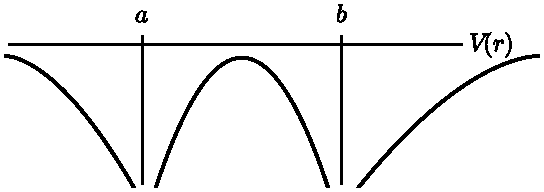
\includegraphics[width=0.8\textwidth]{fig_1.pdf}
\caption*{图 1}
\end{figure}
在本例中，如果我们选取一个以 $a$ 为中心的函数 $\phi_a(\mathbf{r})$，这样的函数便是 $\phi_a+\phi_b$ 与 $\phi_a-\phi_b$，它们分别是偶函数与奇函数。自洽场可以被强制去严格保持 $V(\mathbf{r})$ 原有的对称性，做法有多种。在本例中这很容易：如果我们把每个电子都放入 $(\phi_a+\phi_b)/\sqrt{2}=\phi_{\mathrm{even}}$，一个自旋向上、一个自旋向下，那么显然就保持了一个偶的 $V(\mathbf{r})$。另一种做法（在更复杂的条件下）是把属于某一给定不可约表示（irreducible representation）的所有态都填满，即填满一个“壳层”（shell）或一个“能带”（band）。在这两种情形下我们都保持原有的对称性——在原子中是球对称，在固体中是周期对称。

当质子相距较近时，上述解确实是正确的解，相当接近 $H_2$ 分子的基态；实际上我们已经构造出了这个分子的分子轨道（molecular orbital）波函数。但当质子相距很远时，把一个自旋向上的电子放入 $\phi_a$、把第二个自旋向下的电子放入 $\phi_b$，就可以得到一个好得多的解。这就是 Heitler-London 途径，或至少与它十分接近。在分子轨道解中，当分子相距很远时，两个电子有一半的时间待在\emph{同一个}原子上，因而在分离原子近似下，波函数一半是 $H+H$，一半是 $p+H^-$；而后者的能量远高于前者。系统在 $p+H^-$ 附近存在真实的激发态，在 $H+H$ 附近也存在真实的态，但 M.O.\ 波函数与任何真实激发态都没有多少相似之处。这是 Hartree-Fock 中的一种危险，它时而被人忽视——一个十分良好的自洽解甚至可能不接近任何真实激发态。

在现代多体理论中已经发展出一些检验办法 (17)——我不打算在此讨论——用以验证一个给定的解相对于邻近的其他解是否局域稳定，也就是说，它相对于其他行列式型函数是极小还是极大。这多半能把此处的困难排除掉，但并非在所有情形中都必然如此。

在原子相距很远的情形下，这个例子还说明了第二点。这就是：Hartree-Fock 方程的一个自洽解——它可能像本例中那样是正确的解——往往仍是一个不能令人满意的问题最终本征函数，因为它没有充分地把诸对称性考虑进去。我们在这里构造的行列式波函数是：自旋向上的电子处于波函数 $\phi_a$，自旋向下的电子处于 $\phi_b$：把它记作
\begin{align*}
\Psi_{a\uparrow b\downarrow}&=\frac{1}{\sqrt{2}}
\begin{vmatrix}
\phi_a(1)\,\alpha_1 & \phi_a(2)\,\alpha_2\\
\phi_b(1)\,\beta_1 & \phi_b(2)\,\beta_2
\end{vmatrix}\\
&=\phi_a(1)\phi_b(2)\,\alpha_1\beta_2-\phi_a(2)\phi_b(1)\,\beta_1\alpha_2
\end{align*}
那么 $\Psi_{a\downarrow b\uparrow}$ 呢？就对称性而言，它其实是一个完全等价的波函数；而两者都不是令人满意的总波函数，因为两者都不按对称群的一个不可约表示变换。正确的波函数是
\begin{align*}
\Psi_{\text{singlet}}&=\Psi_{a\uparrow b\downarrow}-\Psi_{a\downarrow b\uparrow}\\
&=\frac{1}{2}\Big[\phi_a(1)\phi_b(2)+\phi_a(2)\phi_b(1)\Big]\big(\alpha_1\beta_2-\alpha_2\beta_1\big)
\end{align*}
以及
\begin{align*}
\Psi_{\text{triplet}}&=\Psi_{a\uparrow b\downarrow}+\Psi_{a\downarrow b\uparrow}\\
&=\frac{1}{2}\Big[\phi_a(1)\phi_b(2)-\phi_a(2)\phi_b(1)\Big]\big(\alpha_1\beta_2+\alpha_2\beta_1\big)
\end{align*}
它经由一个自旋转动与真正的 Hartree-Fock 解
\begin{align*}
\Psi_{a\uparrow b\uparrow}&=\frac{1}{\sqrt{2}}
\begin{vmatrix}
\phi_a(1)\,\alpha_1 & \phi_b(1)\,\alpha_1\\
\phi_a(2)\,\alpha_2 & \phi_b(2)\,\alpha_2
\end{vmatrix}\\
&=\frac{1}{\sqrt{2}}\ \alpha_1\alpha_2\left(\phi_a(1)\phi_b(2)-\phi_a(2)\phi_b(1)\right)
\end{align*}
等价，并且类似地与 $\Psi_{a\downarrow b\downarrow}$ 等价。

尽管如此，如果我们愿意越出这一方法之外，依靠我们关于自旋本征函数的知识，那么从 Hartree-Fock 不仅可以得到三重态（triplet）的能量，也可以得到单态（singlet）的能量。这可以通过比较 $\Psi_{a\uparrow b\downarrow}$ 与 $\Psi_{a\uparrow b\uparrow}$ 的能量来做到。在 Hartree-Fock 中，这两个能量相差某一项，它来自我们在式 (1) 中导出的平行自旋情形下两个电子的附加关联（译注：原书此处作 “Eq. (1)”；但本章编号公式 (1) 在 A.2 节，与此处所指不符，当系讲义原稿残留的引用，所指应即下式中的交换项。）：
\begin{equation*}
\rho(\mathbf{r}_1,\mathbf{r}_2)=\rho_{\text{product}}-\psi_1^*(\mathbf{r}_1)\psi_2^*(\mathbf{r}_2)\psi_2(\mathbf{r}_1)\psi_1(\mathbf{r}_2)
\end{equation*}
由此导致一个能量差
\begin{equation*}
J=\int d\mathbf{r}_1\,d\mathbf{r}_2\ \mathcal{H}(r_{12})\left(\psi_1^*\psi_2(\mathbf{r}_1)\right)\left(\psi_2^*\psi_1(\mathbf{r}_2)\right)
\end{equation*}
现在，Dirac-Van Vleck 矢量模型告诉我们，各个态的能量必须按算符乘积 $J\,\boldsymbol{\sigma}_a\cdot\boldsymbol{\sigma}_b$ 依赖于自旋；在前一情形中它的平均值为 $J/4$，在后一情形中为 $-J/4$。而真正的单态，其能量为 $-3J/4$；于是我们可以通过由 $a\uparrow b\downarrow-a\uparrow b\uparrow$ 之差求出交换积分（exchange integral）来估计单态的能量。

这一技术有两个教益。第一，在诸如自旋问题这类情形中——即我们对相互作用的形式拥有额外的知识、而单靠 Hartree-Fock 又不会立即给出正确对称类型的本征函数的情形——只要稍具巧思，往往就能走得远远超出 Hartree-Fock。同样类型的技巧如今也被用于诸如非球形核的转动等问题：在那里 Hartree-Fock 给出一个椭球形的自洽场，它显然不满足“波函数必须是角动量的本征函数”这一必要要求；但人们可以相当人为地取出 Hartree-Fock 解并使它转动，迫使它具有正当解的形式 (13)。

第二个教益涉及无限系统中的同类问题——例如，设想我们讨论的是一整个由相距很远的原子组成的晶格，如反铁磁体（antiferromagnet）中那样。在这样的大系统中常常出现这样的情形：问题的真正解其实是 Hartree-Fock 的非对称解，而不是某个对称的替代品——例如，反铁磁体的真实基态其实并\emph{非}单态，毋宁说每个原子都\emph{带有}一个确定的自旋。但是，当两个 Hartree-Fock 解在\emph{无限}系统中彼此不同时，由于自洽的特殊性质，新的、非常实在的困难便出现了。这就是说，为了从一个解过渡到另一个解，$N\to\infty$ 个（译注：原文为“N—∞”）Hartree-Fock 本征函数中的每一个都必须经历一次正则变换（canonical transformation），于是这个变换在某种意义上是无穷多个幺正变换（unitary transformation）的乘积。这意味着两个态的交叠基本上为零——场论学家们把这种局面弄得令人生畏，他们说这两个态实际上处在不同的 Hilbert 空间之中。尽管如此，在无限系统中两个自洽解可以定性地完全不同——其差别之大，犹如同一物质的两个相，比如说一个固相与一个液相——这一事实具有重大的意义与重要性。类似的现象也出现在超导之中，甚至出现在固体凝聚这个日常问题里——我们所处理的这块物质可以抛弃其基本哈密顿量的某一个对称元素，建立起它自己的非对称自洽场。这些问题将在本讲义的最后一部分中更充分地加以讨论。

\subsection{自洽方程的推导：二次量子化}

% ---- 原书 p.15 (PDF p030) ----
所有这些，相对于把 Hartree-Fock 理论应用于固体中的电子这一正题来说，已经是相当一段题外话了。为了进一步强调 Hartree-Fock 背后的物理，并顺便毫不费力地多导出几个结果——例如 Koopmans 定理——我将在这里给出从变分原理（variational principle）导出 Hartree-Fock 的基本推导的一个相当不寻常的版本。这同时也可以用来引入产生（creation）与湮灭（destruction）算符的概念，它们在本课程后面的部分将会用到。标准的推导可以在许多教科书中找到（例如可参见文献 2 和 11）。

正如我先前所说，表示一个多粒子波函数

\begin{equation*}
\Psi(r_1\ldots r_N)
\end{equation*}

的实际上唯一可行的办法，是借助乘积函数

\begin{equation*}
\phi_1(r_1)\,\phi_2(r_2)\ldots\ \phi_N(r_N)
\end{equation*}

当然，这是一种非常特殊的多电子函数；但可以证明，任何实际合理的多粒子波函数都可以用足够数目的这类乘积线性展开——例如，多变量 Fourier 积分便正是这样一种展开。

% ---- 原书 p.16 (PDF p031) ----
像这样一个简单的乘积，对于一组全同的量子力学粒子来说并不是合适的波函数，因为这些粒子在原则上不可分辨。正如大家都知道的，自然界中出现的粒子只有两类：或者是 Bose 粒子，对它们要求对称波函数；或者是 Fermi 粒子，它们只具有反对称波函数。在两种情形下都存在该乘积的一个合适的推广：对 Bose 粒子，是对称化乘积（symmetrized product）

\begin{equation*}
(N!)^{-1/2}\sum_P \phi_1(Pr_1)\,\phi_2(Pr_2)\ldots
\end{equation*}

而对 Fermi 粒子，则是反对称化乘积（antisymmetrized product），即行列式（determinant）

\begin{equation*}
(N!)^{-1/2}\sum_P (-1)^P\,\phi_1(Pr_1)\ldots
\end{equation*}

在这些波函数中，唯一有意义的信息只是这样一个事实：一个粒子处在 $\phi_1$ 中，另一个处在 $\phi_2$ 中，等等。事实上，如果我们当初是从一个正交归一集合中选取这些 $\phi$ 的，那么标记这个函数的一个合理方式便是

\begin{equation*}
\Psi(r_1\ldots r_N)\ \longleftrightarrow\ \Psi(n_1 \text{ 在 } \phi_1 \text{ 中，} n_2 \text{ 在 } \phi_2 \text{ 中，} \ldots)\ =\ \Psi(n_1,n_2,n_3\ldots)
\end{equation*}

这称为"n"表示，或"占据数表示"（occupation number representation）。当然，对费米子而言，直接计算表明 $n$ 只能取 0 或 1；而对玻色子，$n$ 可以取任何值。例子：

\begin{equation*}
\Psi(n_1=1,\ n_2=0,\ n_3=0\ldots)\ \text{对应于}\ \phi_1(r_1)
\end{equation*}

\begin{equation*}
\Psi(n_1=1,\ n_2=1,\ n_3=0\ldots)\ \longleftrightarrow\ \frac{1}{\sqrt{2}}\left(\phi_1(1)\phi_2(2)\pm\phi_1(2)\phi_2(1)\right)
\end{equation*}

等等。

这可以简单地看成是从一组变量到另一组变量的一个线性幺正变换（unitary transformation）。看出这必定如此的一个办法，是利用选取 $\phi$ 的自由，采用一组特别简单的函数，即 $\delta$ 函数 $\delta(r-R)$ 那一组，这时 $\phi_n$ 的函数指标 $n$ 便成了连续变量 $R$。函数 $\Psi(n_R=1,\ n_{R'\neq R}=0)$ 是有一个粒子肯定位于 $R$ 处的函数；而任何一个单粒子函数都可以通过幺正变换

\begin{equation*}
\phi(R)\ \longleftrightarrow\ \int dR\ \phi(R)\,\Psi(n_R=1,\ n_{R'\neq R}=0)
\end{equation*}

得到，而这个式子随即给出幺正变换

\begin{equation*}
\Psi(n_\phi=1,\ n_{\phi'\neq\phi}=0)\ =\ \int dR\ \phi(R)\,\Psi(n_R=1,\ n_{R'}=0)
\end{equation*}

其中波函数 $\phi(R)$ 所扮演的角色，正如在普通的单粒子理论中那样，是 $r$ 空间表象与 $\phi$ 表象之间的幺正变换 $(R\,|\,\phi)$。类似的技术也可以用来把任何具有恰当反对称性的 $n$ 粒子函数，用由"一个粒子在 $R_1$ 处、第二个粒子在 $R_2$ 处"等等所标记的函数表示出来。（此后我们把自己限于费米子。）

% ---- 原书 p.17 (PDF p032) ----
因此，占据数表示只不过是把展开式用行列式波函数（determinantal wave functions）写出的一种方便方式。当人们再引入另外几种量子力学算符，即所谓"产生"与"湮灭"算符——它们作用于这些函数的方式，是在某一个特定波函数中添加或移除——即产生或消灭——一个粒子——便开始得到形式上更简单、也更为有用的结果。

如果我们有一组已经正交归一化的函数 $\phi_n$，我们就引入一个算符 $C_{\phi_n}^{\dagger}$，或更简单地记作 $C_n^{\dagger}$，当它作用在任何 $n$ 表示函数 $\Psi(n_1,n_2,\ldots,n_N)$ 上时，便在态 $\phi_n$ 中添加一个新粒子。也就是说，

\begin{equation*}
C_n^{\dagger}\ \Psi(n_1,n_2,\ldots,n_n\ldots)\ =\ \Psi(n_1,n_2,\ldots,n_n+1\ldots)
\end{equation*}

我们还引入它的厄米共轭（hermitian conjugate）$C_n$，它恰好起相反的作用：使 $n_n$ 减一，也就是说，消灭一个处在态 $n$ 中的粒子。有两点值得注意：第一，事实上，对费米子来说，含有两个或更多个处于态 $n$ 的粒子的行列式为零，所以当它作用在 $n_n=1$ 或更大的态 $\Psi$ 上时 $C_n^{\dagger}=0$。这一点用 $(C_n^{\dagger})^2=(C_n)^2=0$ 来表述最为简捷。第二，波函数的相位——因而甚至连它的正负号——迄今为止都还没有被这个定义所确定。于是，如果我们有波函数

\begin{equation*}
\Psi(0\ldots n_1=1,\,0\ldots)\ \longleftrightarrow\ \phi_1(r)
\end{equation*}

那么我们还不知道该给行列式

\begin{equation*}
C_{n_2}^{\dagger}\ \Psi(0\ldots n_1=1,0\ldots)\ =\ \Psi(0\ldots n_1=1,\ n_2=1,0\ldots)
\end{equation*}

以什么相位：是说它是

\begin{equation*}
\frac{1}{\sqrt{2}}\left(\phi_1(r_1)\phi_2(r_2)-\phi_1(r_2)\phi_2(r_1)\right)
\end{equation*}

还是反过来，抑或给相应的行列式一个任意的相位因子。

% ---- 原书 p.18 (PDF p033) ----
事实上，当然，在这种情形下相位是任意的，因为物理结果不可能依赖于它。然而，在比较用不同方式产生粒子而构建起来的两个行列式时，相位就是有关系的了——例如，我们可能想把上面的波函数——它可以写成 $C_2^{\dagger}(C_1^{\dagger}\,|\,\Psi_{\mathrm{vac}})$——与先把粒子产生到态 $\phi_2$ 中、然后再产生到态 $\phi_1$ 中的那个波函数 $C_1^{\dagger}(C_2^{\dagger}\Psi_{\mathrm{vac}})$ 相比较。显然，如果把第一个写成

\begin{equation*}
\frac{1}{\sqrt{2}}\ e^{if}\ \left(\phi_1(r_1)\phi_2(r_2)-\phi_2(r_1)\phi_1(r_2)\right)
\end{equation*}

那么第二个就必须是

\begin{equation*}
\frac{1}{\sqrt{2}}\ e^{if}\ \left(\phi_2(r_1)\phi_1(r_2)-\phi_1\phi_2\right)
\end{equation*}

（译注：原书末项排印为 $\phi_1\phi_2$，漏去了宗量；按上下文应为 $\phi_1(r_1)\phi_2(r_2)$。）它恰恰是第一个的负值。于是，这可以通过规定

\begin{equation*}
C_1^{\dagger} C_2^{\dagger}(\Psi_{\mathrm{vac}})\ =\ -C_2^{\dagger} C_1^{\dagger}\left|\Psi_{\mathrm{vac}}\right)
\end{equation*}

或者

\begin{equation*}
\left(C_1^{\dagger} C_2^{\dagger}+C_2^{\dagger} C_1^{\dagger}\right)\left|\Psi_{\mathrm{vac}}\right)\ =\ 0
\end{equation*}

来描述。事实上，你可以立刻看出：为了确保波函数在 $r_1$ 与 $r_2$ 互换时保持反对称，而我们指明哪一个是 $r_1$、哪一个是 $r_2$ 的唯一途径就是产生算符乘积中因子的次序，因此只需让不同 $n$ 的产生算符彼此\emph{反对易}（anticommute）便已足够：$C_1^{\dagger}C_2^{\dagger}+C_2^{\dagger}C_1^{\dagger}=0$，只要作用在任何波函数上都如此。

这条反对易规则使得把诸 $C^{\dagger}$ 用矩阵显式表示出来变得极其复杂，因此，尽管这样的表示可以找到，我们在这里不打算给出。

通过取厄米共轭你可以看出 $C_n C_{n'}+C_{n'}C_n=0$，而且 $C_n^2=C_n^{\dagger 2}=0$ 其实恰好就是这条规则的 $n=n'$ 那个元素。这一点自己可以做出——我把它留作练习——即 $C_n C_{n'}^{\dagger}+C_{n'}^{\dagger}C_n=0$，当 $n'\neq n$ 时也成立。

% ---- 原书 p.19 (PDF p034) ----
这就只剩下 $C_n^{\dagger}C_n$ 和 $C_nC_n^{\dagger}$ 了。这两个乘积其实非常简单。考虑它们对 $\Psi_0=\Psi(\ldots n_n=0,\ldots)$ 和对 $\Psi_1=\Psi(\ldots n_n=1,\ldots)$ 的作用；省略号代表所有其余指标的一组相同的取值。

\begin{equation*}
C_n^{\dagger} C_n\,\Psi_0\ =\ 0\quad\text{因为}\quad C_n\,\Psi_0=0
\end{equation*}

\begin{equation*}
C_n C_n^{\dagger}\,\Psi_1\ =\ 0\quad\text{因为}\quad C_n^{\dagger}\,\Psi_1=0
\end{equation*}

\begin{equation*}
C_n^{\dagger}\,\Psi_0\ =\ \pm\Psi_1\qquad\quad C_n\,\Psi_1\ =\ \pm\Psi_0
\end{equation*}

相位未定，但它们必须相同，于是

\begin{equation*}
C_n C_n^{\dagger}\,\Psi_0\ =\ \Psi_0\qquad\quad C_n^{\dagger} C_n\,\Psi_1\ =\ \Psi_1
\end{equation*}

既然所有波函数都可以写成这两种类型的线性组合，这些方程就意味着：对所有 $\Psi$，

\begin{equation*}
C_n^{\dagger} C_n+C_n C_n^{\dagger}\ =\ 1;\ \text{因而}\ C_n^{\dagger} C_{n'}+C_{n'}C_n^{\dagger}\ =\ \delta_{nn'}
\end{equation*}

我们还看到，算符 $C_n^{\dagger}C_n$ 就是\emph{测量}处于态 $n$ 中电子数目的那个算符。

\begin{equation*}
C_n^{\dagger} C_n\ =\ n_n\qquad\quad C_n C_n^{\dagger}\ =\ 1-n_n
\end{equation*}

到这里，我们已经证明了：利用占据数表示以及产生与湮灭算符，能够建立起行列式波函数的一套完整的代数——事实上，我们可以把前者弃置不用，而总是从真空出发，写成

\begin{equation*}
\Psi(n_1,n_2,\ldots,n_N,\ldots)\ =\ (C_1^{\dagger})^{n_1}(C_2^{\dagger})^{n_2}\ldots(C_N^{\dagger})^{n_N}\ldots\ \Psi_{\mathrm{vac}}
\end{equation*}

% ---- 原书 p.20 (PDF p035) ----
为了利用这一点，我们还必须把物理可观测量也用产生与湮灭算符展开。这实际上不难。如何做到这一点，考虑一个简单的单电子空间势 $V(r)$ 的情形就能最简单地予以说明。先看 $V(r)$ 作用在一个单电子函数上的效果。如果我们有一组正交函数 $\phi_n(r)$，

\begin{equation*}
V(r)\phi_n(r)\ =\ \sum_m V_{mn}\phi_m(r)
\end{equation*}

（译注：原书右端排印为 $\phi_n(r)$，按上下文应为 $\phi_m(r)$。）$V_{mn}$ 是通常的矩阵元（matrix element）$\int\phi_m^*\,V\phi_n\,dr$。于是，就单电子函数而言，$V(r)$ 的效果与

\begin{equation*}
V\ \longleftrightarrow\ \sum_{m,n} C_m^{\dagger} V_{mn} C_n
\tag{1}
\end{equation*}

相同，这只要把它作用在 $C_n^{\dagger}\Psi_{\mathrm{vac}}\leftrightarrow\phi_n(r)$ 上便可以看到。

类似地，在一个双电子问题中，由不可分辨性我们知道 $V(r)$ 必须作用在两个坐标上，因此我们把 $V(r_1)+V(r_2)$ 插入所研究的哈密顿量或其他可观测量之中。计算它作用在乘积 $\phi_m(r_1)\phi_{m'}(r_2)$ 上的效果，我们得到

\begin{equation*}
\sum_n\left[\phi_n(r_1)\,\phi_{m'}(r_2)\,V_{nm}\ +\ V_{nm'}\,\phi_m(r_1)\,\phi_n(r_2)\right]
\end{equation*}

这又恰好是这样的效果：消灭 $m$ 或 $m'$ 中的任何一个，乘上相应的 $V$，再换上 $n$；也就是说，还是同一个算符。（我留给读者一个练习：证明诸 $C$ 的反对易性再加上反对称化，会导致行列式的正确符号。）

现在只差最后一步，就会使在这套理论中构造可观测量——例如哈密顿量——的一般规则变得一目了然。让我们作正则变换（canonical transformation），变换到 $\delta$ 函数 $\delta(r-R)$，以及相应的产生与湮灭算符 $\Psi^{\dagger}(R)$、$\Psi(R)$。这里采用记号 $\Psi^{\dagger}$ 与 $\Psi$，是因为这些算符常常被称为\emph{电子场}（electron field）算符，它们与普通 Schrödinger 方程中的波函数 $\Psi$ 扮演着十分相似的角色；它们正是这一 c 数量（c-number）的算符版本——故名"二次量子化"。这个变换当然是

% 原书在 $\phi_m$ 上方以箭头标注 $(m|R)$，指明 $\phi_m(R)$ 即幺正变换矩阵元 $(m|R)$
\begin{equation*}
C_m^{\dagger}\ =\ \int dR\ \overset{(m|R)}{\phi_m}(R)\ \Psi^{\dagger}(R)
\tag{2}
\end{equation*}

% ---- 原书 p.21 (PDF p036) ----
然后用 $(R'|m)=\phi_m^{\dagger}$ 遍乘两边并求和，我们便得到逆变换

\begin{equation*}
\sum_m \phi_m^{*}(R')\,C_m^{\dagger}\ =\ \int dR\ \sum_m (R'|m)(m|R)\,\Psi^{\dagger}(R)
\end{equation*}

而且我们认出和式中的 $\delta$ 函数：$\sum_m (R'|m)(m|R)=\delta(R'-R)$，

\begin{equation*}
\Psi^{\dagger}(R')\ =\ \sum_m C_m^{\dagger}\phi_m^{*}(R')
\tag{3}
\end{equation*}

把式 (2) 代入式 (1)，我们得到

\begin{align*}
V\ \longleftrightarrow\ \sum_{m,n}\int dR&\int dR'\ \phi_m(R)\Psi^{\dagger}(R)\int dR''\ \phi_m(R'')\\
&\times\ V(R'')\phi_n(R'')\phi_n^{*}(R')\ \Psi(R')
\end{align*}

再一次，这些和式引入一系列 $\delta$ 函数，于是我们得到

\begin{equation*}
V\ \longleftrightarrow\ \int dR\ \Psi^{\dagger}(R)V(R)\Psi(R)
\end{equation*}

这个公式看上去是不言自明的。积分号下的量常常被称为一个"密度"——在这个情形下是一个"势密度"（potential density）。

我再一次留给读者去证明：这条显然的规则也可以应用于相互作用势

\begin{align*}
\frac{1}{2}\sum_{i,j}\frac{e^2}{R_{ij}}\ \longleftrightarrow\ V_{\mathrm{int}}\
&=\ \frac{1}{2}\sum_{m,n,l,p} C_m^{\dagger} C_n^{\dagger} C_l C_p\, V_{mnlp}\\
&=\ \frac{1}{2}\sum_{\sigma,\sigma'}\int dR\,dR'\ \Psi_{\sigma}^{\dagger}(R)\Psi_{\sigma'}^{\dagger}(R')\ \frac{e^2}{|R-R'|}\ \Psi_{\sigma'}(R')\Psi_{\sigma}(R)
\end{align*}

\begin{equation*}
V_{mnlp}\ =\ e^2\int dR\int dR'\ \frac{\phi_m^{*}(R)\phi_n^{*}(R')\phi_l(R')\phi_p(R)}{|R-R'|}\ \delta_{\sigma_m\sigma_p}\,\delta_{\sigma_n\sigma_l}
\tag{4}
\end{equation*}

% 衔接说明：本文件首句承上文件（p036，式 (4) 之后）关于“密度”的讨论；
% 原书 p042 末尾（本文件最后一式之后）即转入大节 B（ENERGY BANDS IN SOLIDS），不属本文件。

而相应地，我们也可以写出一个动能密度，于是
\begin{equation*}
\mathcal{H} = \sum_{\sigma} \int \mathrm{d}R\;\Psi_{\sigma}^{\dagger}(R)\left(-\frac{\hbar^2\nabla^2}{2m} + V(R)\right)\Psi_{\sigma}(R) + V_{\mathrm{int}}
\tag{5}
\end{equation*}

这种以场算符写出的形式之所以有用，主要在于它可以按我们愿意使用的任意一组单电子函数来展开。

现在，我们终于可以在这一表述框架（formalism）中着手推导 Hartree-Fock 方程和 Koopmans 定理（Koopmans' theorem）了。如果我们利用这样一个自由——在可以借以表示式 (5) 的各组可能的 $\phi_n$ 之间自由变换——把一切都用我们希望最终得到的那组解来表示，那么这两个问题的证明都最为容易。也就是说，我们选取一组 $\phi_n$，使其中的前 $N$ 个是最低能量的行列式波函数中被占据的态。于是，这个最低能量函数便写作
\begin{equation*}
\Psi_N = \prod_{n=1}^{N} C_n^{\dagger}\,\Psi_{\mathrm{vac}}
\end{equation*}

若要 $\Psi_N$ 具有最低能量，我们就必须要求
\begin{equation*}
E_N = \frac{\left(\Psi_N,\, \mathcal{H}\Psi_N\right)}{\left(\Psi_N,\, \Psi_N\right)}
\end{equation*}
取极小，因而也就是要求
\begin{equation*}
\left(\delta\Psi_N,\, \mathcal{H}\Psi_N\right) = 0
\end{equation*}
这里我们略去了第二个 $\Psi$ 的变分，因为它给出的恰恰是复共轭，而归一化我们稍后再作保证。

依次变动组成 $\Psi_N$ 的每一个 $\phi_n$——也就是变动每一个 $C_n^{\dagger}$——便可以顾及 $\Psi_N$ 的一切可能的无穷小变分。这样我们就必须保证
\begin{equation*}
\left(\delta C_n^{\dagger}\left(\prod_{m\neq n}^{N} C_m^{\dagger}\right)\Psi_{\mathrm{vac}}\,,\; \mathcal{H}\, C_n^{\dagger} \prod_{m\neq n}^{N} C_m^{\dagger}\,\Psi_{\mathrm{vac}}\right) = 0
\end{equation*}

若把 $\delta C_n^{\dagger}$ 取作诸 $C_m^{\dagger}$ 的任意线性组合：$\delta C_n^{\dagger} = \sum_m \delta_m C_m^{\dagger}$，那么，为保证归一化，我们可以假定 $\delta_{m=n}$ 为零；而其余那些 $m < N$ 的项都自动给出零，因为 $(C_m^{\dagger})^2 = 0$。于是我们的检验函数是 $\delta C_n^{\dagger} = \sum_{m>N} \delta_m C_m^{\dagger}$；实际上我们可以要求：对一切 $M > N$，$n \leq N$：
\begin{equation*}
\left(C_M^{\dagger} \prod_{m\neq n}^{N} C_m^{\dagger}\,\Psi_{\mathrm{vac}}\,,\; \mathcal{H} \prod_{m}^{N} C_m^{\dagger}\,\Psi_{\mathrm{vac}}\right) = 0
\tag{6}
\end{equation*}

直接计算这个式子确实会给出 Hartree-Fock 方程；但我愿意走一条更物理的路线，并同时演示 Koopmans 定理。

把式 (5) 中的 $\mathcal{H}$ 按我们假定的一组解展开，便得到
\begin{equation*}
\mathcal{H} = \sum_{m,n} \mathcal{H}^1_{mn}\, C_m^{\dagger} C_n + \frac{1}{2}\sum_{lmnp} V_{lmnp}\, C_l^{\dagger} C_m^{\dagger} C_n C_p
\end{equation*}
其中 $\mathcal{H}^1$ 是 (5) 中的单电子部分：
\begin{equation*}
\mathcal{H}^1_{mn} = \int \phi_m^{*}(r)\left(\frac{p^2}{2m} + V\right)\phi_n(r)\,\mathrm{d}r
\end{equation*}
$V_{lmnp}$ 已在前面由式 (4) 定义。

现在让我们来计算 $\mathcal{H}$ 与被占据态之一的产生算符 $C_n^{\dagger}$ 的\emph{对易子}（commutator）。直截了当地运用我们的反对易关系，即可看到
\begin{align*}
\left[C_l^{\dagger} C_p,\, C_n^{\dagger}\right] &= C_l^{\dagger} C_p C_n^{\dagger} - C_n^{\dagger} C_l^{\dagger} C_p = -\,C_l^{\dagger} C_n^{\dagger} C_p - C_n^{\dagger} C_l^{\dagger} C_p = 0\\
\left[C_n^{\dagger} C_p,\, C_n^{\dagger}\right] &= 0\\
\left[C_l^{\dagger} C_n,\, C_n^{\dagger}\right] &= C_l^{\dagger} C_n C_n^{\dagger} + C_l^{\dagger} C_n^{\dagger} C_n = C_l^{\dagger}\\
\left[C_n^{\dagger} C_n,\, C_n^{\dagger}\right] &= C_n^{\dagger}
\end{align*}

规则便是：若两个算符的乘积中不含 $C_n$，它就与 $C_n^{\dagger}$ 对易；否则我们就把 $C_n$ 湮灭掉，而留下一个落单的 $C_n^{\dagger}$ 算符。因此，与一个产生算符的对易子所产生的效果，与该算符本身的作用大体相同。注意
\begin{equation*}
\left[C_a^{\dagger} C_b,\, C_c^{\dagger}\right]^{\dagger} = -\left[C_b^{\dagger} C_a,\, C_c\right]
\end{equation*}
因此，穿过一个湮灭算符作对易，得到的将是带一个负号的共轭结果。

$C_n^{\dagger}$ 穿过四算符乘积的对易子，其符号取决于 $C_n$ 出现在两个可能位置中的第一个还是第二个：
\begin{align*}
\left[C_a^{\dagger} C_b^{\dagger} C_l C_m,\, C_n^{\dagger}\right] &= 0\qquad l,\, m \neq n\\
\left[C_a^{\dagger} C_b^{\dagger} C_l C_n,\, C_n^{\dagger}\right] &= C_a^{\dagger} C_b^{\dagger} C_l\\
\left[C_a^{\dagger} C_b^{\dagger} C_n C_l,\, C_n^{\dagger}\right] &= -\,C_a^{\dagger} C_b^{\dagger} C_l
\end{align*}
最后一式是因为：$C_n$ 必须先穿过 $C_l$ 作反对易，然后才能去湮灭 $C_n^{\dagger}$。

利用这些简单的规则，我们得到
\begin{equation*}
\left[\mathcal{H},\, C_n^{\dagger}\right] = \sum_m \mathcal{H}^1_{mn}\, C_m^{\dagger} + \frac{1}{2}\sum_{mlp}\left(V_{mlpn} - V_{mlnp}\right) C_m^{\dagger} C_l^{\dagger} C_p
\tag{7}
\end{equation*}

最后，让我们把这个结果用于计算能量变分，即式 (6)。我们让任一个 $C_n^{\dagger}$ 穿过哈密顿量 $\mathcal{H}$ 作对易；这就给出
\begin{align*}
0 = {}& \left(C_M^{\dagger} \prod_{m\neq n}^{N} C_m^{\dagger}\,\Psi_{\mathrm{vac}}\,,\; C_n^{\dagger}\,\mathcal{H} \prod_{m\neq n}^{N} C_m^{\dagger}\,\Psi_{\mathrm{vac}}\right)\\
&+ \left(C_M^{\dagger} \prod_{m\neq n}^{N} C_m^{\dagger}\,\Psi_{\mathrm{vac}}\,,\; \left[\mathcal{H},\, C_n^{\dagger}\right] \prod_{m\neq n}^{N} C_m^{\dagger}\,\Psi_{\mathrm{vac}}\right)
\tag{8}
\end{align*}

第一项立即为零，因为态 $n$ 在右边的态中肯定被占据，而在左边的态中肯定未被占据。于是剩下的就是含对易子的那个标量积项：即上文式 (8) 中的第二项。

如果 $\left[\mathcal{H},\, C_n^{\dagger}\right]$ 中没有那些三费米子项，这件事本来很容易解决，只须要求
\begin{equation*}
\mathcal{H}^1_{Mn} = 0\qquad M > N,\; n \leq N
\end{equation*}
也就是说，要求
\begin{equation*}
\left[\mathcal{H},\, C_n^{\dagger}\right] = \sum_{\substack{m\ \text{occupied}\\ \text{only}}} \lambda_{mn}\, C_m^{\dagger}
\end{equation*}
事实上，不同被占据态之间的混合无关紧要；我们总可以通过把诸 $C_n^{\dagger}$ 作线性组合，使矩阵 $\lambda_{mn}$ 对角化，从而找到一组态，使得
\begin{equation*}
\left[\mathcal{H},\, C_n^{\dagger}\right] = E_n\, C_n^{\dagger}
\end{equation*}

在确定三费米子项的效果时，原则上遵循的正是同样的做法。形如 $C_m^{\dagger} C_l^{\dagger} C_p$ 的项在许多情形下会自动给出零；例如，$p$ 必须是某个被占据的态，否则 $C_p\,\Psi_{\mathrm{vac}} = 0$。但如果 $C_p$ 湮灭的是 $j$ 态上的粒子，即 $C_p = C_j$，那么必须有 $C_m^{\dagger}$ 或 $C_l^{\dagger}$ 把它补上，否则标量积将为零；因为左边的态中 $j$ 是被占据的。最后，$M$ 之所以能被占据，唯一的途径是 $C_m^{\dagger}$ 或 $C_l^{\dagger}$ 中的另一个去填它。于是我们有如下两类项：
\begin{equation*}
\left(V_{Mjjn} - V_{Mjnj}\right) C_M^{\dagger}\, n_j \qquad\text{与}\qquad -\left(V_{jMjn} - V_{jMnj}\right) C_M^{\dagger}\, n_j
\end{equation*}

考察 $V$ 的定义即可以看出，它对于内指标与外指标的交换是对称的，因此这两类项完全相同，从而消去了式 (7) 中的 1/2。此外我们还看到 $V_{Mnnn} = V_{Mnnn}$（译注：原文两处下标完全相同，显系排印之误；按正文所述对称性，疑第二处应为 $V_{nMnn}$），因此我们愿意的话，可以对称地插入 $C_n^{\dagger} n_n$ 这一项。因子 $n_j$（占据数算符）作用在乘积函数上时恰好就是 1，于是最终的方程是

\begin{equation*}
0 = \left(C_M^{\dagger} C_n\,\Psi_{\text{H-F}}\,,\; \left[\mathcal{H},\, C_n^{\dagger}\right] C_n\,\Psi_{\text{H-F}}\right) = \mathcal{H}^1_{Mn} + \sum_{m\ \text{occ.}}\left(V_{Mmmn} - V_{Mmnm}\right)
\end{equation*}
或者，
\begin{equation*}
\sum_{\text{all }m}\left(\mathcal{H}^1_{mn}\, C_m^{\dagger} + \sum_{j=1}^{N}\left(V_{mjjn} - V_{mjnj}\right)C_m^{\dagger}\right) = E_n\, C_n^{\dagger}
\tag{9}
\end{equation*}
（同样，我们可以在诸被占据波函数之间重新对角化。）

这个方程确实就是 Hartree-Fock 方程，这一点可以通过变换到空间（电子场）表象来验证。此时式 (9) 即为
\begin{align*}
&\sum_m \int \phi_m^{\dagger}(r)\,\mathcal{H}^1(r)\,\phi_n(r)\,\mathrm{d}r \int \mathrm{d}R\;\phi_m(R)\Psi^{\dagger}(R) \\
&\quad+\sum_j\sum_m \int \mathrm{d}r \int \mathrm{d}r'\;\frac{e^2}{|r-r'|}\left[\phi_m^{*}(r)\phi_j^{*}(r')\phi_j(r')\phi_n(r)\right.\\
&\qquad\left.-\;\phi_m^{*}(r)\phi_j(r')\phi_n(r')\phi_j(r)\right]\int \mathrm{d}R\;\phi_m(R)\Psi^{\dagger}(R)\\
&\quad=E_n \int \mathrm{d}R\;\phi_n(R)\Psi^{\dagger}(R)
\end{align*}
对 $m$ 的求和给出一系列 $\delta$ 函数，使上式化为
\begin{align*}
\int \mathrm{d}R\;\Psi^{\dagger}(R)\;\mathcal{H}^1(R)\,\phi_n(R) &+ \int \mathrm{d}r_2\;\frac{e^2}{|r_2-R|}\;|\phi_j(r_2)|^2\,\phi_n(R) \\
&- \int \mathrm{d}r_2\;\frac{e^2}{|r_2-R|}\;\phi_j^{*}(r_2)\,\phi_n(r_2)\,\phi_j(R) \\
&= \int \mathrm{d}R\;\Psi^{\dagger}(R)\,E_n\,\phi_n(R)
\end{align*}
既然所有 $\Psi^{\dagger}(R)$ 都线性无关，作为 $R$ 的函数，这一系数必须为零；而这个系数正是 Hartree-Fock 方程。证讫（Q.E.D.）。

Koopmans 定理的证明要容易得多。定理说的是：系数 $E_n$ 恰好就是在 Hartree-Fock 近似下把处于 $\phi_n$ 态的电子移走所需的激发能。

作为整体的 Hartree-Fock 态的能量 $E_{\text{H-F}}$ 可以简单地定义为
\begin{equation*}
\mathcal{H}\,\Psi_{\text{H-F}} = E_{\text{H-F}}\,\Psi_{\text{H-F}}\quad(\text{当然，还有非对角项})
\end{equation*}

移走电子 $n$ 之后那个态的总能量则简单地由下式给出：
\begin{equation*}
\mathcal{H} \prod_{m\neq n} C_m^{\dagger}\,\Psi_{\mathrm{vac}} = \epsilon_n \prod_{m\neq n} C_m^{\dagger}\,\Psi_{\mathrm{vac}}
\end{equation*}

利用对易子，我们可以得到一个比较：
\begin{align*}
&C_n^{\dagger}\,\mathcal{H}\left(C_n\,\Psi_{\text{H-F}}\right) - \mathcal{H}\,C_n^{\dagger}\left(C_n\,\Psi_{\text{H-F}}\right)\\
&\quad= \left(\epsilon_n - E_{\text{H-F}}\right)\Psi_{\text{H-F}} = -\left[\mathcal{H},\, C_n^{\dagger}\right] C_n\,\Psi_{\text{H-F}}
\end{align*}

但这最后一个乘积恰恰就是我们在计算 $\delta E$ 时所算过的东西；我们算出的是对角项，并把它\emph{定义}为 $E_n C_n^{\dagger}$；于是
\begin{equation*}
\epsilon_n - E_{\text{H-F}} = E_n
\end{equation*}

把态 $n$ 中的一个电子移走需要花费能量 $E_n$。这就是 Koopmans 定理。

诚然，在这个形式下它并不十分严格，因为 $E_{\text{H-F}}$ 与 $\epsilon_n$ 并不严格可比——它们是电子数不同的两个系统的能量。但可以证明，在讨论由于掏空两个不同的态 $\phi_n$ 而引起的能量差时，$E_n$ 仍然是有意义的量。

这样，参数 $E_n$ 的物理意义就清楚了。它们与总能量 $E_{\text{H-F}}$ 没有直接的关系，因为，当然，$E_n$ 中包含了粒子 $n$ 与所有其他粒子 $m$ 的相互作用能，而当我们移走这个粒子时，这份相互作用能便整个丢失了。如果我们接着移走粒子 $m$，其移出能将不再包含它与 $n$ 的相互作用，尽管 $E_m$ 中确实含有这份能量。因此，在所有 $E_n$ 之和中，必须扣去总相互作用能，以免把相互作用重复计算。于是
\begin{align*}
E_{\text{H-F}} &= \sum_n E_n - \frac{1}{2}\sum_{n,m}\left(V_{nmmn} - V_{nmnm}\right)\qquad\text{或}\\
&= \sum_n \mathcal{H}^1_{nn} + \frac{1}{2}\sum_{n,m}\left(V_{nmmn} - V_{nmnm}\right)
\end{align*}

% （以下两段是上一小节 A.2 在原书页 28 顶部的收尾内容，装配时移走。）

方程 $[\mathcal{H},\,C_n^{\dagger}] = E_n C_n^{\dagger}$（除那些会激发出三个粒子的项之外）本来可以或多或少地先验猜出，以作为 Hartree-Fock 近似之物理内涵的表述。换言之，人们想要做的，是找出一组产生单电子激发的算符，并用这些单电子态中最低的 $N$ 个态来填充。于是，对基态的自洽（self-consistency）性要求就相当于要求：相互作用项在平均意义上、并在我们近似的限度之内，其作用如同施加于我们所选诸态的一个平均势，而不去激发其他单电子态——我们把 $[\mathcal{H},C_n^{\dagger}]$ 视为 $i(\partial C_n^{\dagger}/\partial t)$，并要求时间演化不激发其他的态。全部操作上的复杂之处，并不在于计算 $[\mathcal{H},C_n^{\dagger}]$，而在于证明这样做确使总能量取极小。

上面所述，是把对易子（commutator）与哈密顿量联用——亦即运动方程（equations of motion）——来在多体问题 (18) 中同时确定基态与激发能量的最直截了当的例子之一。这一技术在多体理论的大多数分支中都很有用，尽管它大概正逐渐被一个更普遍、更完备然而与之类似的方法——Green 函数方法——所取代。

\section{固体中的能带}

现在我们接着讨论用 Hartree-Fock 方法计算固体中能带（energy band）时所涉及的问题——它们实际得多，也远不那么形式化。

在这一领域，Reitz (11)、Ham (19) 以及 Wigner 与 Seitz (20) 刊于《Seitzschrift》第 1 卷的文章极有价值，Brooks (21) 的文章与 Jones 的书 (22) 亦然。在讨论能带与内聚能（cohesive energy）的计算时，我将涵盖以下专题：

\begin{enumerate}
\item 弱周期势的微扰论（perturbation theory）——这将使我们获得关于布里渊区（Brillouin zone）与 Jones 区的一些概念。（我不打算谈紧束缚（tight binding）；就能带理论而言，在实际固体中它似乎从来都不是一种很有用的技术。）
\item 元胞法（cellular method）。
\item 自由电子气及其交换能——关于关联能（correlation energy）的简短评述。
\item O.P.W.（正交化平面波，orthogonalized plane wave）与消去理论（cancellation theory）。
\end{enumerate}

\subsection{弱周期势的微扰论：布里渊区与 Jones 区、对称化平面波}

当然，除了极简单的情形，没有人知道如何精确求解——哪怕动用机器——普遍的积分微分 Hartree-Fock 方程。实际使用的种种近似，全都只是基于对某种周期性局域势的估计——电子就在这种势中运动——然后在这个周期势 $V(\mathbf{r})$ 中求解波动方程。正如我们下面将要讨论的，所有这类波动方程的解都具有若干共同的一般性质；这些性质大概最容易在下面这种方案中加以描述——它是所有近似方案中最简单的一种，而且人们现已认识到它粗略地适用于许多金属。

当然，一切能带结构中最简单的，莫过于周期势完全消失的极限下所得的那种。但要理解怎样才能把它看作一种能带结构，我们必须先考察周期势 $V(\mathbf{r})$ 相对较弱的情形。

每一种晶体结构都有一个基本的空间平移群，或称“布拉维格子”（Bravais lattice），它由沿三个线性独立矢量 $\mathbf{a}_1$、$\mathbf{a}_2$、$\mathbf{a}_3$ 的平移构成；这一对称性保证了
\begin{equation*}
V(\mathbf{r} + l\mathbf{a}_1 + m\mathbf{a}_2 + n\mathbf{a}_3) = V(\mathbf{r})
\end{equation*}

选取 $\mathbf{a}_1$、$\mathbf{a}_2$ 与 $\mathbf{a}_3$ 总有无穷多种可能的方式，但它们全都生成同一个晶格，并且具有相同的初基原胞（primitive cell）尺寸
\begin{equation*}
\Omega = \mathbf{a}_1 \cdot (\mathbf{a}_2 \times \mathbf{a}_3)
\end{equation*}

作为这种周期性的一个后果，$V(\mathbf{r})$ 的 Fourier 变换 $V(\mathbf{k})$ 化为一个 Fourier 和而非 Fourier 积分：
\begin{align*}
V(\mathbf{k}) &= \frac{1}{\text{vol.}} \int d\mathbf{r}\; e^{-i\mathbf{k}\cdot\mathbf{r}}\,V(\mathbf{r}) \\
&= \frac{n(\text{cells})}{\text{vol.}} \left( \int_{\text{cell}} d\mathbf{r}\; e^{-i\mathbf{k}\cdot\mathbf{r}}\,V(\mathbf{r}) \right) \sum_{m,l,n} e^{-i\mathbf{k}\cdot(m\mathbf{a}_1 + n\mathbf{a}_2 + l\mathbf{a}_3)}
\end{align*}

除非满足下述条件，否则对 $l$、$m$、$n$ 求和时最后这个和式为零：
\begin{equation*}
\mathbf{k}\cdot\mathbf{a}_1 = 2\pi n_1 \qquad \mathbf{k}\cdot\mathbf{a}_2 = 2\pi n_2 \qquad \mathbf{k}\cdot\mathbf{a}_3 = 2\pi n_3
\end{equation*}
其中 $n_1$、$n_2$ 与 $n_3$ 全为整数。这些关系式只有当 $\mathbf{k}$ 是我们晶体的布拉维格子的倒格子（reciprocal lattice）中的一个矢量 $\mathbf{K} = n_1\mathbf{b}_1 + n_2\mathbf{b}_2 + n_3\mathbf{b}_3$ 时才能被满足。倒格子的基矢 $\mathbf{b}_j$ 可以由 $\mathbf{a}_i\cdot\mathbf{b}_j = 2\pi\delta_{ij}$（译注：原书印作 $2\delta_{ij}$，系漏排 $\pi$）来定义——这就是说，$\mathbf{b}_i$ 垂直于两个晶格矢量，其长度由第三个矢量决定；或者由下式定义：
\begin{equation*}
V(\mathbf{r}) = \sum_k e^{i\mathbf{K}\cdot\mathbf{r}}\,V(\mathbf{K}) \tag{10}
\end{equation*}
（$\mathbf{K}$ 为倒格矢的集合。）

此式可以反过来给出
\begin{equation*}
V(\mathbf{K}) = \frac{1}{N\Omega} \int d\mathbf{r}\; e^{i\mathbf{K}\cdot\mathbf{r}}\,V(\mathbf{r})
\end{equation*}
但由于 $e^{i\mathbf{K}\cdot(\mathbf{r} + l\mathbf{a}_1 + m\mathbf{a}_2 + n\mathbf{a}_3)} = e^{i\mathbf{K}\cdot\mathbf{r}}$，便有
\begin{equation*}
V(\mathbf{K}) = \frac{1}{\Omega} \int_{\text{primitive cell}} d\mathbf{r}\; e^{i\mathbf{K}\cdot\mathbf{r}}\,V(\mathbf{r})
\end{equation*}

晶格对称性的一切后果都总结在式 (10) 的形式之中。

现在我们把 $V(\mathbf{r})$ 代入 Schrödinger 方程。
\begin{equation*}
-\frac{\hbar^2}{2m}\,\nabla^2\Psi(\mathbf{r}) + V(\mathbf{r})\Psi(\mathbf{r}) = E\Psi(\mathbf{r})
\end{equation*}

在没有 $V(\mathbf{r})$ 时，解将为平面波（plane wave）：
\begin{equation*}
\phi_k(\mathbf{r}) = \frac{1}{(N\Omega)^{1/2}}\,e^{i\mathbf{k}\cdot\mathbf{r}} \qquad\qquad -\frac{\hbar^2}{2m}\,\nabla^2\phi_k = -\frac{\hbar^2 k^2}{2m}\,\phi_k = E_k^{0}\,\phi_k
\end{equation*}

在晶体表面上所能施加的最简单边界条件，是 Born-von Karman 周期性边界条件——即设想晶格在 $x$、$y$、$z$ 三个可能方向的每一个方向上都折叠到自身之上，于是三个方向上的长度分别为 $L_1$、$L_2$、$L_3$，且 $L_1L_2L_3 = N$。于是 $\Psi(x+L_1,\,y,\,z) = \Psi(x,y,z)$，从而 $k_xL_1 = 2\pi n_x$，$k_x = 2\pi n_x/L_1$。这样，$\mathbf{k}$ 空间中每一体积 $(2\pi)^3/N\Omega$ 对应一个可能的态，因为每一体积为 $(2\pi)^3/L_1L_2L_3$ 的平行六面体对应一个态（当然，计入自旋则为两个态）。

现在，当我们引入 $V(\mathbf{r})$ 之后，各个平面波态便不再相互独立。然而我们仍然可以希望：若 $V$ 很弱，真实的波函数便主要由单个平面波 $\phi_k$ 构成，于是我们用一个特定的 $\mathbf{k}$ 来标记它们：
\begin{equation*}
\Psi_k = \phi_k + \sum_{k'\neq k} a_{k'}\,\phi_{k'}
\end{equation*}

Schrödinger 方程于是变成下面这组关于 $a_k$ 与 $E_k$ 的耦合线性方程：
\begin{equation*}
E - E_k^{0} = \sum_{k'\neq k} (k'|V|k)\,a_{k'} + (k|V|k)
\end{equation*}
\begin{equation*}
(E - E_{k'}^{0})\,a_{k'} = \sum_{k''\neq k} (k''|V|k')\,a_{k''} + (k|V|k')
\end{equation*}

从 $V$ 的表达式我们立即看出：一般而言，除非 $k' - k$ 等于某个倒格矢 $\mathbf{K}$，否则这些矩阵元（matrix element）为零。矢量 $\mathbf{K} = 0$ 给出一个平均势 $(k|V|k) = V_0$，它只是加到所有能量上的一个平凡常数；其余所有的 $V$ 则起到把 $\mathbf{k}$ 与通过倒格子平移与之相连的某个矢量 $\mathbf{k}+\mathbf{K}$ 耦合起来的作用。因此，我们的波函数实际上必定是
\begin{equation*}
\Psi_k = \phi_k + \sum_{\substack{K\neq 0 \\ \text{(倒格子)}}} a_{k+K}\,\phi_{k+K} \tag{11}
\end{equation*}
而我们的方程组是
\begin{equation*}
(E - E_k^{0})(1) = \sum_K V_K\,a_{k+K} \qquad (\text{即 } a_k = 1)
\end{equation*}
\begin{equation*}
(E - E_{k+K}^{0})\,a_{k+K} = V_K^{*}(1) + \sum_{K'\neq -K} V_{K'}\,a_{k+K+K'}
\end{equation*}

在一般位置处，可以预期微扰论收敛；若果真如此，则我们看到 $a_{k+K}$ 具有 $V_K$ 的量级，于是右端最后一项具有 $V^2$ 的量级，应当略去。这样做的结果是
\begin{equation*}
a_{k+K} \simeq \frac{V_K^{*}}{E - E_{k+K}^{0}}
\end{equation*}
\begin{equation*}
E - E_k^{0} = \sum_K \frac{|V_k|^{2}}{E - E_{k+K}^{0}}
\end{equation*}
（译注：原书此式及下文式 (12) 的分子均印作 $|V_k|^2$，按求和指标应为 $|V_K|^2$。）

最后，若 $V$ 足够小，则 $E \simeq E_k^{0}$，于是得到
\begin{equation*}
E_k = E_k^{0} - \sum_K \frac{|V_K|^{2}}{E_{k+K}^{0} - E_k^{0}} \tag{12}
\end{equation*}

这样，平面波的能谱与平面波函数只不过是受到了微弱的微扰：混入了波矢为 $\mathbf{k}+\mathbf{K}$ 的态，这里 $\mathbf{K}$ 属于倒格子。

值得指出的是，形如式 (11) 的波函数可以写成
\begin{equation*}
\Psi_k = e^{i\mathbf{k}\cdot\mathbf{r}}\left(1 + \sum_{K\neq 0} a_{k+K}\,e^{i\mathbf{K}\cdot\mathbf{r}}\right) = e^{i\mathbf{k}\cdot\mathbf{r}}\,u_k(\mathbf{r})
\end{equation*}
其中，正如我们在展开 $V(\mathbf{r})$ 时所见到的那样，$u_k(\mathbf{r})$ 以晶格周期为周期，因为它是关于倒格子波矢的一个 Fourier 和。这就是 Bloch 的著名结果；它显然不依赖于微扰论的收敛性，而是普遍成立的。

一个相关的事实是：从晶格平移对称性的观点来看，$\phi_k$ 与 $\phi_{k+K}$ 本质上是相同的，因为如果我们施行一个位移为 $\mathbf{A} = l_1\mathbf{a}_1 + l_2\mathbf{a}_2 + l_3\mathbf{a}_3$ 的晶格平移 $T$，则
\begin{equation*}
T\phi_k = e^{i\mathbf{k}\cdot\mathbf{A}}\phi_k \qquad\qquad T\phi_{k+K} = e^{i\mathbf{k}\cdot\mathbf{A}}\phi_{k+K}
\end{equation*}
因此，从群论的角度看，它们具有相同的对称性质，可以预期它们会相互混合；当我们讨论布里渊区时，将会看到这一点的种种后果。

当右端的求和不小时，式 (12) 并不能令人满意；而在 $\mathbf{k}$ 空间中大量位置上情形必然如此，因为存在若干区域，在其中
\begin{equation*}
E_{k+K}^{0} = \hbar^2(\mathbf{k}+\mathbf{K})^2/2\mathrm{m} \simeq \hbar^2 k^2/2\mathrm{m} = E_k^{0}
\end{equation*}
（译注：原书此式第一个系数印作 $h^2$，应为 $\hbar^2$。）

这发生在满足下式的点附近：
\begin{equation*}
2\,\mathbf{k}\cdot\mathbf{K} + K^2 = 0
\end{equation*}

只要 $\mathbf{k}$ 平行于 $\mathbf{K}$ 的分量取值 $-K/2$，而其余两个分量任意，上式就会成立。而且，由于 $-\mathbf{K}$ 也是倒格矢，因此只要 $\mathbf{k}$ 落在平分某一倒格矢的平面上，这种情况就会出现（图 2）。

\begin{figure}[H]
\centering
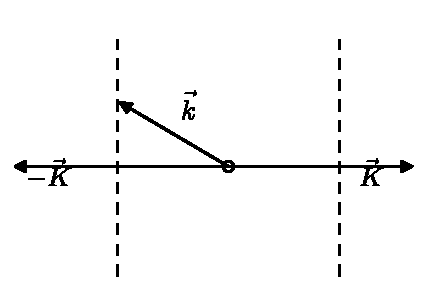
\includegraphics[width=0.72\textwidth]{fig_2.pdf}
\caption*{图 2（原书图注仅 “Figure 2”：波矢 k 与倒格矢 ±K，竖直虚线为平分面）}
\end{figure}

现在，若 $V$ 确实很小，并且 $\mathbf{k}$ 不位于两个这类平面的交线上，那么除了涉及 $\mathbf{K}$ 的那一项之外，微扰求和中的所有其余项我们仍可以用 $E_k = E_k^{0}$ 来近似。这些附加的项于是加起来只给出一个无关紧要的常数修正，而留给我们的只不过是求解波函数中两个强耦合分量的一个二次方程：
\begin{equation*}
E - E_k^{0} = \frac{|V_K|^{2}}{E - E_{k+K}^{0}} + \sum_{K'\neq 0,\,K} \frac{|V_{K'}|^{2}}{E_k^{0} - E_{k+K'}^{0}}
\end{equation*}
或
\begin{equation*}
\left(E - \frac{\hbar^2 k^2}{2\mathrm{m}}\right)\left(E - \frac{\hbar^2 (k+K)^2}{2\mathrm{m}}\right) \simeq |V_K|^{2}
\end{equation*}
（倘若不得已，我们本可以把 $E_k^{0}$ 与 $E_{k+K}^{0}$ \emph{两者}都对其他所有态引起的微扰加以修正。只修正两个能量中的一个是不妥的，因为那会使区边界发生一个非物理的移动。）

令 $\mathbf{k} = \mathbf{K}/2 + k_{\parallel} + k_{\perp}$，其中 $k_{\perp}$ 是沿垂直平分面方向、垂直于 $\mathbf{K}$ 的无关分量，而 $k_{\parallel}$ 是平行于 $\mathbf{K}$ 的分量，即 $\mathbf{k}$ 到该平面的距离。于是上面的方程变为
\begin{align*}
&\left[E - \frac{\hbar^2}{2\mathrm{m}}\left\{\left(\frac{K}{2}\right)^{2} + k_{\parallel}^{2} + k_{\perp}^{2}\right\} + \left(\frac{\hbar^2}{2\mathrm{m}}\right)k_{\parallel}K\right] \\
&\quad\times\left[E - \frac{\hbar^2}{2\mathrm{m}}\left\{\left(\frac{K}{2}\right)^{2} + k_{\perp}^{2} + k_{\parallel}^{2}\right\} - \frac{\hbar^2}{2\mathrm{m}}\,k_{\parallel}K\right] \\
&= |V_K|^{2}
\end{align*}
于是
\begin{align*}
E = {}& \frac{\hbar^2}{2\mathrm{m}}\left[\left(\frac{K}{2}\right)^{2} + k_{\perp}^{2} + k_{\parallel}^{2}\right] \\
&\pm \sqrt{|V_K|^{2} + \left(\frac{\hbar^2}{2\mathrm{m}}\,k_{\parallel}K\right)^{2}}
\end{align*}

图 3 是沿一条 $k_{\perp}$（译注：原文印作 $K_{\perp}$）为常数的线对该方程所作的草图。这表明在布里渊区边界处存在带隙（band gap）$\Delta_K = 2V_K$。因此，周期势所起的作用，是使 $E$–$\mathbf{k}$ 曲线 $E = \hbar^2 k^2/2\mathrm{m}$ 在每一个平面 $(\mathbf{k}\cdot\mathbf{K}) = |\mathbf{K}|^2/2$ 处失去连续性；于是整条曲线的草图看上去可能就像图 4 所示那样。

\begin{figure}[H]
\centering
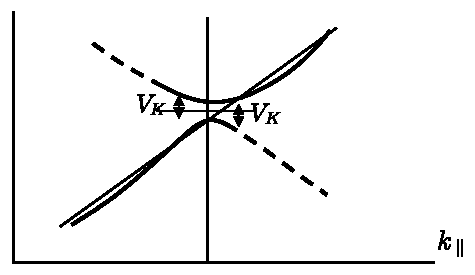
\includegraphics[width=0.72\textwidth]{fig_3.pdf}
\caption*{图 3（原书图注仅 “Figure 3”：沿 $k_\parallel$ 方向的恒能线，自由电子交叉直线在区边界处劈裂，能隙为 $V_K$）}
\end{figure}

\begin{figure}[H]
\centering
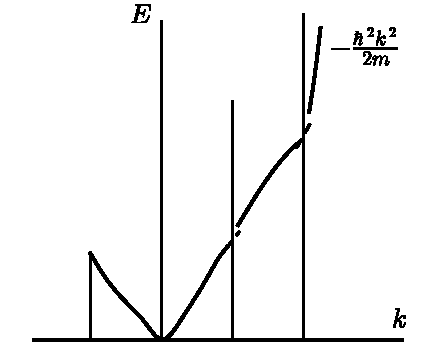
\includegraphics[width=0.72\textwidth]{fig_4.pdf}
\caption*{图 4（原书图注仅 “Figure 4”：$E$–$k$ 曲线整体草图，自由电子抛物线在各区边界处张开隙；图中标注 −ℏ²k²/2m）}
\end{figure}

我们注意到，在这些区边界点的每一处，方程都有一个越过边界继续延伸的形式解。$\mathbf{k}$ 处的这个形式解事实上与 $\mathbf{k}' = \mathbf{k} - \mathbf{K}$ 处的解全同；这一事实例示了一个可以由我们出发的方程容易证明的一般性质：能量可以看作 $\mathbf{k}$ 的连续然而多值的函数，并具有倒格子的周期性：$E(\mathbf{k}+\mathbf{K}) = E(\mathbf{k})$。

从这个观点来看，隙看起来在其中张开的那些平面是相当任意的；它们是由微扰计算挑出来的，而在原则上，在一个足够缺乏对称性的晶格中，这种计算并不给出任何唯一的方案——例如，对于带隙在何处最小、或者能带在何处可能是平坦的，它都给不出唯一答案。尽管如此，对称性通常使得能带结构在 $\mathbf{k}$ 空间中是偶的。若果真如此，布里渊区边界就绝不可能真的远离那些带隙间隔最小、以及能量相对极小与极大的位置。要严重违背这一点，将需要强的自旋-轨道耦合（spin-orbit coupling）以及对称中心的缺失。

可以证明，这些平面边界中最内层的那一组恰好围出倒格子空间的一个单胞（unit cell）——理由很简单：我们可以围绕 R. L. S.（倒格子空间）的每一点画出这个胞，而没有任何一点会被遗漏。

% ——本文件到此为止；原书句子在页 35 末 “the first” 处中断，下接 p051，由下一文件续译。

% 衔接说明：本文件自上句半截处续起——原书 p050 末句 "This is called the first"
% 与本文件首词 "布里渊区。" 合成完整一句（"第一布里渊区"）。

这就是所谓的\emph{第一}布里渊区。如果愿意，我们可以采用所谓的“简约区图式”（reduced zone scheme），即把所有等能面用各种 $K$ 平移，从而把能带结构完全画在这第一区内，表示为 $k$ 的多值函数。这个区的体积显然是 $(2\pi)^3/\Omega$，因此它恰好包含 $N$ 个态，晶格的每个原胞对应一个态。

现在我们继续讨论“Jones 区”（Jones zones）或“大区”（large zones）(22) 的问题。到目前为止，我一直假定晶格势 $V(r)$ 除单纯的平移群之外没有其他对称性——我把一切都建立在简单 Bravais 格子之上。许多晶格在 Bravais 格子的每个原胞里不止有一个原子；许多晶格在 Bravais 格子之内还具有附加的转动或反演对称性，例如面心立方（f.c.c.）或体心立方（b.c.c.）。然而，正如 Jones 所证明的，这并不必然使任何 $V(K)$ 为零。可是，当晶格对称性除平直的平移和转动之外还包含螺旋轴与滑移面时，在许多情形下，$V(K)$ 会对某些平面族恒等于零。

一个极其重要的例子是金刚石格子 (23)，它具有反射-平移对称性的滑移面。找出 $V$ 的附加选择定则的一个简单而不严格的方法，是假定原子全同且球对称。众所周知，金刚石格子的 Bravais 格子是面心立方格子，具有 $\mathbf{a}_1=(a/2,\,a/2,\,0)$、$\mathbf{a}_2=(a/2,\,0,\,a/2)$ 等。相应的倒格子是一个b.c.c. 格子，其倒格矢为 $K=(2\pi/a)(1,1,1)$ 等；(200) 等；220；311；222；等等。原胞中的两个原子由矢量 $(a/4,\,a/4,\,a/4)$ 相联系。于是，在球对称假定下，它们对势的贡献恰正比于 X 射线结构因子（x-ray structure factor）
\begin{equation*}
S = 1 + e^{i(a/4,\,a/4,\,a/4)\,\cdot\,K} = 1 + \exp\left\{\frac{i\pi}{2}\,(l+m+n)\right\}
\end{equation*}
于是，当 $l+m+n=2(2N+1)$（$N$ 为整数）时，$S$ 为零：也就是说，对 200、222、420、600 等晶面为零。按照我们的微扰论计算，这意味着相应的能隙将为零，相应的布里渊区边界将会消失。

事实是，这个困难可以在更高阶的微扰论中得到补救。一般地说，即使 $V_K$ 可能为零，也会存在两个矢量 $K_1$ 与 $K_2$，使得 $K_1+K_2=K$ 且 $V_{K_1}\ne 0\ne V_{K_2}$。例如在这个例子中，$V_{111}$ 与 $V_{+1\,-1\,-1}$ 都不为零。现在，若 $k$ 靠近 $2\pi/a\,(200)$ 的平分面，一般而言 $E^0_k$ 与 $E^0_{k+2\pi/a\,(111)}$ 不会相近，于是我们可以用微扰论处理 $a_{k+K_1}$ 与 $a_{k+K_2}$。于是有
\begin{align*}
(E - E^0_{k+K})\,a_{k+K} &= \sum_{K'\ne K} V_{K'}^{*}\,a_{k+K-K'} \\
&\simeq V_{K_1}^{*}\,a_{k+K_2} + V_{K_2}^{*}\,a_{k+K_1}
\end{align*}
而
\begin{equation*}
(E^0_k - E^0_{k+K_1})\,a_{k+K_1} \simeq V_{K_1}\,a_k
\end{equation*}
所以净效果是：对 $K$ 区边界得到一个如下方程所示的\emph{有效}势：
\begin{align*}
(E - E^0_{k+K})\,a_{k+K} &\simeq V_{K}^{\mathrm{eff}}\,a_k \\
V_{K}^{\mathrm{eff}} &= \sum_{K_1+K_2=K} V_{K_1}\,\frac{1}{E^0_k - E^0_{k+K_1}}\,V_{K_2}^{*}
\end{align*}
而这个有效势恰恰会以一个真实矩阵元 $V_K$ 所会有的方式造成一个能隙。

这样我们就得到一般结果：在每个布里渊区边界处——除了某些特殊对称点，对其的讨论完全超出这些讲义的范围——都存在一个带隙。当然，这并不意味着作为能量的函数总有一个间隙，因为区边界不同部分的能隙肯定出现在不同的能量处，所以各能带一般会交叠。

在势微弱但不为零的极限下，我们可以重新得到对能带结构的一种非常简单而且常常有用的近似：即略去区边界附近的那部分能带，把自由电子能量 $\hbar^2 k^2/2m$ 看作一种能带结构。也就是说，我们取自由电子抛物面，把它折回简约区图式。

当我们把自由电子抛物线看作一种能带结构时，在二维或三维情形下，把自由电子抛物面的每一片折入第一区的过程中会发生相当复杂的事情；会得到复杂的简并、平坦之处等等。出于一般兴趣，我在这里复制了（图 5）f.c.c. 空间格子沿从原点到区边界六边形面的直线、即沿 $k=(x,x,x)$ 方向的能量对 $k$ 的曲线。如读者所见，简约区中相当复杂的能带结构，在铺展到“扩展区”（extended zone）之中时，可能离一条简单的自由电子抛物线并不远。研究那些反射到区内特殊对称点上的自由电子函数——特别是原点 $\Gamma$——使我们能够仅凭对称性猜测：这样一个点上的哪些波函数可能保持简并，而哪些只是自由电子近似的偶然巧合。例如，在 A 点，所有函数都具有 $e^{\pm i(2\pi x/a)}e^{\pm i(2\pi y/a)}e^{\pm i(2\pi z/a)}$ 的形式，并且可以把它们分离成四组，即四套“对称化平面波”（symmetrized plane waves；见图 5），列于表 2 中。这些对称化平面波在能带计算中是重要的。

\begin{figure}[H]
\centering
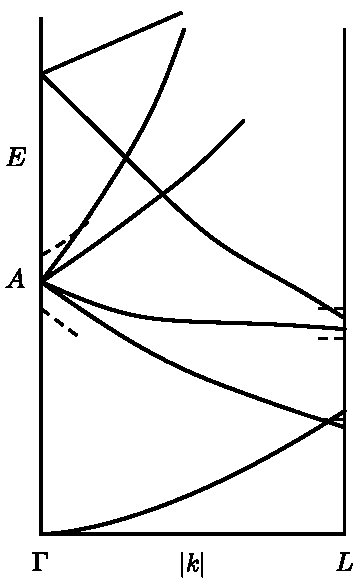
\includegraphics[width=0.66\textwidth]{fig_5.pdf}
\caption*{图 5　f.c.c. 空间格子沿从原点到区边界六边形面的直线（即 $k=(x,x,x)$ 方向）的能量对 $k$ 曲线（自由电子抛物面折回简约区后的结果）}
\end{figure}

\begin{center}
表 2

\begin{tabular}{clc}
\toprule
简并度 & 对称化平面波（S.P.W.） & 记号 \\
\midrule
$1$ & $\cos\dfrac{2\pi x}{a}\ \ \cos\dfrac{2\pi y}{a}\ \ \cos\dfrac{2\pi z}{a}$ & $\Gamma_1$ \\[4pt]
$1$ & $\sin\dfrac{2\pi x}{a}\ \ \sin\dfrac{2\pi y}{a}\ \ \sin\dfrac{2\pi z}{a}$ & $\Gamma_2$ \\[4pt]
$3$ & $\cos\dfrac{2\pi x}{a}\ \ \cos\dfrac{2\pi y}{a}\ \ \sin\dfrac{2\pi z}{a}$，等等 & $\Gamma_{15}$ \\[4pt]
$3$ & $\cos\dfrac{2\pi x}{a}\ \ \sin\dfrac{2\pi y}{a}\ \ \sin\dfrac{2\pi z}{a}$，等等 & $\Gamma'_{25}$ \\
\bottomrule
\end{tabular}
\end{center}

现在回到 Jones 区与布里渊区对比的问题。需要注意的一点是：二阶区边界处的能隙 $2V_K^{\mathrm{eff}}$ 很可能比一阶边界处的能隙小得多。因此，虽然我们一般预期每个边界处都有能隙，但在对称性复杂的情形下，特别大的能隙很可能只出现在真正的一阶边界处。这些边界就称为“Jones 区”的边界。以每原子态数来衡量的 Jones 区体积，与布里渊区的体积之间没有必然的联系；Jones 区只须每原子每自旋拥有某个有理数 $r>1$ 个态。例如，再回到众所周知的金刚石格子情形：第一布里渊区是一个胞，其区边界主要对应于 (111) $K$ 矢量，但该八面体的六个角尖被 (200) 边界切去。而在金刚石的 Jones 区中，八面体的角尖\emph{并未}被切去，这个胞每原子拥有 $9/8$ 个电子。

对特别重要的区边界的搜寻，可以超出寻找 $V\ne 0$ 的边界，进而扩展到那些 $V$ 特别大的边界。一般地，我们预期这样的边界乃是具有大 X 射线结构因子的边界，而后者只需察看 X 射线衍射花样便可简单地猜出（当然只当所有原子全同或近于全同时才如此，因为 X 射线与低能平面电子波所感受到的有效势颇为不同）。例如，金刚石中 (111) 的结构因子为
\begin{equation*}
F = 1 + \exp\left(\frac{3i}{2}\,\pi\right) = 1 - i,\qquad |F|^2 = 2
\end{equation*}
而对 $l+m+n=4N$（220、440、400 等）的那些晶面则为 $2$，$|F|^2=4$。这样看来，(220) 这一组晶面很可能围出一个特别重要的 Jones 区。

如果我们考察这一组倒格子矢量，就会认识到它们是一个棱长为 $4\times 2\pi/a$ 的面心立方倒格子的矢量；因此它也就是一个立方棱长为 $a/2$ 的体心格子的倒格子，原 f.c.c. 格子的每一个立方体对应于它的八个立方体。于是，由于b.c.c. 每个立方体只有 2 个原子而不是 4 个，这个格子的第一布里渊区对每个 f.c.c. 格子原子有 $8/2$ 即 4 个态，对每个金刚石格子原子有 2 个态——计入自旋总共 4 个。

看待这个准体心（pseudo-body-centered）格子的另一种方式，是把金刚石格子画出来，如图 6。

\begin{figure}[H]
\centering
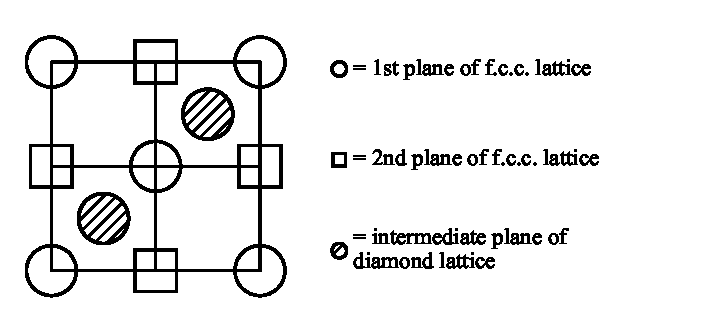
\includegraphics[width=0.6\textwidth]{fig_6.pdf}
\caption*{图 6　金刚石格子。$\circ$＝f.c.c. 格子的第一平面；$\square$＝f.c.c. 格子的第二平面；斜纹圆＝金刚石格子的中间平面}
\end{figure}

给出这些强反射的b.c.c. 格子可以这样得到：把每个原子周围四面体所缺的位置补齐，使之构成立方体，如图 7 中的圆圈 O 所示。

\begin{figure}[H]
\centering
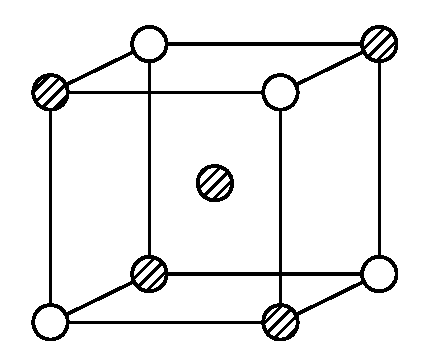
\includegraphics[width=0.6\textwidth]{fig_7.pdf}
\caption*{图 7　补全每个原子周围四面体的空缺位置（圆圈 O）以构成立方体，即给出强反射的b.c.c. 格子}
\end{figure}

这表明恰有两倍之多的态能装进它的布里渊区；在金刚石格子的强 Jones 区中，每个原子有四个电子态。

这一切都已被详细推演过，以此作为下述量子化学规则之半经验有效性的一个极好例证——正是这条规则赋予了 Jones 区重要性：晶体倾向于选择这样的结构，使得一个强的、对称的 Jones 区能够恰好或几乎恰好被填满。其理由很容易看出：如果晶体价带中的电子数使得在自由电子模型下费米面恰好会到达 Jones 区边界，那么该边界的形成就会降低区边界附近那群自由电子的能量——办法是使被占据的电子态相对于未被占据的态能量降低。

为了定量估计这一效应，设相应的 $V_K$ 的大小为 $V$。平均而言，粗略地说，能量在费米面附近 $V$ 范围内的每个电子，其能量都被降低了 $V/2$，于是降低量为 $(V^2/2)$ 乘以费米面处的态密度。在自由电子模型下，这个态密度由下式给出：
\begin{align*}
\text{每个电子的态密度} &= \frac{dn}{dE}\,\frac{1}{n} \\
&= \frac{dk}{dE}\left(\frac{1}{n}\,\frac{dn}{dk}\right) = \frac{dk}{dE}\,\frac{3}{k_F} \\
&= \frac{3}{2E_F}
\end{align*}
于是每原子的结合能将为
\begin{equation*}
\sim \frac{4\times 3}{2\times 2E_F}\,V^2 = \frac{3V^2}{E_F}
\end{equation*}
必须提醒读者，这一估计中的数值因子实际上不可能算得比数量级更准；事实上，有关这一情形的能量学目前在相当程度上仍有争议 (24)。

这一效应可能相当大，而且很可能正是它决定着晶体结构——只要在一些真实物质中估计一下它的影响便可以看出。例如，金刚石的自由电子费米能将是 30 ev（约 2 Rydberg），而在密度小得多的晶体 Si 和 Ge 中约为其一半。（这只须由 $n=k_F^3/3\pi^2$ 算出 $k_F$ 即可得到；结果金刚石的 $k_F$ 约为 $3\times 10^{8}\,\mathrm{cm}^{-1}$，Si 约为 $2\times 10^{8}\, \mathrm{cm}^{-1}$。）自由电子所感受到的势的各分量的实际数值，可从 Herman (23) 与 Phillips (25) 的计算中获得；它们给出：金刚石中 $V_{220}$ 约为 0.4 ryd，即 5 ev；Si 中约为 0.15--0.2 ryd，即 2 ev。于是内聚能的增益非常大：金刚石中为 3 伏特（译注：原文单位为 volts，此处即指电子伏），约占总内聚能的一半；Si 中为 1.5 伏特。诚然这是一个非常粗略的估计，但它表明，在决定一种物质将采取何种晶体结构的、通常相当微妙的能量平衡之中，这可能是一种真实而起支配作用的效应。

一个有趣的事实是：$K=111$ 的 $V_K$ 也在金刚石和硅的带隙附近扮演重要角色，它在某些 $V_{220}$ 无法起作用的对称点——尤其是 $\Gamma$ 点——处对打开带隙至关重要。因此，对结合能的一个可观贡献也来自 $V_{111}$。这大概是几个因素的组合决定了所观察到的晶体结构的一个典型例子。

在转向更定量的内容之前，我想从这一粗略计算中引出若干物理与化学上的教益。首先，注意我们在这里为开放型、价型（valence-type）结构看到了一个物理上的理由，它完全摆脱了把定向键设想为从原子沿确定方向伸出的若干小棍棒的观念。在一个多价物质中，开放结构完全可以只是一种手段，把重要的 Jones 区边界带进费米面所处的区域。不过我应当提醒读者：作为一件化学事实，键的方向性看来确实存在；而且，一个给定物质究竟会采取具有大致正确的密度与 Jones 区形状的哪一个具体结构，其计算很可能是 $V$ 的极多傅里叶分量之间复杂相互作用的问题。眼下这通常最好留给行之有效的半经验方法与化学直觉去处理；但我们至少看到了其中涉及的某些原理，而且这些原理并不像 Pauling 可能会提示的那样，要求抛弃能带理论这套非常成功的工具。

其次，注意在这两种情形中，$V$ 实际上都小到使微扰论并不太差的程度。对金刚石来说这是相当令人吃惊的，但却是事实——金刚石巨大的能隙只是碳的整个能量标度很宽这一事实的后果，并不代表对近自由电子图像的真正大的偏离。

最后，我应当提到，这个对金刚石和硅的应用实际上是这类应用中最新的一个；历史悠久得多、研究也彻底得多的领域，是把它应用于某些合金结构——或者更确切地说，金属间化合物结构——特别是著名的 Hume-Rothery 合金。欲知较好的论述，可参见 Jones (26)。这些化合物具有各种多少有些复杂的立方结构，往往有一个对称性相当高的突出 Jones 区位于非常靠近费米面之处。它们无疑是由同样的效应引起的，但毫无疑问，其能量贡献比价结构中的要小得多。我们看到这一点的依据是：这些化合物仍保持其金属性，表明区边界并未打开多大的能隙。还值得强调的是，即使在例如金刚石的情形中，某些特殊的对称方向——即 Jones 区的角点，按对称性它们等价于简约区的中心 $\Gamma$——在近自由图像中也无法仅由 $V_{220}$ 这一个分量使之劈裂，因此 $V$ 的其他分量，特别是我们前面提到的 $V_{111}$，在打开造成绝缘行为的实际能隙方面起着支配作用。

% 衔接说明：p058 页首即本小节标题，其上无前节残句，本文件自标题起译。

\subsection{元胞法：结合能的定量计算}

这是一种完全不同的方法；在许多方面，它都已证明是计算金属内聚能（cohesive energy）迄今为止最为准确的方法。元胞法（cellular method）由 Wigner 和 Seitz 首先采用，可惜由于种种已知的原因，它似乎只容易应用于单价碱金属。

元胞法在几乎每一个可能的方面都与基于平面波的方法形成对照。在近自由电子模型中，以及我们将会看到的、在 O.P.W.（正交化平面波）方法中，波函数从一开始就被选为恰当的能带函数，满足晶格周期性所强加的边界条件；随后的功夫则在于用微扰或其他方法足够精确地处理离子实（ion cores）的势对这些函数产生的效应。元胞法却是从相反的尝试出发：先在离子实区域求出尽可能精确的势和尽可能精确的解，然后再去近似地满足由周期性所强制的边界条件。看来，在计算能量时这是更为精确的途径，但它只是对固体 s 带中最低的波函数才是如此。

具体做法是把实空间格子划分成元胞，方式与在倒格子中构成布里渊区的做法完全相同：对指向近邻的矢量作平分。对于碱金属通常被假定具有的 b.c.c. 格子，这样得到的是由 $\tfrac{1}{2}\,\tfrac{1}{2}\,\tfrac{1}{2}$ 平面构成的正八面体，其角被 $\tfrac{1}{2}\,00$ 平面切去——总共 14 个面——正是我们已经熟悉的那种多面体。元胞法的想法是：这个多面体其实同球相去不远，而且在发生偏离的外部区域，势非常弱、波函数非常平滑。于是就作出了元胞严格为球的近似。这使得对低态数值积分波动方程的问题得到如下若干简化：

1. 格子的其余部分也不妨同样假定是球对称的；由于碱金属中原子间的距离使得离子实几乎不发生交叠，来自其他元胞的势纯粹是静电势，而在这个假定下它完全消失，因为格子整体是中性的。

2. 再者，原子芯是闭合壳层，因而是球形的；结果我们在元胞内要求解的乃是一个球对称的——即完全可分离的——波动方程。

3. 对于 s 带的最低态——它当然 $k=0$，因而其波函数是简单周期的，即 $u_0(r)$——边界条件取如下简单形式：斜率 $\mathrm{d}\psi/\mathrm{d}r\,\big|_{r=R_{\mathrm{cell}}}=0$。这是因为波函数必须水平地趋近元胞边界，因为根据反射对称性，它必须关于边界为偶。最低的原子态则是 $\mathrm{d}\psi/\mathrm{d}r\,\big|_{r=\infty}=0$ 的那个球对称态。碱金属内聚、而且实际上也就是所谓“金属键”的根本物理基础在于：$\mathrm{d}\psi/\mathrm{d}r\,\big|_{r=R_c}=0$ 的态，其能量比自由原子中态的能量低相当多。Wigner 称之为“边界修正”（boundary correction），并在他的《Seitzschrift》文章 (25) 中对多种金属作了估计。

从相当粗略的考虑出发，我们立刻就能看出必然如此。球对称性使我们能够把波动方程 $-\nabla^2\Psi+V(r)\Psi=E\Psi$ 分离成角向方程和径向方程，只须假定 $\Psi=[U_L(r)/r]\,Y_{LM}(\theta,\phi)$；于是 $U_L$ 满足的方程是
\begin{equation*}
\frac{d^2 U_L}{dr^2}+\left[E-V(r)-\frac{L(L+1)}{r^2}\right]U_L=0
\end{equation*}
这里的单位是原子单位：$r$ 以玻尔半径计，所有能量以 rydberg 计。在碱金属原子的芯区之外，$V=-2Z/r$，在单价原子的情形即 $-2/r$；芯内的 $V$ 则更为复杂，而且实际上并不是一个局域算符，还包含与芯电子的交换。尽管如此，为了定性的目的，我们可以把它当作一个纯势 $-2Z(r)/r$ 来处理（图 8）。

\begin{figure}[H]
\centering
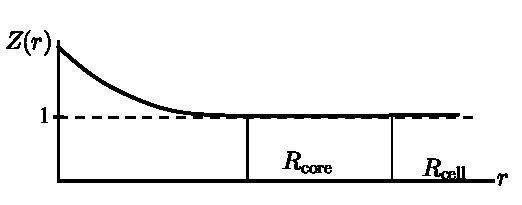
\includegraphics[width=0.72\textwidth]{fig_8.pdf}
\caption*{图 8}
\end{figure}

我们感兴趣的是低的 s 态（$L=0$），于是在 $r=0$ 处的边界条件是 $\Psi$ 有限，即 $U=0$ 且线性增大。让我们取某个很低的能量 $E_1$，在想象中从原点处这一边界条件出发把方程向外积分。在到达 $R_t(E_1)$ 处的“经典转折点”（classical turning point）之前，$E_1-V>0$，$\mathrm{d}^2U/\mathrm{d}r^2$ 与 $U$ 反号，曲率朝向轴；然而此后，$U>0$，$\mathrm{d}^2U/\mathrm{d}r^2>0$，曲率背离轴：$U$ 发散。现在让我们依次画出能量递增的 $E_1$、$E_2$、$E_3$ 以及 $E_f$——实际的自由原子本征值——的情形。我们看到，自由原子本征值高于使波函数在 $R_{\mathrm{cell}}$ 处恰好变平的那个能量；在此之后，波函数便转而增大并发散（图 9）。由此得到的动能收益可以相当可观。以钠为例，它是 3 1/2 伏特（译注：原文单位为 volts，此处即指电子伏）；在 Li 中更高，在重碱金属 K、Rb 和 Cs 中则更低。

\begin{figure}[H]
\centering
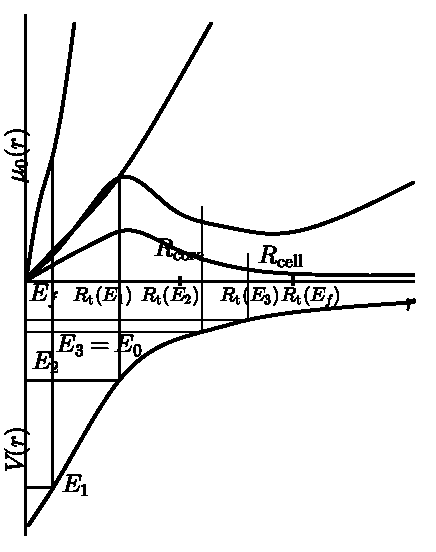
\includegraphics[width=0.72\textwidth]{fig_9.pdf}
\caption*{图 9}
\end{figure}

从这幅图出发，还可以对 Kuhn、Van Vleck、Brooks (21) 和 Ham (18) 为计算这一能量而发展的既精确又巧妙的方法获得相当好的了解。在两幅图中，我都标明了一个对所有碱金属都成立的事实：芯轨道（Li 中的 1s、Na 中的 2s2p，等等）的尺度比原子元胞小得多。这意味着在径向积分中存在一段相当可观的区域，在其中我们确切知道必须使用的势，即 $V=-2/r$。当然，芯内的势是未知的；在较早的计算中，对这一区域的做法是先取一个 Hartree 或 Hartree-Fock 势，然后修改它，使之拟合观测到的光谱项值序列——对碱金属原子，这些项值已为人们以极高的精度所知。

Kuhn 和 Van Vleck 指出，事实上也许永远不必穿过这一区域去积分径向方程。既然反正要使用一组取自光学光谱的经验能级来调整势，难道就不能有办法直接从光学光谱本身提取必要的信息吗？

Kuhn-Van Vleck 方法在原理上比 Brooks 和 Ham 最终完成的更精确、更完备的技术要简单。他们的做法是：把波函数看作从 $R=0$ 处 $U=0$ 出发、一直积分到 $R_{\mathrm{core}}$ 点的结果。在该点上，要把积分继续下去所需的全部信息就是对数导数（logarithmic derivative）$(1/U)(\mathrm{d}U/\mathrm{d}r)\,\big|_{r=R_{\mathrm{core}}}$。这个数将是初始能量 $E$ 的某种函数；如我们所见，对大的负 $E$，它从某个高值出发，下降穿过零，最后变得像一条 $\cot^{-1}$ 曲线。从 $R_{\mathrm{core}}$ 点往外，我们确切地知道势具有 $(-2/r)$ 的形式，而 Wannier 等人已经求出了任意能量下这两个解的解析形式。于是，我们可以把这些解拟合到

\begin{figure}[H]
\centering
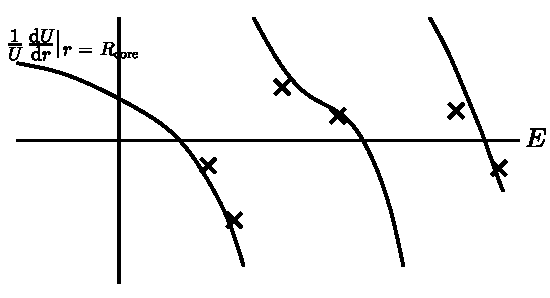
\includegraphics[width=0.6\textwidth]{fig_10.pdf}
\caption*{图 10}
\end{figure}

任意给定的 $(1/U)(\mathrm{d}U/\mathrm{d}r)$ 值，并确定解在任意能量下的性质。特别地，我们能解析地定出那些可以导致 $\mathrm{d}U/\mathrm{d}r\,\big|_{r\to\infty}=0$ 的 $(1/U)(\mathrm{d}U/\mathrm{d}r)\,\big|_{R_{\mathrm{core}}}$ 值；它们就是观测到的光谱项能量处的值。随后我们就可以把这些值描绘出来；图 10 中的那些 $x$ 就是一组假想的值。在大致知道曲线应有的形状之后，我们可以试着过这些给定的点画一条光滑曲线，并假定它就是正确的 $(1/U)(\mathrm{d}U/\mathrm{d}r)\,\big|_{r=R_c}(E)$。

我们还能解析地知道——这同样是因为我们掌握着库仑波方程解的精确解析行为——$(1/U)(\mathrm{d}U/\mathrm{d}r)\,\big|_{R_{\mathrm{core}}}$ 取什么值才会导致 $(1/U)(\mathrm{d}U/\mathrm{d}r)\,\big|_{R_{\mathrm{cell}}}=0$。把这个值记作 $(1/U)(\mathrm{d}U/\mathrm{d}r)\,\big|_0$。然后只须把我们的光滑曲线内插到这个值，便得到最低本征值的数值 $E_0$。

事实上，由于对数导数曲线的形状相当难以驾驭，它并\emph{不}是应当描绘的正确量；正如 Kuhn 本人首先指出的，能给出真正光滑外推的正确量是\emph{量子亏损}（quantum defect），它在自由原子本征值处正是碱金属光谱的 Ritz 内插公式中的量 $\delta_m$，
\begin{equation*}
E_m=-\frac{1}{(m-\delta_m)^2}
\end{equation*}
$\delta_m$ 与碰撞理论中出现的相移 $\delta$ 密切相关，不过库仑势的长程性质引入了一些除专家以外无人感兴趣的额外复杂因素。无论如何，人们发现——而且可以在数学上加以证明——总能找到一个量 $\delta$，它在观测到的光谱系各项之间光滑地内插，并且可用来满足元胞表面上任意希望的边界条件。在 Ham 的文章中，对五种碱金属各自的若干种密度，以三到四位有效数字给出了相应的 $k=0$ 能量。

这种方法的主要优点——这也可能是大多数内聚能计算（以别于实际能带形状的计算）用其他方法之所以不成功的最重要的原因之一——在于：价电子与芯电子相互作用中的多体效应，基本上被精确地包含在所使用的量子亏损经验值之中。甚至有可能在 $R_{\mathrm{core}}$ 之内根本不存在任何合理的局域势 $V(r)$ 能给出观测到的本征值谱；正如我们提到过的，即使在 H-F 中，正确的势也是非局域的。这看来实际上就是如下情形的主要原因：早期的 Wigner-Seitz 计算对 Li 和 Na 相当好，对 K 相当差，对 Rb 和 Cs 则根本行不通，而 Q.D.M.（量子亏损方法）对付重金属却毫无困难——在重金属中，由于芯更大、束缚更松，芯极化（core polarization）与交换都是很大的效应。

于是，$k=0$ 处那单独一条能级的定位，由 Q.D.-元胞法做得极为出色；这也正是它胜过所有其他方法的地方：至少有一条能级可以按绝对值准确定位。尽管如此，这还不可能是全部的战斗；我们必须首先计入所谓的“费米能”，即由于其余电子不得不进入带中较高的状态而出现的额外动能。接着，我们还必须对电子相互作用作一组相当大的修正；不过，这些修正之和结果证明相当小。

费米能是一个相当大的效应，从 Wigner 的定性论证 (20) 看得很清楚：该论证提示，一个 s 带被完全填满的物质将几乎是不结合的。从积分径向方程的观点看，带顶的状态必须是那种从原子到其近邻改变符号的状态，这意味着 $\psi$ 在 $R_{\mathrm{cell}}$ 处为零，而不是 $\mathrm{d}\psi/\mathrm{d}r$ 在 $R_c$ 处为零。$\psi=0$ 的波函数，其能量比自由原子波函数 $E_I$ 的能量所高出的量，大概与 $E_0$ 比 $E_I$ 低的量大致相同。可以看到，在某种意义上，$\psi$ 在 $\infty$ 处趋于 0 大致是 $\psi\big|_{R_c}=0$ 与 $\mathrm{d}\psi/\mathrm{d}R\,\big|_{R_c}=0$ 之间的一个中间判据（图 11）。于是，对半满的带，我们或许会预期在费米能上损失掉 $k=0$ 态所赢得的 3 到 4 伏特能量的一半或更多，而事实证明确实如此。

\begin{figure}[H]
\centering
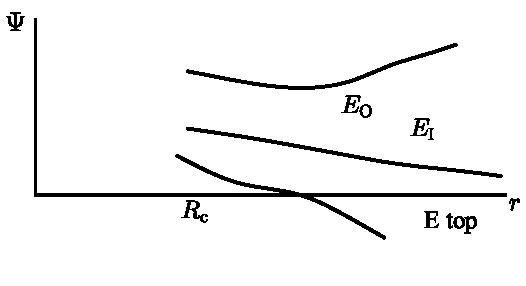
\includegraphics[width=0.72\textwidth]{fig_11.pdf}
\caption*{图 11}
\end{figure}

要计算费米能，就必须对 $k$ 空间中整个被占据区域的能带结构有相当准确的估计。结果表明，用元胞法时，对第一区边界附近的点、或者对波函数在元胞内不再呈 s 型的较高的带，这是一种困难而且常常不准确的计算。原因在于，元胞内波动方程的解正是角动量 $L=0,1,2$ 等等的 $s$、$p$、$d$ 等本征函数。……随着 $L$ 增大，计算或外推的精度迅速下降，因此，对 $L\geq 3$ 或 4 的波函数拟合规定的边界条件是非常困难的事情。这是由于有效排斥势能 $L(L+1)/r^2$ 的存在——在相应的光学能级中，它把电子挡在芯区之外；而固体问题中作边值拟合所需的波函数却确实穿透到芯区。

结果证明，遗憾的是，对相当大的 $k$，能带波函数包含非常可观的一些成分，必须用高角动量值的波函数才能描述。看到这一点的最简易途径是 Shockley 的“空晶格”（empty lattice）检验——我们可以把对称化平面波（它们是能带波函数的一个可能的集合）绕元胞中心按球谐函数展开，而且的确发现，对接近或越过区边界的那些 $k$ 值，它们含有相当可观的 $L\geq 3$ 或 4 的分量。尽管在把球谐函数拟合到正确边界条件这一数学问题上已经取得进展，但对碱金属以外的一切金属，其精度仍属可疑。

当然，对碱金属而言这个问题并不十分严重，因为很大一部分电子的 $k$ 值深处于第一区之内。这里使用的技巧是把能量 $E(k)$ 在原点附近按 $k$ 的幂级数展开；由对称性，第一项为零，第二项即所谓的有效质量（effective mass）项，
\begin{equation*}
E=E_0+\frac{\hbar^2 k^2}{2m^*}+\cdots
\end{equation*}
则可以用“$k\cdot p$”微扰论的一个计算求得。这种方法的原理是：写出并非由总波函数 $\psi_k(r)$、而是仅由其周期部分 $u_k$ 所满足的波动方程。我们从通常的波动方程
\begin{equation*}
\left[-\frac{\hbar^2}{2m}\nabla^2+V(r)\right]u_k(r)\,e^{ik\cdot r}=E_k\,u_k\,e^{ik\cdot r}
\end{equation*}
出发。显然，除 $\nabla^2$ 之外的一切都与 $e^{ik\cdot r}$ 对易，因此在完成如下的计算之后，指数因子便可以提出来：
\begin{align*}
\nabla^2\left(u_k\,e^{ik\cdot r}\right)&=\nabla\cdot\left(\nabla u_k+ik\,u_k\,e^{ik\cdot r}\right)\\
&=-k^2 u_k\,e^{ik\cdot r}+2ik\,e^{ik\cdot r}\cdot\nabla u_k+\left(\nabla^2 u_k\right)e^{ik\cdot r}
\end{align*}
于是
\begin{equation*}
-\frac{\hbar^2}{2m}\left(\nabla^2+2ik\cdot\nabla\right)u_k+V(r)\,u_k=\left(E_k-\frac{\hbar^2 k^2}{2m}\right)u_k
\end{equation*}
当我们把它与本征函数 $\psi_0=u_0$ 所满足的方程
\begin{equation*}
-\frac{\hbar^2}{2m}\nabla^2 u_0+V(r)\,u_0=E_0\,u_0
\end{equation*}
相比较时，我们看到，除了
\begin{equation*}
-i\,\frac{\hbar^2}{m}\,k\cdot\nabla u_k=\frac{\hbar}{m}\,k\cdot p\,u_k
\end{equation*}
这一项之外，它就是同一个方程，而且由于 $u_k$ 是周期的，还具有相同的边界条件。于是，对足够小的 $k$，我们可以把这一项当作微扰来处理，从而得到用 $k=0$ 处的解表出的 $k$ 处能量的表达式。事实上，只须稍加修改，这个表达式就可以在任意一般点 $k_0$ 处使用，以求出邻近点上的波函数与本征值。

在我们所讨论的碱金属这一特殊情形中，$k\cdot p$ 项含有梯度算符，因而把偶函数变为奇函数，反之亦然。这意味着对角矩阵元 $(u_{0n},\,(k\cdot p)\,u_{0n})$ 为零，所以一级修正为零。二级修正按标准微扰论为
\begin{equation*}
E_k-\left(\frac{\hbar^2 k^2}{2m}+E_0\right)=-\frac{\hbar^2 k^2}{m^2}\sum_n\frac{|(0n|p_x|00)|^2}{E_n(0)-E_0}
\end{equation*}
于是
\begin{equation*}
\frac{1}{m^*}=\frac{1}{m}\left[1-\frac{2}{m}\sum_n\frac{|(0n|p_x|00)|^2}{E_n(0)-E_0}\right]
\end{equation*}
乍看之下，有效质量似乎总应增大——能带变得更为平坦——因为右边的求和预期 $>0$，其中 $E_n>E_0$。对 Li 来说确实如此：在 Li 中不存在低于价带的 $p$ 带（由于 $p_x$ 是矢量，所有重要的矩阵元都是到 $p$ 带的）；但一般而言未必如此，而且事实上在其余碱金属中——可能 Na 除外——情形都不是如此。因此，到那些代表闭合壳层的带的矩阵元就相当重要。

虽然 Wigner 和 Seitz 的原始计算直接使用了 $k\cdot p$ 理论，但 Bardeen (27) 很快就引入了一个简单得多也精确得多的程序，他注意到波函数的一级修正可以基本上精确地算出。做法是直接迭代波动方程，即从展开
\begin{equation*}
u_k=u_0(r)+u_1^{\,k}(r)+\cdots
\end{equation*}
出发，于是有
\begin{equation*}
\left(-\frac{\hbar^2}{2m}\nabla^2+V-E_0\right)u_1=\frac{i\hbar^2}{m}\,k\cdot\nabla u_0
\end{equation*}
他观察到，$u_1$ 的一个特解是
\begin{equation*}
u_1^{(a)}=-i\,k\cdot r\,u_0(r)
\end{equation*}
（代入即可验证；非齐次项与 $\nabla(k\cdot r)\cdot\nabla u_0$ 项正好相消）。但它并不满足边界条件；这个边界条件显然是（因为 $u_1$ 应当具有 $p$ 函数的对称性并且是周期的）：解在元胞边界上为零。

我们可以在该解上加上齐次方程的一个 $p$ 函数解，使之在元胞边界上为零：
\begin{equation*}
V_1=\frac{i\,k\cdot r}{r^2}\,P(r)
\end{equation*}
其中 $P$ 是径向波动方程在固定能量 $E_0$ 下的一个解：
\begin{equation*}
\frac{d^2 P}{dr^2}-\frac{2}{r^2}\,P(r)+\frac{2m}{\hbar^2}\,(E_0-V)\,P=0
\end{equation*}
于是
\begin{equation*}
u_1=i\,k\cdot r\left(P/r^2-u_0(r)\right)
\end{equation*}
这样
\begin{equation*}
\left.\frac{P}{r^2}\right|_{R_c}=\left.u_0\right|_{R_c}
\end{equation*}

我们立刻认识到，量子亏损方法（quantum-defect method）的设置正是为了直接给我们——通过从 $p$ 态的光学光谱作内插——波函数 $P(r)$ 的一切有趣的性质，至少在元胞的外部部分是如此。通过运用一系列巧妙的变换，Bardeen 得以把二级能量修正完全用波函数的这个一级修正表示出来，甚至还用它在元胞边界处的行为表示出来：
\begin{equation*}
\alpha=\frac{m}{m^*}=\gamma\left[\frac{r}{P}\,\frac{dP}{dr}-1\right]_{R_c}
\end{equation*}
而
\begin{equation*}
\gamma=-\frac{1}{3}\,R_c\,\bigl[u_0(R_c)\bigr]^2\Bigg/\left[\gamma\,u_0(r)\,\frac{d}{dr}\left(\frac{1}{r}\,\frac{\partial u_0}{\partial E}\right)\right]_{R_0,\,E_0}
\end{equation*}
（译注：此式分母中的 $\gamma$ 与求值下标 $R_0$ 均按原书排印照录。）这个证明（部分归功于 Silverman 等人）相当冗长，所以我不打算在这里讨论。

在所有碱金属中，微扰论都收敛得相当好，因为 $u_0$ 相当平滑（微扰即 $\alpha(k\cdot\nabla)u_0$）。在 Na 中，$u_0$ 在元胞 90\% 的范围内几乎是个常数。于是，动能修正亦即费米修正 $E_F$ 恰好就是自由电子气的那个值，再对修改后的有效质量加以改正。它就是
\begin{equation*}
\int_0^{k_f} k^2\,dk\,\frac{\hbar^2 k^2}{2m^*}\Bigg/\int_0^{k_f} k^2\,dk=\frac{3}{10}\,\frac{\hbar^2 k_F^{\,2}}{m^*}
\end{equation*}
其中 $k_F$ 由下式确定：
\begin{equation*}
n=\frac{k_F^{\,3}}{3\pi^2}
\end{equation*}
这可以写成
\begin{equation*}
E_F=\frac{2.21}{r_s^{\,2}}\left(\frac{m}{m^*}\right)\quad\mathrm{ryd}
\end{equation*}
其中
\begin{equation*}
\frac{4\pi}{3}\,a_0^{\,3}\,r_s^{\,3}=\frac{1}{n}
\end{equation*}
对若干种碱金属给出各种相关的量（见表 3），会使我们对各种效应的数量级有一个感受。

% 注：p067 末句完整结束；其后正文所引“表 3”的表体在后续页，由下一文件处理。

% ---- B.2 收尾：表 3 与讨论段（原书 p.53 / PDF p068 顶部，协调者补译） ----
\begin{table}[H]
\centering
{\bfseries 表~3}\\[6pt]
\small
\setlength{\tabcolsep}{4.5pt}
\renewcommand{\arraystretch}{1.25}
\begin{tabular}{@{}llllllll@{}}
\toprule
元素 & $r_s$ & $-E_0$ & \shortstack{内聚边界修正\\$E_I-E_0$\ensuremath{,} ev}
 & \shortstack{动能修正\\$m/m^*$} & $E_F$\ensuremath{,} ev
 & \shortstack{未修正内聚能\\$E_I-E_0-E_F$\ensuremath{,} ev}
 & \shortstack{观测内聚能\\ev}\\
\midrule
Li & 3.21 & \shortstack[r]{0.69 ryd =\\9.4 ev} & 4.0 & 0.67 & 1.90 & 2.10 & 1.65\\
Na & 3.96 & \shortstack[r]{0.625 ryd =\\8.5 ev} & 3.15 & 1.02 & 2.0 & 1.15 & 1.20\\
Rb & 5.20 & 6.27 ev & 1.65 & 1.10 & 1.23 & 0.42 & 0.85\\
\bottomrule
\end{tabular}
\end{table}

这张表足以显示各种结果的大致面貌。正如我们所猜想的，Fermi 动能修正大致达到边界修正的二分之一到三分之二，而二者的差在数量级上给出金属的结合能。注意，内聚能是问题中最小的能量——它是作为大得多的数字之差被算出来的——这几乎总是如此，也正是结合能计算中困难的主要根源。把能带算准到 0.1 ryd 左右并不难，这对了解能带结构的一般面貌通常已令人满意，因为能带结构的尺度往往是 rydberg 量级，至少也是 0.4 到 0.5 ryd；但结合能却是 0.1 或更小。

\subsection{自由电子气中的交换与关联}

写到这里，各位也许会有一点惊讶：我们竟然已经非常接近于算出真实的结合能了。你完全有理由发问：金属电子自身的 Coulomb 相互作用又怎么样了呢？表面看来，我们把这些完全忽略了，因为在计算波函数时我们只用了离子实的场。

实际上，价电子之间的相互作用已在很大程度上以一种非常巧妙而不动声色的方式考虑了进来。Wigner 所做的，实质上是把价电子处于不同原子上时的相互作用包括了进来，因为他让近邻的元胞呈电中性，而不像\emph{只}有离子实存在时那样带 $+1$ 电荷；但他有意略去了同一元胞内电子之间的相互作用。对于交换（exchange）与关联（correlation）效应而言，这是一个十分合理的近似。先说交换——我们知道，不相容原理会在一个给定电子周围的自旋平行电子分布中挖出一个“空穴”。Coulomb 排斥则倾向于把自旋反平行的电子也从给定电子的邻域排开，于是净效果是：从该电荷的邻域中大约移走了整整一个电子的电荷。这个空穴的半径为 $r_s$ 的量级，因此在计算波函数时，不妨当作每个元胞内在同一时刻只允许存在一个电子来处理。结果是：无须求解任何非常复杂的波动方程，我们所处理的波函数就已经算到了实际上与 Hartree-Fock 相当的精度。在多价金属中这种空穴相对较小、因而这一近似不再适用——这一事实也许是在此类金属中结合能计算困难的另一个原因。

尽管如此，为了得到真正精确的最终答案，关键还是要回到这些波函数，并尝试对“多体”修正作出更完备的估计。基于上述理由，我们预期所有这些修正之和接近于零，但各个单项却会相当大。

使 Wigner 和 Seitz (28, 29) 能够对这些项作出良好估计的，是一个幸运的事实：碱金属中的电子，除了那个使总能量整体下降的常数“边界修正”之外，其行为非常像一团真正自由的电子气体。如前所述，在 Na 中，在元胞体积的 90\% 以上的区域内，波函数实际上就是 $e^{i\mathbf{k}\cdot\mathbf{r}}$。这使得我们可以使用自由电子气自相互作用能的理论。而这一理论由于气体必须在空间中“均匀”这一事实而大为简化——也就是说，它在空间每一点处的性质必须相同。

人们最先施加的修正是 Hartree 修正，即所有电子的平均场。在自由电子的情形下，它是整个均匀电荷分布的自相互作用能，并按 $v^{2/3}$ 发散；当然，这一发散必定会被来自离子电荷的一个等值反号的项所抵消，正是后者保证了电中性。研究自由电子气时，通常的做法是完全忽略这一项：人们用一团均匀的正电荷“果冻”（jelly）来代替离子实，它恰好抵消自由电子的平均电荷。

而在真实的碱金属中，情况则不同：确实存在这样一项，而且事实上相对于内聚能它还是大的。我们此前已把与中心电荷球以外一切的相互作用包括了进来，所以还必须把一个电荷为 $e$、半径为 $R_{\mathrm{cell}} = r_s a_0$ 的球的 Coulomb 自能包括进来，它等于 $3e^2/5R_c = 6/5r_s$ ryd。如你所见，在 Li 中这超过了 4 伏特，足以把全部符合都破坏掉。

为了与这一项相抗衡，我们必须计算那两种倾向于使电子彼此分开的效应：交换本身，以及关联。后一种能量的定义相当人为：它是最优的 Hartree-Fock 解与正确的解之间的能量差。我们不打算在这里计算关联能（correlation energy），但交换效应我们能够处理；而且，由于其数学与思想日后对我们有用，我们也就来做这件事。

注意到在自由电子气的情形下 Hartree 项只是一个平庸的常数，包含交换的 H-F 方程即为
\begin{equation*}
-\frac{\hbar^2}{2m}\,\nabla^2\phi_{k\sigma} - \sum_{k'\ \mathrm{occ}} \int \mathrm{d}\mathbf{r}'\ \phi^*_{k'\sigma}(\mathbf{r}')\,\phi_{k\sigma}(\mathbf{r}')\,\frac{1}{|\mathbf{r}-\mathbf{r}'|}\,\phi_{k'\sigma}(\mathbf{r}) = E_k\,\phi_{k\sigma}(\mathbf{r})
\end{equation*}
由于系统作为一个整体仍具有平移对称性，通过假设
\begin{equation*}
\phi_k = \frac{1}{\sqrt{V}}\,e^{i\mathbf{k}\cdot\mathbf{r}}
\end{equation*}
便可以得到一个自洽解——即便它不一定就是最低的解。于是交换项变为
\begin{equation*}
A\phi_k(\mathbf{r}) = \int \mathrm{d}\mathbf{r}'\ A(\mathbf{r},\mathbf{r}')\,\phi_k(\mathbf{r}')
\end{equation*}
\begin{align*}
A(\mathbf{r},\mathbf{r}') &= \sum_{k'}\frac{e^2}{|\mathbf{r}-\mathbf{r}'|}\,\phi^*_{k'}(\mathbf{r}')\,\phi_{k'}(\mathbf{r})\\
&= \frac{e^2}{V}\sum_{k'}\frac{e^{i\mathbf{k}'\cdot(\mathbf{r}-\mathbf{r}')}}{|\mathbf{r}-\mathbf{r}'|} = A(\mathbf{r}-\mathbf{r}')
\end{align*}
这确实具有平移对称性（不依赖于 $\mathbf{r}+\mathbf{r}'$），因此方程的解的确可以是平面波。

我们实际上能够把 $A(\mathbf{r}-\mathbf{r}')$ 的形式计算出来；它常被称作交换空穴（exchange hole）的势。这一推导的大部分应归功于 Dirac (30)。我们可以把它看作围绕 $\mathbf{r}'$ 处电子的电荷分布中一个“空穴”所产生的势：
\begin{align*}
\rho(\mathbf{r}-\mathbf{r}') &= \frac{e}{V}\sum_{k\ \mathrm{occ}} e^{i\mathbf{k}\cdot(\mathbf{r}-\mathbf{r}')}\\
&= \frac{e}{V}\left(\frac{n}{2}V\right) \frac{\displaystyle \int_0^{k_F} k^2\,\mathrm{d}k \int_{-1}^{1}\mathrm{d}x\ e^{ik|\mathbf{r}-\mathbf{r}'|x}}{\displaystyle 2\int_0^{k_F} k^2\,\mathrm{d}k}
\end{align*}
利用
\begin{equation*}
\frac{n}{2} = \frac{4\pi}{3}\,\frac{k_F^3}{8\pi^3} = \frac{k_F^3}{6\pi^2}
\end{equation*}
并令 $R = |\mathbf{r}-\mathbf{r}'|$，它就是
% 校注：原书此处两处分母均印作 2\pi^2 R；按本节自洽性（下文 A(R) =
% e^2 k_F^4/2\pi^2[...]，以及精确核 A = (e^2/V)\sum e^{ik·R}/R），
% 分母应为 2\pi^2 R^2，此处按本意转写。
\begin{equation*}
= -\frac{e^2}{2\pi^2 R^2}\,\frac{\mathrm{d}}{\mathrm{d}R}\left\{\int_0^{k_F} \cos kR\ \mathrm{d}k\right\} = -\frac{e^2}{2\pi^2 R^2}\,\frac{\mathrm{d}}{\mathrm{d}R}\left(\frac{\sin k_F R}{R}\right)
\end{equation*}
\begin{align*}
&\left(\text{因为当 } k \to 0 \text{ 时 } \frac{\sin kR}{R} \to 0\right)\\
% 校注：原书前置因子印作 e k_F/2\pi（放大核查确无上标）；但由 \rho(0)=en/2
% （图 12 中水平线标记 n/2 = e k_F^3/6\pi^2，曲线自零出发）以及正文陈述
% A = e\rho/R（与下式 A(R) 精确一致），前置因子应为 e k_F^3/2\pi^2，
% 此处按本意转写。
\rho(R) &= \frac{e k_F^3}{2\pi^2}\left[-\frac{\cos k_F R}{(k_F R)^2} + \frac{\sin k_F R}{(k_F R)^3}\right]
\end{align*}
图 12 给出了交换空穴的图像。（注意在 $R = 0$ 处诸奇性相互抵消。）图中画出的是：一个位于零点的电子在 $R$ 处所看到的自旋平行电子的总有效密度。

\begin{figure}[H]
\centering
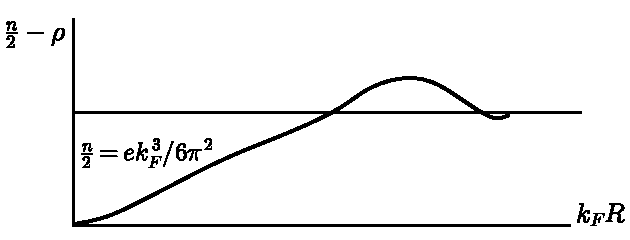
\includegraphics[width=0.72\textwidth]{fig_12.pdf}
\caption*{图 12　交换空穴：位于原点的电子周围自旋平行电子的总有效密度 $n/2-\rho$ 随 $k_F R$ 的变化，水平线标记 $n/2 = ek_F^3/6\pi^2$（原书图注仅作 “Figure 12”）}
\end{figure}

相应的核——交换势 $A(\mathbf{r}-\mathbf{r}')$——当然就是 $e\rho$ 除以 $R = \mathbf{r}-\mathbf{r}'$：
\begin{equation*}
A(R) = \frac{e^2 k_F^4}{2\pi^2}\left(\frac{\sin k_F R}{(k_F R)^4} - \frac{\cos k_F R}{(k_F R)^3}\right)
\end{equation*}

这些函数带着它们在无穷远处特有的甚长程振荡行为，在自由电子气理论中极其常见也极其有用。$A$ 类似于自由电子气的“Green 函数”，而熟悉自旋共振的读者会在 $A(\mathbf{r})$ 中认出 Ruderman-Kittel 函数。这种长程的振荡行为，是对费米分布的积分中存在尖锐上限的结果，而且只有在存在自由费米面时才会出现。这两个函数包含的是 $2k_F R$ 而非 $k_F R$，因为它们来自一个稍有不同的积分，但振荡的缘由是相同的。

一个给定平面波态 $k$ 的能量中的交换贡献，很容易由
\begin{equation*}
A\phi_k(\mathbf{r}) = \int A(\mathbf{r}-\mathbf{r}')\,\phi_k(\mathbf{r}')\ \mathrm{d}\mathbf{r}'
\end{equation*}
导出。根据对 Fourier 变换作折叠的卷积定理（convolution theorem），它就是
\begin{equation*}
A\phi_k = A_k\phi_k
\end{equation*}
其中
\begin{equation*}
A_k = \int \mathrm{d}\mathbf{R}\ e^{i\mathbf{k}\cdot\mathbf{R}}\,A(R)
\end{equation*}
这个 Fourier 变换可以直接计算，也可以按下面的办法来做：$A(\mathbf{r}) = \rho(\mathbf{r})/r$，于是再次利用卷积定理，
% 校注：原书此行被积函数印作 \rho(k)；按卷积定理并对照下一行应为 \rho(k')，
% 此处按本意转写。
\begin{align*}
A_k &= \frac{e}{(2\pi)^3}\int \mathrm{d}\mathbf{k}'\ \rho(k')\left(\frac{1}{r}\right)_{k-k'}\\
&= \frac{4\pi e}{(2\pi)^3}\int \mathrm{d}\mathbf{k}'\ \frac{\rho(k')}{|k-k'|^2}
\end{align*}
但 $\rho(k')$ 在 $k'$ 被占据即 $k' < k_F$ 时就是 $e/V$，否则为 0；于是
% 校注：原书左端前置因子印作 4\pi e^2/((2\pi)^3 V)，与其右端 e^2/2\pi^2
% 相差一个 (2\pi)^3 因子，等式不成立；使等式成立的前置因子为 4\pi e^2/V
% （右端 e^2/2\pi^2 \int 为标准结果，且与下文 0.612/r_s 一致），按本意转写。
\begin{equation*}
A_k = \frac{4\pi e^2}{V}\sum_{k'\ \mathrm{occ.}}\frac{1}{|k-k'|^2} = \frac{e^2}{2\pi^2}\int\frac{\mathrm{d}^3k'}{|k-k'|^2}
\end{equation*}
据我所知，这个积分只能用直接的办法费力地算出；这项工作由 Dirac 于 1930 年完成。结果是
\begin{equation*}
A_k = \frac{0.612}{r_s}\left[2 + \frac{k_F^2 - k^2}{k\,k_F}\,\ln\left|\frac{k+k_F}{k-k_F}\right|\right]
\end{equation*}
这个积分是一个非常著名而且有用的函数。我们可以把方括号中的量勾画如下：它在 $k = 0$ 处的值为 4；分母中的奇性被 $\ln|k+k_F/k-k_F| \to 2k/k_F$ 所抵消。在 $k = k_F$ 处存在第二个奇性，但它取 $0\ln 0 = 0$ 的形式，故 $A = 2$，只是该点的斜率为无穷大（图 13）。

我们可以把这条曲线看作费米分布函数的一幅被抹糊了的复本，其无穷大的斜率正对应于费米面处的陡然下降。其原因在于：当 $k < k_F$ 时，分母在 $k' = k$ 处趋于零；而当 $k > k_F$ 时则不然。这个零点虽是可积的，但也仅仅是勉强可积而已。这反过来又反映出 Coulomb 势的长程性质：$1/r$ 的 Fourier 变换是 $2\pi/k^2$。\footnote{无穷大的斜率可以直接证明：取
\begin{align*}
\nabla_k A_k &= \frac{4\pi e^2}{V\,\delta k}\left[\sum_{k\ \mathrm{occ.}}\frac{1}{|k-k'|^2} - \sum_{(k+\delta k)\ \mathrm{occ.}}\frac{1}{|k-k'|^2}\right]\\
&= -\frac{4\pi e^2}{V}\sum_{\text{费米球面}}\frac{\cos\theta}{|k-k'|^2}
\end{align*}
面元按 $k\,\mathrm{d}k$ 变化，于是得到对数发散 $\int k\,\mathrm{d}k/k^2$。}

\begin{figure}[H]
\centering
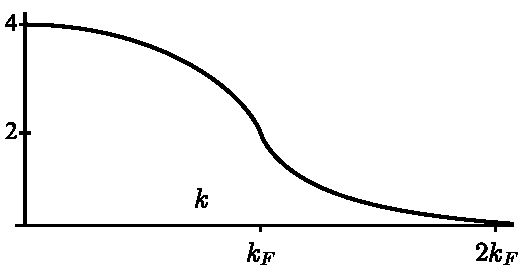
\includegraphics[width=0.72\textwidth]{fig_13.pdf}
\caption*{图 13　$A_k$ 表达式中方括号内的函数随 $k$ 的变化：$k=0$ 处值为 4，$k=k_F$ 处斜率无穷大，横轴标出 $k$、$k_F$、$2k_F$（原书图注仅作 “Figure 13”）}
\end{figure}

由 $A(k)$ 我们可以计算两件事。第一件是平均交换能（exchange energy），它将是 $(1/2N)\sum_k A(k)$。我们看到 $A$ 在 $0.612/r_s$ 的（2 到 4）倍之间变化；平均因子约为 3：$E_{\mathrm{exch}} = -0.916/r_s$，它抵消掉了 $1.2/r_s$ 的 Coulomb 自能中很大的一部分。尽管如此，在 Na 中 $0.25/r_s$ ryd $\cong 0.85$ ev 的差额，已足以移去内聚能的相当大一部分。

剩下的修正是“关联能”，即由于即使是自旋反平行的电子也倾向于彼此保持距离而必须作出的那项修正。关于这一修正项有着浩繁的文献；只需说明这一点：Wigner 以及后来的 Pines (31)，在一类对 $r_s \lesssim 1$ 肯定良好的表达式与另一类对 $r_s \gtrsim 10$ 同样良好的表达式之间，于相当宽的范围内作了内插——尽管对于 $r_s = 4$ 而言，这两类表达式都谈不上有合理的希望能够接近——由此得到如下估计。鉴于它在已知范围内变化不快，而且各种估计彼此相符，我们可以猜测它在 $\pm 20\%$ 的范围内有效：$E_{\mathrm{corr}} = 0.88/(r_s + 7.8)$ ryd。［许多作者所用的并非此式，而是 Wigner 更早的一个表达式；他于 1938 年在一条脚注中对其作了修正 (29)。］用这个表达式我们得到表 4 所给出的结果。

\begin{center}
表 4

\begin{tabular}{lccccc}
\toprule
元素 & 未修正 $E_{\mathrm{coh}}$，ev & $\Delta E_{\mathrm{HF}}$，ev & $\Delta E_{\mathrm{corr}}$，ev & 总计，ev & 实验，ev\\
\midrule
Li & $-2.1$ & $1.19$ & $-1.09$ & $-2.0$ & $-1.65$\\
Na & $-1.15$ & $0.96$ & $-1.02$ & $-1.2$ & $-1.2$\\
Rb & $-0.42$ & $0.73$ & $-0.92$ & $-0.61$ & $-0.85$\\
\bottomrule
\end{tabular}
\end{center}

我必须提醒各位：我在这里给出的这些表并不是权威的，也不代表 Q.D.M. 所已取得的最精确或最好的结果。至于更详细的结果，我请各位去查阅原始文献，特别是 Ham 的文章以及 Brooks 收在 Varenna 夏季学校报告中的文章。正如这后一篇文章所指出的，Ham 所取得的良好符合会因各种进一步的修正而打折扣。能够可靠引出的结论也许只有如下这些：Wigner 对自由电子关联能的估计离正确值并不远；而且我们确实知道碱金属中内聚的真正物理来源。与关联能中 $\pm 0.2$ ev 的误差同量级的修正，可能是费米能中的其他项，而最重要的则是由于波函数并非自由电子波函数而引起的对交换与关联的修正。稍后我们会看到，仅仅在这些效应的公式中塞进一个 $m^*$ 是不合法的，而这些修正的真正本质目前尚不清楚。［不过，可参见不久后将要讨论的 Phillips 的工作 (25)。］这些修正很容易达到关联能的 20\% 的量级。

Q.D.M. 的数值结果中有一个方面引人注目且非常令人鼓舞：在这些金属的压缩率上得到的符合，几乎与在能量上得到的符合同样好。早年的许多计算以及大多数用其他方法所作的计算，给出的压缩率都非常糟糕。毕竟，压缩率是结合能曲线的二阶差分。Q.D.M. 之所以如此之好，其原因可能在于：对所有各项随密度的依赖形式我们确实了解得相当清楚——$E_0$ 项是因为它可以算得非常精确，其余各项则是因为它们由一般性的理论考虑所决定。动能按 $1/r_s^2$ 变化，而交换能、Coulomb 能与关联能则大致按 $1/r_s$ 变化。基于这一想法，用 Bardeen 的半经验状态方程 (27) 常常能够对 pV 曲线得到非常好的拟合：
\begin{equation*}
E = \frac{A}{r_s^3} + \frac{B}{r_s^2} - \frac{C}{r_s}
\end{equation*}

在接着讨论 O.P.W. 方法之前，我现在想先回到交换能上来略作讨论。$A(k)$ 的另一个重要方面是：它代表着对动量为 $k$ 的电子的自能（self-energy）$E_k$ 的一个依赖于 $k$ 的修正：$E_k = \hbar^2 k^2/2m^* - A(k)$。这是诸如交换这类非局域（nonlocal）势的特征行为。对于由各种多体效应所产生的有效势来说，非局域性是常态。这个势是 $A\phi = \int A(\mathbf{r}-\mathbf{r}')\,\phi(\mathbf{r}')\ \mathrm{d}\mathbf{r}'$；由卷积定理，它变换成自能的一个依赖 $k$ 的修正 $A\phi_k = A_k\phi_k$，可以粗略地把它看作一种\emph{有效质量}修正——不过它并非由晶格的周期势所引起，而是由交换空穴随粒子动量的变化所引起。

在采用 Coulomb 相互作用的交换这一特殊情形下，有效质量修正恰好在费米面处发散：由于 $A(k)$ 具有无穷大的负斜率，$\mathrm{d}E_k/\mathrm{d}k\big|_{E_F} = +\infty$ 恰好在费米面处成立。态密度对数式地降到零。假如果真如此，就会与低温比热、自旋顺磁性等方面的许多实验结果相矛盾。Wigner 在原始论文中就已指出：实际上，在真实电子气中，Coulomb 相互作用的长程部分会被近旁其他电子的微小位移所屏蔽（screening），而这些位移同样也牵涉在关联能之中。对这种势屏蔽的一个粗略计算给出有效势 $e^{-k_0 r}/r$，其中 $k_0$ 是 Debye 波数，其量级为 $k_F$。这样一来，$A(k)$ 中的奇性被抹平，有效质量修正不再发散。我们应当强调，“交换空穴”仍然是一个长程的、振荡的函数，在 $k$ 空间的费米面处带有奇性；但它对交换势 $A$ 的影响，则会因相互作用范围的缩短而被抹平。这时 $A(k)$ 对 $k$ 的曲线看上去就像图 14 那样。

\begin{figure}[H]
\centering
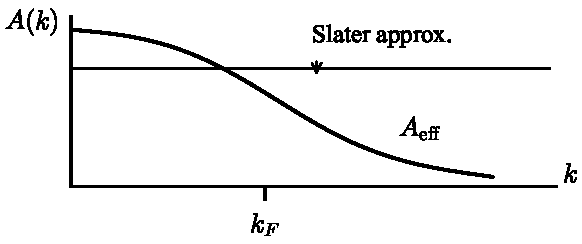
\includegraphics[width=0.72\textwidth]{fig_14.pdf}
\caption*{图 14　交换势 $A(k)$ 与屏蔽后的 $A_{\mathrm{eff}}$ 随 $k$ 的变化，水平线为 Slater 近似，$k_F$ 处的奇性已被抹平（原书图注仅作 “Figure 14”）}
\end{figure}

% ---- B.3 收尾（原书 p.61 / PDF p076 顶部，协调者补译） ----
其净结果是有效质量的减小，在金属密度下其数值可能不大（5\% 到 20\%）。

在实际晶体中，自由电子的密度并不是常数，自由电子模型不再适用，$A$ 也不再是 $A(\mathbf{r}-\mathbf{r}')$ 而是 $A(\mathbf{r},\mathbf{r}')$；它既是非定域的，又是随空间变化的。一个常常采用、源自 Slater (32) 的近似，是在这种情形下忽略 $A$ 的非定域性质，试图把它换成最好的定域势 $A(\mathbf{r})\,\delta(\mathbf{r}-\mathbf{r}')$，后者将正比于局域密度的 $1/3$ 次幂。$\delta$ 函数的傅里叶变换是常数，所以这样做的实质，是用一个适当的平均值代替 $A(\mathbf{k})$（见图~14）。这一近似能够成立的判据是：电子密度相对于交换空穴的尺度变化缓慢，而交换空穴的尺度大致为 $r_s$；此时非定域势所取样的区域将具有大致恒定的交换势。这样的近似在碱金属中是不可想象的——在那里 $r_s > r_{\mathrm{core}}$，因而远大于发生变化的长度尺度——但在 $r_s \sim 1$--$2$ 的多价物质中情形可能要好一些。Phillips 对金刚石（$r_s = 1.3$ (33)）就这一问题作过相当透彻的研究，结果表明 Slater 近似在那里并不严重，尽管对能带结构的某些方面仍有 20\% 到 30\% 的修正，尤其是对从最低态 $k=0$、$L=0$ 量起的费米面整体高度的修正。当然，这正是永远可以预期的一类效应：它对应于真实自由电子气中 $A(\mathbf{k})$ 的动量依赖性。\footnote{关于把核物质当作费米气体的最早评论，大概出自 Van Vleck：他指出在这种情形下，交换对有效质量的修正同样可能导致较轻的 $m^*$——这是一个确实发生并且至关重要的效应。}

\subsection{O.P.W.（正交化平面波）方法}

% 衔接说明：本文件自原书 p.61 的小节标题 “4. The O.P.W. Method” 起译；
% p076 顶部（标题之前）为 B.3 小节的收尾两段及脚注 1（Van Vleck 注），归前一文件负责，此处从略。

% ---- 原书 p.61 (PDF p076) ----
现在我们接着来研究一种方法：它迄今在计算结合能方面从未十分成功过，但在计算能带结构方面却极为成功。这一强有力的方法得以幸运地重新兴起，恰逢多种实验方法已经可以用来细致研究复杂的能带结构——除碱金属外，所有的能带结构都是复杂的——这就使得最近 10 年间人们对固体中电子行为的理解发生了一场彻底的革命。

O.P.W. 方法由 Herring 于 1940 年发明 (34)，Herring 和 Hill (35) 用它计算了 Be 的结合能。所得结合能不太好的这一事实，相当程度上掩盖了如下事实：这一计算很可能给出了非常好的能带结构——正如 Herring 在原始论文中所评论的那样。基本想法如下：基于近自由电子微扰论——亦即以真正的平面波作为初始本征函数——的计算，要想在真实固体中切实可行，希望是微乎其微的。这有两条理由。第一条是：原子芯的势在靠近原子核的区域内实际上变得极其巨大，

% ---- 原书 p.62 (PDF p077) ----
因此根本谈不上把它当作微扰来处理。在某种意义上，我们必须在这个区域内引进一个更加接近精确的解，因为真实的本征函数在那里必定变化迅速，而这种变化只有用 $k$ 矢量非常高的平面波才能描述。

第二条理由更加有说服力。它说的是：即使我们成功地用平面波把这个计算做到无限高阶，其结果多半也不会收敛到对我们的目的而言正确的答案。原因在于：在所有真实金属中都存在若干芯能级（core levels）——在 Be 或 C 中是 $(1s)^2$，在更复杂的原子中还要多得多——相对于我们所关心的价电子能级，它们具有非常大的结合能。于是，在布里渊区内的任何一个 $k$ 处，都存在一个或多个芯带能级，而一个正确计算的最低本征值将趋于这些能级。众所周知，较高本征值的计算是相对困难的事情。

Herring 对这个问题的解法几乎是显而易见的：取作初始波函数的不是平面波，而是对芯能级的波函数正交化了的平面波。只要芯波函数选得相当合理，这至少会解决第二个困难。幸运的是，由于芯能级大多位于来自原子核的强势区——这个势相对来说也已了解得比较清楚——即便是 Hartree 近似对它们也确实相当精确，因为电子-电子相互作用的效应并不十分严重。因此，芯函数的选取并不是一个敏感问题。

Herring 还注意到，选取正交化平面波作为初始函数，至少也部分地解决了第一个问题。在把平滑变化的平面波函数对芯能级正交化的过程中，人们往平面波里引入了在原子核附近聚成尖峰的快速变化。起初人们只是从经验上观察到：这种快速变化似乎恰好能使初始函数成为芯势强区域中波动方程的一个过得去的解，因而这一步骤的收敛速率看来确实快得尚可应付。

现在让我们把理论正式写下来。以某种方式——例如由自由原子的 Hartree-Fock 理论——得到的芯函数，我们记作
\begin{equation*}
\chi_n(\mathbf{r}-\mathbf{R}_j)
\end{equation*}
其中它就是围绕第 $j$ 个原子的第 $n$ 个芯轨道。如果 $\chi$ 确实是一个芯轨道，那么“由 $\mathbf{R}_j$ 到 $\mathbf{R}_j+\mathbf{a}$ 的交叠可以忽略”就必须是一个足够好的近似。（Herring 设计了一些办法，可以对任何残余的交叠作微扰论处理。）于是
\begin{equation*}
\left(\chi_n(\mathbf{r}-\mathbf{R}_j),\ \chi_m(\mathbf{r}-\mathbf{R}_k)\right)=\delta_{nm}\,\delta_{jk}\tag{13}
\end{equation*}
于是，对第一布里渊区内一个给定的 $k$，相应的能带函数恰好就是“紧束缚”函数

% ---- 原书 p.63 (PDF p078) ----
\begin{equation*}
\phi_k^n=\frac{1}{N^{1/2}}\sum_j \exp(i\mathbf{k}\cdot\mathbf{R}_j)\,\chi_n(\mathbf{r}-\mathbf{R}_j)
\end{equation*}
如果式 (13) 得到满足，这些函数同样既正交又归一化。

属于第一布里渊区中给定 $k$ 的各种可能的平面波，可以用倒格子矢量 $K$ 来标记：
\begin{equation*}
\phi_{k,K}(\mathbf{r})=\frac{1}{V^{1/2}}\,e^{i(\mathbf{k}+\mathbf{K})\cdot\mathbf{r}}
\end{equation*}
于是，正交化平面波函数便是
\begin{equation*}
\psi_{k,K}(\mathbf{r})=\phi_{k,K}(\mathbf{r})-\sum_n\left(\phi_{k,K},\ \phi_k^n\right)\phi_k^n(\mathbf{r})\tag{14}
\end{equation*}
其中
\begin{equation*}
\left(\phi_{k,K},\ \phi_k^n\right)=a_{K,n}\tag{15}
\end{equation*}
是平面波与芯函数之间的交叠积分（overlap integral）：
\begin{align*}
a_{K,n}&=\frac{1}{\sqrt{NV}}\int \mathrm{d}\mathbf{r}\ \exp\left[-i(\mathbf{k}+\mathbf{K})\cdot\mathbf{r}\right]\sum_j\ e^{i\mathbf{k}\cdot\mathbf{R}_j}\chi_n(\mathbf{r}-\mathbf{R}_j)\\
&=\frac{1}{\Omega^{1/2}}\int \mathrm{d}\mathbf{r}\ e^{-i(\mathbf{k}+\mathbf{K})\cdot(\mathbf{r}-\mathbf{R}_j)}\chi_n(\mathbf{r}-\mathbf{R}_j)\\
&=\frac{1}{\Omega^{1/2}}\int \mathrm{d}\mathbf{r}\ e^{-i(\mathbf{k}+\mathbf{K})\cdot\mathbf{r}}\chi_n(\mathbf{r})
\end{align*}
这正是 $\chi$ 的波矢为 $(\mathbf{k}+\mathbf{K})$ 的那个 Fourier 分量；或者说，如果你愿意这么看，它是动量空间波函数 $\chi_n(\mathbf{p})$ 在 $\mathbf{p}=\mathbf{k}+\mathbf{K}$ 处的振幅：
\begin{equation*}
a_{K,n}=\chi_n(\mathbf{p}=\mathbf{k}+\mathbf{K})
\end{equation*}
遗憾的是，正交化平面波——即式 (14)——既不归一，彼此之间也不正交。因此我们必须采用处理非正交归一函数的标准做法：

% ---- 原书 p.64 (PDF p079) ----
必须对久期行列式（secular determinant）求解本征值 $E$：
\begin{equation*}
\left|\left(\psi_{k,K},\ (\mathcal{H}-E)\,\psi_{k,K'}\right)\right|=0\tag{16}
\end{equation*}
其中 $E$ 也会出现在某些非对角元之中。式 (16) 的一般元素是可以算出的，只是要付出相当繁重的劳动，它就是
\begin{align*}
E\left(\delta_{KK'}-\sum_n a_{Kn}^{*}\,a_{K'n}\right)&=E_{k+K}^{0}\,\delta_{KK'}\\
&\quad-\left(E_{k+K}^{0}+E_{k+K'}^{0}\right)\sum_n a_{Kn}^{*}\,a_{K'n}+V_{KK'}\\
&\quad-\sum_n\Bigl\{a_{Kn}^{*}\left(\chi_n,\ V\phi_{k,K'}\right)+a_{K'n}\left(\phi_{k,K},\ V\chi_n\right)\Bigr\}\\
&\quad+\sum_n a_{Kn}^{*}\,a_{K'n}\,E_n
\end{align*}
$E_n$ 是第 $n$ 个芯能级。我们已经假定芯带非常窄——交叠为零正蕴含着这一点。$E_k^0$ 是自由电子动能 $\hbar^2k^2/2m$。如你所见，这是一个相当复杂的表达式，不过只要知道了 $V(\mathbf{r})$ 和各芯能级，它的每一项原则上都能直接算出。

当然，实际做法不是求解无限行列式 (16)，而是求解一个有限的行列式，它由审慎地截断所考虑的平面波数目而得到。一般说来，留待求解的久期行列式可能仍然相当大——尽管用现代计算机可以使用相当多的平面波，多达 20 个或更多——但为了容易得到结果并检验收敛性，人们通常把注意力集中在布里渊区的少数几个特殊对称点上。在对称点上，我们可以像前面结合近自由电子模型所讨论的那样，把平面波组成不同对称类型的对称化组合；而周期势的作用不能使不同对称类型相混合。

例如各位当还记得：对 f.c.c. 空间格子、$\mathbf{k}=0$ 的情形，我们可以构成下列几组对称化平面波（symmetrized plane waves），它们全都来自与 $\mathbf{K}=2\pi/a\,(\pm 1,\pm 1,\pm 1)$ 相对应的八个函数的线性组合：

% ---- 原书 p.65 (PDF p080) ----
\begin{align*}
\Gamma_1&:\ \cos\frac{2\pi x}{a}\ \cos\frac{2\pi y}{a}\ \cos\frac{2\pi z}{a} &&\qquad 1\\
\Gamma_2'&:\ \sin\frac{2\pi x}{a}\ \sin\frac{2\pi y}{a}\ \sin\frac{2\pi z}{a} &&\qquad 1\\
\Gamma_{15}&:\ \cos\frac{2\pi x}{a}\ \cos\frac{2\pi y}{a}\ \sin\frac{2\pi z}{a}\ +\ \text{置换} &&\qquad 3\\
\Gamma_{25}'&:\ \cos\frac{2\pi x}{a}\ \sin\frac{2\pi y}{a}\ \sin\frac{2\pi z}{a}\ +\ \text{置换} &&\qquad 3
\end{align*}
在所有这些当中，只有 $\Gamma_1$ 与 $\mathbf{K}=0$ 的平面波 $\phi_0=1$ 相联系。于是，只需求解一个关于 $\Gamma_1$ 的 $2\times 2$ 方程，此外除了对角元的计算以外不需要任何别的方程，我们就已经把九个平面波考虑在内了。我们还可以在此之上再加入 $\mathbf{K}=2\pi/a\,(\pm 2,0,0)$ 等处的六个平面波，办法是把六个对称化平面波
\begin{align*}
\Gamma_{15}&:\ \sin\frac{4\pi x}{a},\ \text{等等} &&\qquad 3\\
\Gamma_1&:\ \cos\frac{4\pi x}{a}\ +\ \cos\frac{4\pi y}{a}\ +\ \cos\frac{4\pi z}{a} &&\qquad 1
\end{align*}
以及一个二维表示 $\Gamma_{12}:\ \cos(4\pi x/a)-\cos(4\pi y/a)$（2）包括进来。这样，我们实际上就把 15 个平面波包括了进来，而所需的久期方程至多是三阶的，并且只有对那三个 $\Gamma_1$ 波才是如此。

遗憾的是，与这一优点相伴的还有一个缺点：在这样的对称点上，正交化过程不仅被简化，而且被过分简化了。在上面的例子中，不妨设想所研究的物质只有 $1s$ 芯电子（这是一个虚构的情形，但足以说明原理）。于是，唯一不会因对称性而自动与芯正交的正交化平面波集合，是对称性为 $\Gamma_1$ 的那些：$\cos(2\pi x/a)\times\cos\times\cos$；$\cos(4\pi x/a)+\cos+\cos$；以及平面波 $\mathbf{k}=0$。这些全都必须对 $1s$ 函数正交化，并把完整的久期行列式解出来——当然，现在它并不十分复杂。在所有其他情形，我们直接只用平面波来做，对其而言久期行列式只不过是
\begin{equation*}
\left|\left(E_{k+K}-E\right)\delta_{KK'}+V_{KK'}\right|=0
\end{equation*}
而且至多是二阶的。

一般说来，在任何一个对称点，总会有某些平面波集合出现这种情形。在 Si 中，需要作 $1s$、$2s$、$2p$ 三种正交化：前两种对着 $\Gamma_1$ 集合，后一种对着 $\Gamma_{15}$。另一方面，$\Gamma_{25}'$ 和 $\Gamma_{12}$ 集合仍然自动地与所有芯正交，因为它们在原子附近具有 d 型对称性；而 $\Gamma_2$ 则好比 $xyz$，是一个 f 型对称性的态：对它来说，直到 Lu 为止都无须作任何正交化。

% ---- 原书 p.66 (PDF p081) ----
这在省去大量麻烦的同时也带来了麻烦，因为这些函数于是保留了十足的平面波特征，在原子芯附近毫无原子型的貌相。为了赋予它们 Bloch 函数所特有的、在芯附近的急速变化，在截断之前必须引入比较多的平面波；O.P.W. 方法对这些函数的收敛相对较慢。不过它并不像人们可能担心的那样慢，因为单从这个例子已经可以看到，我们必须走到相当大的 $K$ 矢量才能找到可与它们组合的波；这背后有一个物理原因，我们很快就会明白。

从一开始，物理上就很清楚：久期方程 (16) 中的各大项之间必定存在大量的相互抵消（cancellation）。矩阵元 $V_{KK'}$ 的性质是：如果没有正交化项，所得能量将会是芯能级非常大的结合能——例如在金刚石中为 $-22.7$ ryd。正交化项以某种方式成功地保证了：没有任何波函数以深于约 $-2$ ryd 的能量被束缚；这个值正是价电子壳层中原子函数的最低能量。因此，在某种意义上，对于被迫与芯能级正交的那些函数，$V(\mathbf{r})$ 这一巨大的吸引性势能除 10\% 之外已全部被抵消掉了。

这种抵消的底层理论——我把它称作“Phillips 消去理论”——Phillips 已勾勒过其轮廓，Cohen 和 Heine (36) 则作了非常漂亮的表述。这里我将沿用后者的讨论。另一篇重要文献是 Austin、Heine 和 Sham (37)。

消去理论的基本想法是：我们要试图找出的波动方程，其满足者不是真实波函数 $\psi_k$——它满足 $[(\mathbf{p}^2/2m)+V(\mathbf{r})]\,\psi_k=E_k\psi_k$——而是 Phillips 所称的 $\psi$ 的“光滑”部分；在本情形中，即平面波部分 $\phi$，正交化项正是要从它里面减去。

那么我们就来做这件事。若严格波函数由式 (14) 给出：
\begin{equation*}
\psi_k=\phi_k-\sum_n\left(\phi_k,\ \phi_k^n\right)\phi_k^n
\end{equation*}
（其中 $E_k^n$ 为芯能级。译注：原书此处印作 $\phi_k^n$，按上下文应为 $E_k^n$。）我们便有
\begin{align*}
\left(\frac{\mathbf{p}^2}{2m}+V\right)\psi_k&=\left(\frac{\mathbf{p}^2}{2m}+V\right)\phi_k\\
&\quad-\sum_n\left(\phi_k,\ \phi_k^n\right)\left(\frac{\mathbf{p}^2}{2m}+V\right)\phi_k^n=E_k\left(\phi_k-\sum_n\left(\phi_k,\ \phi_k^n\right)\cdot\phi_k^n\right)
\end{align*}

% ---- 原书 p.67 (PDF p082) ----
或者，
\begin{equation*}
\left(\frac{\mathbf{p}^2}{2m}+V+V_R\right)\phi_k=E_k\,\phi_k
\end{equation*}
其中
\begin{equation*}
V_R=\sum_n\left(E_k-E_n\right)\ \frac{\phi_k^n}{\phi_k}\ \left(\phi_k,\ \phi_k^n\right)
\end{equation*}
$V_R$ 这样通过用 $\phi_k$ 相除来定义是相当任意的；但当我们看到——但愿如此——$\phi_k$ 在芯区内的变化相对于 $\phi_k^n$ 来说非常小，因而用 $\phi_k$ 相除只不过给出 $\phi_k^n$ 的一个常数倍；而且 $E_k$ 一般比芯结合能 $E_n$ 小，故其变化可以忽略——这时 $V_R$ 便取得了真实的意义。这样一来，$V$ 就有点像一个真正的势了。

它究竟是什么，Cohen 和 Heine 已经讲明白了：它是我们的老朋友——一个非局域势。也就是
\begin{align*}
V_R\phi_k(\mathbf{r})&=\int \mathrm{d}\mathbf{r}'\ V_R(\mathbf{r},\mathbf{r}')\,\phi_k(\mathbf{r}')\\
V_R(\mathbf{r},\mathbf{r}')&=\sum_n\left(E_k-E_n\right)\phi_k^n(\mathbf{r})\left(\phi_k^n(\mathbf{r}')\right)^*
\end{align*}
这一点通过积分立即可见。Phillips 的论断——实质上就是上面的物理推理——是：$V_R$ 是一个排斥势（因为 $E_n$ 为负），它常常几乎把 $V$ 完全抵消掉。

Cohen 和 Heine 用下面的办法在数学上证明了这个抵消：考察方程 (14)——它实质上是以严格波函数 $\psi_k$ 来定义“光滑”波函数 $\phi_k$ 的——我们看到，这个定义绝非唯一。毕竟，在我们所考虑的应用中，平面波集合 $\phi_{k+K}$ 是一个完备集（complete set），因此即便是函数 $\phi_k^n$ 也可以用它们来展开。于是，如果我们愿意，实际上可以不用正交化、完全用平面波集合写出 $\psi_k$，但这当然会给出一个收敛性极差的平面波展开；或者，原则上我们也可以把正交化项以任意选定的比例分配在 $\phi$ 与显式项之间。

% ---- 原书 p.68 (PDF p083) ----
这意味着，我们必须凭某个附加的明确条件来规定所谓“光滑波函数 $\phi$”的含义。实际上我们清楚它指的是什么：它就是我们所能侥幸得到的最接近于少数几个平面波的那个东西。Cohen 和 Heine 指出，表达这一想法的一个数学方式，是要求有效势 $(V+V_R)$ 尽可能地弱：
\begin{equation*}
\left(\phi,\ (V+V_R)\,\phi\right)/\left(\phi,\phi\right)=\text{minimum}
\end{equation*}
由这一条件出发，经直接的数学演算，可以得到 $(V+V_R)\phi$ 所满足的如下方程：
\begin{align*}
(V+V_R)\phi&=V\phi-\sum_n\left(\phi_k^n,\ V\phi\right)\phi_k^n\\
&\quad+\left(\phi,\ \left[V+V_R\right]\phi\right)\sum_n\left(\phi_k^n,\ \phi\right)\phi_k^n
\end{align*}
于是这一有效势的对角元就是
\begin{equation*}
\left(\phi,\ \left[V+V_R\right]\phi\right)=\frac{\left(\phi,\ V\phi\right)-\sum_n\left(\phi,\phi_k^n\right)\left(\phi_k^n,\ V\phi\right)}{1-\sum_n\left|\left(\phi_k^n,\ \phi\right)\right|^2}
\end{equation*}
相应的非局域势就是
\begin{equation*}
(V+V_R)(\mathbf{r},\mathbf{r}')=V(\mathbf{r})\left\{\frac{\delta(\mathbf{r}-\mathbf{r}')-\sum_n\phi_k^{*n}(\mathbf{r})\,\phi_k^n(\mathbf{r}')}{1-\sum_n\left|\left(\phi,\ \phi_k^n\right)\right|^2}\right\}\tag{17}
\end{equation*}
（注：Austin、Heine 和 Sham (37) 后来已经证明，这个分母是不必要的。）

这样我们就证明了两件事：我们所使用的有效势在上述意义下是可能的最弱者；而且它可以写成式 (17) 的形式。现在请注意
\begin{equation*}
\sum_{\text{all states}}\phi_k^{*n}(\mathbf{r})\,\phi_k^n(\mathbf{r}')=\delta(\mathbf{r}-\mathbf{r}')\tag{18}
\end{equation*}

% ---- 原书 p.69 (PDF p084) ----
因此，除了分母中的归一化因子之外，\emph{这个势已被束缚态的一个线性组合抵消到了它所能达到的最有效程度}。换一种说法：抵消的程度正比于束缚态在 $V$ 很大的区域内构成完备集的程度。Cohen 和 Heine 为 Si 给出了一幅令人赞叹的图，显示这种抵消可以达到何等好的程度。（图 15）（把图画成一个局域势时，是利用了如下事实：对 $s$ 态来说，就与芯函数作积分的目的而言，$\phi$ 是一个常数，因而\emph{对给定的 $l$}，非局域性无关紧要。）

\begin{figure}[H]
\centering
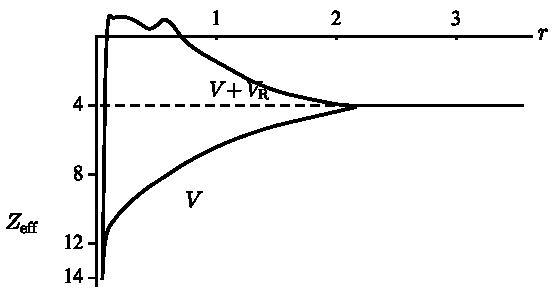
\includegraphics[width=0.72\textwidth]{fig_15.pdf}
\caption*{图 15　Si 中势的抵消：$V$ 与 $V+V_R$ 的有效电荷 $Z_{\mathrm{eff}}$ 随 $r$ 的变化（纵轴刻度自上而下为 4、8、12、14），$V$ 在芯区内深达 14，$V+V_R$ 很快趋于虚线所示的约 4 的浅势；横轴 $r$ 标 1、2、3（原书图注仅作 “Figure 15”）}
\end{figure}

典型地说，归一化因子 $1\big/\left(1-\sum_n\left|\left(\phi,\ \phi_k^n\right)\right|^2\right)$ 相当接近于 1：大约在 1.1 左右（见上面的注）。

注意，势的非局域性对于使势对不同 $l$ 值表现得颇为不同这一点至关重要。例如，正如我们已经指出过的，当芯能级中没有 p 型的能级时，p 能级就不存在抵消；我们可以由观察到此时
\begin{equation*}
\int \mathrm{d}\mathbf{r}'\ V_R(\mathbf{r}-\mathbf{r}')\,\phi_p(\mathbf{r}')=0
\end{equation*}
看出这一点，因为它等同于
\begin{equation*}
\int \mathrm{d}\mathbf{r}'\ V(\mathbf{r})\,\phi_{1s}(\mathbf{r})\,\phi_{1s}(\mathbf{r}')\,\phi_p(\mathbf{r}')
\end{equation*}
这里的 $\phi_p$ 是指某个必然具有 p 对称性的对称化平面波，例如一个 $\Gamma_{15}$ 组合。一般说来，这种抵消就不那么完全——$l$ 值越高，就越是如此。对此有一个非常明显的原因：只要考察角动量为 $L$ 的轨道的径向波动方程

% 衔接说明：末句在原书 p.69 末行中断（p.85 起首为 “complete for higher and higher l values.”），由下一文件续译。

% 衔接说明：本文件为小节 “O.P.W.（正交化平面波）方法” 的后半，不含小节标题。
% 首行承接原书 p.69（PDF p084）末句 “In general, the cancellation is less”，
% 本文件自 “complete for higher and higher l values.” 起续译（与 ch2_B4a.tex 末行拼接）。

% ---- 原书 p.70 (PDF p085) ----
对此有一个非常明显的原因：只要考察角动量为 $L$ 的轨道的径向波动方程
\begin{equation*}
\frac{\mathrm{d}^2 u_L}{\mathrm{d}r^2} - \left[\frac{L(L+1)}{r^2} + V(r)\right] u_L(r) = E_L u_L(r)
\end{equation*}
并勾画出其中的势能项（图 16）。我们看到，离心势项把束缚态从 $V$ 的内部区域排除出去，因此对较大的 $L$，束缚态无论如何也不可能为正是 $V$ 最强的那个区域本身构成一个完备集。尽管如此，虽然这个想法并没有明显地出现在数学表述之中，

\begin{figure}[H]
\centering
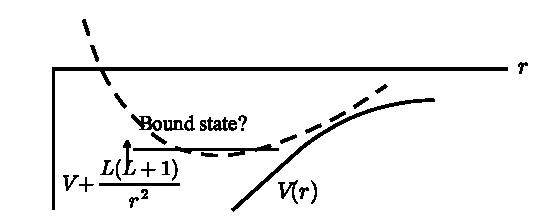
\includegraphics[width=0.72\textwidth]{fig_16.pdf}
\caption*{图 16　径向方程中势能项的草图：实线为 $V(r)$，虚线为离心势 $V + \frac{L(L+1)}{r^2}$，其谷底处标有 “Bound state?”（束缚态？）（原书图注仅作 “Figure 16”）}
\end{figure}

$V$ 的大矩阵元对这些较高的 $L$ 态实际上起不了多大作用，因为平面波态同样不能很有效地穿入芯区——离心项对它们同样起作用。这样看来，必然要发生的抵消之中，有一部分来自 $k$ 相当高的平面波，这也是这些态收敛性差的部分原因。事实上，Heine 曾指出，一定程度的抵消会显式地出现在久期方程之中。

我相信，这里的抵消理论仍然有进一步改进的余地。读者当中做核物理的人也许已经注意到，其中某些想法——无论是在 Q.D.M. 中还是在“被抵消的 O.P.W.”（cancelled O.P.W.）中——与多重散射理论（multiple scattering theory）和有效力程理论（effective range theory）的技术、以及在该理论中把散射矩阵 “T” 用作有效势的做法（38），有着惊人的相似。我想，通过与多重散射理论作类比，大概还能做成更多的事情，特别是把高动量的连续谱态连同束缚态一起从问题中消去。\footnote{在写完这些讲稿之后我获悉，Ham 与 Segall 的 Green 函数方法［Phys. Rev., \textbf{124}, 1786 (1961)］正是朝这个方向迈出的第一步：这一方法以及增广平面波方法（augmented plane-wave method）（M. M. Saffren，学位论文，M.I.T.，1959）之所以收敛极佳，很可能正是由于它们与多重散射理论的相似性。（译注：原文此处印作 “N.I.T.”，应为 M.I.T.。）}

% ---- 原书 p.71 (PDF p086) ----
用带抵消的 O.P.W. 所完成的详细定量工作是专家的课题。另一方面，我倒想提请各位注意它有助于说明的固体行为的若干定性特征。这些特征基本上有两类：（1）“好金属”行为中由它解释的那些方面；（2）固体量子化学中由 O.P.W. 何时良好、何时失效来解释的那些方面。

1. 这些方面中对剑桥的人士来说更熟悉的一个，是近自由电子图像在定性解释所观测到的纯金属费米面方面的显著成功。我想这方面已广为人知，无须进一步讨论。在这一推广的几个显著的失败之中，铜是一例：其中相关的芯能级——d 能级——下得不够深，无法用正交化来处理；而各价半导体（valence semiconductors）定量地看，离开自由电子球其实并不那么远。

第二个特征，是所谓“刚性能带”（rigid band）模型在无规合金和液态金属中的经验成功——正如 Heine 与 Ziman (39) 所强调的，这一成功实在可观。在这个模型中，人们忽略物质的无规背景结构，假装其行为受某种平均能带的控制，这个能带含有各组分所贡献的价电子的平均数目。在模型的极端形式下，人们假定金属的性质只由每原子的价电子数目决定，而不管这些电子由哪些原子贡献。在某些情形下，甚至晶体结构也能靠这种“对周期表取平均”的办法来预言。一个引人注目的例子是 Mo 与 Ru 的合金：它在晶体结构和其他若干性质上都模拟人造元素锝，而在所有这些性质上 Mo 和 Ru 都与 Tc 大相径庭 (40)。近来发现，越来越多的性质随电子/原子比这个参量相当平滑地变化，而这个参量当然只是决定相应费米面的大小 (10)。我不想造成一种错误印象，似乎刚性能带总能对合金与化合物的所有性质给出正确的描述——也许它们不奏效的时候比奏效的时候更多，特别是在混合彼此差别很大的金属时——而是想说：鉴于决定金属大部分物理性质的，是各种效应之间敏感的平衡，它们居然能够奏效，这件事本身就相当令人惊讶。

2. Phillips、Cohen 与 Heine 强调了抵消定理与实测出现的价晶体（valence crystals，有别于金属）之间的关系。在周期表中 $Z$ 较低的成员里，可以用来展开式 (18) 中 $\delta$ 函数的芯轨道少得多。这意味着，即便在较低的元素中，势的 $s$ 部分的抵消效率也较低；而在第一行中根本没有 p 抵消，d 抵消则要到第二长周期的末尾——从镓开始——才出现。于是，剩下的有效势 $(V + V_R)$ 将是周期表行数的减函数——例如从 C 到 Si 到 Ge 到 Sn 到 Pb 依次减小。因此，较早的成员将有更强的区界、更宽的禁带，以及形成开放价结构的更大的能量上的好处。所有这些预言都在第四列的这些元素中得到漂亮的例证。

至于随周期表第二个维度（即沿一行）的变化，则讨论得没有那么透彻。我想这是一个同样能被 O.P.W. 思想照亮的课题，我愿在此稍作讨论。

% ---- 原书 p.72 (PDF p087) ----
下面的讨论将基于这样一个事实：判定固体中价电子的波函数能否被相当好地描述为一组微扰效应相对较小的正交化平面波，实际上有两条判据。第一条我们已经见过——即芯能级必须相当深，使得正交化所给出的有效势的内芯部分已被相当好地抵消，而且芯能级不会强烈地混入价能级之中。

第二条判据可以这样来理解：从能量上看，固体中原子的电子组态要想与自由原子的相差悬殊，是完全不可能的。这一点当然已被实验充分证实：固体中原子的 X 射线结构因子与自由原子相比，从不曾有过挪动一两个以上电子那样严重的差异。各位当中也许有人注意过关于 X 射线测量的那场讨论：测量似乎表明铁在固体中少了四个 d 电子；虽然这些实验后来当然被证明是错的，但这件事至少促成了 Herring 的决定性论证 (41)：挪动这四个电子所需的能量，根本不可能来自内聚中所涉及的那几类能量。把两三个电子挪动一个与 Bohr 半径 $a_0$ 相比可观的数量——从一个壳层挪到另一个壳层——要付出若干 Rydberg 的能量。

因此，第二条重要判据是：\emph{我们预期价电子具有的那个原子波函数，必须能够相当好地用 O.P.W. 费米海内平面波态的占据来描述。}

碰巧，在某些条件下，原子态的构造确实不坏，足以按那种方式被近似。为说明这一点，我们可以去查原子波函数的 Fourier 变换，即它们在动量空间中的波函数［例如查 Bethe-Salpeter 的书，文献 (42)］。举几个例子：$1s$ 函数为
\begin{equation*}
\phi_{1s} = A\,\mathrm{e}^{-\kappa r}
\end{equation*}
而它的（未归一化的）Fourier 变换是
\begin{equation*}
\frac{\kappa}{\left(\kappa^2 + k^2\right)^2}
\end{equation*}
$2p$ 函数的则是
\begin{equation*}
\frac{\kappa^2 k\,Y_{1m}(k)}{\left(\kappa^2 + k^2\right)^3}
\end{equation*}
$3d$ 函数的则是

% ---- 原书 p.73 (PDF p088) ----
\begin{equation*}
\frac{\kappa^3 k^2}{\left(\kappa^2 + k^2\right)^4}\,Y_{2m}
\end{equation*}

这些函数的草图见图 17。当 $k$ 增大时，所有这些函数都在 $k = \kappa$ 附近相当陡峭地下降。如果费米面离这一点不太远，用 O.P.W. 便可对原子函数得到一个不错的近似。

\begin{figure}[H]
\centering
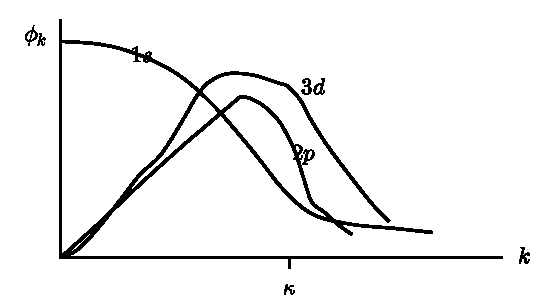
\includegraphics[width=0.72\textwidth]{fig_17.pdf}
\caption*{图 17　动量空间波函数 $\phi_k$ 随 $k$ 的变化：$1s$、$3d$、$2p$ 三条曲线均在 $k \approx \kappa$ 附近陡降（原书图注仅作 “Figure 17”）}
\end{figure}

如果考虑一个由原子函数 $\phi_{nl}$ 组成的 Bloch 波，便容易形象化地看出作出这种近似的第二条判据。对这样一个波，一个合理的近似可以是
\begin{equation*}
b_{\mathbf{k};nl} = \mathrm{e}^{i\mathbf{k}\cdot\mathbf{r}}\sum_j \phi_{nl}(\mathbf{r} - \mathbf{R}_j)
\end{equation*}
立即可见，这样一个函数的动量空间表示是
% 校注：原书求和号下印作小写 k；按物理意义（下页“与 k 由一个倒格矢相连的
% 每一个点”）求和指标应为倒格矢 K，此处按本意转写。
\begin{equation*}
b_{\mathbf{k};nl}(\mathbf{p}) = \sum_{\mathbf{K}} \delta_{\mathbf{p},\,\mathbf{k}+\mathbf{K}}\,\phi_{nl}(\mathbf{k} + \mathbf{K})
\end{equation*}

% ---- 原书 p.74 (PDF p089) ----
在与 $\mathbf{k}$ 由一个倒格矢相连的每一个点上，它取值 $\phi_{nl}(\mathbf{k} + \mathbf{K})$。以 $1s$ 函数为例在一维情形下把这一点形象化，我们可以把这个函数画成图 18 那样。在动量空间中，我们在 $\mathbf{k} + \mathbf{K}$ 的每个值处都有一个尖峰，其高度由原子动量空间波函数在该点处的大小给出。

\begin{figure}[H]
\centering
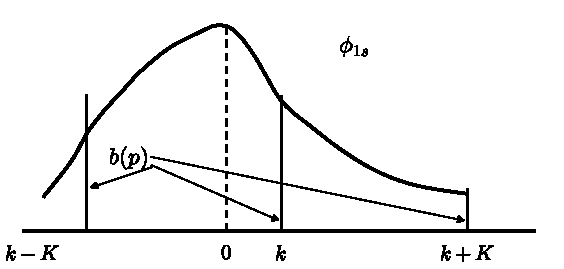
\includegraphics[width=0.72\textwidth]{fig_18.pdf}
\caption*{图 18　一维动量空间中的 $b(p)$：在由倒格矢与 $k$ 相连的各点 $k-K$、$0$、$k$、$k+K$ 处的尖峰，其高度由原子动量空间波函数 $\phi_{1s}$（钟形曲线）在该点的大小给出（原书图注仅作 “Figure 18”）}
\end{figure}

近自由电子模型中的波函数由单个平面波构成，充其量由少数几个能量十分接近的平面波构成。于是，比方说像上图中那样，如果 $\mathbf{k}$ 与 $\mathbf{k} - \mathbf{K}$ 都带有大的尖峰，而能量又不十分相近，这两类波函数就会非常不同。也就是说，$\mathbf{K}$ 矢量相对于 $k_F$ 不得太小，而 $k_F$ 必须 $\approx \kappa$。这等价于说：重要的布里渊区边界不得深入费米面之内太远，因为布里渊区边界恰恰就是 $|\mathbf{k} - \mathbf{K}|$ 等于 $|\mathbf{k}|$ 的地方，而远在 BZ 边界之外，$|\mathbf{k}|$ 便比 $|\mathbf{k} - \mathbf{K}|$ 大出相当多。毫无疑问，这一要求容许相当大的宽容度，但可以肯定，当
\begin{equation*}
|\mathbf{k} - \mathbf{K}| < \frac{3}{4}\,|\mathbf{k}|
\end{equation*}
左右时，这两类函数之间就不再有多少相似之处了。

这一要求的物理意义无非是：近自由电子图像无法很准确地描写变化剧烈的电子密度，因此，如果波函数的线度 $(1/\kappa)$ 比原子间距 $(1/K)$ 小，O.P.W. 就不可能是好的近似。换一个角度看：当 $1/\kappa$ 太小时，剩余的芯势开始变得太强。头一个要求在物理上同样不难理解：原子波函数中的动量分布与固体中的动量分布必须在大致相同的最大动能处截止；这就要求 $\kappa \approx k_F$。

% ---- 原书 p.75 (PDF p090) ----
这些要求中的头一条给了我们一个关于“好金属”行为的非常直截了当的判据；我们已经看到，波函数中的截止点与 $k_F$ 必须落在彼此非常靠近的地方，因而 BZ 不得深入费米球之内太远。但至少在 Bravais 的简单晶格中我们知道，第一布里渊区恰好含有每原子两个电子态，于是，若价电子数为 $Z$，则
\begin{equation*}
\text{BZ 的平均半径} = k_F \Big/ \left(\frac{Z}{2}\right)^{1/3}
\end{equation*}
（当 $Z = 2$ 时，BZ 的体积 = 费米球的体积。）因此这非常直接地就是对 $Z$ 本身的一个限制：它表明，$Z$ 大到 4 或 5 时还可以得到合理的拟合，但从此往后波函数将开始在径向方向上变化得非常快，平面波模型便行不通了。

看一看这些想法沿周期表的两个典型的行如何展开是很有教益的：一个是第二短周期，Na、Mg 等；另一个是第一过渡系，K、Ca、Si、Ti、……（译注：原文如此，此处 “Si” 应为 “Sc”。）

在 Na 等所在的一行中，我们先填充 $3s$ 能级，然后再填充 $3p$ 能级。$3s$ 与 $3p$ 原子能级在其动量空间表示中，正如在其径向空间函数中一样，带有径向节点（radial nodes）；但正交化过程将使恰好相应的节点结构出现在 O.P.W. 函数之中。因此，我们可以在一个“抹平”的空间中进行思考——其中径向节点被忽略——并假定波函数在这个“抹平”空间中的形状恰恰就是 $1s$ 或 $2p$ 函数的形状。

% 校注：原书此处指数印作 $r^{l'}$（l 后带一撇状墨点），按 Slater 波函数本意
% 转写为 $r^{\,l}$。
1930 年，Slater 从若干 Hartree 计算和各种经验数据出发加以推广，得出了一个非常成功的近似原子波函数与“屏蔽常数”（screening constants）(43) 的体系，供原子和分子计算使用。这些是抹平了的无节点函数，形式为 $r^{\,l}\,\mathrm{e}^{-\kappa r}$；而且看来，在我们的计算中所应使用的 $\kappa$ 多半恰好就是这些公式中的 $\kappa$。这些屏蔽常数和波函数，常被用作原子重要外区中的势以及相应波函数的一个相当粗糙的估计。我们在这里对这些元素给出：由金属中的原子体积算出的 $k_F$、由 Slater 按上述办法算出的 $\kappa$，以及 $\kappa_{1/2}$ 这个量——即原子动量函数降至其峰值约一半时的那个 $k$。见表 5。符合得并不完美（注意 Mg 和

\begin{table}[htbp]
\centering
{\bfseries 表~5}\\[5pt]
\begin{tabular}{lccccc}
\toprule
 & Na & Mg & Al & Si & P\\
\midrule
$\kappa$ & $1.39\times10^{8}$ & $1.80$ & $2.20$ & $2.60$ & $3.00$\\
$\kappa_{1/2}$ & $0.87$ & $1.12$ (p:1.6) & $2.00$ (s:1.4) & $2.32$ & \\
$k_F$ & $0.90$ & $1.36$ & $1.55$ & $1.84$ & \\
\bottomrule
\end{tabular}
\end{table}

% ---- 原书 p.76 (PDF p091) ----
\noindent Al 中的误差表明，在这两种情形下 s 与 p 的性质有所混合），但它一点也不坏；而且令人感到有趣的是：仅仅看一看原子波函数的形状，就能把固体的体积估计得多么漂亮。P 有各种各样复杂的晶体结构，一点也不像金属，也不遵守 $\kappa_{1/2} \cong k_F$ 的关系。因此，P、S 和 Cl 无法纳入 O.P.W. 理论：因为要使价电子分布相当均匀，所需的密度会高到使费米能从而平均动能远高于原子中的相应数值。换一种说法：在原子中，壳层简并（shell degeneracy）的存在使得一个填充得相当稠密的电子壳层可以在不付出过多动能的情况下被填满，因为不相容原理是凭借不同动量分量之间相当复杂的相位关系而得到满足的。这一效应只在壳层中电子数多于两三个的那些元素中才重要；但在这些元素中，它阻碍了真金属的形成，因为在真金属中这些相位关系必然要被破坏，而在芯附近维持给定电子密度所需的动能也就会太高。

在 P、S、Cl 中，正如在 N、O、F 中一样，其结果是形成共价键合的分子体系，其中 p 壳层的空穴在很大程度上仍保持其原子 p 函数的身份，并形成有方向的、饱和的共价键。

同样的过程也发生在过渡系中，只是结果不同。这里，所涉及的电子被正交化于 $(1s)^2$、$(2s)^2$、$(3s)^2$、$(2p)^6$ 和 $(3p)^6$。于是，单凭正交化本身，它们便可以带上 $4s$、$4p$ 和 $3d$ 的性质。$k$ 接近零的 O.P.W. 不可能带有可观的 d 性质，只能带有弱的 p 性质；因此，自然而然，起初在 K 中甚至在 Ca 中，O.P.W. 实际上就是 $4s$ 波函数。然而，在较高的 $k$ 值处，$3d$ 函数与 $4p$ 函数之间开始出现竞争。$4s$ 函数对 $4p$ 有有效的屏蔽，对 $3d$ 则没有；而较高的 $n$ 值意味着 $\kappa_{4p} < \kappa_{3d}$，于是在这一点上，$4p$ 函数在 $k$ 空间中的密度可以忽略，而电子——本质上仍是 O.P.W.——开始填充 $3d$ 能级。把屏蔽常数 $\kappa$ 与相应的费米动量加以比较即可表明这一点，见表 6。实际上，这里的符合甚至比前面还要好；而且显然，Sc、Ti 甚至 V 都是相当令人满意的 “O.P.W. 金属”。（括号中的数值是在如下假定下算出的：在这一系列的中段附近，
\begin{table}[htbp]
\centering
{\bfseries 表~6}\\[5pt]
\begin{tabular}{lccccccc}
\toprule
 & K & Ca & Sc & Ti & V & Cr & Mn\\
\midrule
$\kappa$ & $1.1\times10^{8}$ & $1.4$ & $1.65$ & $2.05$ & $2.45$ & $2.85$ & $3.25$ ($\kappa_{3d}$)\\
$\kappa_{1/2}$ & $0.68$ & $0.87$ & $1.65$ & $2.05$ & $2.45$ & $2.85$ & $3.25$ ($\kappa_{3d}$)\\
 & & & & & $(2.2)$ & $(2.65)$ & $(3.22)$\\
$k_F$ & $0.75$ & $1.12$ & $1.59$ & $1.89$ & $2.19$ & $2.47$ & $2.57$\\
\bottomrule
\end{tabular}
\end{table}
% 上句未完，接原书 p.77（PDF p092，不属本文件范围）。
4s 将开始再度变空。）然而在 Cr 和 Mn，以及在某种程度上在 V 中，晶格开始变得远比 3d 电子的 $\kappa$ 所要求的稀疏，于是“3d 带”作为一个实体——有别于那些恰好在核附近才带有 3d 性质的单纯 O.P.W.——开始成形。

然而，由于未填满的 4s-4p 壳层的存在，这里的行为与 p 壳层系列中的行为颇为不同。4s-4p 壳层总保持着一定的占据，随着越来越多的 d 能级被占据、原子彼此相距相对更远，“O.P.W.”费米面便失去 3d 电子，回到只适合 4s-4p 电子的情形。于是在 V 与 Mn 之间的某处，d 带本身——作为由处于近似原子状态的电子构成的紧束缚带——得以成形；在此点之前，d 带与其他任何能带在定性上并无区别。

“内层”能带在这一点上的出现，以行为的巨大变化为标志，正如 O.P.W. 在 p 壳层的失效以分子结构与价结构的出现为标志一样。这里金属性得以保留，但内层电子的特征磁性开始显露——表现为 3d 行中实际的铁磁性与反铁磁性，以及 Pd 族和 Pt 族中的高磁化率与非典型行为。

在这一段题外话中，我试图说明：近满壳层中的空穴与近空壳层中的电子，为什么以及如何在其量子化学性质上表现得截然不同；也试图说明近自由电子图像在哪里、又为什么不能再指望奏效。我相信这样的分析以前从未有人做过。

\section{有微扰场存在时的单电子能带理论}

\subsection{引言}

在离开单电子理论这一主题之前，讨论当通常的周期场上叠加某种非周期微扰时固体中电子的行为，似乎是相当重要的。自然，对固体中处于完全平衡的自由电子所做的实验，无法告诉我们多少关于它们的信息——充其量，除总能量之外，我们至多能通过比热，或者（若运气好的话）通过 X 射线与光学光谱的测量，了解到态密度。为了研究能带结构，我们必须先微扰它。微扰可以由外加的电场和/或磁场构成——相对于原子尺度而言，它们实际上可视为恒定——也可以由周期势受到这种或那种扰动而产生的局域微扰势构成——杂质、位错（dislocation）、表面等等。

自然，真正微弱而局域的微扰——例如由与核磁矩的超精细相互作用、或由两种同位素核之间的差异所引起的微扰——可以用寻常的微扰论处理而无明显的复杂性。真正强的局域微扰——通常由结构中的间隙原子或缺失原子（空位）所引起——则无论在固体中还是在别处，都是一个本质上困难的问题。

% ---- 原书 p.78 (PDF p093) ----

另一方面，碰巧固体中人们感兴趣的最常见一类微扰，是这样一类：它们在总体上可以很强，却相对于原子尺度缓变。例如，均匀电场在哈密顿量中给出一个微扰项 $eEx$（译注：原书排印作 $Eex$），即使 $E$ 很小，它在大晶体中也能变得要多大有多大：$x \to \infty$。均匀磁场在数值上同样可以很大：矢量势可取为 $\mathbf{r} \times \mathbf{H}/2$，它随位置矢量 $\mathbf{r}$ 线性增长。由位错、带电杂质、激子（exciton）、表面等等引起的势分布，也常常是缓变而幅度很大的。正是在这个极限下，“有效哈密顿量”（effective Hamiltonian）理论可以指望是有效的。

在这个理论中，所作的假定是：电子完全在单独一支能带的状态之间运动。这一假定的正当性我们稍后再讨论，但它显然足够合理：一个近乎恒定而平滑变化的势，可以使电子在能量几乎相同的状态之间绝热地来回移动，却不会引起向其他能带的真实跃迁。

我将首先在“有效哈密顿量”或“有效质量”（effective mass）近似下、并在上述假定之内，对电子的动力学作一简短讨论；然后再较深入地考察这一近似的某些背景。有不少文献对其中电子动力学有相当完整的讨论：Ziman (3) 论电场与磁场，Kohn 在《Seitzschrift》第 5 卷中论杂质态（impurity states）(44)，Wannier（文献 4 第 6 章）——我将多少遵循其进路——以及其他多种。Kittel 对“有效质量”的缘由有一段相当漂亮的定性讨论，我推荐作为配套读物（第 2 版，第 288 页），因为我这里不打算采用那种讲法。Wannier 的书在背景论证方面相当不错，不逊于任何参考文献，只有一部例外——它艰深然而完备：即《Seitzschrift》第 13 卷中的 E. I. Blount。

这个问题在如此长的时间里始终是一个活跃课题，本身就值得注意。相应的自由电子结果早在 1930 年就已知道——即 Landau 的抗磁性——其后不久，Jones 和 Zener 以及 Peierls 分别就电场情形和磁场情形，把它们推广到有效哈密顿量近似下的“准自由”电子 (46)。尽管如此，第一次试图体面地推导这些结果、并理解它们在何种意义上是近似的，来自 Wannier 1937 年关于 Wannier 函数的开创性论文。Seitz 书中的推导相当不完整。同样，这一近似的第一次失效由 Zener 于 1934 年——即 Zener 效应——以及 Houston 于 1940 年讨论过。然而，只有靠过去十年间 Luttinger、Adams、Wannier、Kohn、Blount 和 Gibson 的工作，人们才感到对这一问题达到了大概是最终的理解 (45)。有点令人惊讶的是，求解一个形式特别简单的单粒子 Schrödinger 方程竟然需要这一番功夫；而这些结果恰恰生动地表明，即便是自然界最简单的现象，其细节也可以何等复杂。

那么让我们假定：在缓变势存在时，电子确实保持在单独一支能带之内，其能量曲线为 $E_n(\mathbf{k})$——我们讨论的是第 $n$ 支带。

% ---- 原书 p.79 (PDF p094) ----

马上就引进 Wannier 函数（Wannier functions）$a_n(\mathbf{r} - \mathbf{R}_j)$ 的概念是很有教益的。这些函数由一个能带的 Bloch 函数
\begin{equation*}
b_n(\mathbf{k},\mathbf{r}) = \mathrm{e}^{i\mathbf{k}\cdot\mathbf{r}}\, u^n_{\mathbf{k}}(\mathbf{r})
\end{equation*}
出发，通过如下的 Fourier 分析得到：
\begin{equation*}
a_n(\mathbf{r} - \mathbf{R}_j) = N^{-1/2} \sum_{\mathbf{k}} \mathrm{e}^{-i\mathbf{k}\cdot\mathbf{R}_j}\, b_n(\mathbf{k},\mathbf{r}) \tag{19}
\end{equation*}
于是
\begin{equation*}
b_n = N^{-1/2} \sum_{\mathbf{R}_j} \mathrm{e}^{i\mathbf{k}\cdot\mathbf{R}_j}\, a_n(\mathbf{R}_j)
\end{equation*}

在紧束缚带中，$a_n$ 显然就是原来的紧束缚函数，因为此时 $u^n_{\mathbf{k}}(\mathbf{r})$ 与 $\mathbf{k}$ 无关，而且 $\sum_{\mathbf{k}} \to \delta(\mathbf{r} - \mathbf{R}_j)$；否则，$a_n$ 是一组适当正交且归一的函数，多少局域在格点 $\mathbf{R}_j$ 附近。在单带理论中，$a_n(\mathbf{r} - \mathbf{R}_j)$ 代表所能达到的最接近位置本征函数的东西；对自由电子，它们对应于 $\delta(\mathbf{r} - \mathbf{R})$。让我们定义一个算符 $\mathbf{R}$，使得 $\mathbf{R}\, a_n(\mathbf{r} - \mathbf{R}_j) = \mathbf{R}_j\, a_n(\mathbf{r} - \mathbf{R}_j)$。在 $\mathbf{k}$ 只占据第一区、而 $\mathbf{R}$ 以一组分立的格点位置为本征值这两个限制之下，它们代表一对彼此共轭的变量，类似于自由电子理论中的 $\mathbf{p}$ 和 $\mathbf{r}$，即
% 校注：按本页下文的推导（$i\,\partial/\partial\mathbf{R}$ 等价于 $\mathbf{k}$），
% 此对易子似应为 $[\mathbf{k},\mathbf{R}] = i$；原书印作 “= 1”，照录。
\begin{equation*}
[\mathbf{k}, \mathbf{R}] = 1
\end{equation*}
这是因为——按定义——
\begin{align*}
i\,\frac{\partial}{\partial\mathbf{R}}\; a_n(\mathbf{r} - \mathbf{R}_j) &= i\,\frac{\partial}{\partial\mathbf{R}_j}\; a_n(\mathbf{r} - \mathbf{R}_j) \\
&= \sum_{\mathbf{k}} \mathbf{k}\, b_n(\mathbf{k},\mathbf{r})\, \mathrm{e}^{i\mathbf{k}\cdot\mathbf{R}_j}
\end{align*}
［把 (19) 代入 $a_n$］。于是 $i(\partial/\partial\mathbf{R})$ 等价于 $\mathbf{k}$，反之亦然。现在，若 $V(\mathbf{r})$ 缓变，我们可以近似
\begin{equation*}
V(\mathbf{r})\, a_n(\mathbf{r} - \mathbf{R}_j) \simeq V(\mathbf{R}_j)\, a_n(\mathbf{r} - \mathbf{R}_j) = V(\mathbf{R})\, a_n(\mathbf{r} - \mathbf{R}_j)
\end{equation*}

% ---- 原书 p.80 (PDF p095) ----

一般说来，对于缓变的磁微扰或电微扰，可以有效地假定 $V(\mathbf{r})$ 实际上就等于 $V(\mathbf{R})$。于是，一个近似哈密顿量为
\begin{align*}
\mathcal{H} &= E_n(\mathbf{k}) + V(\mathbf{r}) \simeq \mathcal{H}_{\text{eff}} = E_n(\mathbf{k}) + V(\mathbf{R}) \\
\mathcal{H}_{\text{eff}} &= E_n\!\left(i\,\frac{\partial}{\partial\mathbf{R}}\right) + V(\mathbf{R}) \quad\text{或}\quad = E_n(\mathbf{k}) + V\!\left(-i\,\frac{\partial}{\partial\mathbf{k}}\right)
\end{align*}
在同样的限制下，显然可以同样不困难地证明：当存在使
\begin{equation*}
E_{\text{kin}} \to -\hbar^2\left(\nabla - \frac{e\mathbf{A}}{i\hbar c}\right)^{\!2}\Big/2m
\end{equation*}
的磁微扰时，把 $\mathbf{p}$ 换成 $\hbar\mathbf{k}$、把 $A(\mathbf{r})$ 换成 $A(\mathbf{R})$ 是正确的：
\begin{equation*}
\mathcal{H}_{\text{eff}} \simeq E_n\!\left(\mathbf{k} - \frac{e\mathbf{A}(\mathbf{R})}{\hbar c}\right) + V(\mathbf{R})
\end{equation*}

\subsection{弱束缚杂质态}

这一形式理论所能应用的三类问题中，最简单的是半导体中带电杂质原子的问题，例如 Si 中的 P (44)。在 Si 中，P 以替位方式占据一个 Si 格位，但当然带有一个额外的正电荷；它是一个“施主”（donor）。其结果是：在足够低的温度下，一个额外的价电子被束缚在过剩正电荷的区域中。

碰巧，这样得到的势相当弱，相应的波函数相当长程，这既因为 Si 的介电常数（dielectric constant）$\kappa$ 相当大（势为 $V = 2e^2/\kappa r$），也因为有效质量很小。因此可以采用“有效质量”或“有效哈密顿量”近似。就 Si 中的价电子而言，能量面 $E_n(\mathbf{k})$ 由一组六个“谷”（valleys）组成，这些谷沿六个 100 方向位于点 $(k_o, 0, 0)$ 处，其中 $k_o \cong 2\pi/a$（0.85）。在这些谷附近
\begin{equation*}
E_n(\mathbf{k}) \simeq \frac{\hbar^2 (k_x - k_o)^2}{2m^*_{\parallel}} + \frac{\hbar^2 (k_y^2 + k_z^2)}{2m^*_{\perp}}
\end{equation*}
于是，让我们把其中一个谷中的试探波函数（trial wave function）写成
\begin{equation*}
f(\mathbf{r}) = F(\mathbf{R})\, b_{k_o} = F(\mathbf{R}) \sum_{\mathbf{R}_j} \mathrm{e}^{i k_o \cdot \mathbf{R}_j}\, a_n(\mathbf{r} - \mathbf{R}_j) \tag{20}
\end{equation*}
并注意到
\begin{equation*}
k_x\, b_{k_o} = i\,\frac{\partial}{\partial R_x}\, b_{k_o} = k_o\, b_{k_o} \qquad\qquad k_y\, b_{k_o} = k_z\, b_{k_o} = 0
\end{equation*}
于是
\begin{align*}
(k_x - k_o)^2 F(\mathbf{R})\, b_{k_o} ={}& -\left[\frac{\partial^2}{\partial R_x^2}\, F(\mathbf{R})\right] b_{k_o} \\
&- 2i\left[\frac{\partial}{\partial R_x}\, F(\mathbf{R})\right] k_o\, b_{k_o} + F(\mathbf{R})\, k_o^2\, b_{k_o} \\
&- 2k_o \left\{ -\left[i\,\frac{\partial}{\partial R_x}\, F(\mathbf{R})\right] b_{k_o} + F(\mathbf{R})\, k_o\, b_{k_o} \right\} \\
&+ k_o^2 F(\mathbf{R})\, b_{k_o} = -\left[\frac{\partial^2}{\partial R_x^2}\, F(\mathbf{R})\right] b_{k_o}
\end{align*}
这样，$b_{k_o}$ 便可以从整个波动方程中作为公因子提出，我们得到的简而言之就是一个各向异性的氢原子波动方程：

% ---- 原书 p.81 (PDF p096) ----

\begin{equation*}
-\frac{\hbar^2}{2m^*_{\parallel}}\, \frac{\partial^2 F(\mathbf{R})}{\partial R_x^2} - \frac{\hbar^2}{2m^*_{\perp}} \left(\frac{\partial^2}{\partial R_y^2} + \frac{\partial^2}{\partial R_z^2}\right) F(\mathbf{R}) - \frac{2e^2}{\kappa R}\, F(\mathbf{R}) = E\, F(\mathbf{R}) \tag{21}
\end{equation*}

这样得到的波函数，其半径大致为 $\hbar^2 \kappa / \langle m^* \rangle_{\text{av}}\, e^2$，在 Si 中约为 50 个 Bohr 半径；其中 $\kappa$ 为 12，而 $\langle m^* \rangle_{\text{av}}$［所应使用的适当平均，必须由式 (21) 的数值解得出］约为 $\frac{1}{4} m_e$。

在这个近似下，有六个简并的波函数，能量面上的每个谷给出一个。在中心原子处，有效质量理论绝不可能真正有效，理论的这一失效造成一个微扰，把这一简并分裂开；最低的波函数是全部六个函数的对称化线性组合，因而在中心原子处具有相当大的振幅，其能量也离式 (21) 的解相当远。Kohn 和 Luttinger 曾极其详细地考察过对有效质量理论的偏离。在对此效应作出修正之后，Kohn 和 Schechter 算出了 $F(\mathbf{R})$ 相当剧烈的变化，它来源于式 (20) 的六个函数之间的干涉。Feher 的经典实验测量了各种不同邻近格点处的振幅，对这一理论给出了定性上良好、但定量上尚不完善的支持 (47)。关于这些有效质量波函数的进一步细节，在这里就不适宜多谈了。

% 衔接说明：本文件含小节 C.3（外场中的运动，原书 3 节）与 C.4（"击穿"效应，原书 4 节）。
% 原书 p.82 顶部（本节标题之前）尚有 C.2 的收尾文字（"neighboring sites ... support
% to this theory (47). Further detail on these effective mass wave functions is not
% suitable here."），已按 ch2_C12.tex 文件尾注与该文件末句合并，本文件不重复。
% 本文件结束于原书 p.90 末句（"The effect is called "magnetic breakdown.""），
% 句子完整；原书 p.91（PDF p106）起的内容由下一文件续译。

% ---- 原书 p.82 (PDF p097) ----

\subsection{外场中的运动}

在外场存在下有效质量近似的行为及其失效这个问题上，我将遵照 Wannier，取均匀电场（而不是磁场）的情形作为较简单的例子。在电场中，有效哈密顿量为
\begin{equation*}
\mathcal{H}_{\text{eff}} = E_n(\mathbf{k}) - e\,\mathbf{E}\cdot\mathbf{R}
\end{equation*}
取 $\mathbf{E}$ 沿 $x$ 方向，它便是
% 校注：原书此式首项印作花体小写（形似 $\mathcal{E}_n(k)$），按上式与本书记号统一转写为 $E_n(k)$。
\begin{equation*}
E_n(k) - eER_x
\end{equation*}

试图求出这个哈密顿量的显式本征函数并没有多大教益——虽然事实上做得到——因为对这些本征函数的解释会相当没有意义；只要想到在自由电子情形中电子会径直加速奔向无穷远，我们就能明白这一点。

我们不如来看这两个正则共轭变量的运动方程：
\begin{equation*}
i\hbar\,\frac{d\mathbf{R}}{dt} = [\mathcal{H},\,\mathbf{R}] = E_n(\mathbf{k})\left(-i\,\frac{\partial}{\partial\mathbf{k}}\right) + i\,\frac{\partial}{\partial\mathbf{k}}\,E_n(\mathbf{k})
\end{equation*}
即
\begin{equation*}
\mathbf{V} = \frac{d\mathbf{R}}{dt} = \frac{1}{\hbar}\,\nabla_{\mathbf{k}}\,E_n(\mathbf{k})
\end{equation*}

这是色散介质中波包群速度的一个熟知结果；但在这里，如果我们愿意，波包尽可以只由动量确定为 $\mathbf{k}$ 的单一成分构成，因为 $\nabla_{\mathbf{k}}E_n(\mathbf{k})$ 仅是 $\mathbf{k}$ 的函数。这一关系显然不依赖于微扰的形式，是能带电子的一条普遍性质。

接下来我们求 $\mathbf{k}$ 的运动方程：
\begin{equation*}
i\hbar\,\frac{d\mathbf{k}}{dt} = [\mathcal{H},\,\mathbf{k}] = ie\mathbf{E}\left(\frac{\partial}{\partial k_x}\,k - k\,\frac{\partial}{\partial k_x}\right) = ie\mathbf{E}
\end{equation*}

% ---- 原书 p.83 (PDF p098) ----

这又是一个非常简单的结果，并且可以立即积分：$\mathbf{k} = \mathbf{k}_0 + e\mathbf{E}t/\hbar$。
% 校注：原书此处印作 $\mathbf{k} = \mathbf{k}_0 + \mathbf{E}t/\hbar$，缺因子 $e$；按
% $i\hbar\, d\mathbf{k}/dt = ie\mathbf{E}$（即 $\hbar\, d\mathbf{k}/dt = e\mathbf{E}$）
% 并对照后文（原书 p.88）的 $k_0 + eEt/\hbar$，补足为 $e\mathbf{E}t/\hbar$。
$\hbar\mathbf{k}$ 常被称为“晶体动量”（crystal momentum）$\mathbf{P}_c$，而这一方程表明 $d\mathbf{P}_c/dt = \mathbf{F}$，其中 $\mathbf{F}$ 是作用在电荷 $e$ 上的力。有了这两个方程——在有效哈密顿量近似之内它们是精确的——我们便可以追踪一个电子的运动：它既可以是从任一单个 Bloch 波 $b_n(\mathbf{k}_0)$ 出发的电子，也可以是以给定 $\mathbf{k}_0$ 为中心的一个波包。

于是，让我们在 $k$ 空间中沿某条平行于 $x$ 轴的直线画出 $E_n(\mathbf{k})$ 曲线；这就会给出能量随时间的变化（图 19）。注意，

\begin{figure}[H]
\centering
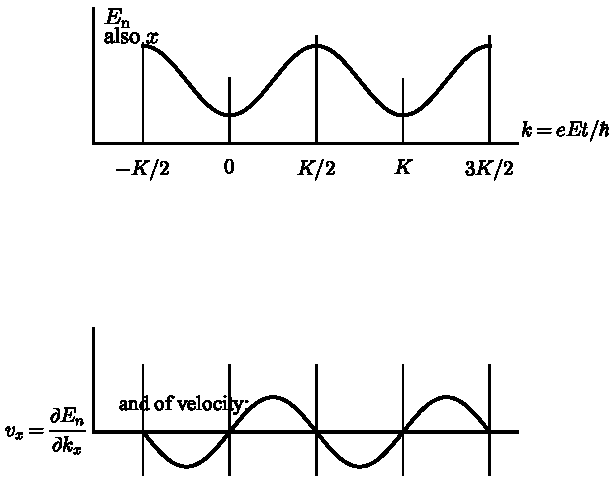
\includegraphics[width=0.72\textwidth]{fig_19.pdf}
\caption*{图 19　$E_n$（亦即位置 $x$）随 $k = eEt/\hbar$ 的周期性变化（横轴标出 $-K/2$、$0$、$K/2$、$K$、$3K/2$），以及速度 $v_x = \partial E_n/\partial k_x$ 随时间的对应周期性变化（原书图注仅作 "Figure 19"）}
\end{figure}

% ---- 原书 p.84 (PDF p099) ----

当 $k$ 增大到区边界时，我们必须利用能带在 $k$ 空间中的周期性。我们看到，$k$ 越过边界后便继续进入下一个区，这恰恰等价于跳回到区的相对面上相应的点。

相当重要的一点是：由此得到的速度是周期性的，既经历负值也经历正值。波包的净位移可以由速度对时间的积分得到：
\begin{align*}
x &= \int_0^t dt\; v_x(t) \\
&= \int_0^t \frac{dt}{\hbar}\,\frac{\partial E_n}{\partial k_x} = \frac{1}{\hbar}\int_0^t \frac{dt}{dk}\,\frac{\partial E_n}{\partial k}\,dk = \frac{1}{eE}\left\{E_n[k_x(t)] - E_n(0)\right\}
\end{align*}

于是每经过一个周期，位移便回到零。这并不奇怪：满带电子必定不携带任何净电流，因为绝缘体正是由满带来描述的。

实际金属或半导体之所以能承载电流，唯一的原因是弛豫效应的存在：电子在 $k$ 空间中才加速了极小的距离，弛豫效应就阻止它们继续完成周期性位移；所得的分布在 $+v$ 方向略有增多、在 $-v$ 方向略有减少，最终结果便是一真实电流。另一方面，在绝缘体中没有可供散射进入的空末态，所以我们必须把电子设想为确实在执行这周期性的位移。

$x$ 方向的总位移是 $W/eE$，即带宽除以 $eE$。这鼓励我们借助一种非常有用的半经典图像来直观想象外势存在下的能带结构（图 20）。半经典地（并非真正经典地，因为能带概念不是经典的）看，固定能量的电子可预期在上、下带边之间来回振荡，被禁带（forbidden gaps）束缚在中间。

\begin{figure}[H]
\centering
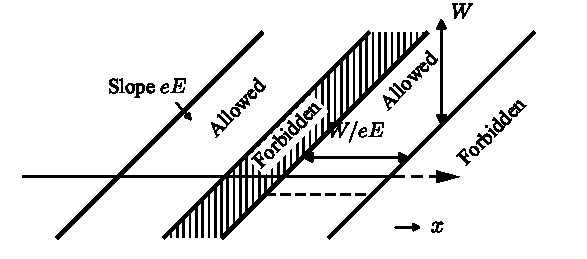
\includegraphics[width=0.72\textwidth]{fig_20.pdf}
\caption*{图 20　外势存在下能带结构的半经典图像：斜率为 $eE$ 的许带（Allowed）与斜纹的禁带（Forbidden）交替排列，带宽为 $W$，固定能量的电子沿水平线在上下带边之间往返，在实空间的总位移为 $W/eE$，横轴为 $x$（原书图注仅作 "Figure 20"）}
\end{figure}

% ---- 原书 p.85 (PDF p100) ----

振荡的总时间周期，就是 $k$ 从一个区边界移动到下一个区边界所需的时间，即 $\hbar K/eE = T$。$K$ 为 $2\pi/a$（$a$ 为晶面间距），因此相应的能量劈裂是 $\hbar\omega = eEa$。这一劈裂的缘由显而易见：一个平移量恰好为 $a$ 的波函数仍满足同一波动方程，而能量的移动量是 $eEa$。这些被 Wannier 称为“Stark 阶梯”（Stark ladders）的能级 (48)，实际上已在 p-n 结中被观测到。即便取相当好的绝缘体中也能达到的正常电场——$10^3$ 到 $10^4$ v/cm，即 10 到 100 esu/cm——这一劈裂也极其微小——$10^{-6}$ 到 $10^{-7}$ ev——对应着极长的周期，量级为 $10^{-8}$ 秒；相比之下，散射的平均自由时间充其量不过 $10^{-11}$ 秒的量级。这就是为什么在有散射存在时，分布通常仍非常接近平衡。另一方面，在 p-n 结中，尤其是在隧道二极管中，人们可以在 10 到 100 个晶格间距上获得带隙量级的电压，此时小的位移便可能对应于相当可观的能量（图 21）。

\begin{figure}[H]
\centering
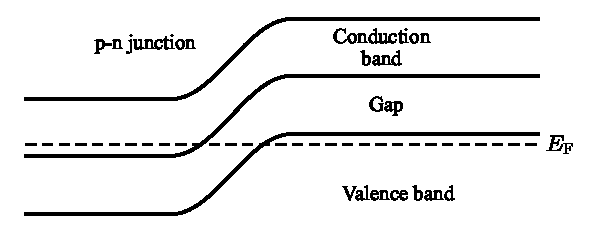
\includegraphics[width=0.72\textwidth]{fig_21.pdf}
\caption*{图 21　p-n 结的能带图：导带（Conduction band）、禁带（Gap）与价带（Valence band）在结区弯曲衔接，虚线为费米面 $E_F$（原书图注仅作 "Figure 21"）}
\end{figure}

这一能量劈裂也可以用一种与"Landau 能级"（Landau levels）劈裂的计算相像得多的方法来计算；Landau 能级在磁场情形中极为重要。假设我们试图用半经典的相位积分（phase-integral）法则，把电子在两条带边之间的往复运动加以量子化：
\begin{equation*}
\int p\,dx = \hbar\oint k\,dx = nh
\end{equation*}
现在让我们取这一轨道与下一个可能轨道之间的差 $\Delta k$：

% ---- 原书 p.86 (PDF p101) ----

\begin{equation*}
2\pi = \oint \Delta k\,dx = \Delta E\oint \frac{\Delta k}{\Delta E}\,dx = \hbar^{-1}\,\Delta E\oint \frac{dt}{dx}\,dx
\end{equation*}
这便直接给出劈裂的 Einstein 频率条件：
\begin{equation*}
\hbar^{-1}\,\Delta E = 2\pi/T
\end{equation*}
$\Delta E$ 我们此前已从别的途径导出，但在磁场情形中，这一方法是唯一简单的方法。

至此，在有效哈密顿量理论的框架之内，自由电子在均匀电场中的行为的讨论便告完成。我们看到，这些现象虽然迷人，却不能为能带结构提供多少信息；所幸磁场的情形在实验上要有用得多 (50)。对这个复杂得多的情形，我将作极为简略的处理，然后试着谈一谈整个有效哈密顿量理论在哪里、又如何失效。

磁场的作用，是把晶体动量方程 $d\mathbf{p}_c/dt = \mathbf{F}$ 中的力 $e\mathbf{E}$ 换成洛伦兹力 $e(\mathbf{v}/c)\times\mathbf{H}$：
% 校注：原书此处印作小写 $dp_c/dt$，与原书 p.83 的 $\mathbf{P}_c$ 同指晶体动量，记号大小写不一致，照录。
\begin{equation*}
\frac{d\mathbf{k}}{dt} = \frac{e}{c}\left[\nabla_{\mathbf{k}}\,E_n(\mathbf{k})\times\mathbf{H}\right] \tag{22}
\end{equation*}
于是，在磁场存在时，$\mathbf{k}$ 沿着一个既垂直于 $\mathbf{H}$、又垂直于能量面梯度的方向移动；这意味着它绕磁场方向描出一条恒能等值线（图 22）。

\begin{figure}[H]
\centering
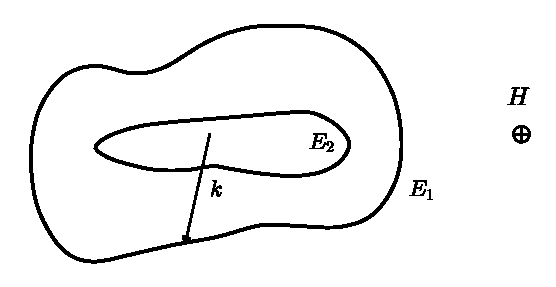
\includegraphics[width=0.72\textwidth]{fig_22.pdf}
\caption*{图 22　磁场中的恒能面与轨道：两条闭合恒能线 $E_1$ 与 $E_2$，$\mathbf{k}$ 沿等能线绕行（箭头），$\mathbf{H}$ 垂直于纸面（图中以 $\oplus$ 标出）（原书图注仅作 "Figure 22"）}
\end{figure}

当 $E_n = \hbar^2k^2/2m^*$ 时，式 (22) 很容易求解，给出回旋频率（cyclotron frequency）$eH/m^*c$。在其它情形下，可以用各种方式证明这一频率为
\begin{equation*}
\Delta E = \hbar\omega_c = \frac{2\pi e}{\hbar c}\,\frac{\partial A}{\partial E}
\end{equation*}

% ---- 原书 p.87 (PDF p102) ----

其中 $A$ 是垂直于场 $\mathbf{H}$ 的适当平面所截出的面积。相应地，在使
\begin{equation*}
A(E) = \frac{2\pi e}{\hbar c}\,n
\end{equation*}
成立的那些能量处，存在着量子化的能级。这些就是 Landau 能级；它们对 De Haas-van Alphen 效应与回旋效应的理论至关重要，而这些效应在实际能带结构的研究中一直极有价值。

式 (22) 的一个重要推论，在过去几年中变得引人注目，特别是通过 Lifshitz 及其在哈尔科夫（Kharkov）的小组的工作。这就是磁场情形中所谓"开放轨道"（open orbits）得以存在的可能性 (51)。能带结构完全可能是这样的：当电子沿恒能面垂直于 $\mathbf{H}$ 漂移时，这个面与区的边界相交，电子便游荡着进入下一个区、再下一个区，如此继续（图 23）。

\begin{figure}[H]
\centering
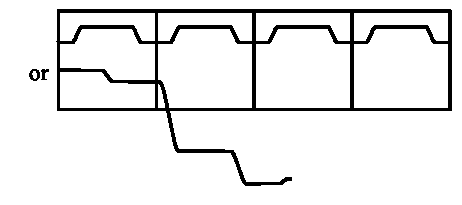
\includegraphics[width=0.72\textwidth]{fig_23.pdf}
\caption*{图 23　开放轨道示意：扩展区图式中的恒能线，"or" 连出两种情形——或者在每个区内闭合，或者穿越一个又一个区边界延伸出去（原书图注仅作 "Figure 23"）}
\end{figure}

这种轨道与电场情形的非常相像；同样，在轨道穿越区边界的那个方向上，电子没有净漂移，但它可以在垂直于 $\mathbf{H}$ 的另一个方向上漂移——处于闭合轨道中的电子则做不到这一点。由于 $1/\omega_c$ 可以做到比 $\tau$ 短——这与电场情形相反——这类轨道可以产生非常强的效应。特别是，它们的存在解释了强场磁阻不饱和这一悬置数十年的难题。

应当强调，所有这些结果不仅受制于有效哈密顿量理论的那些我稍后就要讨论的局限，而且还受制于如下事实：在磁场情形中，除非能量面实际上确是完美的球面或椭球面，否则它们\emph{仅仅}在半经典意义上正确。对于 Si 和 Ge 中能带简并点附近的回旋共振，Fletcher 与 Luttinger (52, 53) 已对量子数非常低的轨道计算并测量了其量子偏离。

% ---- 原书 p.88 (PDF p103) ----

\subsection{“击穿”效应}

有一个物理上理解得相当透彻的效应，完全处于有效哈密顿量的适用域之外，这就是 Zener 隧穿效应（Zener tunneling effect）；它不仅在半导体的实际应用中十分重要，而且可以在一个非常简单的模型上相当容易地加以演示。让我们回到近自由电子的微扰论，讨论若此时施加电场，在区边界处会发生什么。

方程 $\hbar\,(dk/dt) = eE$ 在任何情形下都成立，因此在没有区边界时，电子将在场中无限地加速：
\begin{equation*}
V = \frac{\hbar k}{m} = \frac{\hbar}{m}\left(k_0 + \frac{eEt}{\hbar}\right)
\end{equation*}

事实上，我们可以求得含时波动方程
\begin{equation*}
i\hbar\,\frac{\partial\Psi}{\partial t} = -\frac{\hbar^2}{2m}\,\frac{\partial^2\Psi}{\partial x^2} - eEx\,\Psi
\end{equation*}
的一个精确解，只要令 $\Psi = a(t)\exp\left\{i\left[k+(eEt/\hbar)\right]x\right\}$，便有
% 校注：原书此行指数中印作 (Eet/ℏ)，按 $dk/dt = eE/\hbar$ 及上下文应为 eEt/ℏ，照本意转写。
\begin{equation*}
\left(i\hbar\,\frac{da}{dt} - eEx\,a\right)\exp[i\,k(t)\,x] = \frac{\hbar^2}{2m}\left(k+\frac{eEt}{\hbar}\right)^{\!2}\Psi - eEx\,\Psi
\end{equation*}
此时 $a(t)$ 满足一个带有随时间变化的动能的波动方程
\begin{equation*}
i\hbar\,\frac{da}{dt} = E^0(k(t))\,a = \frac{\hbar^2}{2m}\left(k+\frac{eEt}{\hbar}\right)^{\!2}a
\end{equation*}

这可以积分出来，但其结果相当无关紧要；要紧的是：一旦允许 $k$ 随时间变化，加速运动便可以用一个随时间变化的 $k$ 矢量与动能来代替。

现在让我们引入周期势的 Fourier 分量 $V_K$。这将在波动方程中带来 $k(t)$ 与 $k(t)-K$ 之间的一个常值耦合，后者是另一个同样在不断加速的态。在能量对 $k$ 的图上，$k-K$ 随 $k$ 一同移动；我们既可以把它画在同一条抛物线上，也可以把它画在一条被倒格矢 $K$ 平移、并在区边界处与原抛物线相交的抛物线上（图 24）。在 $V$ 很小的近似之内，只需考虑靠近交叉点 $P$ 的两个 $k$ 矢量。在该点附近，我们可以把正确的波函数展开成这两个加速平面波之和：
\begin{equation*}
\Psi = a(t)\exp\left[i\left(k+\frac{eEt}{\hbar}\right)x\right] + b(t)\exp\left[i\left(k-K+\frac{eEt}{\hbar}\right)x\right]
\end{equation*}

% ---- 原书 p.89 (PDF p104) ----

\begin{figure}[H]
\centering
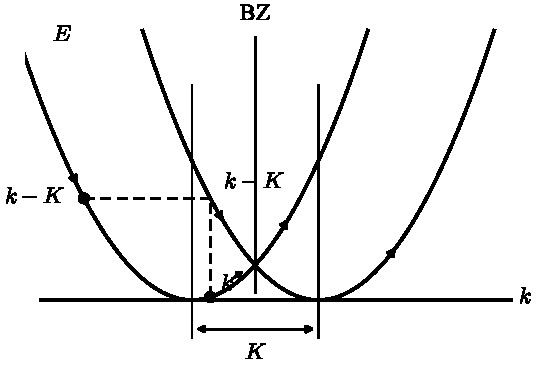
\includegraphics[width=0.72\textwidth]{fig_24.pdf}
\caption*{图 24　Zener 模型的 $E$–$k$ 图：自由电子抛物线与其经倒格矢 $K$ 平移的副本在区边界（竖直的 BZ 线）处交叉；$k$ 与 $k-K$ 两个加速态的轨迹（箭头）沿各自抛物线向上移动，底边双箭头标出间距 $K$（原书图注仅作 "Figure 24"）}
\end{figure}

并且容易看出，我们得到 $a$ 与 $b$ 的一对联立方程：
\begin{align*}
i\hbar\,\frac{da}{dt} &= E[k(t)]\,a + V_K\,b \\
i\hbar\,\frac{db}{dt} &= E[k(t)-K]\,b + V_K\,a
\end{align*}
哈密顿量矩阵是
\begin{equation*}
\mathcal{H} = \begin{pmatrix} E[k(t)] & V_K \\ V_K & E[k(t)-K] \end{pmatrix}
\end{equation*}

这一波动方程的形式是众所周知的，例如在绝热通过或快速通过（adiabatic or rapid passage）的理论中。有两种极限情形：若 $V$ 足够弱，它便仅充当一个小微扰。如果我们从 $a=1$、$b=0$ 出发，则越过区边界后系数 $a$ 仍然很大、$b$ 很小，电子便简单地跳过能隙继续加速。容易证明

% ---- 原书 p.90 (PDF p105) ----

\begin{equation*}
b \simeq \frac{|V_K|^2}{\hbar\,\dfrac{d}{dt}\left(E_k - E_{k-K}\right)}
\end{equation*}

\begin{figure}[H]
\centering
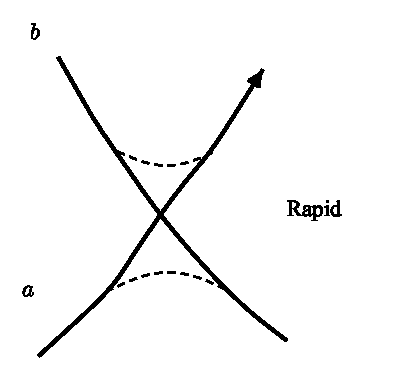
\includegraphics[width=0.72\textwidth]{fig_rapid.pdf}
\caption*{无编号插图（原书不编号，旁注 Rapid）　快速通过极限示意：两支能级交叉，电子由 $a$ 沿原支直接穿过交叉点奔向 $b$（箭头），交叉处的虚线弧示弱耦合引起的微小避免交叉}
\end{figure}

这一情形即所谓的"快速极限"（rapid limit）。

在绝热极限（adiabatic limit）下——此时 $V$ 相当大——更接近正确的假定是：哈密顿量在每一时刻都可以对角化，从而给出两个态的能量，它们分别等价于各自的能带能量 $E_n(k)$。在这种情形中，$a$ \emph{绝热地}（adiabatically）变为 $b$，而跳越能隙的概率极其微小：
\begin{equation*}
P \simeq \exp\left[-\,\frac{|V_K|^2}{\hbar\,\dfrac{d}{dt}\left(E_k - E_{k-K}\right)}\right]
\end{equation*}

\begin{figure}[H]
\centering
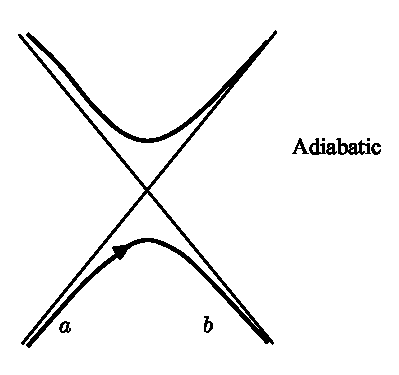
\includegraphics[width=0.72\textwidth]{fig_adiabatic.pdf}
\caption*{无编号插图（原书不编号，旁注 Adiabatic）　绝热通过极限示意：两支能级避免交叉，电子沿下面一支由 $a$ 出发绕过极小值绝热地过渡到 $b$}
\end{figure}

现在
\begin{equation*}
\frac{d}{dt}\left(E_k - E_{k-K}\right) = \frac{2d}{dt}\,\frac{\hbar^2k^2}{2m} = \frac{eE\hbar K}{m}
\end{equation*}
于是
\begin{equation*}
P \simeq \exp\left(\frac{-|V|^2 m}{\hbar^2KeE}\right)
\end{equation*}

这是远为常见的情形。对于 1 伏特的能隙和 $E = 10^4$ v/cm，$P = \mathrm{e}^{-200}$。
% 校注：原书此处印作 "E = 10^4 cm"，单位疑漏 "v/"（对照原书 p.85 的 v/cm 及本段量纲），译文补足为 10^4 v/cm。
而当 $E \sim 10^7$ 时——如 p-n 结中那样——$P$ 相当大，隧穿完全可能发生。

Falicov (54) 最近指出——Blount (55) 则给出了一个好的理论——在磁场情形中，类似的现象在某些晶体中要容易发生得多。如果一条区边界打断了一条近自由电子的磁轨道，那么电子在绕能量面运行时便可以跳入下一条轨道（图 25）。正如我们已经指出的，磁场情形中的运动速率可以变得相当大，而这一效应确实已在 Mg 中被观测到。这一效应称为"磁击穿"（magnetic breakdown）。

% ---- C.4 收尾（原书 p.91 / PDF p106，图 25 之下，协调者补译） ----
值得指出的是，在这个极限下，$E$ 或 $H$ 是以 $\exp[-\mathrm{const}/E\ 或\ H]$ 的形式出现的，因此这些结果绝不可能作为关于 $E$ 或 $H$ 的微扰论的幂级数结果出现，因为 $\mathrm{e}^{-(1/x)}$ 在 $x=0$ 处的一切导数都为零。我们将会发现，有效哈密顿量理论可以被证明在微扰论的\emph{所有阶}上都正确；但当然，我们已经确凿地表明，尽管如此它并不包含全部的物理效应。因此，微扰理论充其量只能渐近收敛。

% 衔接说明：原书 p.91（PDF p106）小节标题之上尚有 C.4（“击穿”效应）的收尾一段
% （“It is worth noting that in this limit ... asymptotically convergent at best.”），
% 按分工自本小节标题起译，该段完全略去。页首的 Figure 25 图身落在 p106，其正文引用
% （“……便可以跳入下一条轨道（图 25）”）已见于 ch2_C34.tex，%FIG 标记置于此处。
% 本小节正文另引 Figure 26、27、28，均出现在本文件范围内，随文标记。
% 本文件末句在原书 p.95（PDF p110）以句号完整结束；p.96（PDF p111）起为第 3 章。

% ---- 原书 p.91 (PDF p106) ----

\begin{figure}[H]
\centering
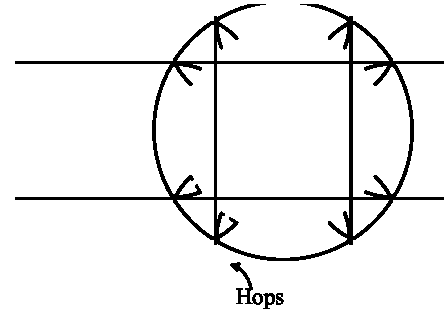
\includegraphics[width=0.72\textwidth]{fig_25.pdf}
\caption*{图 25　磁击穿示意：近自由电子的恒能轨道（圆）被区边界（直线网格）截断，电子绕轨道运行经过交点时跳跃（Hops）进入相邻轨道（原书图注仅作 “Figure 25”）}
\end{figure}

\subsection{有效哈密顿量理论的严格基础}

现在我想简要讨论一下，人们如何着手改进有效哈密顿量理论 (56)。Adams 提出的一个非常简单的定性图像，将以直观的图形方式展示其中的原理。考虑一个非常开放的晶格，其中紧束缚理论是相当好的近似，于是 Bloch 函数就是紧束缚函数，
\begin{equation*}
b^n_k = \sum_j e^{ik\cdot R_j}\,\phi_n(r - R_j)
\end{equation*}
% ---- 原书 p.92 (PDF p107) ----
我们假定交叠相当小，因而在相当好的近似下，$\phi_n$ 也就是 Wannier 函数 $a_n(r - R_j)$。Bloch 波函数实部的图像便可能如图 26 所示。

\begin{figure}[H]
\centering
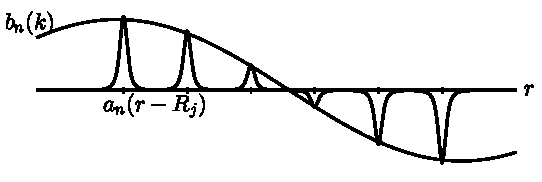
\includegraphics[width=0.72\textwidth]{fig_26.pdf}
\caption*{图 26　紧束缚 Bloch 波函数实部示意：缓变的 $b_n(k)$ 乘以各格点上的 Wannier 函数 $a_n(r - R_j)$（钟形峰），过零后峰反号；横轴为 $r$（原书图注仅作 “Figure 26”）}
\end{figure}

现在，在推导有效哈密顿量时我们做了一个基本假设：$V(r)$——内部场产生的真实微扰——可以用 $V(R)$ 代替，其中 $V(R)$ 由如下关系定义：
\begin{equation*}
V(R)\,a_n(r - R_j) = V(R_j)\,a_n(r - R_j)
\end{equation*}
例如，对均匀电场而言，这意味着 $r$ 可以用相应 Wannier 函数中心处的值代替。于是很容易看出，在我们正在讨论的高度局域情形中，如果 $V(r) = -er$ 是图中所示的线性势，那么 $V(R)$ 就是图 27 所示的阶梯势，而二者之差就是图 28 所示的锯齿波。让我们把这个差记为 $X = r - R$。显然，在任何实际情形中 $X$ 都不会长得像图中那样，但它总可以用这个差来定义，而这个差又依赖于 $a_n(r - R_j)$。我们立刻注意到：

1. 差 $X$ 是 $eEa$ 量级的小量，其中 $a$ 是晶格常数，于是微扰的“大”完全包含在算符 $R$ 之中，从而有效哈密顿量理论本质上包含了所有\emph{大的}效应。

2. $X$ 以晶格周期为周期。因此，在微扰论的任意阶上，我们都可以把 Bloch 函数和 Wannier 函数重新定义为如下\emph{新}能带问题的解：
\begin{equation*}
\mathcal{H} b_k = \left(\frac{p^2}{2m} + V(r) - eEX\right) b_k \simeq {(E^n_k)}'\, b_k
\end{equation*}
% ---- 原书 p.93 (PDF p108) ----
\begin{figure}[H]
\centering
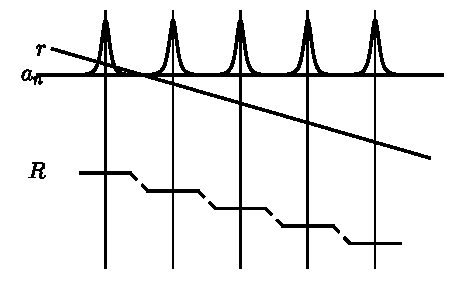
\includegraphics[width=0.72\textwidth]{fig_27.pdf}
\caption*{图 27　强局域情形下的线性势与阶梯势：自上而下依次为各格点上的 Wannier 函数 $a_n$（钟形峰）、线性势 $r$（斜直线）与阶梯下降的 $R$（平台之间以虚线相连），竖直线标记各格点位置（原书图注仅作 “Figure 27”）}
\end{figure}

\begin{figure}[H]
\centering
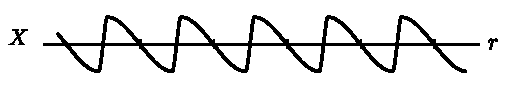
\includegraphics[width=0.72\textwidth]{fig_28.pdf}
\caption*{图 28　差 $X = r - R$ 随 $r$ 变化的锯齿波（原书图注仅作 “Figure 28”）}
\end{figure}

从而消去 $X$ 的效应。这样，在微扰论的任意阶上都存在一组新能带，带有新能量 ${(E^n_k)}'$、新速度（不再严格地由 $\partial E/\partial k$ 给出）等等，而有效哈密顿量理论在附带这一条件的情况下对新能带仍然有效。但要注意，$X$ 是用 $a$ \emph{定义}出来的，而 $a$ 又依赖于 $b_k$，因此求解该方程的唯一办法不是一劳永逸，而是对所有阶逐次迭代。

3. 这种情形下 $X$ 对 Wannier 函数的影响实际上是一个显而易见的物理效应，它确实被我们原有的理论遗漏了：电场不仅必定有加速电子的效应，它还有使单个原子的波函数极化的效应。例如，它必定会把一些 p 带函数混入 s 带中，等等；而且无论 Wannier 函数局域到什么程度，这一效应都必定存在。换句话说，十分明显，$X$ 可以具有带间矩阵元 $X^{nn'}$；但我们预期这些带间矩阵元将是某个周期势的矩阵元，是 $eEa$ 量级的小量。

% ---- 原书 p.94 (PDF p109) ----

讲到这里，这仅仅是一个纲领，而这些结果的实际证明，正是我前面提到的那一组人在过去 10 年里所从事的工作。为了看清必须做些什么，让我们离开紧束缚近似，对一个一般能带来定义 $X$。实际上有两种办法；最显然的一种是用 Wannier 函数来表述：
\begin{equation*}
X\,a_n(r - R_j) = (r - R_j)\,a_n(r - R_j)
\end{equation*}
于是 $X$ 的矩阵元就是
\begin{equation*}
(n, j\,|\,X\,|\,n', j') = \int dr\; a_n(r - R_j)\,a_{n'}(r - R_{j'})\,(r - R_{j'})
\end{equation*}
因此 $X$ 是 $R_j - R_{j'}$ 的函数，这就证明了它是周期的，但非局域。

不那么显然的办法是所谓“晶体动量表象”（crystal momentum representation）。显然，由于
\begin{equation*}
b^n_k(r) = \sum_j e^{ik\cdot R_j}\,a_n(r - R_j)
\end{equation*}
便有
\begin{equation*}
R\,b^n_k = -\,i\,\frac{\partial}{\partial k}\,b^n_k
\end{equation*}
而用另一种表象，
% 校注：按链式法则，此式末项应为 $-i\,e^{ik\cdot r}\frac{\partial}{\partial k}u_k(r)$；
% 原书末项将因子 $-i$ 印漏，此处照原书转录。
\begin{equation*}
-\,i\,\frac{\partial}{\partial k}\,b^n_k(r) = r\,e^{ik\cdot r}\,u_k(r) - e^{ik\cdot r}\,\frac{\partial}{\partial k}\,u_k(r)
\end{equation*}
所以 $X$ 就是单独作用在周期部分 $u_k$ 上的运算 $-i(\partial/\partial k)$。同样，这显然是周期的，因为结果是一个具有同一 $k$ 的 Bloch 函数；但算符是非局域的。这种晶体动量表象在磁场情形中更有价值，因为在那里同样有必要把微扰中出现的算符 $p$ 展开成周期与非周期两部分。

在这两种表象中，每一种都出现一个可能的困难。第一种表象中最为明显：如果 $a_n(r - R_j)$ 局域得不够充分，$X$ 的矩阵元可能很大甚至发散。例如，Wannier 在其原始论文中所算的正是把自由电子当作能带的情形，$a_n$ 仅按 $\sin r/r$ 衰减，因此矩阵元会发散得相当厉害。

绕开这一困难的办法是 Gibson 与 Blount 的贡献。注意我们定义了
% ---- 原书 p.95 (PDF p110) ----
\begin{equation*}
a_n(r - R_j) = \sum_k e^{ik\cdot R_j}\,b^n_k(r)
\end{equation*}
然而，这绝不是唯一的，因为各个 $b_k$ 彼此之间可以带有完全任意的相位，它们只是在相差一个任意常数因子的意义上被定义的。于是我们拥有一个由可能的 $a_n$ 组成的无穷空间：
\begin{equation*}
a_n = \sum_k e^{ik\cdot R_j}\,e^{i\phi_k}\,b^n_k(r)
\end{equation*}
正如 Blount 所证明的，这种相位变换非常像一个规范变换（gauge transformation），多数结果并不因它而真正改变；但方便的做法是以 $a_n$ \emph{尽可能局域}为要求来规定各相位——也就是说，通过一个变分原理。

在 $\partial/\partial k$ 的定义中我们可以看到完全同样的麻烦；同样，每个 $b_n$ 都可以乘以一个任意相位，只有凭借某种特定的选取，我们才能使 $X$ 成为 $k$ 的光滑函数。

在单一、分离的能带情形，可以证明在最佳的相位选取下 $a_n$ 随距离指数式衰减，整个理论收敛得非常好。当出现简并线或简并点时，$a_n$ 衰减得不太快，不过事实上它们衰减得恰好足够快，足以保证收敛。但在这样的点或线上，通过在不同能带之间作新的线性组合，使 Wannier 函数良好局域、$X$ 与 $k$ 算符行为良好，便可以得到简单得多的结果。然而，这时未微扰的能带能量不再是一个数值函数 $E_n(k)$，而是一个矩阵 $E_{nn'}(k)$。这一做法首先由 Luttinger 在处理 Ge 中简并价带顶处的回旋共振（cyclotron resonance）时使用。利用这种相位选取技术，Blount 已经证明了有效哈密顿量理论对微扰论所有阶的有效性。

最后，不妨不再深入细节，对由这些结果可以得到的那种相当迷人的复杂性略作评论。一个重要结果是如下事实：在 $E$ 或 $H$ 的各个阶上，各种物理算符中会进入新的、相当出人意料的项——例如，反常 Hall 效应（anomalous Hall effect）(57) 中著名的反常电流——它可以导致电流、能量输运等等，这些纯粹是量子极化效应，处于正常输运理论的领域之外。当诸如自旋-轨道耦合（spin-orbit coupling）这类进一步的复杂性被恰当地引入时，还会出现许多其他效应，它们复杂但对专家来说饶有趣味。

% 本文件由 scripts/assemble.py 自动装配，勿手改（改 parts/ 后重跑）
% 第3章 元激发

\chapter{元激发}

\section{元激发的概念：多体理论概述}

我在这门课程第一学期中所讲的一切，都建立在一个近似之上——而事实上，我们很容易使自己相信，这个近似在多数情况下是非常粗糙的。那个近似就是：固体中的电子彼此独立地运动，也独立于重离子实（ion cores）的运动——后者我们甚至未曾讨论过。充其量，我们只不过以平均的方式计入了电子之间的相互作用——也就是说，只计到 Hartree-Fock 理论的程度——除了简略地提到 Wigner-Pines 对关联能（correlation energy）的计算之外。

事实上，固体中的电子和离子确实相互作用得非常强烈，而且可以预期是一种急速涨落式的相互作用。有两个简单的例子值得注意。我们已经看到，关联能修正与碱金属的结合能（binding energy）相当，因此很难把它看作一个小效应。我们还注意到，在相当大的距离上，两个电荷之间的相互作用能必须用介电常数（dielectric constant）$\kappa$ 来折减：$\kappa:\ e^{2}/r \to e^{2}/\kappa r$。即便对绝缘体，典型固体的 $\kappa$ 值也在 3 到 20 的量级，因此相互作用由此发生的改变相当可观。

这两者都是真正的多体效应，完全处在 Hartree-Fock 理论的领域之外。在这份讲义的其余部分，我要做的正是讨论这些多体效应。遗憾的是，在这一领域中，除了最高深的专著之外似乎没有一本好的书，尽管其中许多概念并不困难；最好的或许要数 Pines 的一套讲义和重印文集 (58)。其他参考文献有 Landau-Lifshitz（文献 6 的第六章），以及更高深但在高深著作中最易读的 Thouless《Quantum Mechanics of Many-Body Systems》(59)；还有 Les Houches 讲义 (80)。

那么，使用简单的单电子概念，为什么竟能如此经常地给我们带来定性上、有时甚至是半定量上正确的结论呢？这个问题实际上有不少答案，而在接下来的几讲中，我们将主要关心的只是其中之一。不过，在这里把其中几个列举出来或许是有益的：（1）变分定理（variational theorem），（2）不相容原理（exclusion principle），（3）屏蔽（screening），（4）元激发（elementary excitations）的概念。

\subsection{变分定理}

第一个是变分定理，它几乎不言自明——但它只适用于基态能量。这就是说，虽然 Hartree-Fock 波函数对一个包含许多电子和离子的系统来说，并不是其真实波函数的一个十分准确的近似（对大系统而言，两者之间几乎没有任何交叠），但它的能量作为一个近似却远没有那么糟糕。

\subsection{不相容原理}

在电子系统的 Hartree-Fock 理论中，不相容原理在削减多体效应方面起着非常重要的作用。这一效应虽然许多年前就已在自由电子气体中得到认识，但把它明确地指出并加以形式化的，主要是 Weisskopf (61)，其后是处理核子情形的 Brueckner；而有限电子系统中的类似效应，则由 MacWeeny (62) 作了特别的强调。

在 2-A1 节中，我们曾把一个多电子系统的 Hartree-Fock 波函数写成如下形式：
\begin{equation*}
\Psi_{\mathrm{HF}}=\prod_{\substack{\text{occ. states}\\ n,\ \sigma}}^{N}c^{\dagger}_{n\sigma}\ \Psi_{\mathrm{vac}}
\end{equation*}
其中 $c^{\dagger}_{n\sigma}$ 在一组正交轨道 $\phi_{n\sigma}$ 上产生电子；这组轨道是该问题最好的单电子轨道，其含义是：我们消除了所有那种只使单个电子独自从一个占据态 $\phi_{n\sigma}$ 激发到一个未占据态 $\phi_{M\sigma}$（$M>N$）去的矩阵元。正如我们解释过的，这就是方程
$[\mathcal{H},\ c^{\dagger}_{n\sigma}]=E_{n}\,c^{\dagger}_{n\sigma}+\text{truly off-diagonal terms}$
的含义。

于是，能够发生的任何微扰都必须同时把两个电子从占据态 $n$、$n'$ 送到未占据态 $m$、$m'$ 中去；相应的矩阵元是
\begin{align*}
&\left(\,mm'\,\middle|\,e^{2}/r_{12}\,\middle|\,nn'\,\right)\\
&\qquad=\int dr_{1}\int dr_{2}\ \frac{2}{|r_{1}-r_{2}|}\ \phi^{*}_{m}(r_{1})\ \phi^{*}_{m'}(r_{2})\ \phi_{n}(r_{1})\ \phi_{n'}(r_{2})
\end{align*}

例如，微扰论对能量的最低阶修正是
\begin{equation*}
-\sum_{\substack{n,\ n'<N\\ m,\ m>N}}\left|\,\left(mm'\,\middle|\,e^{2}/r_{12}\,\middle|\,nn'\right)\,\right|^{2}\Big/\left(E_{m}+E_{m'}-E_{n}-E_{n'}\right)
\end{equation*}
（译注：求和限第二行原书印作“m, m>N”，第二个 m 漏印撇号，应为 $m, m'>N$。）

由于不相容原理，这些矩阵元很可能相当小。原因在于，态 $m$ 和 $m'$ 必须从与态 $n$ 和 $n'$ \emph{正交}的一个态子空间中选取，因而很可能与它们大不相同——要么在真实空间中占据不同的位置，要么相对它们急速变化，也就是说，处在动量空间的不同部分。于是这个积分通常出人意料地小。有一种很好的表述方式，就是指出：这个积分乃是电荷分布
\begin{equation*}
\rho_{mn}=\phi^{\dagger}_{m}(r_{1})\ \phi_{n}(r_{1})\qquad\text{with}\qquad\rho_{m'n'}=\phi^{\dagger}_{m'}(r)\ \phi_{n'}(r)
\end{equation*}
的 Coulomb 相互作用能。但由正交性，
\begin{equation*}
\int dr\ \rho_{mn}(r)=\int dr\ \rho_{m'n'}(r)=0
\end{equation*}
也就是说，这些电荷分布的符号正负交替，而且通常变化得相当快，所以它们之间的相互作用不很大。这就是 MacWeeny 的论证。

核物理学家则把它表述成：由于不相容原理，电子 $n$ 和 $n'$ 彼此散射所能进入的相空间大受限制。例如，在自由电子气体中，它们必须把彼此完全散射到费米球（Fermi sphere）之外，这就削弱了散射（图 29）。我们在研究费米液体（Fermi liquids）和磁性状态时，都还要回到这个话题。

注意，每一对可能的 $n$、$n'$ 所发生的散射都会是有限的，因此真实的 $\Psi_{\mathrm{g}}$ 相对于 $\Psi_{\mathrm{HF}}$ 来说，对每一个 $n$ 都有一个有限的修改。于是，当 $N\to\infty$ 时，由于 $\Psi_{\mathrm{HF}}$ 是 $N$ 个因子的乘积，而其中每个因子都被修改了一个有限的量，它与真实的 $\Psi_{\mathrm{g}}$ 的交叠 $\to 0$。

\begin{figure}[H]
\centering
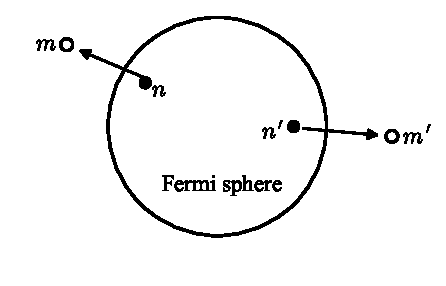
\includegraphics[width=0.8\textwidth]{fig_29.pdf}
\caption*{图 29}
\end{figure}

\subsection{屏蔽}

当我们在电子气体中引入一个电荷——例如，我们可能正在研究其运动的那一个电子的电荷——时，其他电子当然会受它吸引而向它移动（若它为正），或者被它排斥而远离（若它为负）。例如在后一种情形中，这种运动会在原有 Hartree-Fock 密度的基础上留下一处电子电荷的亏缺，它等价于一定量的正电荷。于是，这个外来电子在任何距离上与其他电子相互作用时，就好像它带着一个较小的电荷——它已经被其他电子\emph{屏蔽}了。这一效应非常强地起着削减关联效应的作用。

\subsection{元激发的概念}

最后一个观念，也是我将要用若干页的篇幅来谈的观念，就是元激发的观念。这个概念同样是一个逐渐成长起来的观念，而且成长得如此缓慢，以至于人们几乎说不出它的创始人是谁；不过，对于“存在着这样一种普遍的处理方法”这一自觉的认识，或许 Landau［见 1941 年的文献 (63) 及其著作 (6)］的功劳比任何人都大。“元激发”这个名称就是他引入的。Fröhlich (64) 和 Pines (65) 使人们认识到开发利用量子场论方法的价值，这一做法把多体理论这整个课题开拓成了一门数学学科；而 Kohn (66) 和 Luttinger (67)——连同其他一些人，但他们的贡献超过任何他人——则确立了这样一个观念：元激发理论中的某些思想是可以给出严格证明的。但是，人们不应漏掉 Debye 的名字，他是元激发理论（Debye 声子理论）的第一个使用者；也不应漏掉 Wigner 的名字，他是第一个就关联电子运动这一主题进行推理的人。

元激发概念背后有两个思想。第一个思想是：基态的总结合能并不是一个十分重要的物理量，它与一个物理系统的行为没有多大关系。物理上\emph{重要的}，是较低激发态相对于基态的行为：也就是说，那些在相对较低的温度下或弱的外场中就容易受到激发的态。我们立刻会想到金属或半导体——其中的一切行为都由那些我们说成具有少数几个运动载流子的低激发态所决定；或者想到固体的弹性或热学性质——它们由少数几个我们称之为声子（phonons）的晶格波的存在所决定。因此，我们的兴趣往往集中于一个系统的整组低激发态上，把它视为该系统在物理上最基本的性质。

第二个思想是：低激发态往往——事实上几乎总是——具有特别简单的性质，与其他的态相比，能够以大得多的数学严格性和物理通透性来处理。让我解释一下其中的原因。

正如我一直强调的，尽管有我们一直在谈论的这些削减效应，真实基态 $\Psi_{\mathrm{g}}$ 的波函数和能量所受到的多体修正仍然非常大：特别是 $\Psi_{\mathrm{g}}$ 与单粒子近似 $\Psi_{\mathrm{HF}}$ 之间几乎没有什么关系，甚至毫无关系，因为 $\Psi_{\mathrm{g}}$ 在全部 $N$ 个粒子的坐标上都与后者不同。

不过，关于基态的群性质，我们通常倒是知道一些的。例如在绝缘体中，电子波函数具有平移群的完全对称性：$T\Psi_{\mathrm{g}}=\Psi_{\mathrm{g}}$。

为简单起见，让我们考虑系统恰好只多加了一个粒子的那些激发态。在 Hartree-Fock 近似下，给定晶体动量 $k$ 的最低这样的态，应当是那个多余电子处在最低空带中动量为 $k$ 的状态：
\begin{equation*}
\Psi_{k}=\left(c^{\,n'}_{k}\right)^{\dagger}\ \Psi_{\mathrm{HF}}
\end{equation*}
这当然完全不像一个本征态。然而，我们可以把动量为 $k$、多一个电子的最低本征态 $\Psi_{k}$，与\emph{真实的}基态本征态 $\Psi_{\mathrm{g}}$ 加以比较。会存在某个算符 $q^{\dagger}_{k}$，它代表这两个态之间的关系：
\begin{equation*}
\Psi_{k}=q^{\dagger}_{k}\ \Psi_{\mathrm{g}}
\end{equation*}
关于算符 $q^{\dagger}_{k}$，最重要的一点是：它必然只代表整个系统的一个非常小的位移。在我们正在讨论的简单情形中，我们将看到，事实上在 $N\sim 10^{23}$ 个电子中，只有动量为 $k$ 的那些电子才受到有限大小的扰动。在更复杂的情形中，也许每个电子都在某种意义上被移动了——比如在等离体振荡（plasma oscillation）中那样——但移动的量只是无穷小。

因此，就几乎所有电子而论，$\Psi_{k}$ 与 $\Psi_{\mathrm{g}}$ 几乎是相同的。例如，如果我们考虑一个由靠近中心值 $k_{\mathrm{o}}$ 的那些 $k$ 组成的波包（wave packet），
\begin{equation*}
\Psi_{\text{packet}}(k_{\mathrm{o}},\,r_{\mathrm{o}})=\int\exp\left[-ik\cdot r_{\mathrm{o}}-\frac{1}{2}\left(\frac{k-k_{\mathrm{o}}}{\Delta k}\right)^{2}\right]\Psi_{k}\ dk
\end{equation*}
我们就可以预期，波函数中由此产生的扰动将局限于 $r_{\mathrm{o}}$ 附近尺度为 $1/\Delta k$ 的区域内。如果波函数果真是 Hartree-Fock 的，这当然必然如此：$\Psi_{\text{packet}}$ 将会是
\begin{align*}
\left(\Psi_{\text{packet}}\right)_{\mathrm{HF}}&=\int e^{-ik\cdot r_{\mathrm{o}}}\ \exp\left[-\frac{1}{2}\left(\frac{k-k_{\mathrm{o}}}{\Delta k}\right)^{2}\right]c^{\dagger}_{k}\ \Psi_{\text{H-F}}\ dk\\
&=\int dr\left(\int e^{-ik\cdot(r_{\mathrm{o}}-r)}\ \exp\left[-\frac{1}{2}\left(\frac{k-k_{\mathrm{o}}}{\Delta k}\right)^{2}\right]dk\right)\Psi^{\dagger}(r)\ \Psi_{\mathrm{HF}}\\
&=\left(\int dr\ f_{\text{packet}}(r)\ \Psi^{\dagger}(r)\right)\Psi_{\mathrm{HF}}
\end{align*}
其中
\begin{equation*}
f_{\text{packet}}(r)\propto e^{\,ik_{\mathrm{o}}\cdot(r-r_{\mathrm{o}})}\exp\left[-\left(\frac{\Delta k}{2}\right)^{2}(r-r_{\mathrm{o}})^{2}\right]
\end{equation*}

在更一般的情形中，我们感到，波包的形成将造成对真实基态 $\Psi_{\mathrm{g}}$ 的一个局域性的扰动。于是，算符
\begin{equation*}
q^{\dagger}_{\text{packet}}(r_{\mathrm{o}},\,k_{\mathrm{o}})=\int dk\ \exp\left[-ik\cdot r_{\mathrm{o}}-\frac{1}{2}\left(\frac{k-k_{\mathrm{o}}}{\Delta k}\right)^{2}\right]q^{\dagger}_{k}
\end{equation*}
就是一个只产生局域扰动的算符。

于是，如果我们构造一个带有两个这种波包的波函数
\begin{align*}
&\Psi(k_{\mathrm{o}},\,r_{\mathrm{o}};\ k_{\mathrm{o}}',\,r_{\mathrm{o}}')\\
&\qquad=q^{\dagger}(k_{\mathrm{o}},r_{\mathrm{o}})\,q^{\dagger}(k_{\mathrm{o}}',r_{\mathrm{o}}')\ \Psi_{\mathrm{g}}\qquad\quad k_{\mathrm{o}}\neq k_{\mathrm{o}}',\ \ r_{\mathrm{o}}\neq r_{\mathrm{o}}'
\end{align*}
我们就可以预期，对 $r_{\mathrm{o}}$ 和 $r_{\mathrm{o}}'$ 的大多数可能取值，这两个波包彼此之间不会有多大干涉。于是，如果激发态 $\Psi_{k}$ 的激发能为 $E_{k}=(\Psi_{k}\,|\,\mathcal{H}\,|\,\Psi_{k})-E_{\mathrm{g}}$，我们就可以预期：含有两个这种激发的激发态，其能量是两个能量之和，准确到 $1/N$ 的量级（这正是两个波函数实际交叠的量级）。
\begin{equation*}
E(k_{\mathrm{o}},k_{\mathrm{o}}')=E_{k_{\mathrm{o}}}+E_{k_{\mathrm{o}}'}+\mathrm{O}\left(\frac{1}{N}\right)
\end{equation*}

这就是元激发概念背后的基本思想：在一个非常大的系统中，两个这样的激发将不会相互干涉，无论它们是像我在这里讨论的这种简单准粒子（quasi-particles），还是声子、激子（excitons），抑或是某种更加复杂的东西。因此，当存在的激发数目足够小时，系统的各种性质——特别是能量——将是无相互作用的元激发诸性质的线性叠加。这种情形下的另一个推论是：两个彼此不相互作用的 $q_{k}$ 将具有真实的费米子反对易规则。这一点证明起来并不容易，但它是真的：一般而言，我们总可以把这些 $q$ 取成具有费米子的对易规则。

这样，我们可以对元激发下一个初步的定义：\emph{动量为 $k$ 的元激发，就是那个从基态产生特定类型的、动量为 $k$ 的最低激发态的算符。}根据上面的推理，我们预期这些激发只在弱的程度上相互作用——事实上是 $1/N$ 的量级——因此系统中可以容纳相对大量的这种激发，从而按激发的绝对数目 $n$ 计，系统可以处在激发程度非常高的态，而我们仍然能够把这些激发当作一种近似无相互作用的独立粒子气体来处理。必须认识到，上述波包形成的想法并不限于我所讨论的那种特殊类型的激发态，它也可以应用于那些被适当选取、用以代表单个声子、自旋波（spin waves）等等的最低本征态。换一种说法：元激发的概念，是使系统的方程围绕真实基态——而不是围绕某个独立粒子近似——\emph{线性化}的一种方法。

在进一步讨论上述定义的种种限定与推广之前，最好先给出一些具体的例子。此外，我还想为我早先说过的那个论断提供支持：我们对固体和某些液体的物理分类，在很大程度上取决于它们所表现的元激发的类型。因此，我将用列表的形式写出元激发以及它们在其中显得重要的材料类型：元激发列在左边，它所表征的材料类型列在右边。

\emph{1. 自由电子载流子（free electronic charge carriers）}

\noindent\begin{tabular}{@{}p{0.58\textwidth}@{\hspace{2em}}p{0.36\textwidth}@{}}
a.~有能隙，能量极小值位于动量空间中一些孤立的点附近 & 绝缘体和半导体\\
b.~有能隙，能量极小值位于动量空间中的一个面上；电荷态反常 & 超导体\\
c.~无能隙；$E_{k}$ 在 $k$ 空间中的一个面上变为零 & 金属（正常的）\\
\end{tabular}

\emph{注意：}极化子（polarons）只不过是上列各项的进一步引申，唯有自陷极化子（self-trapped polaron）例外——在某些既非金属又非绝缘体的物质中，它可能成为占主导地位的激发。

\emph{2. 密度波（density waves）}

\noindent\begin{tabular}{@{}p{0.58\textwidth}@{\hspace{2em}}p{0.36\textwidth}@{}}
a.~纵声子（longitudinal phonons） & 固体；量子玻色液体；某些量子费米超流体\\
b.~横声子（transverse phonons） & 固体\\
c.~零声（zero sound） & 某些量子费米正常流体\\
d.~自旋密度波（spin density waves） & 某些量子费米正常流体\\
e.~等离激元（plasmons） & 金属和许多绝缘体——大多数带电的量子流体\\
\end{tabular}

（译注：2a 右栏原书印作“quantum Base liquid”,“Base”应为“Bose”。）

\emph{注意：}经典流体中的普通声和第二声（second sound）都\emph{不是}上述意义上的元激发，而是纯粹的统计现象；它们的存在，依赖于通过不可逆过程建立起局域平衡。

\emph{3. 自旋涨落（spin fluctuations）}

\noindent\begin{tabular}{@{}p{0.58\textwidth}@{\hspace{2em}}p{0.36\textwidth}@{}}
a.~铁磁自旋波：无能隙，$\Delta m=1$ & 铁磁体\\
b.~反铁磁自旋波：有能隙，当 $k\to 0$ 时 $\Delta m\to 0$ & 反铁磁体\\
c.~一般的自旋转动；$k$ 无定义，但仍是元激发理论的一个重要例子 & “磁状态”——铁磁体、反铁磁体和顺磁体\\
\end{tabular}

\emph{4. 其他（miscellaneous）}

\noindent\begin{tabular}{@{}p{0.58\textwidth}@{\hspace{2em}}p{0.36\textwidth}@{}}
a.~激子，包括 Slater 的自旋激发波 & 绝缘体的一种二粒子激发，或许还有超导体\\
b.~旋子（rotons）（有能隙，$k$ 空间中的一个面） & 液态 $\mathrm{He}_{4}$\\
c.~“d-mons” & （在含有两种或多种质量相差悬殊的载流子的物质中，一种其存在性尚成问题的密度波）\\
d.~与周期结构中的各种缺陷相联系的激发——表面态、局域模、杂质态、束缚激子等等。这些是研究细节的人的事情——它们对真实固体的行为可能至关重要，但在多体问题（m.b.p.）中却没有多少基本的重要性。 & \\
\end{tabular}

% ---- A 节收尾（原书 p.104 / PDF p119 顶部，协调者补译） ----
正如你们所见，固态物理学的多数有趣现象都可以在这张清单的某处找到自己的位置。然而并非全部；实际上，甚至并非所有那些与它们共享如下特征的存在物都列于其中：它们是正常固体的规则结构的小尺度、基元性的扰动，而我们在许多方面把它们当作独立粒子来处理。空位、间隙原子与杂质这类存在物，似乎应当另立一个“基元性”（elementaryness）的范畴，它与元激发的观念并不十分相似，主要在于它们的行为在真实的意义上是经典的而非量子力学的。位错，以及它们的“量子”对应物——量子化涡旋与磁通线——则又是另一个范畴；这些是尺度大得多（尺寸 $\sim N^{1/3}$）也更为复杂的现象。

对于每一种元激发类型，上面提到的近似独立性使我们能够用一个共同的进路去计算和理解热学与输运性质。作为零级近似，我们把元激发当作一种无相互作用的 Bose 或 Fermi 粒子气体（视情形而定），于是统计力学与输运理论就变得和完美无相互作用气体的情形一样容易。在更精细的应用中，我们可以把元激发之间的相互作用按任意想要的阶次包括进来；最低阶将允许它们在彼此接近到短距离时相互散射。散射元激发的相互作用，与元激发本身一样，必须被视为实际计算的结果——这种计算必然带入系统的 $N$ 体特征——但在许多情形下我们可以唯象地或近似地处理它，并得到合理的结果。最后，在许多重要情形下，我们甚至可以从元激发的性质出发反推关于基态本身性质的结论，声子零点运动的 Debye-Waller 理论就是一例。

\section{$N+1$ 体问题}

\subsection{准粒子}

让我们来谈谈我们开始这一番讨论时所举的那个特别简单的元激发例子，也就是半导体或绝缘体中的自由载流子。这个问题常常被称作"$N+1$ 体问题"，因为我们真正感兴趣的只是由添加这个额外粒子所带来的那些变化。元激发有两大普遍类型；上面这个例子属于其中被称为"准粒子"（quasi-particles）的那一类——之所以这样称呼，是因为它们非常接近于独立的 Hartree-Fock 单电子波函数中的粒子，而且与它们由之产生的介质中的个别粒子具有相同的对易规则和电荷——在通常情形下，它们是费米子。与之相对照的那一类元激发是集体激发（collective excitation），其中包括声子、等离激元、激子、自旋波等等。$\mathrm{He}_4$ 中的旋子则是一个反常的例子，兼具两种类型各自的性质。

准粒子激发 $q^{\dagger}_{k}$ 的特征在于：它与相应的单粒子近似 $c^{\dagger}_{k}$ 有一个有限的交叠：
\begin{equation*}
\left(q^{\dagger}_{k}\Psi_{\mathrm{g}},\ c^{\dagger}_{k}\Psi_{\mathrm{g}}\right) = Z^{1/2} \tag{1}
\end{equation*}
$Z$ 为有限值（不是 $1/N$ 的量级）。这必须被当作一个定义；我们无法证明这类激发总是存在，而且本来也不应当指望能证明，因为确实存在一些系统，在其中这些激发实际上并不存在。式 (1) 绝非平庸，因为我们当然知道，真实基态 $\Psi_{\mathrm{g}}$ 与 Hartree-Fock 近似 $\Psi_{\mathrm{HF}}$ 之间的交叠是 $e^{-N}$ 的量级。因此，在讨论准粒子时，我们所使用的概念只离开独立粒子模型有限的距离，这是一个巨大的概念上的有利之处。

对式 (1) 的一种思考方式——它同多体理论家实际处理准粒子的方式 (68) 相当贴近——是考虑这样的问题：假设在时刻 $t=0$，我用算符 $c^{\dagger}_{k}$ 作用于真实基态，这个算符（比如说）在一个平面波态 $e^{ik\cdot r}$ 中产生一个粒子。现在我等待一段很长的时间 $T$，在此期间哈密顿量作用于系统，于是 $T$ 时刻的新波函数是 $e^{-iHT}c^{\dagger}_{k}\Psi_{\mathrm{g}}$。现在我要问：粒子是否仍然处在态 $k$ 中？这意味着我施加湮灭算符 $c_{k}$，再与原来的基态作标量积。于是我做如下计算：
\begin{align*}
G_{k}(T) &= \left(e^{-iHT}\Psi_{\mathrm{g}},\ c_{k}\,e^{-iHT}c^{\dagger}_{k}\Psi_{\mathrm{g}}\right)\\
&= \left(\Psi_{\mathrm{g}},\ e^{iHT}c_{k}e^{-iHT}c^{\dagger}_{k}\Psi_{\mathrm{g}}\right)\\
&= \langle g|\ c_{k}(T)c^{\dagger}_{k}(0)\ |g\rangle \tag{2}
\end{align*}
现在，为了求出这个量，一个有益的做法是往这个矩阵元中插入一组严格的激发态，其中之一就是准粒子态 $q^{\dagger}_{k}\Psi_{\mathrm{g}}$；但正如我们说过的，这类态的数目可能非常之大。举例来说，$c^{\dagger}_{k}$ 很可能起到产生这样一个态的作用：它带有两个准粒子和一个准空穴（quasi-hole），三者的动量之和为 $k$：$q^{\dagger}_{k_{1}}q^{\dagger}_{k_{2}}q_{k_{1}+k_{2}-k}\Psi_{\mathrm{g}}$。

让我们把这类可能的激发态中随便哪一个记作 $\Psi_{n}$，并且注意：几乎所有可能类型的 $\Psi_{n}$ 都不是以有限的、而是以无穷小的振幅进入其中，因为具有同一动量的这类态有无穷多个。（唯一可能的例外是周期势中的其他能带态，这个例外处理起来很平凡。）于是
\begin{align*}
G_{k}(T) &= \sum_{m}\ \langle g|c_{k}|m\rangle\ e^{-i(E_{m}-E_{\mathrm{g}})T}\ \langle m|c^{\dagger}_{k}|g\rangle\\
&= Z e^{-iE'_{k}T} + \sum_{n}\ |\langle g|c_{k}|n\rangle|^{2}\ e^{-iE'_{n}T}
\end{align*}
这里已经把激发能 $E'$ 定义为 $E-E_{\mathrm{g}}$。在 $N\to\infty$ 的极限下，对 $n$ 的求和将变成如下形式的一个积分：
\begin{equation*}
\int e^{iE_{n}T}\ dE_{n}\ f(E_{n})
\end{equation*}
其中所有的 $E_{n}$ 都大于 $E_{k}$。这类积分总是导致急速衰减的函数；因此在长时间后的 $G(T)$ 就由那一个准粒子激发所支配。我们可以这样说：在态 $k$ 中产生这个电子之后，经过很长时间，它的 $Z$ 份额仍然留存下来，其余部分则已衰变而进入一个态的连续区；这一份量为 $Z$ 的剩余部分，其行为就好像它具有准粒子的能量一样。

注意，这为我们提供了一种"操作性的"（operational）定义准粒子算符 $q_{k}$ 的办法。也就是说，我们可以使用方程
\begin{align*}
\left(c^{\dagger}_{k}\Psi_{\mathrm{g}}\right)(T) &= e^{-iHT}c^{\dagger}_{k}\Psi_{\mathrm{g}}\\
&= Z^{1/2}e^{-i(E'_{k}+E_{\mathrm{g}})T}\ q^{\dagger}_{k}\Psi_{\mathrm{g}} + \int dE_{n}\ e^{-i(E'_{n}+E_{\mathrm{g}})T}\ f(E_{n})\Psi_{n}
\end{align*}
将此式乘以 $e^{i(E'_{k}+E_{\mathrm{g}})T}$ 并积分，得到
\begin{equation*}
q^{\dagger}_{k}\Psi_{\mathrm{g}}\ \propto \int_{0}^{\infty} dT\ e^{i(E'_{k}+E_{\mathrm{g}})T}\left(c^{\dagger}_{k}\Psi_{\mathrm{g}}\right)(T)
\end{equation*}
或者
\begin{equation*}
q^{\dagger}_{k} = \text{const.}\ \int_{0}^{\infty} dT\ e^{i(E'_{k}+E_{\mathrm{g}})T}\ c^{\dagger}_{k}
\end{equation*}
这就是说，我们只需对所有时间作适当的平均，就能从含时波函数中挑出属于真正准粒子的那一部分；这样做所给出的严格准粒子函数，比起任何背景成分来要多出无穷多倍。用能谱的语言来说，我们可以画出图 30。于是，如果乘上一个形如 $\int_{0}^{\infty}dT\ e^{-iET}$ 的能量 $\delta$ 函数滤波器，我们就能容易地把准粒子态及其能量挑出来。

\begin{figure}[H]
\centering
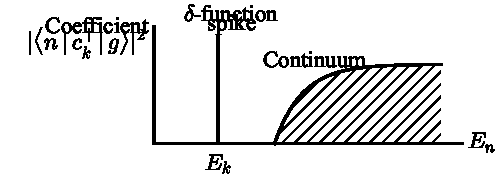
\includegraphics[width=0.72\textwidth]{fig_30.pdf}
\caption*{图 30}
\end{figure}

这种通过研究 $T\to\infty$ 极限下的行为来获得严格结果的技巧，是多体理论（M. B. T.）的一种特征性的形式工具。Kohn、Ambegaokar (69) 以及晚近的 Blount (45) 基于这些思想，已经就 $N+1$ 电子问题确立了大量严格结果。其中一个结果是严格地证明：在与单能带近似等价的理论中，可以把准粒子能量曲线 $E(k)$ 用作单能带哈密顿量中有效的动能部分，正如在 Bloch 电子理论中可以把哈密顿量处理成 $E(k)+V(R)$ 那样。另一个结果是证明：在长程极限下，势要被宏观的静态介电常数 $\kappa$ 所修正；当电子离电荷足够远时，它会以势 $eq/\kappa r$ 被一个静止电荷 $q$ 吸引。

这最后一个结果在文献中受到了极大的关注。虽然从物理观点来看它是平凡的，但数学上的论证却并非如此，而且它还揭示出一些有意思的东西。我在本课程中无法给出完整的推导，但我认为，粗略地展示一下其中牵涉到哪些东西，对于领会 $N+1$ 体问题的处理技巧是有教益的。

假设在材料中建立起了一个静电势 $V(r)$——比如说，通过引入外电荷 $e$——它当然会在哈密顿量中给出一个微扰项
\begin{equation*}
\int dr\ \Psi^{\dagger}(r)V(r)\Psi(r) = \frac{1}{N}\sum_{q,k}\ c^{\dagger}_{k+q}c_{k}\ V(q) \tag{3}
\end{equation*}
其中
\begin{equation*}
V(q) = \frac{1}{\Omega}\int dr\ e^{iq\cdot r}V(r) = \frac{4\pi e}{\Omega q^{2}}
\end{equation*}
这是对一个外电荷 $e$ 而言的。

我们在这里假定，引入电荷时离子实并不移动，因此势不会按相应于离子实运动的介电常数而折减；这在非极性半导体中是合理的，而在其他情形下这个效应无论如何也总可以被考虑进去。

式 (3) 取在两个准态（quasi-states）$K$ 与 $K+Q$ 之间的一个典型矩阵元是
\begin{equation*}
\left(\Psi_{K'},\ \sum_{k}c^{\dagger}_{k+Q}c_{k}\ \Psi_{K+Q}\right)V(Q) = M_{K}(Q)V(Q)
\end{equation*}
其中显然，一切 $q\neq Q$ 的矩阵元都必定因动量守恒而消失。Kohn 和 Ambegaokar 的定理是：该方程中的标量积等于 $1/\kappa$，这里 $\kappa$ 是电子气的介电常数——至少在 $Q\to 0$ 的极限下是如此，这一极限对应于非常长程的力［$V$ 的长程部分当然就是 $V(Q\to 0)$］。

这个定理乍看起来相当令人惊讶，因为恰恰在 $Q=0$ 的极限下，矩阵元 $\left(\Psi_{K},\ \sum_{k}n_{k}\ \Psi_{K}\right)$ 就等于粒子总数，即 $N+1$。

然而，出现这个分歧的原因是清楚的：单个准粒子所引起的扰动含有一些本质上是长程的成分，因为那个电子的电荷会把整个晶体一直极化到 $r\to\infty$，而这种长程效应在 $Q\to 0$ 的极限下导致奇特的行为。这确实是原因所在，而这一点可以用一种非常直接的办法来证明。让我们考察一个完整绝缘体的样品，往其中加入一个单独的电子——不是让它处在某个特定的准粒子态 $K$ 中，而是处在我早先提到过的那种波包（wave packet）中：它由围绕某一给定的 $K_{\mathrm{o}}$ 的那些态的线性组合构成，并且局域在一点 $R_{\mathrm{o}}$ 附近，我们将选取这一点作为原点：
\begin{equation*}
\Psi_{R_{\mathrm{o}}=0,\ K_{\mathrm{o}}} = \frac{\text{const.}}{\left[N(\Delta K)^{3}\right]^{1/2}}\ \sum_{K}\ e^{-\frac{1}{2}(K-K_{\mathrm{o}})^{2}/(\Delta K)^{2}}\ \Psi_{K} \tag{4}
\end{equation*}

让我们先从物理上看一看这个问题。我们已经在绝缘体的中心加入了一个额外的电子，它处在一个大小为 $\Delta R\approx 1/\Delta K$ 的区域内（图 31）。因此我们认为，在这个区域内有一份额外的电子电荷。现在，如果我们考虑由此造成的、从 $\Delta R$ 一直到样品外半径 $R$ 的那一层电介质球的极化，那么这个球将被电子电荷的电场 $E$ 所极化，极化强度为 $P=[(\kappa-1)/4\pi]E$。这就导致该球内、外表面上的总面电荷为
\begin{align*}
&+\ (\kappa-1)(\Delta R)^{2}E(\Delta R)\qquad\text{inner}\\
&-\ (\kappa-1)R^{2}E(R)\qquad\qquad\ \ \text{outer}
\end{align*}
而 $E$ 是由净电荷造成的场：
\begin{equation*}
E(\Delta R) = \frac{e-(\kappa-1)(\Delta R)^{2}E(\Delta R)}{(\Delta R)^{2}}
\end{equation*}
或者说 $Er^{2}=e/\kappa$，而面电荷为 $\pm[(\kappa-1)/\kappa]\ e$。

\begin{figure}[H]
\centering
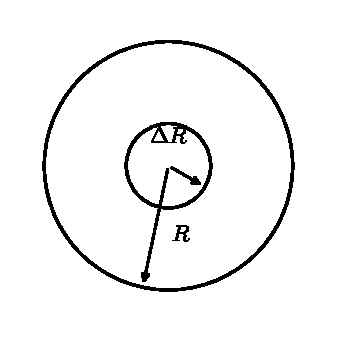
\includegraphics[width=0.72\textwidth]{fig_31.pdf}
\caption*{图 31}
\end{figure}

实际上，球并不会在 $\Delta R$ 处的边界上被物理地切开，因此这个面电荷将近似地被内层介质球表面上的面电荷所补偿。极化电荷的实际位置只能粗略地指明为处在准粒子所在的地方。我们所能确切断定的只是：电子电荷中有 $(\kappa-1)/\kappa$ 的份额出现在球的外表面上，只有 $1/\kappa$ 的份额留存下来，从而能够与任何局域地插入的外来电荷 $q$ 相互作用。

这是所有涉及可极化介质中载流子的问题所共有的一种奇特现象的一个特别简单的例子：运动电荷中总有一个相当可观的份额实际上是处在样品表面上的。事实上，在金属中——那里 $\kappa(q\to 0)=\infty$——原则上全部电荷都在表面上；在电介质中则只有 $(\kappa-1)/\kappa$。换一种说法：那个无限长程的、$Q=0$ 的项总是表现出反常的、不连续的行为。我们也可以把它解释为一种屏蔽效应——至少部分地是如此；在长距离上，电子与其他电荷的相互作用势被削减了一个因子 $\kappa$。

还有待于指出这些事实与 Kohn-Ambegaokar 恒等式之间的关系，该恒等式涉及矩阵元
\begin{equation*}
\lim_{Q\to 0}M_{K}(Q) = \lim_{Q\to 0}\sum_{k}\left(\Psi_{K'},\ c^{\dagger}_{k+Q}c_{k}\ \Psi_{K+Q}\right) \tag{5}
\end{equation*}
注意，这个量如同常数 $Z^{1/2}$ 一样，是准粒子量与裸粒子（bare-particle）量之间的一个"交叉"标量积。事实上，它恰恰类似于量子场论中的"顶点重整化常数"（vertex renormalization constant），正如 $Z$ 之于该理论中的"波函数重整化"常数 $Z$。（译注：末句中前一个 $Z$ 原书即印作 $Z$，按上文的类比关系，疑应为 $Z^{1/2}$。）

我们通过计算一个包含 $\Delta R$ 球的球体内的电荷来求式 (5)，准粒子就处在 $\Delta R$ 球之内。引进一个光滑函数 $f(r)$，它在 $r=\Delta R$ 处等于 1，而在某个半径 $R_{1}$ 处下降到零，其中 $R\gg R_{1}\gg\Delta R$。于是，半径为 $R_{1}$ 的球体内的电荷由下式给出：
\begin{equation*}
e\left(\Psi_{R_{\mathrm{o}}=0,\ K_{\mathrm{o}}}\ \int dr\ f(r)\Psi^{\dagger}(r)\Psi(r)\ \Psi\right) \tag{6}
\end{equation*}
（译注：左端 bra 态的下标原书印作 $k_{\mathrm{o}}=0$；按式 (4) 及下文"$\Psi(R=0)$"的表述，应为 $R_{\mathrm{o}}=0$。）

让我们对这个表达式作 Fourier 分析，利用
\begin{equation*}
\Psi^{\dagger}(r)\Psi(r) = \sum_{Qk}\ e^{iQ\cdot r}\ c^{\dagger}_{k+Q}c_{k}
\end{equation*}
以及波包 $\Psi(R=0)$ 的 Fourier 展开式 (4)。式 (6) 成为
\begin{align*}
\frac{e\times\text{constants}}{(\Delta K)^{3}N}\ &\sum_{K,K',k,Q}\ \left(\int dr\ f(r)\,e^{iQ\cdot r}\right)\left(\Psi_{K'},\ c^{\dagger}_{k+Q}c_{k}\ \Psi_{K}\right)\\
&\times\exp\left[-\frac{1}{2}\left(\frac{K-K_{\mathrm{o}}}{\Delta K}\right)^{2}-\frac{1}{2}\left(\frac{K'-K_{\mathrm{o}}}{\Delta K}\right)^{2}\right]
\end{align*}
（译注：矩阵元中 ket 的下标原书印作 $K'$；按下文"动量守恒要求 $K'=K+Q$"的叙述，应为 $K$。）

现在，
\begin{equation*}
\int dr\ f(r)e^{iQ\cdot r} = f(Q)
\end{equation*}
$f(Q)$ 有三个重要的性质：(a) $f(Q=0)=(4\pi/3)R_{1}^{3}$，即 $f(r)$ 的"体积"；(b) $f(Q>1/R_{1})\simeq 0$，因而 $f(Q)$ 在 $Q$ 空间中比 $\Delta K$ 陡峭得多地成峰，并且 $f(\Delta K)\simeq 0$；(c) $\sum_{Q}f(Q)=1$。动量守恒要求 $K'=K+Q$，于是性质 (b) 使得指数因子恰好就是
\begin{equation*}
\exp\left[-\left(\frac{K-K_{\mathrm{o}}}{\Delta K}\right)^{2}\right]
\end{equation*}
我们预料，由于 $K$ 与 $K_{\mathrm{o}}$ 非常接近，而矩阵元
\begin{equation*}
M_{K}(Q)
\end{equation*}
没有理由随 $K$ 急速变化，所以我们可以在假定 $M_{K}$ 为常数的情形下完成对 $K$ 的求和：
\begin{equation*}
(6) = e\sum_{Q}\ f(Q)\,M(Q)\ \sum_{k}\ \frac{\text{const.}}{N(\Delta K)^{3}}\ \exp\left[-\left(\frac{K-K_{\mathrm{o}}}{\Delta K}\right)^{2}\right]
\end{equation*}
而这个求和恰恰就是波包的归一化和。于是，电荷表达式 (6) 就变成正好是 $e\sum_{Q}f(Q)M(Q)$。正如我们已经指出的，在 $Q$ 恰好为零时
\begin{equation*}
M(0) = N + 1
\end{equation*}
因此电荷中有一项贡献恰好是
\begin{equation*}
\frac{4\pi R_{1}^{3}}{3}\ e\ (N+1)
\end{equation*}
这一项贡献所代表的，只不过是整个电子气的平均电荷中包含在 $R_{1}$ 球内的那一部分，它当然必须恰好被离子背景电荷所补偿。电荷的这一部分很容易辨认，因为它与波包毫无关系——它会随 $R_{1}$ 无限增大。事实上，可以证明：即使把波包从 $R_{1}$ 球内移走，这一部分也不受影响。因此它纯粹是一个平凡的背景效应。

如果我们令 $M(Q\neq 0)=$ 常数 $M$——这是十分合理的——那么剩下的电荷就是
\begin{equation*}
eM\sum_{Q}\ f(Q) = eM
\end{equation*}
% ---- B.1 收尾（原书 p.112 / PDF p127 顶部，协调者补译；承接上式 eM Σ f(Q) = eM） ----
（由性质 (c)）；于是它与半径 $R_1$ 无关，正是直接与波包自身相联系的那份电荷。正如我们的物理推理早已告诉我们的，它恰好就是 $e/\kappa$。这样，我们就得到了 Kohn 恒等式的一个物理上的——尽管显然不是严格数学意义上的——证明。实际的证明看来只能借助图微扰论（diagrammatic perturbation theory）来进行。应当认识到：整个 $N{+}1$ 体理论的这套机制确实只在微扰论的界限之内被严格证明——尽管恰恰在这个情形下，我们完全有理由相信微扰论实际上收敛，并且准确地代表了物理实在。

Blount 为此补充了一个颇有意思的结果。实质上，我们迄今为止所做的，正相当于 Bloch 电子的零阶单带理论——亦即有效哈密顿量理论
\begin{equation*}
\mathcal{H} = E(\mathbf{k}) + V(\mathbf{R})
\end{equation*}
Blount 指出，只要把 $N{+}1$ 体波函数 $\Psi_{\mathbf{k}}$ 本质上取作
\begin{equation*}
\Psi_{\mathbf{k}}(\mathbf{r}_1,\ \mathbf{r}_2,\ \ldots\,,\mathbf{r}_{N+1})\ =\ \left\{\mathrm{e}^{i\mathbf{k}\cdot\mathbf{r}_1}\ U_{\mathrm{o}}^{\mathbf{k}}\left(\mathbf{r}_1\ldots\mathbf{r}_{N+1}\right)\right\}\ \text{的反对称化}
\end{equation*}
其中 $U_{\mathrm{o}}^{\mathbf{k}}$ 是其 $N{+}1$ 个粒子变量的完全周期函数，就可以得到 $N{+}1$ 体问题的完整理论。于是 $U_{\mathrm{o}}^{\mathbf{k}}$ 的处理方式与通常波函数的 Bloch 部分十分相像，并且由它出发——利用 Kohn 与 Ambegaokar 的恒等式——例如可以导出关系式
\begin{equation*}
V(\mathbf{r}) = \frac{1}{\kappa}\,V(\mathbf{R})\ +\ \text{量级为}\ \frac{\partial V}{\partial \mathbf{R}}\cdot a\ \text{的修正项}
\end{equation*}
然而，这些修正项与真实单电子情形的修正项颇为不同——这是意料之中的，因为现在 $V$ 既能极化原子芯，也能极化所加入电子的波函数。

\subsection{$N+1$ 体问题中声子的效应}

在以上全部讨论中，我们一直仿佛假定多体系统里只有价带中的电子可以自由运动。这一假设基于
Born-Oppenheimer 绝热近似；按照该近似，由于原子核与电子的质量相差极大，原子核的一切运动
相对电子而言都无限缓慢。对于为之发明的有限分子体系，这个近似非常好，因为其中电子激发能
从而其频率确实远高于离子的相应量，所以离子可以认为是静止的；但它当然恰恰会在我们觉得最
有意思的那个区域完全失效，即固体最低能量激发的区域，因为在这里我们无法\emph{先验地}断定
电子能量相对离子能量究竟是大还是小。

固体中在这里有任何重要性的离子运动，可以用离子实绕其平衡位置振动的量子化波动来描述
（图 32）。正如各位所知，这些量子化的波称为声子（phonon）。

\begin{figure}[H]
\centering
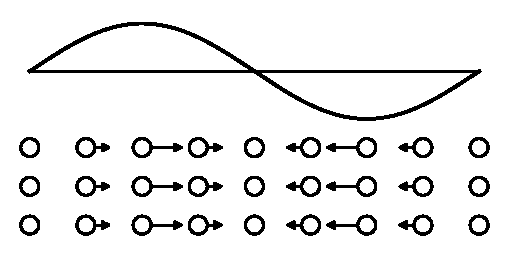
\includegraphics[width=0.72\textwidth]{fig_32.pdf}
\caption*{图 32}
\end{figure}

它们本身就是固体的元激发；事实上，它们是最早被发现的一组元激发——由 Einstein 和
Debye 在 1910 年前后发现。尽管如此，让你可能感到意外的是，把声子当作固体的多体集体激发
来处理时，仍有许多重要问题悬而未决。不过眼下我们只关心声子对我们一直在讨论的准粒子激发
性质的修正。

正如各位所知，对于每个 Bravais 原胞只含一个原子的固体，声子谱有三支，在长波长和简单
晶体取向下退化为一支纵波和两支横波声波；长波情形下频率由 $\omega_{k}=c_{l}k$ 或
$c_{t}k$ 给出，$c$ 为纵向或横向声速；能量为 $\hbar\omega_{k}$。

更复杂的固体的声子谱还有三支或更多的"光学"支，在长波长下退化为 Bravais 原胞内不同
原子彼此相对的运动；而在两个原子并不相同的情形下，

\begin{equation*}
(\text{Na})^{+}\!\to\;\; \leftarrow\!\!(\text{Cl})^{-}
\qquad\quad
(\text{Na})^{+}\!\to\;\; \leftarrow\!\!(\text{Cl})^{-}
\end{equation*}

单位体积便带有相应的偶极矩 $\mathbf{P}$。稍后我们会讨论到，在光学支中，纵波与横波的频率
在无限长波处相差一个有限量 $\omega_{lo}-\omega_{to}$。于是我们在图 33 中草绘了单原子
晶格和离子性双原子晶格的声子谱。

\begin{figure}[H]
\centering
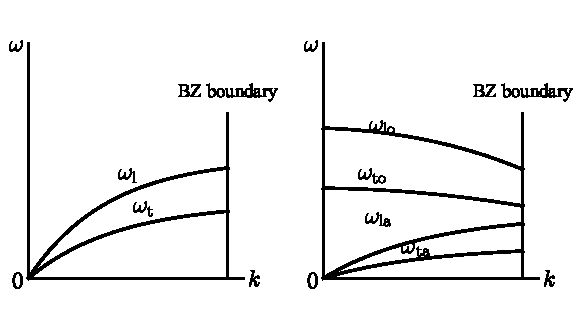
\includegraphics[width=0.72\textwidth]{fig_33.pdf}
\caption*{图 33}
\end{figure}

声子的存在显然会带来若干后果。首先也是最简单的一点：我们看到，准粒子态不再必然是具有
给定动量或 $k$ 矢量的最低能量激发态；事实上，相对声子态而言，它通常将是一个能量非常高的
态。这正是我们在定义元激发时加以限定、要求激发态属于\emph{某一特定类型}的原因。就准粒子
与声子相对照的情形而言，区分其实相当容易，因为准粒子算符是费米型的，它使电子数目改变
1，即从 $N$ 变到 $N+1$，而产生声子的算符 $b_{\mathbf{K}}^{\dagger}$ 则近似是玻色型的，
既不改变离子数也不改变电子数；但一般说来区分并非如此简单。例如，态 $q_{k}^{\dagger}\Psi_{N}$
的能量未必低于带有一个声子加一个准粒子激发的态
$q_{k-\mathbf{K}}^{\dagger}b_{\mathbf{K}}^{\dagger}\Psi_{N}$；两个算符都是费米型的，
两个态都是 $N+1$ 粒子态。

当我们引入电子-声子相互作用的概念时，一个严重得多的问题出现了。这一相互作用有两种效应：
\emph{散射}与\emph{极化}。不过在讨论这些效应之前，我想先就电子-声子相互作用本身说几句话。

为了对这个相互作用可能取的形式获得一些概念，让我们在一个简单近似下把它计算出来。有一种
办法非常简单，但必须谨慎对待，这就是所谓的"刚性离子"（rigid-ion）模型。在此我们假定，
电子与之相互作用的晶格势是每个离子各自贡献之和：$V(r)=\sum_{j}V(r-\mathbf{R}_{j})$，或者
写成电子的二次量子化形式
$V=\int\mathrm{d}r\,\sum_{j}V(r-\mathbf{R}_{j})\,\Psi^{\dagger}(r)\Psi(r)$。我们为电子选用的
未微扰波函数，是在把 $\mathbf{R}_{j}$ 固定在格点上时算出的；于是微扰必定来自 $\mathbf{R}_{j}$
的位移 $\delta\mathbf{R}_{j}$，它由声子的存在引起：

\begin{equation*}
\mathcal{H}' \;=\; \sum_{j'} \int \mathrm{d}r\;\; \delta\mathbf{R}_{j} \cdot \nabla V(r-\mathbf{R}_{j})\, \Psi^{\dagger}(r)\, \Psi(r)
\end{equation*}

（译注：原书求和指标印作 $j'$，而式内各下标均为 $j$，两者应统一。）

$\delta\mathbf{R}_{j}$ 可以用声子振幅 $Q_{\mathbf{K}}$ 展开：

\begin{equation*}
\delta\mathbf{R}_{j} \;=\; \text{const} \cdot \sum_{\mathbf{K}} \mathrm{e}^{-i\mathbf{K}\cdot\mathbf{R}_{j}}\, Q_{\mathbf{K}}
\end{equation*}

而各个 $\Psi$ 则用 Bloch 函数展开：

\begin{align*}
\mathcal{H}' = {} & \int \mathrm{d}r \sum_{\substack{nn'k \\ k'\mathbf{K}j}}
\mathrm{e}^{-i\mathbf{K}\cdot\mathbf{R}_{j}}\,
\mathrm{e}^{ik\cdot r}\, u^{n*}_{k}(r)\,
\mathrm{e}^{-ik'\cdot r}\, u^{n'}_{k'}(r) \\
& \times\; Q_{\mathbf{K}}\, c^{n\dagger}_{k}\, c^{n'}_{k'} \cdot \nabla V(r-\mathbf{R}_{j}) \\
= {} & \sum_{k\mathbf{K}nn'} M^{nn'}_{k,\mathbf{K}}\, Q_{\mathbf{K}}\, c^{n'\dagger}_{k+\mathbf{K}}\, c^{n}_{k}
\end{align*}

其中

\begin{equation*}
M^{nn'}_{k\mathbf{K}} \;=\; \text{const.} \int \nabla V(r-\mathbf{R}_{j})\, \phi^{n}_{k+\mathbf{K}}(r)\, \phi^{n'}_{k}(r)\;\, \mathrm{d}\Omega_{\mathrm{cell}}
\tag{7}
\end{equation*}

$Q_{\mathbf{K}}$ 又可以用声子的产生与湮灭算符 $b_{\mathbf{K}}$ 和 $b_{-\mathbf{K}}^{\dagger}$
表出。这样一来，相互作用就具有电子被散射同时产生或湮灭一个声子的形式（图 34）。

\begin{figure}[H]
\centering
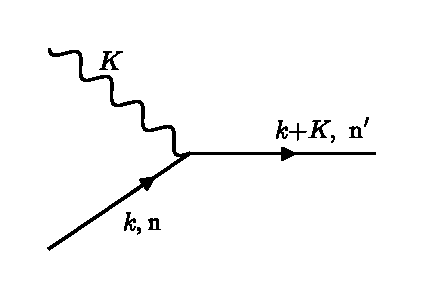
\includegraphics[width=0.72\textwidth]{fig_34.pdf}
\caption*{图 34}
\end{figure}

比这个相当朴素的模型更为认真的分析其实是可以做出的；关于这些分析的精彩论述，我向各位
推荐 Ziman 的书（文献 (3)）中相应的章（第五章）。这里我只想集中讨论一个极限情形，即
$k$ 很小的情形。

查阅 Ziman 的书可以发现，在这个极限下矩阵元 $M$ 结果正比于 $\mathbf{K}$，于是相互作用
并不像乍看之下那样正比于离子的位移 $\delta\mathbf{R}_{j}\propto Q_{\mathbf{K}}$，而是正比于
其应变（或称"形变"）$\nabla\mathbf{R}_{j}\propto\mathbf{K}Q_{\mathbf{K}}$（译注：原文如此，
按本意应为 $\nabla\,\delta\mathbf{R}_{j}$）。在单电子理论范围内证明这一点并不十分困难，但
有趣的是要证明它在一般情形下也成立，即使把多体效应考虑进去。

这非常值得去做，因为脱离价带电子来谈论离子和离子实自身的位移是没有意义的——至少在某种
意义上，这些电子是随它们一起被携带的。撇开别的不论，我们至少意识到：由于离子实带有净电荷，
当它们形成长波长的纵波时，会在波峰处积累起非常大的空间电荷，这种电荷必然要移动价电子的
电荷分布。一般地说，"价电子气整体不随离子运动"这一假设显然站不住脚，这一点是明显的。
因此，电子-声子相互作用中有相当大的部分必须被认为已经包含在声子激发本身的定义之中，正如
被散射的电子其实并不是单个的独立电子，而是准粒子一样。

这个问题与场论中的重整化问题极为相似；我们看到的"物理"准粒子和声子，与我们能够简单
设想的"裸"粒子全然不同，其实验性质——能量、相互作用等等——包含了围绕裸粒子的扰动云的
贡献。在固体理论中，我们并没有场论中那种不可挽回地阻止我们找出"裸"性质与"物理"性质之间
真实关系的发散；尽管如此，固体是如此复杂的对象，以致为了求出的不仅有声子频率和准粒子
能量、还有它们之间的相互作用，求诸实验往往比求诸理论更有用。这就是\emph{形变势}
（deformation potential）理论（文献 (70)）背后的思想。在这一理论中，我们借助均匀应变的
可观察（至少原则上可观察）效应来估计长波长声子的效应。

于是设想，为简单起见，我们有一块绝缘体，并以某种相当平滑的方式使它发生弹性形变，于是，
若各处的局域位移为 $\delta\mathbf{R}_{j}$，则任一局域区域内都有明确定义的局域压缩
$\Delta=\nabla\cdot\delta\mathbf{R}_{j}$，并且在愿意的话还有切应变
$S=\operatorname{symm}\bigl\{\nabla\,\delta\mathbf{R}_{j}-\tfrac{1}{3}\,\nabla\cdot(\delta\mathbf{R}_{j})\,\mathbf{1}\bigr\}$。
我们让 $N$ 体电子气完全绝热地随之形变。于是，在新的、已形变的晶格中，我们可以构建一个
波包 $\Psi_{\text{packet}}(k_{0},r_{0})$，其中心动量为 $k_{0}$，位于围绕 $r_{0}$、尺度为
$1/\Delta k$ 的区域内。假定该区域内的形变 $\Delta$、$S$ 相当均匀；否则，晶格当然就不再
足够周期，我们也就无法在不确定度 $\Delta k$ 之内定义波矢 $k_{0}$。这个由精确准粒子构成的
新波包具有新的能量 $E^{\prime}_{n}(k_{0})$，它与原来的能量不同，因为晶格在局域上发生了
形变；若无形变，显然无论原子的\emph{位移}有多大，能量都根本不会改变。由于声子中原子的
运动相当小，可以合理地预期带能量对形变是线性的，其线性比例常数称为"形变势"常数 $E$：

\begin{equation*}
E^{\prime}_{n}(k_{0}) \;-\; E_{n}(k_{0}) \;=\; E_{\Delta}(k_{0})\,\Delta \;+\; E_{S}(k_{0})\, S \;+\; \cdots
\tag{8}
\end{equation*}

这一\emph{以经验方式定义的}势，就是准粒子 $q_{k}^{\dagger}$ 的真实散射势，它既包括形变给
$\Psi_{g}$ 带来的近乎无穷的改变，也包括准粒子波函数本身的修正。这可以按如下方式证明。
围绕动量 $k_{0}$ 和位置 $r$ 产生一个波包的算符是

\begin{equation*}
q_{k_{0}}^{\dagger}(r) \;=\; \int \mathrm{d}k\;\, f(k-k_{0})\; q_{k}^{\dagger}\; \mathrm{e}^{ik\cdot r}
\end{equation*}

而检验这样的波包是否已被产生的数算符是

\begin{equation*}
n_{k_{0}}(r) \;=\; q_{k_{0}}^{\dagger}(r)\, q_{k_{0}}(r)
\end{equation*}

于是，对一个实际波包波函数能产生与式 (8) 的能量相同效果的算符，可以取为（我们稍后将验证
它确实具有正确的效果）：

\begin{equation*}
\sum_{k_{0}} \int \mathrm{d}r\;\; E_{\Delta}(k_{0})\;\, \Delta(r)\, n_{k_{0}}(r) \;+\; \text{（对 } S \text{ 同样处理）}
\end{equation*}

把它算出来，得到

\begin{align*}
& \sum_{k_{0}\mathbf{K}kk'} \int \mathrm{d}r\;\, f(k-k_{0})\, f(k'-k_{0})\;
\mathrm{e}^{i(k-k')\cdot r}\; q_{k}^{\dagger} q_{k'},\;\, E_{\Delta}(k_{0})\;\, \mathrm{e}^{i\mathbf{K}\cdot r}\;\; \Delta_{\mathbf{K}} \\
& \qquad = \sum_{k_{0}k\mathbf{K}} f(k-k_{0})\, f(k+\mathbf{K}-k_{0})\;\, q_{k}^{\dagger} q_{k+\mathbf{K}}\;\; \Delta_{\mathbf{K}}\, E_{\Delta}(k_{0})
\end{align*}

我们必须假定 $\mathbf{K}$ 小于波包的展宽，否则各个 $f$ 因子将不能正确地交叠；这就是前面
已经表述过的要求，即波包必须限制在足够小的体积内，使 $\Delta$ 在其内部均匀。如果
$\mathbf{K}$ 足够小，在 $f(k+\mathbf{K}-k_{0})$ 中便可将它忽略，于是可以利用波包函数的
完备性关系

\begin{equation*}
\sum_{k_{0}} f^{2}(k-k_{0}) \;=\; 1
\end{equation*}

若波包展宽又比 $E_{\Delta}(k_{0})$ 随 $k_{0}$ 变化的范围小，我们最终得到

\begin{equation*}
(8) \;=\; \sum_{k\mathbf{K}} E_{\Delta}(k)\, q_{k}^{\dagger} q_{k+\mathbf{K}}\;\; \Delta_{\mathbf{K}}
\tag{9}
\end{equation*}

把这一表达式作用于相应的波包，即可予以验证：

\begin{align*}
& \sum_{k\mathbf{K}} E_{\Delta}(k)\, q_{k}^{\dagger} q_{k+\mathbf{K}}\;\; \Delta_{\mathbf{K}} \sum_{k'} f(k'-k_{0})\, q_{k'}^{\dagger}\, \mathrm{e}^{ik'\cdot r}\, \Psi_{g} \\
& \qquad = \sum_{k\mathbf{K}} E_{\Delta}(k)\, \Delta_{\mathbf{K}}\;\, \mathrm{e}^{i\mathbf{K}\cdot r}\, f(k+\mathbf{K}-k_{0})\, q_{k}^{\dagger}\, \mathrm{e}^{ik\cdot r}\, \Psi_{g}
\end{align*}

再者，如果 $\mathbf{K}\ll\Delta k$，即 $f$ 的宽度，那么上式就正好化为

\begin{equation*}
E_{\Delta}(k_{0})\;\, \Delta(r)\;\, q_{k_{0}}^{\dagger}(r)\;\, \Psi_{g}
\end{equation*}

与式 (8) 相符。

于是，在式 (9) 中，$E(k)$ 扮演的正是式 (7) 中散射矩阵元 $M_{k,\mathbf{K}}$ 在波长极长的
声子极限（$\mathbf{K}\to 0$）下所扮演的角色，只不过 $M_{k,\mathbf{K}}$ 乘的是位移 $Q$
而不是形变 $\Delta$。虽然用 Hartree-Fock 理论作直接计算来证明 $M_{k,\mathbf{K}}$ 正比于
$\mathbf{K}$ 并不困难，但我们给出的这一论证在存在大的多体效应时依然有效，并且把散射矩阵元
直接同实验上可观察的现象联系起来。

鲜为人知的是，上述论证在那些对称性允许压电效应（piezoelectric effect）的晶体中会完全
失效。在这类晶体中，形变——特别是切变形变 $Y$——不仅能改变电子的有效势，还能建立起一个
正比于应变的电场 $E$。这就给我们一个势项

\begin{equation*}
E'(r) \;-\; E(r) \;\propto\; V(r) \;=\; e\mathbf{E}\cdot\mathbf{r} \;\propto\; rS(r)
\end{equation*}

它正比于总位移而不是应变。因此在这种情形下，所谓"形变势定理"并不成立。Hopfield 曾分析过
由此可能引出的若干相当奇怪的后果；它会导致慢电子极为反常的散射与极化效应。

然而，在较常见的金属和半导体中，这一定理确实成立。这一点在两条或更多条能带发生简并或
近简并的情形下尤为重要：定理此时仍然有效，但最方便的做法是让形变势 $E$ 推广为能带指标下的
一个一般矩阵 $E^{nn'}$。在这种情形下，要从刚性离子模型直接算出正确答案就不那么容易了。

在这种电子-声子相互作用存在时，准粒子 $q_{k}^{\dagger}$ 可以在布里渊区（Brillouin zone）
内从一点被散射到另一点。在绝对零度、不存在声子时，能带中绝对最低的准粒子态
$q_{k}^{\dagger}\Psi_{g}$ 仍然不会被散射，因为它无法发射声子——它是具有给定动量、能量和
粒子数的唯一状态；但动量较高的准粒子态一旦满足
$\mathrm{d}E/\mathrm{d}k > \hbar(\mathrm{d}\omega/\mathrm{d}k)_{\text{phonon}} = \hbar c$，
就能够伴随一个声子的发射而被散射，其中 $c$ 是材料中最低的声速（图 35）。若准粒子的有效质量
为 1，而 $c$ 取典型值 $10^{5}$ cm/sec，这就是

\begin{align*}
\frac{\hbar^{2}}{m}\,(k - k_{0}) &> \hbar c \\
k - k_{0} &> \frac{mc}{\hbar} \;\sim\; 10^{5}\ \text{cm}^{-1} \\
\frac{\hbar^{2}}{2m}\,(k - k_{0})^{2} &\geq \frac{mc^{2}}{2} \;=\; \frac{1}{2}\,10^{-17}\ \text{erg} \;\approx\; 0.04\,^{\circ}\mathrm{K}
\end{align*}

这是一个低得惊人的能量，因此从实用角度看，我们从来不会遇到不能通过发射声子而被散射的
准粒子。

\begin{figure}[H]
\centering
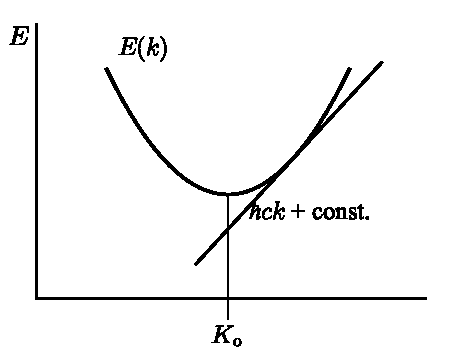
\includegraphics[width=0.72\textwidth]{fig_35.pdf}
\caption*{图 35}
\end{figure}

我们立刻意识到，这迫使我们修改准粒子元激发的原始定义，因为在这种情形下，准粒子态不再是
整个系统的严格本征态。这是一种普遍现象：在几乎所有的情形中，由于总存在这种或那种散射的
可能性，元激发态都不是完全严格的本征态。

就我所知，还从未有人在有散射存在时给出过准粒子的绝对严格的数学定义；但定义准粒子的方式
有若干种，在任何一个给定的情形中它们都可以是令人满意的。这些方式可以归入两条思想路线，
我们分别称之为"赝哈密顿量"（pseudo-hamiltonian）方法和"完全重整化"（full
renormalization）方法。

这两条处理问题的一般思想路线中的第一条，本质上就是我们在讨论形变势时已经实行过的那套
做法。也就是说，我们尽最大努力把准粒子与晶格运动彼此完全独立地定义出来，并把它们的相互
作用显式地留在问题之中。在形变势的讨论中，我们实际上是走进固体内部，给所有离子实装上刚性
夹钳，把它们绝对固定在与某种长波长晶格形变相应的位置上。由此我们得到准粒子能量对形变的
某种依赖关系，而当我们松开夹钳时，它就充当了电子-声子相互作用能。用形式化的语言说，我们
为准粒子建立了一个有效哈密顿量

\begin{equation*}
\mathcal{H}_{\text{eff}} \;=\; \int \mathrm{d}r \int \mathrm{d}r'\;\, q^{\dagger}(r)\, H_{\text{eff}}(r,r')\, q(r')
\end{equation*}

其中 $H_{\text{eff}}(r,r')$ 是局域形变 $\Delta(r)$ 和 $S(r)$ 的线性函数。于是我们可以把
$\Delta(r)$ 和 $S(r)$ 本身作为多体问题的量子化坐标引入，它们将带来一个必须添入的、二次型
的自能 $\sum_{k}\hbar\omega_{\mathbf{K}}^{0}\,(P_{\mathbf{K}}^{2} + Q_{\mathbf{K}}^{2})$。
我们希望，相互作用项随后可以由微扰论计入，并导致准粒子的散射，如下：散射哈密顿量就是
形变势，即式 (9)：

\begin{equation*}
\mathcal{H}' \;=\; E_{\Delta} \sum_{k\mathbf{K}} \Delta(\mathbf{K})\;\, q_{k+\mathbf{K}}^{\dagger} q_{k}
\end{equation*}

$\Delta(\mathbf{K})$ 与声子产生算符 $b_{\mathbf{K}}^{*}$ 之间关系的归一化，可以由能量
表达式得到：

\begin{equation*}
\frac{S}{2}\,\bigl|\Delta\bigr|^{2} \;=\; \text{势能} \;=\; \frac{1}{2}\,(\text{总能量}) \;=\; \frac{1}{2}\,\hbar\omega_{\mathbf{K}}\Bigl(n_{\mathbf{K}} + \frac{1}{2}\Bigr)
\end{equation*}

其中 $S$ 是压缩刚度 $\rho c^{2}$，而 $\omega_{\mathbf{K}} = c\mathbf{K}$ 是声子的频率。
于是我们可以取

\begin{equation*}
\Delta(\mathbf{K}) \;=\; \frac{1}{2}\sqrt{\frac{\hbar\mathbf{K}}{\rho c}}\;\bigl(b_{\mathbf{K}}^{*} + b_{-\mathbf{K}}\bigr)
\end{equation*}

由含时微扰论给出的、从单一态进入一个态连续统的逆平均自由时间（即跃迁速率）的表达式——
也就是从 $k$ 进入已自发发射了一个声子 $\mathbf{K}$ 的那些态的速率——是

\begin{equation*}
\frac{\hbar}{\tau} \;=\; 2\pi\,\bigl|\text{M.E.}\bigr|^{2}\,\frac{\mathrm{d}n}{\mathrm{d}E}
\end{equation*}

当然，M.E. 指的是散射矩阵元。物理上唯一有趣的情形，是电子动量相当大的情形，此时

\begin{equation*}
\frac{\hbar^{2}k^{2}}{2m} \;\gg\; \hbar k c\,,\qquad k \;\gg\; K_{0} = \frac{mc}{\hbar}
\end{equation*}

在这种情形下，声子造成的动量变化远大于能量变化，于是 $|k+\mathbf{K}| \cong |k|$
（图 36）。这时 $\mathrm{d}n/\mathrm{d}E$ 就恰好是电子谱中的态密度（density of states）。

\begin{figure}[H]
\centering
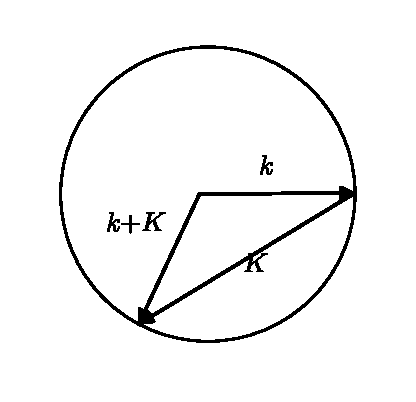
\includegraphics[width=0.72\textwidth]{fig_36.pdf}
\caption*{图 36}
\end{figure}

散射前的寿命如何计算，我留作练习：结果是

\begin{equation*}
\frac{\hbar}{\tau} \;=\; \frac{4\pi^{2}}{3}\, E^{2} \left(\frac{m^{2}}{\hbar^{3}\rho c}\right) \left(\frac{\hbar^{2}k^{2}}{2m}\right)
\tag{10}
\end{equation*}

若晶格常数为 $a$，则 $\rho \cong M/a^{3}$，而 $\hbar^{2}/ma^{2}$ 与电子能量 $\sim 1$ Ry
同量级；$\hbar c/a$ 与 $\sqrt{m/M} \times 1$ Ry 同量级。形变势常数 $E$ 同样可以预期为
1 Ry 的量级，因为百分之百的形变必然会使电子的能量完全改变；于是我们可以说

\begin{equation*}
\left.\frac{\hbar}{\tau}\;\right|_{\;\left(E_{k} \,=\, \frac{\hbar^{2}k^{2}}{2m}\right)} \;\sim\; \sqrt{\frac{m}{M}}
\end{equation*}

我们看到 $\hbar/\tau$ 确实非常小，而且对能量最低的准粒子令人满意地趋于零。

与散射相伴随的，是在等能面附近有一些态被混杂进来：对给定的能量差 $\Delta E$，微扰论给出
这部分混杂为

\begin{equation*}
\frac{\bigl|\text{M.E.}\bigr|^{2}}{(\Delta E)^{2}}\;\,\mathrm{d}n
\end{equation*}

于是，在能量上离开准粒子态超过 $\Delta E$ 的那些态的总混杂为

\begin{equation*}
\bigl|\text{M.E.}\bigr|^{2} \int_{\Delta E}^{\infty} \frac{\mathrm{d}n}{\mathrm{d}E}\,\frac{\mathrm{d}E}{E^{2}} \;\cong\; \frac{\hbar}{\tau}\,\frac{1}{\Delta E}
\end{equation*}

显然，如果允许任意低能量的态混入，此式就会发散。这意味着，任何想在有散射存在时把准粒子
态定义为严格本征态的尝试都注定失败。正如我所强调过的，我们可以沿两条途径处理这个问题：
第一条就是我们刚才描述的有效哈密顿量理论，其中准粒子是一个"被夹住的"（clamped）系统的
严格本征态，而电子-声子相互作用保留在总哈密顿量之中，我们试图用这个总哈密顿量去求解任何
输运问题等等。

与之相对的第二种方法，是试图把系统当作一个整体来处理，并定义由于散射而随时间衰变的准粒子
态。这是现代多体理论家更青睐的方法；见 Nozières (68)。正如我们稍后将要讨论的，这样的
准粒子态不仅带有重整化常数 $Z$，还带有复能量 $E_{k} + i(\hbar/\tau)$；我们说它们是
"格林函数（Green's function）的复极点"。它们与完全重整化理论的传播子（propagator）
相联系；有效的电子-声子相互作用可以作为理论的重整化顶角（vertex）部分引入，等等。要在
这种完全重整化的形式下开展整个输运理论等等，目前还差不多只是一个纲领，但毫无疑问它完全是
可行的。在半导体和绝缘体中，第一种方法迄今为止肯定是足够的，而且它免去了随身携带诸如 $Z$
这类各种非物理重整化参数的必要。

尽管如此，也有人可以争辩说第一种方法有点含糊而且不合乎物理，因为真实的准粒子随身携带着
一大片声子极化云，尤其是短波长声子和光学声子的极化云。但我们可以设想，只对那些真正能使
准粒子受到散射的长波长声子加上夹钳；这几乎不会影响准粒子的极化云，却使我们能够相当严格地
定义它们。特别是，准粒子既然与 $N+1$ 体系统的严格本征态相关联，就具有固定的动量并携带
电荷 $e$，只是处理 $Q\to 0$ 极限时须加小心——这一点我们已经讨论过了。在存在场时，它们将
服从通常类型的输运方程，带有通常的 Lorentz 力。

这种处理绝缘体中准粒子问题的方法看起来是完全严格而准确的，至少对非压电晶体和足够低的
温度是如此。然而，在电子-声子耦合极强的某些情形中，伴随电子行进的极化云的效应可能相当大。
这在某些 d 带氧化物晶体中是典型的：给定离子上 d 壳层能级中的一个电子可以使周围的离子发生
相当严重的极化，其幅度相对于这些离子的零点涨落而言相当可观。电子跳跃到另一个 d 壳层离子
上去的矩阵元的幅度可以写成

\begin{align*}
b_{d_{1}d_{2}} &= \bigl(\Psi_{d_{1}}\,|\,\mathcal{H}\,|\,\Psi_{d_{2}}\bigr) \\
&\cong \bigl(a_{d_{1}}\,|\,\mathcal{H}_{\text{el}}\,|\,a_{d_{2}}\bigr) \bigl(\Psi_{\text{lattice}}(\text{电子在 } d_{1}\text{ 上})\,\big|\,\Psi_{\text{lattice}}(\text{电子在 } d_{2}\text{ 上})\bigr)
\end{align*}

$a$ 是 d 带的普通 Wannier 函数，而 $\Psi_{d}$ 是完整的多体波函数。第二个因子——晶格
波函数的交叠——将会很小，这就大大增加了准粒子的有效质量。这就是与"自陷极化子"相对应的
物理图像——它能够运动，但只能带着大为减小的矩阵元和大为增大的 $m^{*}$ 运动。甚至在相当
低的温度下，电子通过热激活而不是通过这种隧穿过程来运动的概率也可能变得很大，这意味着这类
材料中的输运根本不像普通半导体中的输运（文献 (71)）。

在更高温度下，即使在正常情形中，热激发声子造成的额外散射也会变得远大于发射所致的自发
散射。声子寿命中的（矩阵元）$^{2}$ 因子必须再乘上一个占据因子：发射时为 $n+1$，吸收时为
$n$，其中 $n = 1/[\exp(\hbar\omega/k_{\mathrm{B}}T) - 1]$。对半导体中那些有关的声子——
即满足

\begin{equation*}
\mathbf{K}_{\text{phonon}} \;\sim\; k_{\text{electron}}
\end{equation*}

的声子——这个因子可以变得相当大，其中

\begin{equation*}
k_{\text{electron}} \;=\; \frac{\sqrt{2m^{*}k_{\mathrm{B}}T}}{\hbar}
\end{equation*}

\begin{equation*}
n(\mathbf{K}) \;\sim\; \frac{k_{\mathrm{B}}T}{\hbar c\mathbf{K}} \;=\; \frac{V_{\text{el}}}{c} \;\sim\; 10 \qquad \text{（在 } 50{-}100\,^{\circ}\mathrm{K}\text{ 时）}
\end{equation*}

最慢的那些电子所受的热散射可以变得极端严重，即使在低温下也是如此，尽管这在物理上似乎并不
十分重要。在更高温度下，我们的散射率 $\hbar/\tau$ 公式 (10) 要乘以 $k_{\mathrm{B}}T/\hbar c\mathbf{K}$
（译注：原书此处印作 $k_{0}T$，按上下文应为 $k_{\mathrm{B}}T$），并且由于 $\mathbf{K}$
与 $k$ 同量级、$k_{\mathrm{B}}T$ 按 $k^{2}$ 变化，我们得到

\begin{equation*}
\frac{\hbar}{\tau} \;\sim\; \frac{E^{2}}{\rho c^{2}}\, k^{3} \;\sim\; T^{3/2}
\end{equation*}

迁移率 $\mu = e\tau/m$ 的 $T^{-3/2}$ 依赖关系是半导体中众所周知的结果。注意，随着 $T$
增大，$\hbar/\tau$ 将相当快地变得比 $k_{\mathrm{B}}T$ 还大。

我不知道有任何关于这种情形的讨论；在其中，若没有进一步的论证，准粒子概念是不应使用的。
它出现在室温下迁移率为 10 左右的区域——在劣质半导体中这是并不罕见的一类数值。

金属中电子-声子散射变强时的效应，比起绝缘体和半导体中的情形来，被人们理解得少得多。
金属中在低温下，费米面（Fermi surface）附近的电子不能发生自发发射，因为末态电子态已被
占满。导致电子散射寿命的热吸收与热发射过程有两种不同的温度依赖关系。低温下只有长波长声子
被激发。各位当会记得，散射矩阵元正比于 $\mathbf{K}^{1/2}$，而可能的末态近似地位于
$\mathbf{K}$ 空间中的一个球面上，其面元 $\propto \mathbf{K}\,\mathrm{d}\mathbf{K}$。于是

\begin{equation*}
\frac{\hbar}{\tau} \;\propto\; \int_{0}^{\mathbf{K}_{F}} \frac{\mathbf{K}^{2}\,\mathrm{d}\mathbf{K}}{\exp(\hbar c\mathbf{K}/k_{\mathrm{B}}T) - 1} \;\propto\; \left(\frac{k_{\mathrm{B}}T}{\hbar c}\right)^{3}
\end{equation*}

在高于 Debye 温度的温度下，所有声子态的占据数都正比于 $T$，而
$\hbar/\tau \propto T/\theta_{D}$（图 37）。

我们可以在高温极限下区分两种情形：$\hbar/\tau$ 大于或小于 $kT$。当 $\hbar/\tau < kT$
时，无论哪一类微扰论大概都会相当令人满意，

\begin{figure}[H]
\centering
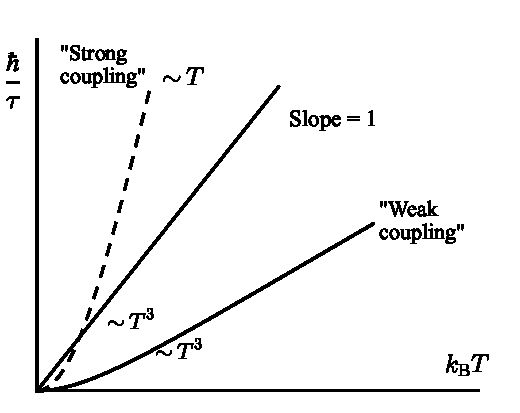
\includegraphics[width=0.72\textwidth]{fig_37.pdf}
\caption*{图 37}
\end{figure}

\section{金属中的准粒子：费米液体}

Landau 的“费米液体”（Fermi liquid）理论（73）或许可以被看作“钳位”（clamping）或有效哈密顿量观念的一种问题多得多的应用。Landau 理论试图把准粒子观念应用于相互作用很强的简并费米气体（degenerate Fermi gas），例如金属中的电子，或低温下的液体 He$_3$。

在这里，散射是电子自身之间相互作用的效应，因此若要完全以钳位理论来论证准粒子的使用，就意味着不仅要对离子实的运动加钳位，还要对电子气体本身加钳位。但这件事无法以任何十分严格的方式做到。

Landau 的做法是这样来施加他的“钳位”的：规定准粒子的分布 $n(k,r)$ 应当如何作为金属中位置的函数。然后，正如我们对声子存在下的准粒子所做的那样，他假定一个给定的波包 $q_k^{\dagger}(r)$，其能量随同一区域内其他准粒子的密度而变化：

\begin{equation*}
E_k(r) \;=\; E_k^{0} \;+\; \sum_{k'} f_{kk'}\, n(k', r)
\end{equation*}

有必要保留指标 $k$，用以指明准粒子波包以哪个 $k$ 值为中心，因为低能的准粒子在动量空间中可以铺展到整个费米面。因此我们必须谨慎地处理分布函数 $n$，因为 $k$ 和 $r$ 不是对易的变量，只能粗略地加以指定。

我们至今还没有说明准粒子波包究竟是什么的波包。在这里，即便是系统最低的精确激发态也极其复杂。这一点可以直接从最低阶微扰论看出来。考虑一个粒子 $k$，它已被激发到费米面之上到达 $k_F+a$，这构成无相互作用 Fermi 系统最简单的激发态之一。这一电子可能被散射 $k = k_F + a \to k - q$，此过程同时把第二个电子 $k'$ 激发到 $k'+q$；只要末态中所有的能量都高于费米能，该过程就不为 Pauli 原理所禁止
\begin{figure}[H]
\centering
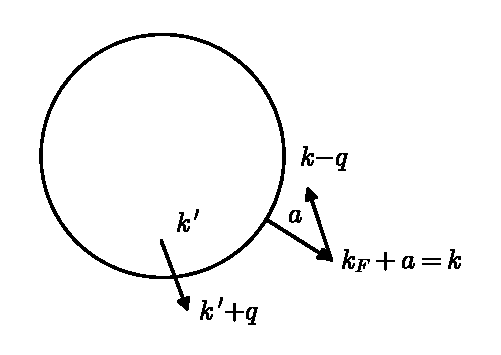
\includegraphics[width=0.72\textwidth]{fig_38.pdf}
\caption*{图 38}
\end{figure}
（图 38）。毫无疑问各位早已熟知，由此得到的平均自由时间按能量增量的平方变化，

\begin{equation*}
\Delta E \;=\; \frac{\hbar^{2}}{2m}\left[(k_F+a)^{2} - k_F^{2}\right] \;\simeq\; \frac{\hbar^{2}}{m}\, k_F a
\end{equation*}

\begin{equation*}
\frac{\hbar}{\tau} \;=\; \text{consts.} \times \frac{|V|^{2}\,(\Delta E)^{2}}{E_F^{3}}
\end{equation*}

这一点很容易看出，只要注意到：对任何一个空穴留在 $k'$ 态的末态，能量守恒要求

\begin{equation*}
k^{2} - (k-q)^{2} \;=\; (k'+q)^{2} - k'^{2}
\end{equation*}

或

\begin{equation*}
(k - k') \cdot q \;=\; q^{2}
\end{equation*}

这是以 $(k-k')$ 为直径的球面的方程：于是我们知道，$k'+q$ 必定落在以从 $k$ 到 $k'$ 的矢量为直径的球面上。当 $a$ 很小时，这个球面可以用通过 $k$ 和 $k'$ 的平面来近似，因为 $k'$、$k$、$k-q$ 和 $k'+q$ 都必须非常靠近费米面（除了 $k' \simeq -k$ 的情形，而这只占可用态中极小的一部分）。现在很清楚，若 $k'$ 位于费米面以内 $(a\cos\theta)$ 的深度处，则可能存在两类散射过程：若我们选取一个垂直于 $(k-k')$ 且较小的 $q$（$q > |k_F - k'|\cos\theta$，$q < a\cos\theta$），便可以有 $k \to k-q$、$k' \to k'+q$，或者 $k \to k'+q$、$k' \to k-q$（图 39）。无论哪种情形，对给定的 $\theta$，$k'$ 与 $q$ 的可能范围都与 $a$ 成正比，而 $a \propto \Delta E$；于是在这个 $\theta$ 处的总散射概率 $\propto (\Delta E)^{2}$。对 $\theta$ 作积分、从而得到具有给定 $\Delta E$ 的电子的 $\hbar/\tau$ 的完整表达式，这个问题我留作练习。

\begin{figure}[H]
\centering
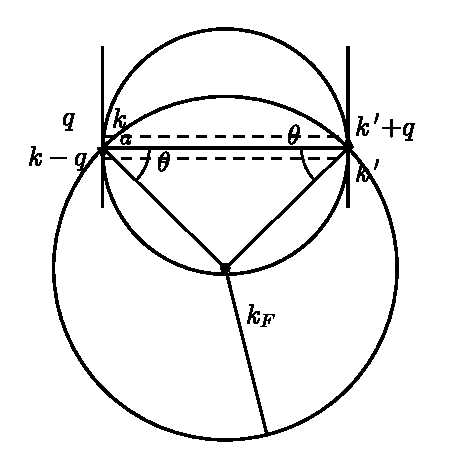
\includegraphics[width=0.66\textwidth]{fig_39.pdf}
\caption*{图 39}
\end{figure}

使人有理由相信，即便存在散射准粒子概念仍有某种意义的，是这样一个事实：至少在最低阶上，电子的寿命在其能量趋近费米面时非常迅速地变长。如果我们考察更高阶的散射，就会发现不相容原理把它们削减得比我刚才讨论的最低阶效应还要彻底得多。Goldstone、Luttinger、Ward 以及其他若干作者（74）从普遍的场论式、完全重整化（full-renormalization）的进路处理过这个问题。也就是说，他们证明了：通过对微扰论所有阶求和，人们可以如何从无相互作用气体的谱、态密度、以及——把二者一并概括起来的——Green 函数，绝热地延拓到有相互作用气体的相应量。

在绝缘体的情形，各位当还记得，我们把系统的 Green 函数写成

\begin{equation*}
G(k, t) \;=\; \langle g|\, c_k^{\dagger}(t)\, c_k(0)\, |g\rangle
\;=\; Z\, e^{iE_k t} \;+\; \int \mathrm{d}E_n\, f(E_n)\, e^{iE_n t}
\end{equation*}

系统的能谱也可以用以频率表出的 Green 函数来定义：

\begin{align*}
G(k, \omega) \;&=\; i \int G(k, t)\, e^{-i\omega t}\, \mathrm{d}t \\
&=\; \frac{Z}{\omega - E_k} \;+\; \int \frac{f(E)}{\omega - E}\, \mathrm{d}E
\end{align*}

通过 $c_k^{\dagger}$ 产生的那些态的实际能谱，与 $\mathrm{Im}\, G(k)$ 相联系；准粒子态的存在，由 $G$ 在 $E_k$ 处出现一个极点来标志。多体理论所做的，就是证明：至少到微扰论的所有阶，\emph{在金属中}假定 $G$ 在一个复能量

\begin{equation*}
E_k \;+\; i\,\frac{\hbar}{\tau}
\end{equation*}

处有极点是自洽的，于是 $i\hbar/\tau$ 就是能量的虚部，也就是相应谱的宽度。事实证明，这一宽度按 $(\Delta E_k)^{2}$ 趋于零，恰好足以允许一个锐利费米面的存在，因为当准粒子态趋近费米面时，它们的定义便随之变得精确。在金属中，作为时间函数的 Green 函数起初迅速下降，一如它在绝缘体中的表现，然后以频率 $E_k/\hbar$ 振荡；但振荡不再无限延续，而是以 $1/\tau$ 的速率被阻尼（图 40）。

\begin{figure}[H]
\centering
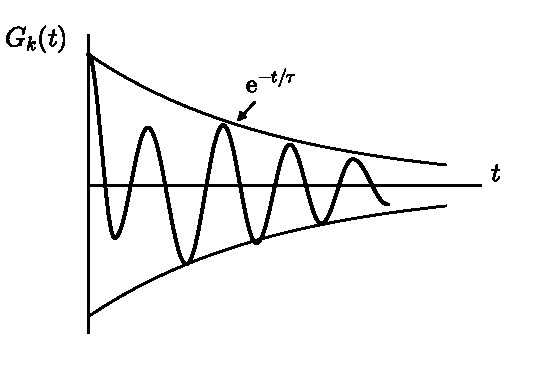
\includegraphics[width=0.72\textwidth]{fig_40.pdf}
\caption*{图 40}
\end{figure}

\begin{figure}[H]
\centering
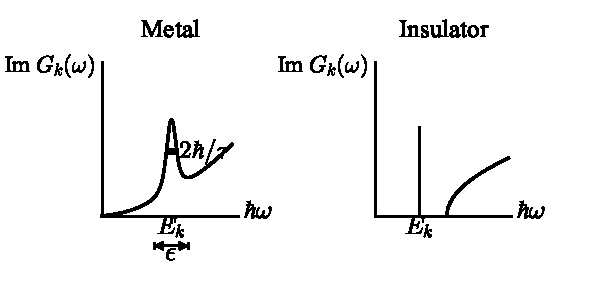
\includegraphics[width=0.72\textwidth]{fig_41.pdf}
\caption*{图 41}
\end{figure}

相应的谱密度如图 41 所示。同样，正如在绝缘体中那样，我们可以对态 $c_k^{\dagger}\Psi_{g}$ 施加一个能量滤波器，从而由它重构出准粒子态：

\begin{equation*}
q_k^{\dagger}\,\Psi_{g} \;\propto\; \int_{E_k-\frac{\epsilon}{2}}^{E_k+\frac{\epsilon}{2}} c_k^{\dagger}\,\Psi_{g}(E)\,\mathrm{d}E
\qquad \epsilon \;\geq\; \frac{\hbar}{\tau}
\end{equation*}

当然，形式上这很容易写成一个时间积分：

\begin{equation*}
q_k^{\dagger}\,\Psi_{g} \;=\; \int_{0}^{\infty} \mathrm{d}t\;\, e^{\left(i\frac{E_k}{\hbar} \,-\, \frac{\epsilon}{2\hbar}\right)t}\; c_k^{\dagger}(t)\,\Psi_{g}
\end{equation*}

当 $E_k \to 0$ 时，量 $\epsilon$ 可以取得比 $E_k$ 更快地趋于零；这正是我们能够定义一个锐利的费米面、并给某一给定的准粒子态指派一个确定占据概率的原因。

准粒子图像的限度显然是 $\hbar/\tau < E_k \sim k_B T$，而且 \emph{a fortiori}（更不必说）$\hbar/\tau < E_F$；$\hbar/E_F$ 是 $G(t)$ 初始下降的时间常数。

从这一类理论出发，并借助用图形方法证明的各种恒等式，Luttinger 和 Nozières 最近直接从微扰论得到了 Landau 费米液体理论的许多结果（75）。显然，目前还不可能把这种“完全重整化”型的理论重新表述成“有效哈密顿量”或钳位理论。由于“有效哈密顿量”做法更为方便，尤其是对输运问题，这是相对 Landau 直观进路的一个不利之处。此外，微扰论的做法必须假定收敛性，而“微扰论（P.T.）从不收敛”几乎是一句格言；并且可以证明，这一个理论恰恰不收敛。

一个值得提出的好问题是：某种更直截了当的“钳位”式进路是否就不能用于这个问题。我们可以问：正如声子理论中的情形那样，我们能否在不严重改变准粒子性质的前提下，把 $N$ 粒子系统那些必要的自由度钳制住。做到这一点的一种办法，也许是对 $N$ 粒子系统强加一个要求：不允许激发长波长的自由度——也就是说，要求密度涨落

\begin{equation*}
\rho^{Q} \;=\; \sum_{k} c_{k+q}^{\dagger}\, c_{k}
\end{equation*}

或者甚至个别的这类密度涨落

\begin{equation*}
\sum_{\substack{\text{some small}\\ \text{region of } k}} c_{k+q}^{\dagger}\, c_{k}
\end{equation*}

对某个足够小的 $q$ 恒等于零。由于在 $N+1$ 粒子问题中我们可以假定，就长程效应而言准粒子密度与真实粒子密度是相同的（当然仍需附带关于 $q=0$ 极限的那些非常特殊的评注），这将等价于把 Landau 的 $n(k,r)$ 固定下来。

遗憾的是，显然即便如此，也仍不能使准粒子成为系统的精确激发，原因是存在我们曾提到过的“交换”散射过程 $k \to k'+q$、$k' \to k-q$——每一个长波过程都各配有一个这样的过程——此外，还有 $k' \simeq -k$ 那个有趣的区域，在那里所有的 $q$ 都是允许的。也许能找到绕开交换散射问题的某种办法；但耐人寻味的是，微扰论已知的种种失效恰恰与 $k' \simeq -k$ 区域相联系（76）。

令人失望的是，准粒子观念以及费米气体的有效相互作用的完整论证至今尚未出现。由于这些概念在 Landau 准经典分布函数并不是令人满意的进路的那些场合被大量使用——尤其是超导电性和强杂质散射的情形——拥有一个更充分的论证将是极为可取的。

在结束时，我想说：准粒子观念对固体物理是一个无比重要的观念，当然对高能物理也是如此。关于准粒子，各种严格的或或多或少严格的思考方式，给了我们十分宝贵的信心：对物理思维的种种基础。尽管如此，人们也可能过分强调处理固体时所能达到的、乃至宜于讲求的那种严格性。正如 Landau 在旧版《Statistical Physics》的序言中所说：“我们在这里谈的是理论物理，因此数学上的严格性当然是既不相干、也办不到的。”这话并不完全正确，但也相去不远。

我们最好记住：第一，我们用来工作的数学模型，几乎总是对实际物理系统已经作了高度简化的理想化；第二，准粒子物理就其本性而言全部建立在微扰级数之上，因为它无非是试图用一个形如仅有弱相互作用粒子系统的理论去逼近一个完整的理论。但我们必须时时猜测微扰论应当从什么状态出发——也就是说，猜测系统的物理本性究竟是什么：金属型的、磁性的、绝缘的、液态的还是固态的。这种猜测可能正确，但也可能错得离谱；在后一种情形，往往唯一的迹象只是我们的微扰论出现轻微的、几乎觉察不到的发散。超导电性里发生的正是这种事。第三点警告是：由于存在集体激发，几乎所有微扰级数都确实会在至少某个方面失效，而这些集体激发又往往只能作为各项发散子级数之和从微扰论中求得。总的说来，我认为下述态度至少是站得住脚的：固体物理的奠基者们和 Landau 学派对准粒子的本能式使用，其严格性比起精巧的多体理论几乎毫不逊色，而且也许更万无一失，因为它的\emph{外表}不那么严格。

\section{集体激发}

\subsection{激子}

绝缘体中的激子（exciton）与铁磁体中的自旋波（spin wave）是最简单的两类集体激发（collective excitation）。它们在许多方面惊人地相似，在与它们相联系的形式数学方面尤其如此；两者还有更深一层的相似之处：它们的零点运动（zero-point motion）都相对很少，由零点运动所带来的复杂问题也很少。在每一种情形下，原因都在于：正如在 $N+1$ 体问题中那样，人们可以从一个几乎能够严格定义的基态出发来表述问题。在铁磁体中之所以如此，是因为铁磁基态的特征（如果它存在的话）是自旋的总 $Z$ 分量为 $M_Z = N/2$。所有自旋波态虽然能量可能非常低，其特征却是 $M_Z = (N/2) - 1$，因而把它们与基态联系起来的哈密顿量矩阵元充其量也非常小。

激子的情形则更为复杂。如读者所知，激子是光激发，我们既可以按照 Frenkel (77) 的模型、也可以按照 Wannier (78) 的模型来讨论它们。Frenkel 模型适用于紧束缚的情形，例如分子型或离子型晶体，它由一个在晶体中移动的受激原子态构成。例如，它可以是这样一种 NaCl 中的态：Na$^+$ 离子实的 p 电子之一被激发到一个 s 能级，而由此形成的激发可以在晶体中移动。Wannier 模型更常被观察到，或许也更有趣；在这一模型中，人们假定一个电子从一个能带被激发到下一个能带，但由此形成的准粒子与准空穴按弱势 $e^2/\kappa R$ 相互吸引，并一起在晶体中穿行。无论哪种情形，通常都相当清楚该如何定义一个不包含任何激子的固定基态；例如，对光学活性的（optically active）激子——诸如 $sp$ 跃迁——$k=0$ 的激子态与基态宇称相反，因而不能与基态混合。然而我们将会看到，这一简化并非对所有激子都完全成立。

我这里的材料将主要取自 J.~J.~Hopfield (79) 的一篇出色的论文，以及 E.~Dresselhaus (80) 的另一篇。我不认为存在任何好的综述；较早的理论在 Seitz 的书中有论述。

就定性物理图象的目的以及与自旋波作比较而言，Frenkel 模型更为有用。让我们从它出发，然后再从它出发作微扰。

Frenkel 模型（至少在一开始）所设想的是一种像固态 Ne 或 Ar 那样的晶体，其中的原子相距相当远，几乎互不交叠。当然，这种晶体是一种绝缘体。我们暂且撇开对基本多体问题的任何讨论，而用 Hartree-Fock 方法处理势场；相关的相互作用我们稍后将用多体理论来处理，但从 Hartree 出发最为简单，同时按惯例附加上一个条件：由于我们处理的是元激发，多体效应并不太严重。最后一个被填满的能带，我们假定是一个 s 带。把这个带的 Wannier 函数记作 $a_s(r-R_j)$。由于这个带极窄，非对角矩阵元
\begin{equation*}
b_{jk}^{s} \;=\; \int a_s^{*}(R_j - r)\; \mathcal{H}_{1\mathrm{el}}(r)\; a_s(r - R_k)\; dr
\end{equation*}
非常小——至于相对于什么而言小，我们很快就会看到。

还有一个“导”带——一个由激发态构成的能带，为简单起见我们同样假定它具有 p 型 Wannier 函数
\begin{equation*}
a_p^{\,x,y,z}(r - R_j)
\end{equation*}
以及非常窄的带宽（即转移积分，transfer integrals）
\begin{equation*}
b_{jk}^{xx'},\ \text{等等}
\end{equation*}
自由原子会有一定的激发能
\begin{equation*}
E_0 \;=\; (E_p - E_s)
\end{equation*}
——从 s 态激发到 p 态——在这样一种固体中，它不会由于变换到 Wannier 函数而受到太严重的修正。必须认识到，这个激发能在数量上并不接近 s 带与 p 带之间的 Hartree-Fock 平均能量差。

其原因在于：能带能量差对应的态，是电子被完全激发而离开自己原来那个原子、从而发现自己处在一个既有 s 又有 p 电子的原子上的态，因此除了单电子激发能 $E_0$（图 42）之外，还有如下的额外库仑排斥能
\begin{equation*}
U \;=\; \int |a_p(r-R_j)|^2\; \frac{e^2}{|r-r'|}\; |a_s(r'-R_j)|^2\; dr\; dr'
\end{equation*}

\begin{figure}[H]
\centering
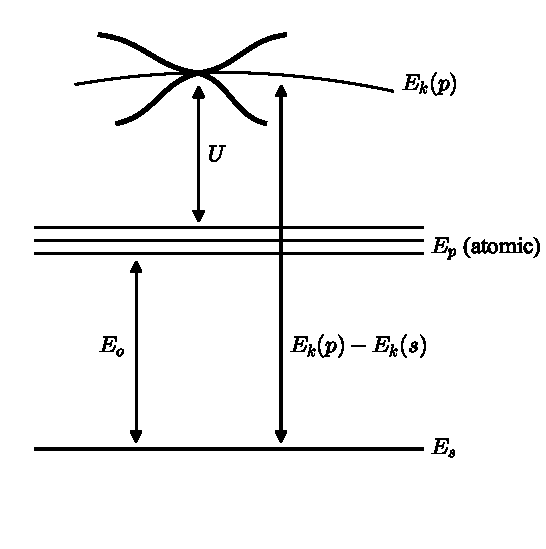
\includegraphics[width=0.72\textwidth]{fig_42.pdf}
\caption*{图 42（能级示意图：上方为 $E_k(p)$ 能带曲线，下方为 $E_p$(atomic) 原子能级线组与 $E_S$ 基态能级线；竖直箭头分别标出 $E_0$、$E_k(p)-E_k(s)$ 两个激发能以及 $U$ 的间隔）}
\end{figure}

换一种说法：电子与它身后留下的空穴通过完全的库仑相互作用（仅被介质的介电常数稍微修正）彼此强烈吸引，因此电子被激发到同一原子上的 p 态，远比把它激发到邻近的原子上去容易得多。

现在很清楚，如果各个 $b$ 与 $U$ 相比很小，那么 Frenkel 理论将相当好地成立，因为无论空穴还是电子都不会倾向于跳离自己的同伴。这时激子
\begin{figure}[H]
\centering
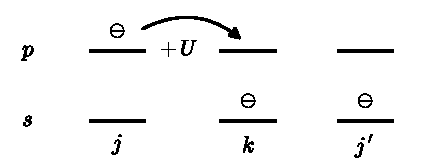
\includegraphics[width=0.72\textwidth]{fig_exciton-jkj.pdf}
\caption*{无编号正文插图（原书不编号）——Frenkel 激子组态示意：上排为 p 能级，格点 j 处有一个电子（$\ominus$），一道弧形箭头从该电子指向右侧格点 k 处的空 p 能级，箭头旁标 “+ U”；下排为 s 能级，格点 j 处为空穴，k 与 j' 处各有一个电子（$\ominus$）}
\end{figure}
将是紧束缚的，而且在 s 空穴-p 电子带态的连续谱与激子之间将有一个很大的能隙。在另一种情形 $U < b$ 中，电子与空穴将比较容易分开，Wannier 图象会好得多。我们将在后面讨论那种情形。

另一方面，即使电子与空穴耦合得很紧，这一对粒子仍然能够一起在晶体中移动。在我们现在的情形中，实现这一点最重要的机制，是电子与相邻原子上的电子之间的相互作用。这个相互作用可以写成
\begin{equation*}
\int \psi^{\dagger}(r)\,\psi^{\dagger}(r')\,\frac{e^2}{|r-r'|}\,\psi(r')\,\psi(r)\,dr\,dr' \tag{11}
\end{equation*}
其中 $\psi$ 可以用 Wannier 函数的产生与湮灭算符展开，即 $c_j^s$ 与 $c_j^{p_x}$、$c_j^{p_y}$、$c_j^{p_z}$：
\begin{equation*}
\psi^{\dagger}(r) \;=\; \sum_j \sum_{n=s,\,p_x,\,p_y,\,p_z} c_j^{n\dagger}\, a_n^{*}(r-R_j)
\end{equation*}
有各种各样的项可能产生把一个原子激发、同时使其邻居退激发的效果；其中最重要的是“直接的”（direct）即偶极（dipolar）项，其典型的一员是
\begin{equation*}
\left(c_j^{p_x}\right)^{\dagger} c_k^{s\dagger} c_k^{p_x} c_j^{s} \int a_{p_x}^{*}(r-R_j)\, a_s(r-R_j)\, \frac{e^2}{|r-r'|}\, a_s^{*}(r'-R_k)\, a_{p_x}(r'-R_k)\, dr\, dr'
\end{equation*}
这类积分用多极展开（multipolar expansion）来求值最为容易：
\begin{align*}
\frac{e^2}{|r-r'|} = \; & e^2 \Bigg[ \frac{1}{R_j - R_k} + \left\{ (r-R_j) + (r'-R_k) \right\} \cdot \nabla\!\left(\frac{1}{r}\right)\Big|_{R_j-R_k} \\
& + (r-R_j)(r-R_k) \cdot \nabla\nabla\!\left(\frac{1}{r}\right)\Big|_{R_j-R_k} + \cdots \Bigg] \tag{12}
\end{align*}

（译注：式 (12) 照录原书。按标准多极展开，第二项花括号内应为 $\{(r-R_j)-(r'-R_k)\}$，即 $(r'-R_k)$ 之前应为负号；原书印作正号。）

第一个不为零的项是偶极项，即上式最后一项，它给出的典型矩阵元为
\begin{equation*}
|X_{sp}|^2 \cdot T(r_j - R_k)_{xx}
\end{equation*}
其中 $X_{sp}$ 是原子态的偶极矩矩阵元：
\begin{equation*}
X_{sp} \;=\; e \int a_{p_x}^{*}(r)\; x\; a_s(r)\; dr
\end{equation*}
而 $T$ 是偶极相互作用算符
\begin{equation*}
T_{jk} \;=\; \frac{1}{R_{jk}^{3}} \left\{ 1 - 3\,\frac{\mathbf{R}_{jk}\,\mathbf{R}_{jk}}{R_{jk}^{2}} \right\}
\end{equation*}

在这个偶极相互作用算符——它表示与每个原子相联系的运动电偶极子之间的直接静电相互作用——之中，我上面给出的那种形式的矩阵元所联系的各个态，正如我先前概略说明的那样，每一个都比基态高出大约 $E_0$ 的能量。还有一些形如 $c_j^{p\dagger} c_j^{s} c_k^{p\dagger} c_k^{s}$ 的项，它们同时产生或湮灭两个激发；这些项有相当的重要性，我们很快就会回头来讨论它们，但就目前而言，它们显然不如其他项有效，因为它们的能量分母 $\Delta E$ 为 $2E_0$。于是我们的哈密顿量中现在有
\begin{align*}
\mathcal{H}_{\mathrm{unpert}} = \sum_{j,\,p_i} \frac{E_0}{2} & \left[ \left(c_j^{p_i}\right)^{\dagger} c_j^{p_i} - c_j^{s*} c_j^{s} \right] \\
& + \frac{1}{2} \sum_{j \neq k}\; \sum_{p_i\, p_{i'}} \Bigl( \left(c_j^{p_i}\right)^{\dagger} c_k^{s\dagger} c_k^{p_{i'}}\, c_j^{s}\; |X_{sp}|^2\; T_{jk} \Bigr)_{ii'} \tag{13}
\end{align*}

现在有用的一步，是几乎在集体激发理论的每一个问题中都要采取的一步：从费米子（fermion）算符对到玻色子（boson）的变换。这类变换中人们最熟悉的，是电子自旋算符这一特殊情形。假定代替三个 p 函数的只是唯一的一个 $\phi_p$。那么出现在哈密顿量——式 (13)——之中、与原子 $j$ 相联系的算符，将是如下三种组合
\begin{align*}
c_{j1}^{\dagger}\, c_{j1} - c_{j0}^{\dagger}\, c_{j0} \qquad & \qquad 0 = s \\
c_{j1}^{\dagger}\, c_{j0} \;\; \text{与} \;\; c_{j0}^{\dagger}\, c_{j1} \qquad & \qquad 1 = p
\end{align*}
此外，我们只对原子 $j$ 要么被激发、要么未被激发的那些态感兴趣——也就是说，对 $n_p + n_s = 1$ 的态感兴趣。

这些算符对恰好等价于一组 Pauli 自旋算符
\begin{equation*}
\sigma_{jz} \;=\; \begin{pmatrix} 1 & 0 \\ 0 & -1 \end{pmatrix}\;\begin{matrix} \mathrm{p}_{occ} \\ \mathrm{s}_{occ} \end{matrix} \qquad\quad \sigma_j^{+} \;=\; \begin{pmatrix} 0 & 1 \\ 0 & 0 \end{pmatrix} \qquad\quad \sigma_j^{-} \;=\; \begin{pmatrix} 0 & 0 \\ 1 & 0 \end{pmatrix}
\end{equation*}
——它们作用在描写第 $j$ 个原子状态的赝自旋（pseudo-spin）波函数上。

首先，属于不同原子的费米子算符对彼此对易，正如自旋算符那样；其次，在涉及单个原子的波函数的子空间内，这些自旋算符恰好具有与
\begin{equation*}
c_1^{\dagger} c_1 - c_0^{\dagger} c_0 \;(\sigma_z) \qquad\qquad c_1^{\dagger} c_0 \;(\sigma^{+}); \quad c_0^{\dagger} c_1 \;(\sigma^{-})
\end{equation*}
完全相同的代数性质。因此在那种情形下，把哈密顿量写成
\begin{equation*}
\mathcal{H} \;=\; \frac{E_0}{2} \sum_j \sigma_{jz} \;+\; \frac{1}{4} \sum_{jk} X_j\, T_{jk}\, X_k \left( \sigma_j^{+} \sigma_k^{-} + \sigma_j^{-} \sigma_k^{+} \right)
\end{equation*}
的形式将是精确无误的。在磁学情形中恰好就要用到这种对应。

从自旋算符到玻色子的变换，Dyson (81) 已经作过详尽的讨论；借助一个小技巧可以把它简化，这个技巧的出处我已经记不得了。只要两个自旋算符——或者两个费米子算符对——涉及的是不同的原子，它们就彼此对易，正如玻色子那样。但当两个自旋算符涉及同一个原子时，它们的对易关系要更接近费米型得多，而这正是建立相应的一组玻色子时的主要困难。

在激子的情形以及自旋的许多情形中，这并不是一个很严重的限制，因为出现的激发总数相当少，从而它们相遇重合的可能性可以忽略。在这样的情形下，我们或许可以猜想：按照下述显而易见的对应规则直接把旋量（spinor）认同为玻色子，就会令人满意：
\begin{equation*}
\sigma_j^{\dagger} \rightarrow b_j^{\dagger} \qquad \sigma_j \rightarrow b_j \qquad \frac{\sigma_{jz} + 1}{2} \rightarrow n_j \;=\; b_j^{\dagger} b_j \tag{14}
\end{equation*}
就最重要的那一对能级 $n_j = 0$ 与 $1$ 而言，算符组 (14) 具有完全相同的代数性质。但玻色子 $b$ 却具有与一整串额外能级 $n_j = 2,\, 3,\, \ldots$ 相联系的矩阵元。

使对应 (14) 成为精确的诀窍很简单：切断能级阶梯最底下两级与其余各级之间的联络。插入一道“势垒”（barrier），它恰好把连接 $n_j = 1$ 与 $n_j = 2$ 的矩阵元投影掉（project out），而在其他方面并不改变 $n_j = 0$ 和 $1$ 的矩阵元（图 43）。这道“势垒”就是：在所有使用 $b_j^{\dagger}$ 的地方都在其之前、在使用 $b_j$ 的地方都在其 \emph{之后} 乘以 $(1-n_j)$。也就是说，
\begin{equation*}
\sigma_j^{\dagger} = b_j^{\dagger}(1-n_j) \qquad \sigma_j = (1-n_j)\, b_j \qquad \sigma_{jz} = 2n_j - 1
\end{equation*}

\begin{figure}[H]
\centering
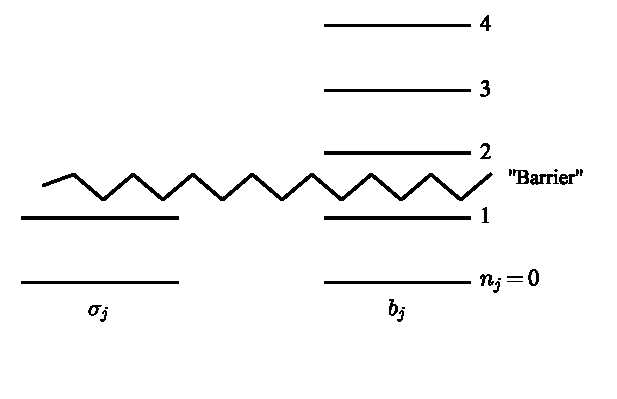
\includegraphics[width=0.72\textwidth]{fig_43.pdf}
\caption*{图 43（示意图：左边的 $\sigma_j$ 只有两个能级（0 与 1）；右边的 $b_j$ 具有包括 $n_j$ = 0、1 与 2、3、4、……在内的整个能级阶梯，在 $n_j = 1$ 与 2 之间画有锯齿状 “Barrier”（势垒））}
\end{figure}

立刻可以验证：当 $n_j = 1$ 时，$\sigma_j^{\dagger}$ 无法把它升到 $n_j = 2$，反之亦然。

别的技巧也可能同样好，例如 Holstein-Primakoff 展开或 Wentzel 的有效哈密顿量方法 (82)；某些格林函数（Green's function）方案则更为一般 (93)；但就费米子对到玻色子的变换而言，这是迄今最简单的一个论证。利用这一变换，在单激发能级的情形下，哈密顿量现在——仍然是严格地——为
\begin{equation*}
\mathcal{H} \;=\; E_0 \sum_j n_j \;+\; \sum_{jk} b_j^{\dagger}(1-n_j)\, T_{jk}\, (1-n_k)\, b_k\; \frac{|X|^2}{2}
\end{equation*}
把它推广到激发态简并的情形是平凡的。在我们正在讨论的情形中，可以把这对能级——其中之一是三重简并的——换成三维谐振子最低的两个能级
\begin{equation*}
b_j^{\dagger} \;=\; b_j^{x\dagger},\; b_j^{y\dagger},\; b_j^{z\dagger}
\end{equation*}
于是，为了施加我们的势垒，只需把 $b^x$ 乘以 $(1-n_j)$，其中 $n_j = n_{jx} + n_{jy} + n_{jz}$；这样便有 $c_j^{p_x}{}^{\dagger} c_j^{s} = b_j^{x}{}^{\dagger}(1-n_j)$，等等。所得的用玻色子表示的哈密顿量为

% （本文件到此为止；下接原书 p154，由下一文件续译）

\begin{equation*}
\mathcal{H} \;=\; E_0 \sum_j n_j \;+\; \frac{|X|^{2}}{2} \sum_{j\neq k} b_j^{\dagger}(1-n_j)\cdot T_{jk}\cdot(1-n_k)\, b_k \tag{15}
\end{equation*}

再者，(15) 是完全精确的；“动能限制”在这里已被一个非线性相互作用所取代。

从这里出发继续下去有两条途径。第二种，即直接对角化，我们稍后再来演示；第一种是直接计算玻色子算符的运动方程：

\begin{align*}
i\hbar\,\frac{db_j^{\dagger}}{dt} \;=\; \bigl[\mathcal{H},\, b_j^{\dagger}\bigr] \;=\;& E_0\, b_j^{\dagger} \;+\; |X|^{2} \sum_{k\neq j} b_k^{\dagger}\cdot T_{jk}\,(1-n_j)(1-n_k) \\
&-\; \frac{|X|^{2}}{2} \sum_{k\neq j} \Bigl[(b_j^{\dagger})^{2}\cdot T_{jk}\cdot(1-n_k)\, b_k \;+\; b_k^{\dagger}(1-n_k)\cdot T_{kj}\, n_j\Bigr]
\end{align*}

其中用到了 $[b,\, b^{\dagger}]=1$。

若让这个方程作用于没有激子被激发的基态，最后两项便恒等于零，而第二项中的那些修正项也同样为零。于是它是 $b_j$ 的一个线性方程，可以用线性变换

\begin{equation*}
b_j \;=\; \frac{1}{\sqrt{N}} \sum_k e^{i\mathbf{k}\cdot\mathbf{R}_j}\, \beta_k
\end{equation*}

把它从原子激子变换到行波来对角化。所得的方程是

\begin{equation*}
i\hbar\,\frac{d\beta_k}{dt} \;=\; E_0\, \beta_k \;+\; X^{2}\, T\cdot \beta_k
\end{equation*}

其中 $T$ 是偶极相互作用的 Fourier 变换

\begin{align*}
T_k \;&=\; \sum_{j\neq 0}\, e^{i\mathbf{k}\cdot\mathbf{R}_j}\, T_{0j} \\
&=\; \sum_{j\neq 0}\, \frac{e^{i\mathbf{k}\cdot\mathbf{R}_j}}{R_j^{3}}\, \Bigl\{\, 1 \;-\; 3\,\hat{\mathbf{R}}_{0j}\hat{\mathbf{R}}_{0j} \,\Bigr\}
\end{align*}

注意 $\sum_k T_k = 0$，因为其中不含 $j=0$ 的项。对于波长非常长的激子——也只有这类激子才真正值得注意——并且在立方晶体中或沿对称轴的方向上，$T$ 通常可以通过把纵波与横波分开而对角化；也就是说，它的一个主轴沿 $\mathbf{k}$ 方向，另外两个与之垂直。

在 $\mathbf{k}\to 0$ 的极限下，$T$ 变成著名的偶极和（dipolar sum），它在局域场理论中具有基本的重要性。当 $\mathbf{k}\to 0$ 时，

\begin{equation*}
(T_l)_k \;-\; (T_t)_k \;\to\; 4\pi N
\end{equation*}

而对立方对称的格位 $j$，

\begin{equation*}
(T_l)_k \;\to\; \frac{8\pi N}{3} \qquad\qquad (T_t)_k \;\to\; -\,\frac{4\pi N}{3}
\end{equation*}

$4\pi/3$ 正是适当的 Lorentz 局域场因子。$\mathbf{k}\to 0$ 时纵波与横波之间的差别反映了偶极力的长程性质：纵向偶极波会在波的波节与波腹处引起电荷的积累（译注：原文此处作 “modes”，据图 44 及上下文应为 “nodes”，即波节），而横波则不会（图 44）。

\begin{figure}[H]
\centering
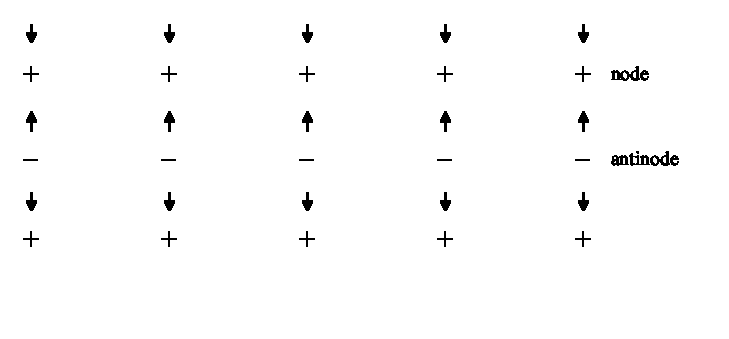
\includegraphics[width=0.72\textwidth]{fig_44.pdf}
\caption*{图 44　纵向偶极波中偶极子（箭头）与电荷（+、−）的排列：+ 电荷一行处于波节（node），− 电荷一行处于波腹（antinode）（原书图注仅作 “Figure 44”）}
\end{figure}

于是在这个近似下，激子的能量为

\begin{gather*}
E_l \;=\; E_0 \;+\; \frac{8\pi}{3}\, N X^{2} \;+\; \text{const.}\; X^{2}\, \frac{k^{2}}{a} \;+\; \cdots \\
E_t \;=\; E_0 \;-\; \frac{4\pi}{3}\, N X^{2} \;+\; \text{const.}\; X^{2}\, \frac{k^{2}}{a} \;+\; \cdots
\end{gather*}

关于偶极和，最好的处理大概要数 Cohen 与 Keffer 的一篇文章 (84)。

$T_l$ 与 $T_t$ 的实际数值依赖于结构的具体细节。但二者的差——其实也就是纵向与横向激子频率之差——即使在 Frenkel 模型并不适用的情形下也不依赖这些细节，而是一种纯粹长程的、宏观的效应。各位可以看到，$T_t$ 是由平行的偶极子产生的场之和，其中在极远距离处的表面电荷或体电荷实际上已相互抵消：

\begin{figure}[H]
\centering
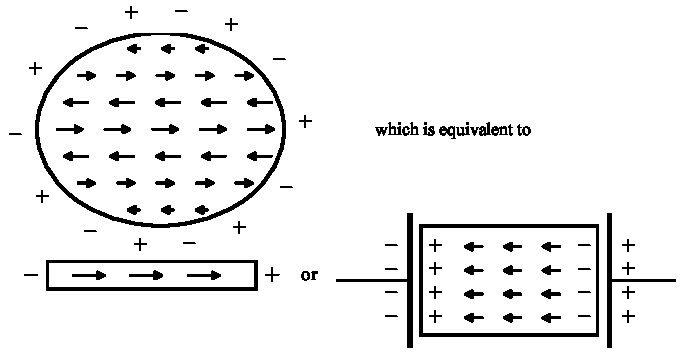
\includegraphics[width=0.72\textwidth]{fig_dipole-t.pdf}
\caption*{无编号插图（原书不编号）　$T_t$ 的等效图像：左为椭球内交替反向的平行偶极子阵列，椭球表面上 +、− 电荷交替排列；右侧旁注 “which is equivalent to”（它等价于）一个充电的平行板电容器，下方旁注 “or”（或），即一根两端各带 −、+ 电荷、内部箭头同向的细棒}
\end{figure}

而 $T_l$ 则是相反的情形，等价于

\begin{figure}[H]
\centering
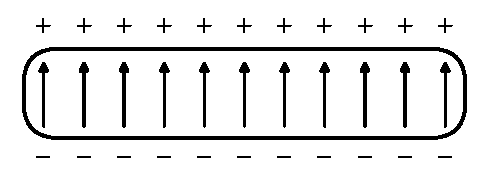
\includegraphics[width=0.72\textwidth]{fig_dipole-l.pdf}
\caption*{无编号插图（原书不编号）　$T_l$ 的等效图像：圆柱内彼此平行的偶极子（箭头一律朝上），上表面排满 + 电荷，下表面排满 − 电荷}
\end{figure}

如图所示。这一差别完全由宏观的表面电荷或体电荷造成，后者可以用宏观介电理论算出。它与 Lyddane、Sachs 与 Teller (85) 等人关于光学声子纵–横频率差的理论完全类似。

为了表明这一切与经典介电理论的直接关系，让我们写下经典电介质的运动方程：

\begin{equation*}
\frac{d^{2}\mathbf{P}}{dt^{2}} \;+\; \omega_0^{2}\,\mathbf{P} \;=\; \beta\, \mathbf{E}_{\mathrm{eff}}
\end{equation*}

这里 $\beta$ 是一个耦合常数，考虑零频率极限便可以用偶极矩阵元把它求出来；在这个极限下，我们从直截了当的微扰论知道，原子系统的极化率为

\begin{equation*}
\alpha \;=\; \frac{2 N X^{2}}{E_0} \;=\; \frac{2 N X^{2}}{\hbar\omega_0} \;=\; \frac{\beta}{\omega_0^{2}}
\end{equation*}

在局域场近似下，原子所感受到的有效场为 $\mathbf{E}_{\mathrm{eff}} = \mathbf{E} + L\mathbf{P}$，其中 $L$ 是“局域场常数”（local-field constant），对立方晶格与横波它取 $4\pi/3$。于是共振频率由

\begin{equation*}
\left(-\omega_r^{2} + \omega_0^{2}\right)\mathbf{P} \;=\; \beta\, L\mathbf{P}
\end{equation*}

决定，并且取 $\omega_r \approx \omega_0$，就得到

\begin{align*}
2\,(\omega_r - \omega_0)\,\omega_0 \;&=\; -\,\beta L \\
\hbar\omega_r \;\simeq\; \hbar\omega_0 \;-\; \frac{\hbar\beta}{2\omega_0}\, L \;&=\; \hbar\omega_0 \;-\; N X^{2} L
\end{align*}

这跟我们用直接的量子力学手段得到的表达式相同。后面我们会看到如何恢复与更完整的经典公式

\begin{equation*}
\frac{\omega^{2} - \omega_0^{2}}{\omega_0^{2}} \;=\; -\,\alpha(\omega{=}0)\cdot L \tag{15'}
\end{equation*}

的相符。

Hopfield 的论文里有一个对整个激子问题的有趣处理，即把一个经典介质作量子化；我不打算在此重述，因为后面讨论自旋波时我们会给出一个类似的处理。

不过，Hopfield 关于激子与辐射相互作用的结果我还是应当讨论一下，因为它们说明了若干有趣的物理要点。到目前为止，我们在计算中只纳入了电磁场中导致 Coulomb 相互作用的纵向部分。横向辐射场与纯纵向的激子并不相互作用，但它当然会通过如下形式的项直接与横向激子耦合：

\begin{equation*}
\sum_{k,\lambda} \left(\mathbf{M}\cdot\mathbf{E}\right)_{k} \left(-\, b_{k\lambda}^{\dagger}\, a_{k\lambda} \;+\; b_{k\lambda}\, a_{k\lambda}^{\dagger}\right)
\end{equation*}

其中 $a_{k\lambda}$ 是光子的产生与湮灭算符，而矩阵元可以证明为

\begin{equation*}
i\left(\frac{2\pi\hbar c}{|k|}\right)^{1/2} \frac{\omega_0}{c}\, X
\end{equation*}

$\lambda$ 是偏振指标。Hopfield 指出，在理想晶体中，我们不应当把这个耦合看作导致光子被激子所吸收，而应当把它看作两个独立的玻色型激发之间的耦合，二者的谱如图 45 所示。激子的速度远远小于

\begin{figure}[H]
\centering
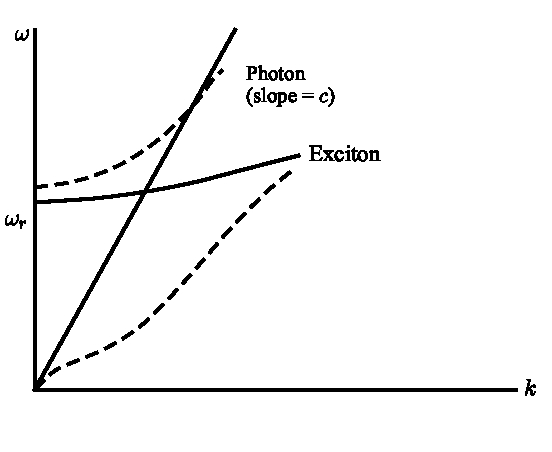
\includegraphics[width=0.72\textwidth]{fig_45.pdf}
\caption*{图 45　光子（直线，斜率 = c）与激子（自 $\omega_r$ 出发的缓升曲线）的色散谱，$\omega$ 轴上标出 $\omega_r$；虚线示引入耦合后谱在交叉点附近发生的劈裂（原书图注仅作 “Figure 45”）}
\end{figure}

光子的速度，因此两支频率在非常小的 $k$ 处相交。自然，当我们引入耦合后，结果便是在交叉点附近两支谱发生劈裂，如图中虚线所示。于是，在没有声子与缺陷的情形下，光子并不被吸收，而是在激子频率处受到强烈色散。对能量处于 $\omega_r$ 附近的辐射，存在一个完全不透明的区域，即截止带（stop band）；在该带的两侧，光子速度被大大减慢。这正是辐射的共振俘获（resonance trapping）现象在固体中的对应物；可以把它想成光子经由反复的吸收与再发射而被减慢乃至停止。当然，在实际晶体中，结果表明通过多声子发射这类过程，激子被吸收的程度远比光子强烈，因而在激子频率附近会发生一个类似吸收的过程。然而必须把这一点理解为从激子-光子混合模式向声子或杂质自由度的直接吸收，而不是光子被激子本身所吸收。

Hopfield 与 Thomas 已经在 CdS 晶体中用实验演示了激子的若干这类性质。通过观察主轴以外方向上的吸收，他们得以造成纵向与横向激子的轻微混合，从而在实验上证实了这两类模式之间的频率差。在另一些安排中，他们借助磁场证明：与光子发生强相互作用的激子确实是以有限的、非零的动量在传播，而不是静止的受激原子；并已在实验上粗略测得激子的速度 (86)。

Frenkel 激子的另一个方面，是高能量偶极项所起的作用；这些项在我们迄今为止的处理中一直被忽略。静电相互作用 (11) 也包含如下形式的偶极矩阵元：

\begin{equation*}
\left(c_j^{p_x}\right)^{\dagger} \left(c_k^{p_x}\right)^{\dagger} c_k^{s}\, c_j^{s} \left(\int a_{p_x}^{*}\, ex\, a_s\right)^{2} \left(T_{jk}\right)_{xx}
\end{equation*}

它们的作用是把原子 $j$ 与原子 $k$ 同时激发。由此在哈密顿量中产生的项，用玻色子 $b$ 写出即为

\begin{gather*}
\frac{X^{2}}{2} \sum_{j\neq k} b_j^{\dagger}(1-n_j)\cdot T_{jk}\cdot b_k^{\dagger}(1-n_k) \\
+\; \frac{X^{*2}}{2} \sum_{j\neq k} (1-n_j)\, b_j\cdot T_{jk}\cdot(1-n_k)\, b_k \tag{16}
\end{gather*}

在大多数情形下我们可以取 $X$ 为实数。（译注：上式第二行的求和限原书印作 $i\neq k$，显系 $j\neq k$ 之误排，此处径改。）

眼下最显而易见的做法，是用微扰论来处理这些项，同时十分有理由地假定相应激发态的平均能量恰好就是 $2E_0$。我们得到固体总能量降低了

\begin{equation*}
\Delta E_2 \;=\; -\, \frac{N|X|^{4}}{2E_0} \sum_j T_{0j}:T_{0j}
\end{equation*}

它正比于 $R_{0j}^{-6}$，显然恰恰应当把它等同于原子间 Van der Waals 吸引中来自这一特定电子跃迁的分量——也就是按独立原子计算出来的那一份。

用另一种方式来做这件事是有趣的。我们看到，在用较简单的哈密顿量 (15) 考虑\emph{第一个}激子时，激子算符运动方程中的非线性项恰好为零。因此在那一级近似下，第一个激子是系统的一个\emph{精确}激发态。现在我们做出典型的“元激发”假设：即使存在物理上数量可观的元激发，元激发之间的相互作用也可以在某级近似下予以忽略；也就是说，无论在 (15) 中还是在我们现在所考虑的 (16) 的各项中，都把 $(1-n_j)$ 换成 1，只保留玻色子振幅的二次项。

必须认识到，一旦把 (16) 计入哈密顿量，就连基态也会含有原子激发态的小振幅，因为存在一些被激发而又退激发的激子对。这个百分比实际上并不微不足道，

% ——上句在原书 p144 末中断于 “The percentage is not in fact”，p145（PDF p160）起由后续代理续译衔接。

% 衔接说明：本文件首段承上文件 ch3_D1b.tex 末句——原书 p144 末句 "The percentage
% is not in fact" 与本文件首词 “微不足道” 合成完整一句（“这个百分比实际上并不微不足道”）。
% 本文件止于原书 p156 末的 $\delta(q,q')$ 等式；原书 p157 顶部（D.2 小节标题之前）
% 尚有一段 D.1 收尾文字，已暂存于 ch3_D2.tex 顶部（%--D1-TAIL-- 标记之下），
% 装配时应接于本文件之后。

%JOIN%
因为在较好的稀有气体和离子晶体中，$X^{2}T_{jk}$ 约为 1/2 至 1 eV，所以该振幅是 0.1 的量级。因此，令 $n_j = 0$ 确实是一个有实质内容的假定，不过在这个情形下也是一个相当准确的假定。

那么，就让我们在这个线性化近似下，把新的、完整的哈密顿量用玻色子算符 $\beta_{k\lambda}$ 表示出来（$\lambda$ 标记激子的偏振）：

\begin{gather*}
\mathcal{H} \;=\; \sum_{k\lambda} \left(E_0 + X^{2}\,T_{\lambda}(k)\right) \beta_{k\lambda}^{\dagger}\,\beta_{k\lambda} \\
+\;\sum_{k\lambda} X^{2}\,T_{\lambda}(k)\left(\beta_{k\lambda}^{\dagger}\,\beta_{-k\lambda}^{\dagger} + \beta_{k\lambda}\,\beta_{-k\lambda}\right) \tag{17}
\end{gather*}

让我们试着把它对角化。显然，唯一的途径是把算符 $\beta_k^{\dagger}$ 与 $\beta_{-k}$ 混合起来，反之亦然——这种做法读者如今已从超导理论中熟悉了。［其实，相应的变换很可能最早就是 Bogolyubov 在 $\mathrm{He}^{4}$ 理论中作出的 (87)。］于是我们令

\begin{gather*}
\beta_k^{\dagger} \;=\; u_k B_k^{\dagger} - v_k B_{-k} \qquad\qquad \beta_k \;=\; u_k B_k - v_k B_{-k}^{\dagger} \\
\beta_{-k}^{\dagger} \;=\; u_k B_{-k}^{\dagger} - v_k B_k \qquad\qquad \beta_{-k} \;=\; u_k B_{-k} - v_k B_k^{\dagger}
\end{gather*}

为保证这些新算符遵守玻色子的对易规则，我们只需检验

\begin{equation*}
\left[\,\beta_k,\;\beta_k^{\dagger}\right] = 1 \qquad\text{若}\qquad \left[\,B,\;B^{\dagger}\right] = 1
\end{equation*}

也就是说，

\begin{equation*}
u_k^{2}\left[\,B_k,\,B_k^{\dagger}\right] + v_k^{2}\left[\,B_{-k}^{\dagger},\,B_{-k}\right] = 1
\end{equation*}

或者，

\begin{equation*}
u_k^{2} - v_k^{2} = 1
\end{equation*}

只要令

\begin{equation*}
u_k \;=\; \cosh\frac{\theta_k}{2} \qquad\qquad v_k \;=\; \sinh\frac{\theta_k}{2}
\end{equation*}

它便自动得到满足。

现在让我们代入哈密顿量 (17) 之中。其中特定的一组项可以写成

\begin{equation*}
E_k^{0}\left(\beta_k^{\dagger}\beta_k + \beta_{-k}^{\dagger}\beta_{-k}\right) + E_k'\left(\beta_k^{\dagger}\beta_{-k}^{\dagger} + \beta_{-k}\beta_k\right)
\end{equation*}

这些项现在变为

\begin{align*}
E_k^{0}\,\Bigl\{\; & u_k^{2}\left(B_k^{\dagger}B_k + B_{-k}^{\dagger}B_{-k}\right) + v_k^{2}\left(B_{-k}B_{-k}^{\dagger} + B_k B_k^{\dagger}\right) \\
& -\; 2u_k v_k\,\left[B_k^{\dagger}B_{-k}^{\dagger} + B_{-k}B_k\right]\Bigr\} \\
+\; E_k'\,\Bigl\{\; & \left(u_k^{2} + v_k^{2}\right)\left(B_k^{\dagger}B_{-k}^{\dagger} + B_{-k}B_k\right) \\
& -\; u_k v_k\left(B_k^{\dagger}B_k + B_{-k}B_{-k}^{\dagger} + B_{-k}^{\dagger}B_{-k} + B_k B_k^{\dagger}\right)\Bigr\}
\end{align*}

这样，只要令

\begin{equation*}
\frac{2u_k v_k}{u_k^{2} + v_k^{2}} \;=\; \tanh\theta_k \;=\; \frac{E_k'}{E_k^{0}} \tag{18}
\end{equation*}

哈密顿量便被对角化了。

其余各项，在利用

\begin{equation*}
B_k B_k^{\dagger} \;=\; B_k^{\dagger} B_k + 1
\end{equation*}

之后，便可以写成

\begin{equation*}
\left[E_k^{0}\left(u_k^{2} + v_k^{2}\right) - 2u_k v_k E_k'\right]\left(n_k + n_{-k}\right) + 2\left(v_k^{2}E_k^{0} - u_k v_k E_k'\right)
\end{equation*}

于是，激子的新能量为

\begin{equation*}
E_k \;=\; E_k^{0}\cosh\theta_k - E_k'\sinh\theta_k
\end{equation*}

但根据 (18)，我们可以令

\begin{gather*}
E_k^{0} \;=\; E_k\cosh\theta_k \\
E_k' \;=\; E_k\sinh\theta_k
\end{gather*}

并可核实

\begin{equation*}
E_k \;=\; E_k\left(\cosh^{2}\theta_k - \sinh^{2}\theta_k\right)
\end{equation*}

进而得到

\begin{equation*}
E_k \;=\; \frac{E_k^{0}}{\cosh\theta_k} \;=\; E_k^{0}\left(1 - \tanh^{2}\theta_k\right)^{1/2} \;=\; \Bigl\{\left(E_k^{0}\right)^{2} - \left(E_k'\right)^{2}\Bigr\}^{1/2}
\end{equation*}

这一整套操作，与人们对角化 B.C.S. 哈密顿量 (88) 时所经历的步骤极为相似，只不过对玻色子来说，起作用的是双曲函数而不是三角函数，而且根号下的符号也相应地不同。Suhl（私人通信）曾作为一个有趣的练习，用玻色对算符（boson-pair operators）

\begin{equation*}
\beta_k^{\dagger}\beta_{-k}^{\dagger}\,, \qquad \beta_k^{\dagger}\beta_k + \beta_{-k}^{\dagger}\beta_{-k}\,, \qquad \beta_{-k}\beta_k
\end{equation*}

把这类哈密顿量对角化。这些玻色对算符具有双曲空间中而非实空间中的自旋所具有的性质——也就是说，它们像 $S$ 取虚值的自旋，对应于虚数阶的 Legendre 函数。

我们还看到，随着激子频率的降低，总能量也有所下降；这一下降可以被非常直接地解释为激子零点能相应的降低。利用恒等式

\begin{equation*}
v^{2} \;=\; \frac{u^{2} + v^{2} - 1}{2} \qquad\qquad \text{（由}\;\; u^{2} - v^{2} = 1\;\;\text{而来）}
\end{equation*}

我们得到

\begin{equation*}
\Delta E \;=\; \sum_{k}\left(E_k - E_k^{0}\right) \tag{19}
\end{equation*}

于是，经过完全对角化的总哈密顿量为

\begin{align*}
\mathcal{H} \;=\; \sum_{k>0,\,\lambda} \Bigl\{ & \left(E_0 + X^{2}T_{k\lambda}\right)^{2} - \left(X^{2}T_{k\lambda}\right)^{2}\Bigr\}^{1/2} \left(n_{k\lambda} + \frac{1}{2} + n_{k\lambda} + \frac{1}{2}\right) \\
& -\;\sum_{k\lambda}\left(E_0 + X^{2}T_{k\lambda}\right)
\end{align*}

（译注：第一个括号中第二个 $n_{k\lambda}$ 照录原书；按上下文应为 $n_{-k\lambda}$，如此对 $k>0$ 求和方能给出与 $k$ 与 $-k$ 两支模相应的零点项。）

其中 $n_{k\lambda} = B_{k\lambda}^{\dagger}B_{k\lambda}$。注意 $E_k = \left(E_0^{2} + 2E_0 X^{2}T_k\right)^{1/2}$。这显然与 (15$'$) 相同。

在这种表述中，我们使一个由 Hopfield 指出的相当有趣的事实变得一目了然：分子晶体的结合能可以重新解释为激子因偶极相互作用而导致的零点能之下降，因为它主要是 Van der Waals 吸引。

关于这个零点能问题，有一个相当重要的论点值得作些讨论。在我们原来的哈密顿量中，除了纯原子项 $(E_0/2)\left(c_p^{\dagger}c_p - c_s^{\dagger}c_s\right)$ 之外，其余各项都只涉及不同原子上的激子算符，而这些项当然是自动对易的。我们总是选择把它们写成 $b_j^{\dagger}b_k$ 的次序，结果得到的哈密顿量中含有 $E_k^{0}\,\beta_k^{\dagger}\beta_k$。这就是上面出现的那个减除项［即 (19) 中的 $-E_k^{0}$ 项］。当然，这一做法虽然是对我们实际物理情形的正确描述，却并不是经典介电连续介质在正确量子化下应有的哈密顿量；后者本应以对称化的形式出现：

\begin{equation*}
\frac{E_k^{0}}{2}\left(\beta_k^{\dagger}\beta_k + \beta_k\beta_k^{\dagger}\right)
\end{equation*}

由于我们所假设的系统与经典介电连续介质并没有明显的物理相似之处，这一点本来不必使我们过于担心；而事实上结果表明它无论如何也是对的。如果我们想采用对称化的形式，就必须补加 $\sum_k E_k^{0}$；鉴于 $\sum_k T_k = 0$，这个补项只依赖于纯原子的量 $E_0$，与相互作用毫无关系。当然，这个恒等式之所以成立，恰恰是因为我们本来就没有 $j=k$ 的相互作用项；这也正是我们一开始便能任意选择算符次序的原因。在自旋波问题和声子问题中，经典出发点与量子出发点之间的这种关系将更为切题。

现在让我们开始离开严格局域化的 Frenkel 激子这一主题，进而考虑这样的可能性：尽管受到对方 Coulomb 场的作用，受激电子或空穴偶尔仍会离开它的同伴而游走。这意味着我们必须在哈密顿量中计入如下各项：

\begin{equation*}
\mathcal{H}' \;=\; \sum_{jk}\left[b_{jk}^{s}\,c_j^{s\dagger}\,c_k^{s} + b_{jk}^{p}\,c_j^{p\dagger}\,c_k^{p}\right] \tag{20}
\end{equation*}

但同时我们还必须计入能量差 $U$；当受激电子与空穴处于同一原子上时，正是这个能量差使受激电子的能量降低：

\begin{equation*}
\mathcal{H}_{\mathrm{int}} \;=\; U\sum_j n_j^{p}\,n_j^{s} \tag{21}
\end{equation*}

对于 (20) 中的各项，我们所能采取的最好办法是用微扰论来处理：从 $U\to\infty$ 的极限出发，求出 $b^{2}/U$ 量级的第一级修正。在 U 非常大的极限下，合适的做法是考察 Coulomb 相互作用 (21) 的本征态。这些本征态按照同一原子上共有 0 对、1 对、2 对……s 电子与 p 电子而自行形成一个分层结构，其能量分别为 0、U、2U……迄今为止，我们处理的只是这类态中 $U = 0$ 的简并子空间，即电子与空穴占据同一原子的那些态；这些态已被偶极相互作用劈开，而这一劈裂与 U 相比显然很小。下一步要计算的，是这个简并子空间因虚跃迁而产生的进一步劈裂；在虚跃迁中，电子或空穴会跳到一个已经有另一粒子所在的原子上，这在 U 非常大的极限下具有能量 U。显然，为了得到最低阶的效应，我们不能容许电子继续游荡，而必须强迫它在下一次跳跃时就回到自己的空穴处。于是，我们把微扰级数

\begin{equation*}
\mathcal{H}_{\mathrm{eff}} \;=\; \mathcal{H}' - \mathcal{H}'\,\frac{1}{U}\,\mathcal{H}' + \mathcal{H}'\,\frac{1}{U}\,\mathcal{H}'\,\frac{1}{U}\,\mathcal{H}' \cdots
\end{equation*}

投影到由“允许”态（即电子与空穴在一起的态）构成的子空间 $|0\rangle$ 上：

\begin{equation*}
\mathcal{H}^{(2)} \;=\; -\left\langle 0\right|\,\mathcal{H}'\,\frac{1}{U}\,\mathcal{H}'\,\left|0\right\rangle
\end{equation*}

并略去一切更高阶的微扰。只要只保留电子或空穴返回其原来所在原子的那些项，这一点便很容易做到；(20) 与 (21) 的二级效应于是为

\begin{align*}
\mathcal{H}^{(2)} \;=\; -\frac{1}{U}\sum_{jk}\Bigl[\; & b_{jk}^{s}\left(c_j^{s}\right)^{\dagger}c_k^{s} + b_{jk}^{p}\left(c_j^{p}\right)^{\dagger}c_k^{p}\,\Bigr] \\
\times\,\Bigl[\; & b_{kj}^{s}\left(c_k^{s}\right)^{\dagger}c_j^{s} + b_{kj}^{p}\left(c_k^{p}\right)^{\dagger}c_j^{p}\,\Bigr] \\
=\; -\frac{1}{U}\sum_{jk}\Bigl\{\; & |b_{jk}^{s}|^{2}\,n_j^{s}\left(1 - n_k^{s}\right) + |b_{jk}^{p}|^{2}\,n_j^{p}\left(1 - n_k^{p}\right) \\
& +\; b_{jk}^{s}\,b_{kj}^{p}\left(c_j^{s}\right)^{\dagger}c_k^{s}\left(c_k^{p}\right)^{\dagger}c_j^{p} \;+\; \mathrm{c.c.}\Bigr\}
\end{align*}

（译注：第二个方括号内 $\left(c_k^{p}\right)$ 上的产生算符符号 $^{\dagger}$ 原书漏印，此处按对称性补出。）

前两项有些不对称，所以我们在 jk 与 kj 这两对指标之间把它们对称化。同时我们还考虑到如下事实：在我们所考虑的 $|0\rangle$ 态流形之内，$n_j^{p} = 1 - n_j^{s}$，反之亦然——每个原子上要么有一个受激电子，要么有一个基态电子。于是，对这两项我们得到

\begin{equation*}
-\frac{1}{U}\sum_{jk}\frac{|b_{jk}^{s}|^{2} + |b_{jk}^{p}|^{2}}{2}\left(n_j^{s}n_k^{p} + n_j^{p}n_k^{s}\right)
\end{equation*}

用激子算符来表示，

\begin{align*}
n_j^{s}n_k^{p} + n_j^{p}n_k^{s} \;&=\; \frac{1}{2}\left(n_j^{s} + n_j^{p}\right)\left(n_k^{s} + n_k^{p}\right) - \left(n_j^{p} - n_j^{s}\right)\left(n_k^{p} - n_k^{s}\right) \\
&=\; \frac{1}{2}\left(1 - \sigma_z^{j}\sigma_z^{k}\right)
\end{align*}

或者

\begin{equation*}
=\;2\left(-\,n_j n_k + n_j + n_k\right)
\end{equation*}

后一种形式表明，这一项除了给出相邻激子之间的一个非线性相互作用之外，还使激子的能量降低

\begin{equation*}
\frac{1}{U}\sum_{K}\left\{|b_{jk}^{s}|^{2} + |b_{jk}^{p}|^{2}\right\}
\end{equation*}

（译注：求和限 $K$ 原书如此（大写），按上下文应为 $jk$。）

$\sigma$ 形式在自旋波问题中将会很重要。

激子能量中的这个对角项并不十分重要；它所反映的事实是：$b$ 项把自由粒子的各个能级展宽成为一个能带，从而把激子的平均能量压低。另一项则更有意思；它恰好具有导致激子运动的那些偶极项的形式，因此我们可以把这些项写成与偶极项相类似的形式：

\begin{gather*}
\mathcal{H}^{(2)} \;\simeq\; -\sum_{jk} T_{jk}'\,b_j^{\dagger}\,b_k \\
T_{jk}' \;=\; \frac{b_{jk}^{s}\,b_{jk}^{p}}{U} \tag{22}
\end{gather*}

这里涉及的机制显然是：电子先虚跳到相邻的原子上，随后空穴再朝同一方向跳过去。这种迁移机制对光学活性的 Frenkel 激子并不十分重要，但对禁戒的激子却相当重要，对自旋波尤其如此。显然，这一效应的效果是使激子谱略微跟上由 $b_{jk}$ 引起的单粒子谱的展宽（图 46）。一旦 b 大到足以与 U 相比，这个模型就完全失效了。当 b 增大时我们看到，激子态的能量减小约 $Zb^{2}/U$；另一方面，最低的一些能带态——也就是最能利用与近邻之间正确相位关系的那一些态——其能量则减小约 $Zb$。于是，在这个模型中激子的结合能按如下方式减小：

\begin{equation*}
\mathrm{BE} \;\cong\; U - Zb + \frac{Zb^{2}}{U}
\end{equation*}

\begin{figure}[H]
\centering
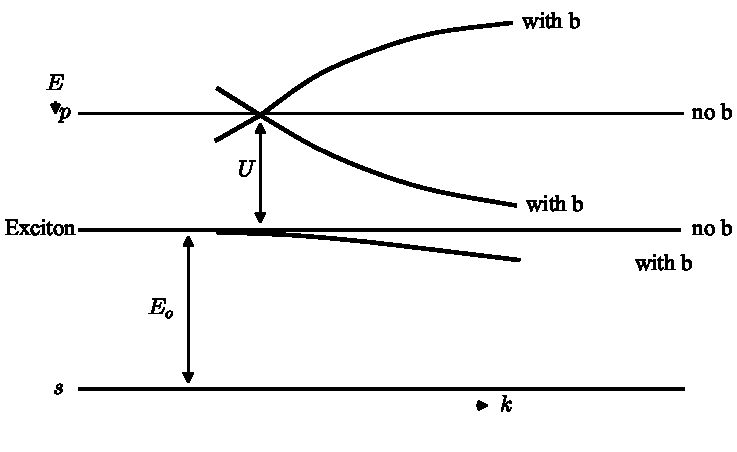
\includegraphics[width=0.72\textwidth]{fig_46.pdf}
\caption*{图 46　能级示意：p 能级与激子（Exciton）能级各给出 no b（不计 $b$，水平直线）与 with b（计入 $b$，曲线）两种情形；$U$ 标出 p 组态与激子组态之间的能量间隔，$E_0$ 为自 s 能级到激子能级的间距，左侧箭头 $E$ 指示能量向下减小，横轴为 $k$（原书图注仅作 “Figure 46”）}
\end{figure}

因此，一旦 $bZ \sim U$，纯局域激子的能量就未必低于带边（图 47）；那时我们将不得不只用能量极小点附近的电子态来构成激子态，才有希望得到低于能带连续谱的激子。此外，在一个 b 相当可观的材料中，Wannier 函数更为扩展，而介电屏蔽会使 U 的作用减弱。于是我们预期，随着 $b/U$ 的变化，会发生一次相当陡峭的转变，转到激子理论的相反情形，即 Wannier 极限：在这种极限下，电子与空穴很少同时处于同一原子上，而是具有一个可以由能带极小附近的态构成的长程波函数。

\begin{figure}[H]
\centering
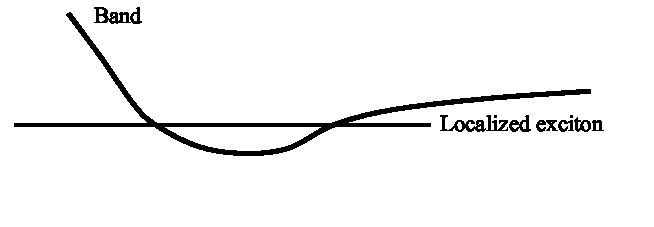
\includegraphics[width=0.72\textwidth]{fig_47.pdf}
\caption*{图 47　向下弯曲的 “Band”（能带）曲线与 “Localized exciton”（局域激子）水平能级线相交示意（原书图注仅作 “Figure 47”）}
\end{figure}

这种情形可以用能带理论的“有效单带哈密顿量”（effective one-band hamiltonian）方法来处理——事实上，Wannier 在 1937 年正是从这个问题出发开创了这一理论的近代发展 (78)。我们采用近似哈密顿量

\begin{equation*}
\mathcal{H}_{\mathrm{eff}} \;=\; E_{\mathrm{el}}(k_e) + E_{\mathrm{hole}}(k_h) + \frac{e^{2}}{\kappa\,|R_e - R_h|}
\end{equation*}

一般说来，这会导致相当复杂的方程，尽管原则上并非不可处理。在简并能带的情形下尤其如此，那时甚至连质心运动也不容易分离出来。幸运的是，最有趣的那些情形恰好也是激子相当容易被观察到的情形，而这些情形看来都是简单的有效质量椭球（effective mass ellipsoid）情形；在这种情形下我们可以写出

\begin{equation*}
\mathcal{H} \;=\; -\frac{\hbar^{2}}{2}\sum_{\alpha=x,y,z}\frac{1}{m_{\alpha e}}\frac{\partial^{2}}{\partial x_{\alpha e}^{2}} + \frac{1}{m_{\alpha h}}\frac{\partial^{2}}{\partial x_{\alpha h}^{2}} - \frac{e^{2}}{\kappa\,|R_e - R_h|}
\end{equation*}

并且质心运动与相对运动可以分离开来，给出描写整体运动的激子质量张量 $\left(m_e + m_h\right)_{\alpha}$，以及描写相对运动的约化质量张量

\begin{equation*}
\left(\frac{m_e m_h}{m_e + m_h}\right)_{\alpha}
\end{equation*}

即使这一点做不到——例如出现简并，或者椭球的主轴互不相同——往往也会有一个粒子比另一个重得多，从而可以找到良好的近似。

于是，激子在坐标表象中的波函数为

\begin{equation*}
\Psi \;=\; \Phi(R_e - R_h)\;e^{iq\left(R_e + R_h\right)}
\end{equation*}

其中 q 是质心运动的波数。相对于原子间距而言，$\Phi$ 是一个相当长程的函数。把这一处理中所作的近似与我们前面 Frenkel 处理中的近似作一对比，并用图示来说明激子在这两种情形下如何运动，是有趣的。让我们把两个能带——电子（导）带与空穴（价）带——中 Wannier 函数的产生算符分别记为 $w_e^{\dagger}(R_j)$ 与 $w_h^{\dagger}(R_j)$；例如，$w_e$ 定义为

\begin{equation*}
w_e^{\dagger}(\mathbf{R}_j) \;=\; \int a_e(r - \mathbf{R}_j)\,\psi^{\dagger}(r)\;dr
\end{equation*}

这里 e 表示空带。波函数 $\Psi$ 可以写成

\begin{equation*}
\Psi \;=\; \sum_{jk}\phi_q(R_j - R_k)\;e^{iq\cdot\left(R_j + R_k\right)}\;w_e^{\dagger}(\mathbf{R}_j)\,w_h(\mathbf{R}_k)\,\Psi_g
\end{equation*}

而这个近似哈密顿量相当于在相互作用能中只保留

\begin{equation*}
\frac{e^{2}}{\kappa\,|R_j - R_k|}\;n_e(R_j)\,n_h(R_k)
\end{equation*}

并忽略一切非对角元。于是在这种情形下，相互作用根本不引起任何运动：$w_e^{\dagger}(j)\,w_h(k)\,\Psi_g$ 就是这一相互作用的一个本征函数，其能量为

\begin{equation*}
-\frac{e^{2}}{\kappa\,|R_j - R_k|}
\end{equation*}

运动反而完全来自哈密顿量中的 $b_{jk}$ 各项。我们可以用一幅以时间 t 对位置 x 作图的图来描述它：相互作用发生在电子与空穴位置固定之处，而两次相互作用之间这两个粒子在 x 空间中运动（图 48）。这些相互作用只在长距离处发生，其唯一的效果就是把电子与空穴维系在一起。

\begin{figure}[H]
\centering
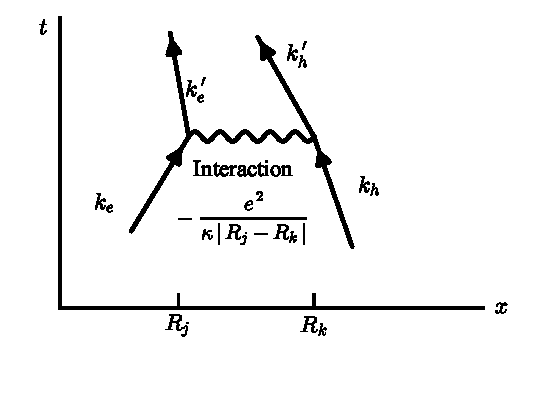
\includegraphics[width=0.72\textwidth]{fig_48.pdf}
\caption*{图 48　时间 $t$–位置 $x$ 图：电子（$k_e$）与空穴（$k_h$）的径迹在固定位置 $R_j$、$R_k$ 之间由一条波线相连，波线标 “Interaction”（相互作用）$-e^{2}/\kappa|R_j - R_k|$，作用后两径迹以 $k_e'$、$k_h'$ 继续（原书图注仅作 “Figure 48”）}
\end{figure}

在另一种情形中，我们假定 $b_{jk}$ 为零，电子与空穴完全不能移动；唯一的例外是 $w_h$ 与 $w_e^{*}$ 可以彼此湮灭，其矩阵元为 X［见图 49(a)］。图 49(b) 中画出的，是由式 (22) 所描述的经由电子或空穴一次虚跳的运动；它与图 48 的过程密切相关。图 49(a) 所示的那种图也会在 Wannier 激子中出现，但只在电子与空穴的路径偶然相交这一罕见事件中才会发生（图 50）。该图表明这样一个事实：与外场相互作用的有效偶极矩——其图解如图 51 所示——要被缩小为激子态体积的倒数，因为只有当电子与空穴彼此靠近时湮灭才会发生。由此造成的纵–横频率差相当小。它无法单靠有效哈密顿量理论来处理。

\begin{figure}[H]
\centering
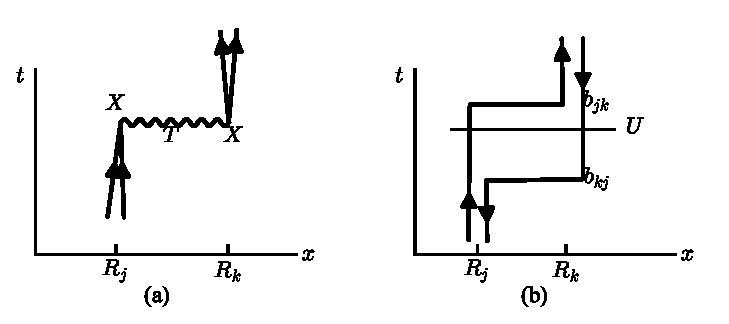
\includegraphics[width=0.72\textwidth]{fig_49.pdf}
\caption*{图 49　$t$–$x$ 图两种情形：(a) 电子与空穴的径迹在 $R_j$ 与 $R_k$ 处各标一次 “X”，其间由标 “T” 的波线相连，两端各有向上的箭头；(b) 虚跳图：标 $b_{jk}$ 与 $b_{kj}$ 的竖直跳变跨过标 $U$ 的水平线（原书图注仅作 “Figure 49”）}
\end{figure}

\begin{figure}[H]
\centering
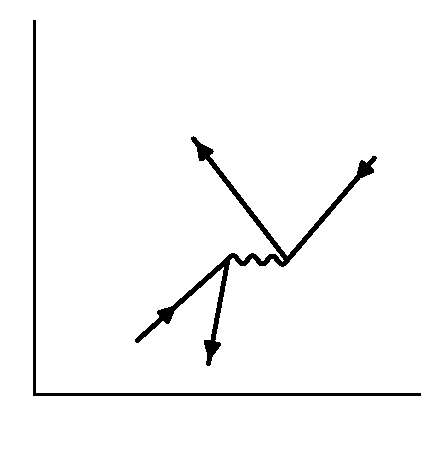
\includegraphics[width=0.72\textwidth]{fig_50.pdf}
\caption*{图 50　Wannier 激子中电子与空穴路径偶然交叉时的相互作用图（$t$–$x$ 图，交叉点处接波线）（原书图注仅作 “Figure 50”）}
\end{figure}

\begin{figure}[H]
\centering
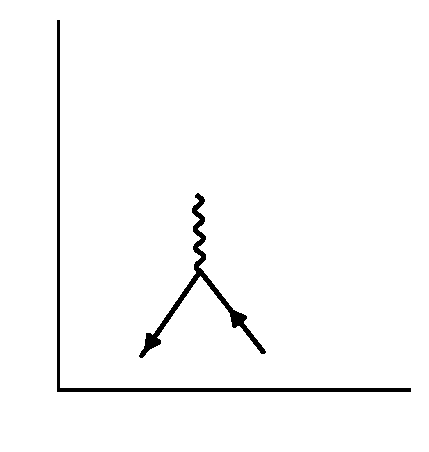
\includegraphics[width=0.72\textwidth]{fig_51.pdf}
\caption*{图 51　与外场相互作用的顶点图：一条波线（外场量子）在同一个时空点上与电子、空穴的径迹相接（原书图注仅作 “Figure 51”）}
\end{figure}

看待我们对基态能量以及 Frenkel 激子频率所作的那些零点修正的一种方式，是注意到它们相当于在激子的传播方程中计入了所谓的“反向图”（backwards diagrams）（见图 52）。这类“反向图”在核多体理论和核能级结构中的效应要大得多 (89)。这些图例示了在多体理论中对图的子集求和的过程。

\begin{figure}[H]
\centering
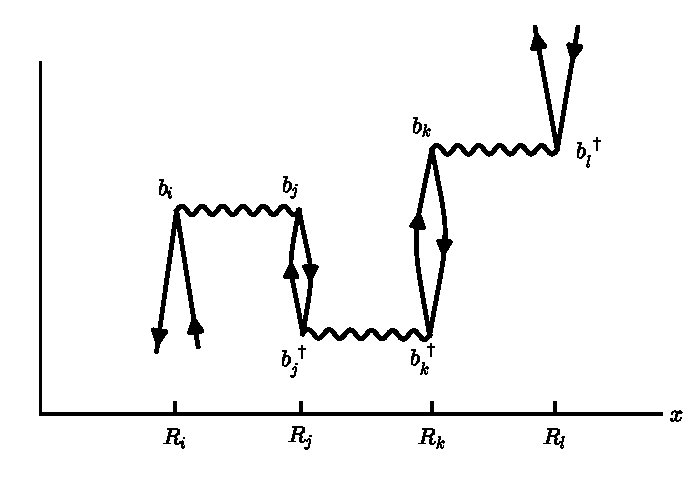
\includegraphics[width=0.72\textwidth]{fig_52.pdf}
\caption*{图 52　“反向图”示意：电子与空穴的径迹在 $R_i$、$R_j$、$R_k$、$R_l$ 各处经波线相互作用，中间形成两个环状结构，各段标以 $b_i$、$b_j$、$b_j^{\dagger}$、$b_k$、$b_k^{\dagger}$、$b_l^{\dagger}$（原书图注仅作 “Figure 52”）}
\end{figure}

像图 48 那样的图称为“梯图”（ladder diagrams）；对两个粒子求解 Schrödinger 方程，就等价于“把梯图求和到无穷阶”——也就是说，允许这种隔距相互作用按需要的次数、实质上连续不断地起作用。像图 49 那样的图则常称为“泡图”（bubble）或“环图”（ring），它们与材料的介电常数有关。在激子这个简单情形中，除了某种程度的数学复杂性之外，其实没有什么东西妨碍我们把两组图一起求和；我们已经给出了两类求和分别更为重要的那些极限情形。在更复杂的集体激发情形中，也许只能单独地“求和”梯图或泡图。在“泡图”的情形下，通常还必须把“反向”图也一并求和；这一步由无规相位近似（random-phase approximation）完成 (90)。

对 Wannier 型的激子来说，没有什么特别明显或简单的方式可以直接过渡到玻色子算符。相反，我们必须遵循较为就事论事的（ad hoc）做法：写下激子算符，然后直接验证，在\emph{只有很少数激发被占据的态}中，它们的对易规则近似地就是玻色子的对易规则。产生一个 Wannier 激子的算符可以写成

\begin{equation*}
O^{\dagger}(q) \;=\; \sum_{jk}\phi_q(j-k)\;e^{iq\cdot\left(\mathbf{R}_j + \mathbf{R}_k\right)}\;w_e^{\dagger}(\mathbf{R}_j)\,w_h(\mathbf{R}_k)
\end{equation*}

于是我们得到

\begin{align*}
\left[O(q),\,O^{\dagger}(q')\right] =\; & \sum_{jklm}\phi_q(j-k)\,\phi_{q'}(l-m)\;e^{iq\cdot\left(\mathbf{R}_j - \mathbf{R}_k\right)\,-\,iq'\cdot\left(\mathbf{R}_l + \mathbf{R}_m\right)} \\
\times\; & \left[\,w_h^{\dagger}(\mathbf{R}_l)\,w_e(\mathbf{R}_m),\;w_e^{\dagger}(\mathbf{R}_j)\,w_h(\mathbf{R}_k)\,\right]
\end{align*}

把这个对易子作用到基态 $\Psi_g$ 上时，除非 $R_j = R_m$、$R_k = R_l$，否则它将为零，因为基态中\emph{从一开始}就不存在任何激子。这意味着 $n_h = 1$、$n_e = 0$；也就是说，除非 l 上有一个空穴、\emph{且} m 上有一个受激电子，否则 $w_h^{\dagger}\,w_e = 0$。在该情形下，对易子的值为 1。在激子情形中，甚至从物理上讲，人们也很少会达到使这一假设失效的态，或许在某些光学微波激射器（optical maser）中除外。于是

\begin{align*}
\left[O(q),\,O^{\dagger}(q')\right]\;&=\;\sum_{j,k}\phi_q(R_j - R_k)\,\phi_{q'}(R_j - R_k)\;e^{i(q-q')\cdot\left(R_j + R_k\right)} \\
&=\;\delta(q,\,q')
\end{align*}

因此，把 Wannier 激子当作玻色子来处理是完全合理的。关于由费米子对组成的激发是否可以、以及何时可以当作玻色子来处理这一普遍问题，最详尽的论述见于 Blatt 与 Matsubara 最近的工作；它读起来相当艰涩，但看来确实厘定了这样的事实：这类激发几乎总是可以这样处理。

\subsection{自旋波：Heisenberg 哈密顿量与“磁状态”}

绝缘体中的自旋波不过是 Frenkel 激子的一种修改与推广。它们是这样一种激子：其中未被占据的或“上面的”带并不是 Hartree-Fock 势中一个独立的轨道带，而正是电子由之被激发出来的那同一个带，只不过自旋相反。要理解这一点何以可能，我们必须简要地讨论一下绝缘体中“磁状态”的结构 (91)。

让我们从最简单的情形，即铁磁绝缘体开始；也就是说，我们假定一个 Hartree-Fock 解——不必是最低的那个解，但须自洽——把第 $n$ 个带中所有自旋向上的态全部填满，而所有自旋向下的态全部空着。

\begin{equation*}
\Psi_{\mathrm{HF}} \;=\; \prod_k \bigl(c^{\,n}_{k\uparrow}\bigr)^{\dagger}\, \Psi_{\mathrm{vac}} \;=\; \prod_j \bigl(w^{\,n}_{j\uparrow}\bigr)^{\dagger}\, \Psi_{\mathrm{vac}}
\end{equation*}

其中这两个表达式是等价的（$c$ 是 Bloch 函数的产生算符，$w$ 是 Wannier 函数的产生算符），因为该带是满带。

读者当还记得，在 Frenkel 激子的情形中，我们作为零级近似出发时取了一个原子激发能 $E_0$，它比带激发能 $E_e - E_h$ 小一个量 $U$，这个 $U$ 代表上、下两个带的 Wannier 函数中处于同一原子上的两个电子之间的排斥能。

撇开原子间的相互作用不谈，在磁性情形中 $E_0$ 必须为零，因为被激发的电子进入的正是基态电子原先所在的同一轨道。也就是说，在这一阶段，把一个自旋就地翻转（\emph{in situ}）并不耗费能量，只有把自旋翻转、同时又把电子移到邻近的原子上去才需要能量。若 Wannier 函数为 $a(r-R_j)$，则能量 $U$ 为

\begin{equation*}
U \;=\; \int \frac{e^{2}}{|r_1 - r_2|}\, dr_1\, dr_2\;\, |a(r_1)|^{2}\, |a(r_2)|^{2}
\end{equation*}

显然，磁状态要有任何意义，第一个先决条件就是 $U$ 必须大，特别是相对于“跳跃”即动能积分

\begin{equation*}
b_{jk} \;=\; \int a^{*}(r-R_j)\, \mathcal{H}\, a(r-R_k)\, dr
\end{equation*}

而言要大。

$U$ 必须很大，这一点可以再次通过考虑铁磁情形看出，此时在能量中只计入以下两项：

\begin{equation*}
\mathcal{H}_0 \;=\; \sum_{jk\sigma} b_{jk}\, w^{\dagger}_{j\sigma}\, w_{k\sigma} \;+\; U \sum_j n_{j\uparrow}\, n_{j\downarrow}
\end{equation*}

我们可以在 Hartree-Fock 近似下处理 $H_0$，假定把所有自旋向上的态都填满，使得 $\langle n_{j\uparrow}\rangle = 1$、$\langle n_{j\downarrow}\rangle = 0$。在这个势中，空穴态的能量当然就是

\begin{equation*}
E(k) \;=\; \sum_j\, e^{ik\cdot R_j}\, b_{0j}
\end{equation*}

而电子态的能量则是 $U + E(k)$（图 53）。
\begin{figure}[H]
\centering
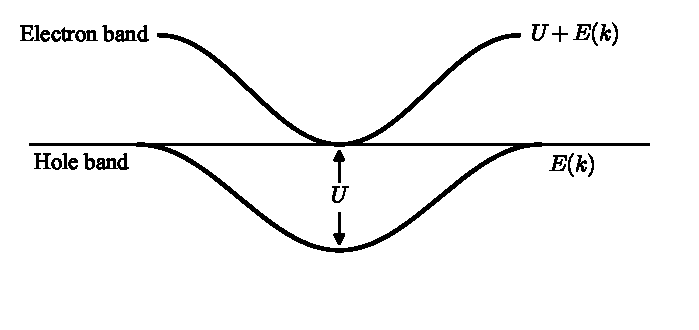
\includegraphics[width=0.66\textwidth]{fig_53.pdf}
\caption*{图 53　（原书图注仅作 “Figure 53”）电子带与空穴带示意：上方曲线为电子带 $U+E(k)$，下方曲线为空穴带 $E(k)$，两曲线极小值之间的竖直箭头标出间隔 $U$}
\end{figure}
这种局面显然只有在所有电子态都位于所有空穴态之上时才是稳定的，即

\begin{equation*}
\bigl[E(k)\bigr]_{\max} \;<\; U \;+\; \bigl[E(k)\bigr]_{\min}
\end{equation*}

这是电子不至于自发地从自旋向上的态转入自旋向下的态、从而把铁磁绝缘体变成非磁性金属的必要条件，但远非充分条件。

现在我们可以从第二个角度来研究铁磁绝缘体的稳定性。这就是说，我们可以计算“激子”或“自旋激发波”的能量——把一个电子从自旋向上态激发到自旋向下态、并让由此形成的束缚复合体在晶格中传播。我们将发现，$k=0$ 的激子——让我们使用“自旋波”这个术语——总是具有零能量；但有限波数的自旋波却可能具有正的或负的能量。如果这些能量是负的，这也代表铁磁系统的一种失稳，大概是朝自旋重新取向、改排成反铁磁阵列的方向。

处理这一问题的这条途径是 Slater (92) 以及 Schubin 与 Vonsovsky (93) 的途径。它虽然在历史上是第一个真正的多体处理，却并未阐明从这一系统所能获得的全部信息。更为完全、而在严格性上本质上等价的，是“矢量模型”（vector model）的处理方式，我们稍后即来讨论。

Coulomb 相互作用不含有任何直接的偶极矩阵元，因为自旋翻转跃迁受到自旋与宇称的双重禁戒。这样一来，激发只能借助所谓的“交换”矩阵元从一个原子传递到另一个原子：

\begin{equation*}
J_{jk} \;=\; \int a^{*}(r-R_j)\, a(r-R_k)\, \frac{e^{2}}{|r-r'|}\, a^{*}(r'-R_k)\, a(r'-R_j)\, dr\, dr'
\end{equation*}

它就是“交叠电荷密度”（overlap charge density）

\begin{equation*}
\rho_{jk} \;=\; a^{*}(r-R_j)\, a(r-R_k)
\end{equation*}

的 Coulomb 自能。注意，因为 $J$ 是一个 Coulomb 自能，它必定为正。

$J$ 与费米子算符的两种不同编组相乘：

\begin{align*}
\mathcal{H}_{\text{direct exchange}} \;=\; \frac{1}{2} \sum_{jk} J_{jk}\, \Bigl\{ &\Bigl[\, w^{\dagger}_{j\uparrow} w^{\dagger}_{k\uparrow} w_{j\uparrow} w_{k\uparrow} \\
&+\, w^{\dagger}_{j\downarrow} w^{\dagger}_{k\downarrow} w_{j\downarrow} w_{k\downarrow} \Bigr] \;+\; \Bigl[\, w^{\dagger}_{j\uparrow} w^{\dagger}_{k\downarrow} w_{j\uparrow} w_{k\downarrow} \\
&+\, w^{\dagger}_{j\downarrow} w^{\dagger}_{k\uparrow} w_{j\downarrow} w_{k\uparrow} \Bigr] \Bigr\}
\end{align*}

前一对项可以改写为

\begin{align*}
&-\bigl(n_{j\uparrow}\, n_{k\uparrow} \;+\; n_{j\downarrow}\, n_{k\downarrow}\bigr) \\
&=\; -\frac{1}{2}\,\Bigl\{ \bigl(n_{j\uparrow} + n_{j\downarrow}\bigr)\bigl(n_{k\uparrow} + n_{k\downarrow}\bigr) \;+\; \bigl(n_{j\uparrow} - n_{j\downarrow}\bigr)\bigl(n_{k\uparrow} - n_{k\downarrow}\bigr) \Bigr\} \\
&=\; -\frac{1}{2}\,\bigl(1 + \sigma_{zj}\, \sigma_{zk}\bigr)
\end{align*}

这里假定了每个原子上总有一个电子：

\begin{equation*}
n_{j\uparrow} + n_{j\downarrow} \;=\; 1
\end{equation*}

我们已经把这一对费米子认同于一个旋量（spinor）；在这一情形中，这正是我们通常所说的与给定原子相联系的自旋算符。

后一对项则是更为常见的激子转移项；我们看到

\begin{equation*}
w^{\dagger}_{j\uparrow}\, w_{j\downarrow} \;=\; \sigma_{j+} \;=\; \frac{1}{2}\left(\sigma_{jx} + \sigma_{jy}\right)
\end{equation*}

等等，于是总的交换能量可以用自旋算符写成

\begin{align*}
\mathcal{H}_{\text{direct exchange}} \;&=\; -\frac{1}{4} \sum_{jk} J_{jk}\left(1 + \sigma_{zj}\sigma_{zk} + \sigma_{xj}\sigma_{xk} + \sigma_{yj}\sigma_{yk}\right) \\
&=\; -\frac{1}{4} \sum_{jk} J_{jk}\left(1 + \boldsymbol{\sigma}_{j}\cdot\boldsymbol{\sigma}_{k}\right) \tag{23}
\end{align*}

自旋记号的优点在于，它至少在形式上使我们不必把思路局限于研究单个自旋波，而可以考虑样品中任意多个自旋同时反转的情形。然而它依赖于一个基本假定：$U$ 非常大，到所有其他带的激发能也非常大，因而我们可以取 $n_{j\uparrow} + n_{j\downarrow} = 1$。当然，这只有在 $U\to\infty$ 这个非物理的极限下才严格成立；但正如 Frenkel 激子的情形一样，我们可以求助于投影到使其严格成立的态流形之上的微扰论。只要 $b/U$ 足够小，这样的微扰论看来无疑会收敛［尽管 Slater 曾对这一点提出质疑，并没有给出令人信服的理由 (94)］。

另一方面，只要我们把激发彼此之间相互作用的结果严格用自旋 $\boldsymbol{\sigma}$ 表出，就没有任何东西阻止我们处理存在不定数目的自旋反转的情形。这样一来，这就实在是一种相当新型的元激发理论：我们允许不定程度的激发，$n_{\text{exc}}\sim N$，但只允许某种特殊类型的激发。对于新理论的有效哈密顿量 (23)，我们也许能够精确处理，也许不能；但只要我们拒绝允许真实——有别于虚的——激发中的电子永久地离开其相应空穴所在的格点，它就是一个准精确的哈密顿量，其意义几乎与有效质量理论相同。

在这一理论中，自旋波的运动与相互作用的第二种、也是十分重要的机制，就是我们在激子情形中讨论过的同一个微扰论项。一个自旋反转的电子可以虚跳跃到邻近的原子上去，从而赋予自旋波一个有限大小的波函数。我们可以直接照搬在激子情形中得到的结果。二级能量为（这里计及 $b_{j\uparrow k\uparrow} = b_{j\downarrow k\downarrow}$）

\begin{align*}
\mathcal{H}^{(2)} \;&=\; \frac{1}{U} \sum_{jk} |b_{jk}|^{2}\, \Bigl\{ n_{j\uparrow}\, n_{k\uparrow} \;+\; n_{j\downarrow}\, n_{k\downarrow} \\
&\qquad\quad +\; w_{j\uparrow} w_{k\downarrow} w_{k\uparrow} w_{j\downarrow} \;+\; w_{j\downarrow} w_{k\uparrow} w_{k\downarrow} w_{j\uparrow} \Bigr\} \\
&=\; \frac{1}{2} \sum_{jk} \frac{|b_{jk}|^{2}}{U}\left(\sigma_{zj}\sigma_{zk} + \sigma_{xj}\sigma_{xk} + \sigma_{yj}\sigma_{yk} - 1\right) \\
&=\; \frac{1}{2} \sum_{jk} \frac{|b_{jk}|^{2}}{U}\left(\boldsymbol{\sigma}_{j}\cdot\boldsymbol{\sigma}_{k} - 1\right)
\end{align*}

无需对自旋波问题作任何认真的研究就可以明显看出：若 $\frac{1}{2}J_{jk} > |b_{jk}|^{2}/U$，铁磁态将是稳定的，因为此时让所有的 $\boldsymbol{\sigma}_j\cdot\boldsymbol{\sigma}_k$ 尽可能为正便可使能量取极小；而在相反的情形下，某种反铁磁态大概会更稳定。请允许我离题片刻，谈谈绝缘体中交换相互作用里这两个最重要项的物理来源。$J_{jk}$ 这个项相当直接地就是两个正交轨道 $a(r-R_j)$ 与 $a(r-R_k)$ 中自旋平行的电子在相互作用能中的 Hartree-Fock 交换项。因为两个电子自旋平行，在它们波函数交叠的区域内存在一个“交换空穴”（exchange hole），使它们平行时能量降低。这一能量收益正是原子中 Hund 定则的来源，该定则说：同一壳层中电子的自旋在可能时将相互平行。

这个交换项必然为正——那么，围绕交换积分的符号而激烈进行的那些争论又是怎么回事呢？原因在于：两个原子相耦合的 Heitler-London 理论给出的交换积分并不只是这一项，而是一个涉及完整哈密顿量、并用不必正交的任意函数代替 $a(r-R_j)$ 的积分。这样的积分可以取任意符号，而且实际上通常为负；最常被计算的正是这个 H-L 积分。虽然 Herring (95) 已经证明，对相距相当远的单电荷原子，Heitler-London 程序几乎严格正确，但在我看来，把主要的反铁磁效应作为一个单独的项 $\sim -b^{2}/U$ 计入，会使物理更为清晰。之所以出现这一项，是因为当两个电子的自旋反平行时，不相容原理不再要求它们具有严格正交的波函数；它们可以因溢入彼此的波函数而获得动能。

可以证明，当两个波函数并非因对称性而自动正交时，$b^{2}/U$ 项几乎总是占主导地位；例如，根据 Wigner (95) 的一个定理，任意普通势场中两个电子的\emph{最低}态总是单态（singlet），表明交换是反铁磁性的。

但是不相容原理的作用常常——比如在原子中——使得两个电子的波函数自动正交，从而 $b_{jk}$ 为零。服从这一原理的绝缘铁磁体的若干孤立例子，如 $\mathrm{CrO_2}$，如今已经知道；但数以百计的其他例子表现出的是反铁磁交换。

交换效应重要的那些常见磁性材料，是铁族金属——偶尔也有其他过渡族金属——的氧化物或其他相当浓的盐类。一个典型的例子是 $\mathrm{NiO}$。在这种材料中，我们感兴趣的带主要由 Ni 离子上的 $d$ 态构成，不过由于 O 的 $2p$ 电子与 Ni 的 $d$ 态之间的共价键合，存在相当大的混杂。由文献 (91) 可知，$b$ 的合理数值约为 1 eV，$U$ 约为 10 eV，$J$ 约为 $b^{2}/U$ 的 1/3。

在这种通常的情形，即 $2(|b_{jk}|^{2}/U) > J_{jk}$ 的情形中，相互作用被称为“反铁磁的”，电子自旋在基态或在 $T=0$ 附近将倾向于使 $\boldsymbol{\sigma}_j\cdot\boldsymbol{\sigma}_k$ 尽可能为负。观测到的态往往相当好地近似于由两个或多个交替自旋子晶格构成的阵列（图 54）。当然，在这样的情形中，我们所处理的确实是这样一种局面：
\begin{figure}[H]
\centering
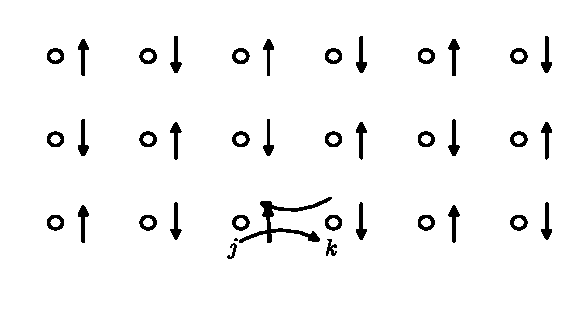
\includegraphics[width=0.6\textwidth]{fig_54.pdf}
\caption*{图 54　（原书图注仅作 “Figure 54”）交替自旋的子晶格阵列示意：三行格点各带向上、向下交替排列的自旋箭头；最下一行在格点 $j$、$k$ 处以弧形箭头画出一对正在交换的自旋}
\end{figure}
从铁磁的观点看，它含有非常高度的激发。然而正如我们所指出的，只要我们相信微扰论从 $n_\uparrow + n_\downarrow = 1$ 的准简并态流形出发是有效的、并且不允许向自由电子态作真实（有别于虚的）跃迁，这是完全没有问题的。

这样一种理论的有效性判据必须是：$b$ 应当比 $U$ 小得多。读者当还记得，在 Frenkel 激子情形中，当 $b$ 相对 $U$ 变大时，我们有一个从 Frenkel 型到 Wannier 型激子的快速的、但大概并非不连续的转变；而在这里，我们可以容易地看出，这个转变将是灾难性的。

正如同 Frenkel 激子的情形一样，关键问题围绕激子的结合能。然而在这里，我们并没有那个把电子从同一原子上的 $s$ 态激发到 $p$ 态所需的附加激发能 $E_0$；唯一阻止系统退化为纯粹金属态的能量，是电子与各自空穴之间的结合能。把电子从它的空穴中解放出来，我们可以获得量级为 $\sim Zb$ 的能量，但我们失去能量 $U$，而允许电子虚离开其空穴（以及相反的过程）所获得的只是二级能量 $-Zb^{2}/U$。于是我们可以估计 $Zb \sim U$ 作为从反铁磁体转变到金属的转变点的合理数值。此外，当 $b$ 大时，介电屏蔽再度成为问题，$U$ 自然也就更小。

处理向金属态转变这一问题的另一种、同样相当近似的方式，是问交替阵列究竟是不是多体问题的一个稳定的 Hartree 解。也就是说，我们可以问：$k$ 原子处自旋向下的电子所感受到的 Hartree 场相对于 $j$ 原子处的如何。名义上，这个差值是 $U$，即 $j$ 处自旋向上的电子与自旋向下的电子之间的排斥能。但在 Hartree 理论中，我们应当计及这样一个事实：$j$ 处的自旋向上电子并非时时刻刻都真正位于 $j$ 处，所以 Hartree 场的实际差值可能要小得多。

格点 $j$ 上的自旋向上电子以概率 $|b_{jk}/U|^{2}$ 跳到它的每一个近邻格点 $k$；同样，格点 $k$ 也可能以概率 $|b_{jk}/U|^{2}$ 被一个自旋向上电子占据。于是，$j$ 处的自旋向下态相对于 $k$ 处的自旋向下态的实际能量差为

\begin{align*}
\Delta E \;&=\; U\left(\langle n_{j\uparrow}\rangle - \langle n_{k\uparrow}\rangle\right) \\
&=\; U\left(1 - 2Z\,\Bigl|\frac{b_{jk}}{U}\Bigr|^{2}\right)
\end{align*}

但实际上，决定混杂大小的能量分母不应当是 $U$ 本身，而应当是 $\Delta E$，于是我们得到一个自洽方程

\begin{equation*}
\Delta E \;=\; U\left(1 - \frac{2}{(\Delta E)^{2}} \sum_{k} |b_{jk}|^{2}\right)
\end{equation*}

或

\begin{equation*}
(\Delta E)^{3} \;-\; U\,(\Delta E)^{2} \;=\; -\,2UZ\,|b_{jk}|^{2}
\end{equation*}

这个方程可以像图 55 所示那样图示出来。于是 $b$ 的最大可能值由下式给出：

\begin{equation*}
\left(\frac{b}{U}\right)_{\max} \;\cong\; \left(\frac{2}{27Z}\right)^{1/2} \;\sim\; \frac{1}{10}\ \text{左右}
\end{equation*}

在任一高于这个临界值的 $b$ 下，磁状态再也无法维持。它将对电子的重新分布不稳定：重新分布使两种自旋态的占据相等，态成为金属型的。铁系中较低的氧化物，

% ——上句在原书 p.163 末中断于 “The lower iron-series oxides,”，p.164（PDF p179）起由后续代理续译衔接。
以及后面几个过渡系列——V、Ru 等——的氧化物则是金属型的，尽管其中电子的迁移率相当低，只有通常金属中的 $10^{-3}$ 左右。有些氧化物表现出一种热致转变，有人提出，它也许在本质上是一种由金属型到磁性的转变 (9)。
\begin{figure}[H]
\centering
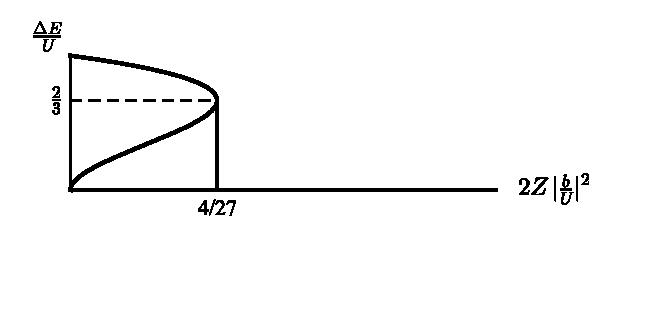
\includegraphics[width=0.72\textwidth]{fig_55.pdf}
\caption*{图 55　（原书图注仅作 “Figure 55”）p.163 自洽方程 $(\Delta E)^{3} - U(\Delta E)^{2} = -2UZ|b_{jk}|^{2}$ 的图解：纵轴为 $\Delta E/U$，横轴为 $2Z|b/U|^{2}$；曲线自原点出发，在虚线标出的 $\Delta E/U = 2/3$ 处达到极大，并于横坐标 $4/27$ 处陡降为零}
\end{figure}

\subsection{铁磁自旋波}

现在让我们继续讨论元激发（elementary excitations），先讨论铁磁情形 (96)。有效哈密顿量是

\begin{equation*}
\mathcal{H} = -\frac{1}{4} \sum_{jk} J_{jk}\, \boldsymbol{\sigma}_{j}\cdot\boldsymbol{\sigma}_{k}
\end{equation*}

（这里假定 $J_{jk} > 0$。）

自旋矢量与谐振子共有的一个最重要的性质是：它们的经典运动方程与量子运动方程完全相同。设 $\boldsymbol{\sigma}$ 与一个场 $\mathbf{H}$ 相乘后进入哈密顿量：$\mathcal{H} = -\frac{1}{2}\gamma\hbar\,\mathbf{H}\cdot\boldsymbol{\sigma}$。于是，当我们在 Heisenberg 表象中计算算符 $\boldsymbol{\sigma}$ 的运动方程时：

\begin{equation*}
i\hbar\,\frac{d\boldsymbol{\sigma}}{dt} = \left[\boldsymbol{\sigma},\, \mathcal{H}\right]
\end{equation*}

便得到

\begin{equation*}
i\hbar\,\frac{d\boldsymbol{\sigma}}{dt} = -\frac{\gamma\hbar}{2}\left[\boldsymbol{\sigma},\boldsymbol{\sigma}\right]\cdot\mathbf{H}
\end{equation*}

（这一记号的意思是：$[\boldsymbol{\sigma},\boldsymbol{\sigma}]$ 表示由分量 $[\sigma_{i},\sigma_{j}]$ 组成的并矢（dyadic）。）不同分量的对易子概括在关系式

\begin{equation*}
\boldsymbol{\sigma}\times\boldsymbol{\sigma} = 2i\boldsymbol{\sigma}
\end{equation*}

或者

\begin{equation*}
\sigma_{i}\sigma_{j} - \sigma_{j}\sigma_{i} = 2i\,\epsilon_{ijk}\,\sigma_{k}
\end{equation*}

之中，于是

\begin{equation*}
\left[\left[\boldsymbol{\sigma},\boldsymbol{\sigma}\right]\mathbf{H}\right]_{k} = 2i\sum_{j} H_{j}\,\epsilon_{kjl}\,\sigma_{l} = 2i\,\mathbf{H}\times\boldsymbol{\sigma}
\end{equation*}

因此

\begin{equation*}
\frac{d\boldsymbol{\sigma}}{dt} = \gamma\left(\boldsymbol{\sigma}\times\mathbf{H}\right)
\end{equation*}

这正是处于磁场 $\mathbf{H}$ 中、回磁比（gyromagnetic ratio）为 $\gamma$ 的自旋 $\mathbf{S} = \boldsymbol{\sigma}/2$ 的经典运动方程

\begin{equation*}
\frac{d\mathbf{S}}{dt} = \gamma\left(\mathbf{S}\times\mathbf{H}\right)
\end{equation*}

$\mathbf{H}$ 可以是一个 c 数（c-number），也可以是任何与所考虑的自旋 $\boldsymbol{\sigma}$ 对易的算符。

自旋 $\boldsymbol{\sigma}_{j}$ 所感受到的场 $\mathbf{H}$ 是 $\frac{1}{2\gamma\hbar}\sum_{k} J_{jk}\boldsymbol{\sigma}_{k}$。为方便起见，可以再附加一个小外场来引入一个优先方向 $\hat{\mathbf{z}}$，这在哈密顿量中导致一个 $\hbar\gamma H\sigma_{z}$ 项，于是我们便有运动方程

\begin{equation*}
\frac{d\boldsymbol{\sigma}_{j}}{dt} = \frac{1}{2\hbar}\sum_{k} J_{jk}\,\boldsymbol{\sigma}_{j}\times\boldsymbol{\sigma}_{k} + \gamma H\left(\boldsymbol{\sigma}_{j}\times\hat{\mathbf{z}}\right) \tag{24}
\end{equation*}

（译注：式 (24) 左端原书印作 $d\boldsymbol{\sigma}_{z}/dt$；按右端当为 $\boldsymbol{\sigma}_{j}$，此处径改。）

这些方程可以用来得到自旋波的运动方程，它们与用玻色子理论导出的方程完全等价；而且利用自旋和运动方程，许多性质可以直截了当地算出，根本不必经过赝玻色子近似（pseudo-boson approximation）。遗憾的是，热学的和能量的性质用这种方法却不那么容易处理，尽管近代的 Green 函数理论已在这个方向上取得了相当大的进展。尽管如此，记住下面这一点仍然十分重要：在自旋理论中，正如在谐振子理论中一样，大多数经典结果根本不是近似，而且人们的经典直觉可以具有极大的价值。

让我们把运动方程 (24) 明写出来：

\begin{align*}
\frac{d\sigma_{jx}}{dt} &= \frac{1}{2\hbar}\sum_{k} J_{jk}\left(\sigma_{jy}\sigma_{kz} - \sigma_{ky}\sigma_{jz}\right) + \gamma\sigma_{jy}H \\
\frac{d\sigma_{jy}}{dt} &= \frac{1}{2\hbar}\sum_{k} J_{jk}\left(\sigma_{jx}\sigma_{kz} - \sigma_{kx}\sigma_{jz}\right) - \gamma\sigma_{jx}H
\end{align*}

把第二式乘以 $-i$ 加到第一式上，我们得到

\begin{align*}
\frac{d\sigma^{-}_{j}}{dt} &= \frac{1}{2}\,\frac{d}{dt}\left(\sigma_{jx} - i\sigma_{jy}\right) \\
&= \frac{i}{2\hbar}\sum_{k} J_{jk}\left(\sigma^{-}_{j}\sigma_{kz} - \sigma^{-}_{k}\sigma_{jz}\right) + i\gamma\sigma^{-}_{j}H
\end{align*}

只有 $\sigma^{-}$ 出现这一事实表明，自旋波是圆偏振的。既然我们感兴趣的是把各种性质——热的与动力学的——都计算出来，那就让我们作玻色子变换

\begin{equation*}
\sigma^{-}_{j} = b^{\dagger}_{j}\left(1-n_{j}\right) \qquad\qquad \sigma_{jz} = 1 - 2n_{j}
\end{equation*}

我们把符号反了过来，原因是基态对应于 $\sigma_{z} = +1$，而一个自旋波所涉及的是把一个自旋转\emph{向下}。$b$ 的线性项是

\begin{equation*}
\frac{db^{\dagger}_{j}}{dt} = i\gamma H b^{\dagger}_{j} + \frac{i}{2\hbar}\sum_{k} J_{jk}\left(b^{\dagger}_{j} - b^{\dagger}_{k}\right)
\end{equation*}

当我们变换到自旋波变量 $\beta_{k}$ 时，我们得到

\begin{align*}
\frac{d\beta^{\dagger}_{k}}{dt} &= i\omega_{k}\beta^{\dagger}_{k} \\
\omega_{k} &= \gamma H + \frac{1}{2\hbar}\sum_{j} J_{0j}\left(1 - \cos\mathbf{k}\cdot\mathbf{j}\right) \tag{25}
\end{align*}

在没有磁场时，自旋波频率随 $k^{2}$ 从 $k=0$ 处的零值增大。除外场贡献之外频率在 $k=0$ 处必须为零，这一事实是下述恒等式的后果，该恒等式来自普遍的运动方程：

\begin{equation*}
\frac{d}{dt}\sum_{j}\sigma^{-}_{j} = \frac{i}{2\hbar}\sum_{jk} J_{jk}\left(\sigma^{-}_{j}\sigma_{kz} - \sigma^{-}_{k}\sigma_{jz}\right) \equiv 0
\end{equation*}

而且事实上，$S_{\mathrm{o}} = \sum_{j}\boldsymbol{\sigma}_{j}$，即总自旋矢量本身，是一个运动常数。$S^{-}$ 是 $k=0$ 自旋波算符的 $\sqrt{N}$ 倍。

这是我们第一次碰到集体激发的最重要普遍法则中的一条，它与哈密顿量中对称性的存在有关。交换哈密顿量 (23)，以及它所由之导出的原始哈密顿量，在自旋空间中的转动操作下不变。这是因为 Coulomb 相互作用和动能都不以任何方式涉及电子的自旋；自旋只是通过不相容原理、或者通过费米统计更完备的表述——对易关系——而进入问题。但对易关系本身在自旋转动（当然是同时转动所有自旋）之下也是不变的：

\begin{equation*}
\left[\Psi_{\sigma}(r),\ \Psi^{\dagger}_{\sigma}(r')\right] = \delta_{\sigma\sigma'}\,\delta(r-r')
\end{equation*}

在对应于自旋空间中一个转动的变换之后依然成立：

\begin{equation*}
\Psi_{+} \rightarrow \cos\frac{\theta}{2}\, e^{-i(\Phi/2)}\,\Psi^{'}_{+} + \sin\frac{\theta}{2}\, e^{i(\Phi/2)}\,\Psi^{'}_{-}
\end{equation*}

于是，当我们沿 $\theta,\Phi$ 方向而不是沿 $z$ 方向量子化时，$\Psi^{'}_{+}$ 就是波函数的 $+$ 分量（图 56）。
\begin{figure}[H]
\centering
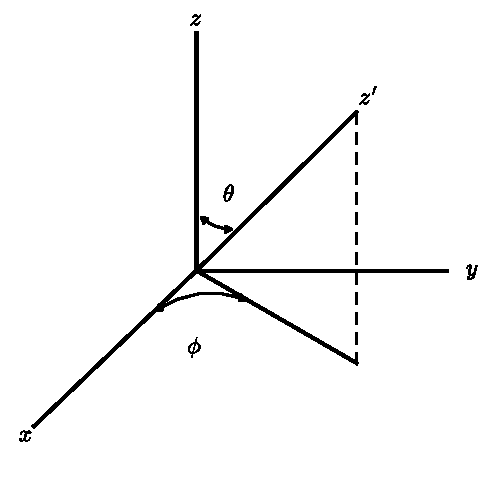
\includegraphics[width=0.72\textwidth]{fig_56.pdf}
\caption*{图 56　（原书图注仅作 “Figure 56”）坐标系示意图：$z'$ 轴相对 $z$ 轴的极角为 $\theta$，绕 $z$ 轴的方位角为 $\phi$}
\end{figure}

哈密顿量的每一个不变性都对应一个运动常数。对应于时间平移不变性，该常数是 $E$；对应于空间平移不变性，是 $\mathbf{P}$；对应于角向转动不变性，则是总角动量 $\mathbf{L}$。它们就是所谓的对称变换的“生成元”（generators）；例如，$L_{z} = i(\partial/\partial\Phi)$，而当 $\partial\mathcal{H}/\partial\Phi = 0$ 时，

\begin{equation*}
\frac{\partial}{\partial\Phi}\,\mathcal{H} - \mathcal{H}\,\frac{\partial}{\partial\Phi} = 0 \qquad \text{于是} \qquad \left[\mathcal{H},\ L_{z}\right] = 0
\end{equation*}

于是，自旋空间中的转动不变性意味着 $[\mathcal{H},\mathbf{S}] = 0$，即 $\mathbf{S} = \text{const.}$。实际上这并不是一个严格的对称性，因为电磁力中磁性的部分确实依赖于 $\boldsymbol{\sigma}$；它只在 $v/c \rightarrow 0$ 的极限下成立，因此，比如说，自旋-轨道耦合就破坏它。结果，真实的铁磁体具有所谓的“晶体各向异性能”（crystal anisotropy energy），它依赖于 $\mathbf{S}$ 在空间中的方向，但其大小几乎总是比交换能小得多——交换能来自 Coulomb 能，并且在基本上决定了磁性性质。

这一近似对称性保证了 $k=0$ 自旋波的频率应当接近于零。由 $k=0$ 自旋波的激发所得出的激发态是什么？原来的铁磁态恰好含有 $N$ 个电子，每个都处于自旋朝上的态，因此总自旋为 $S = N/2$（$\sigma_{\mathrm{tot}} = N$），精确地指向 $z$ 方向。由于哈密顿量的转动不变性，$z$ 方向当然是完全任意的；我们当初未尝不可以沿 $x$ 或 $y$ 方向、或沿任何其他方向量子化，只要我们愿意。与此相应，基态存在简并；坚持取 $z$ 为量子化方向，我们本可以选

\begin{equation*}
S_{z} = -\frac{N}{2},\ -\frac{N}{2} + 1,\ \cdots,\ 0,\ 1,\ \cdots,\ \frac{N}{2} - 1,\ \frac{N}{2}
\end{equation*}

而这些严格本征态中的每一个都与原来的态具有完全相同的能量。对这些态取适当的线性组合，我们就可以构成一个 $S_{z'} = N/2$ 的态，其 $z'$ 指向任意方向 $\theta,\Phi$。应当取什么样的线性组合，可以由相应的表示系数 $D^{N/2}_{N/2,\,N/2}(\theta,\Phi)$ 算出；或者用这样一个技巧：把（这 $N$ 个电子的）态看作由乘积

\begin{equation*}
\alpha(1)\,\alpha(2)\cdots\alpha(N)
\end{equation*}

构成［$\alpha(i)$ 是与 $\sigma_{j}$ 相对应的波函数的自旋朝上分量］，并利用变换

\begin{equation*}
\alpha \rightarrow \alpha^{'}\cos\frac{\theta}{2}\, e^{i(\Phi/2)} + \beta^{'}\sin\frac{\theta}{2}\, e^{-i(\Phi/2)}
\end{equation*}

显然，从 $S_{z} = N/2$、$S = N/2$ 的态出发，逐次激发 $k=0$ 自旋波所得到的态，是 $S = N/2$ 但 $S_{z} = (N/2) - 1$、$(N/2) - 2$ 等等的态。这是因为

\begin{equation*}
\beta^{\dagger}_{k=0} = \frac{1}{\sqrt{N}}\sum_{j}\sigma^{-}_{j} = \frac{1}{\sqrt{N}}\,S^{-}
\end{equation*}

而 $S^{-}$ 就是“下降算符”（lowering operator），它使 $S_{z}$ 减小一个单位而不改变 $|S|$。这样我们看到，基态的转动不变性与 $k=0$ 模的零频率是等价的。

即使存在磁场，由 $k=0$ 模激发所到达的本征态仍是同样的这些态，因为在微扰 $\hbar\gamma H S_{z}$ 之下 $S_{z}$ 和 $|S|$ 仍然是好量子数。这时 $k=0$ 自旋波的频率不是零而恰好是 $\gamma H$。注意，关于均匀模频率的这些论断，在不存在自旋-轨道力的前提下，对哈密顿量的所有态都成立；这是显而易见的，因为 $S^{-}$ 的作用不过是把任何一个态转动一下。这就是那条著名的定理：“单是交换并不会展宽磁共振频率。”换一种说法：$k=0$ 自旋波与 $k\neq 0$ 的自旋波不以任何方式发生相互作用。

那么，$k\neq 0$ 的自旋波又如何？有一个显而易见的假设（而且事实证明确实如此）：当只考虑交换力时，自旋波的频率将连续地衔接到 $k=0$ 模的频率——也就是说，当 $k \rightarrow 0$ 时 $\omega \rightarrow 0$。

鉴于 $k \rightarrow 0$ 极限在其他问题中的种种复杂性，这一点并非显而易见，它是交换力短程性质的一个结果。例如，当我们把长程磁偶极力计入时，$k=0$ 模的频率就要依赖于样品的形状，因为表面磁极引起的退磁效应依赖于样品形状。而且纵向与横向自旋波的频率各不相同，所以当 $k \rightarrow 0$ 时根本谈不上连续性。与此相反，交换力基本上是短程的，因为除去磁偶极效应和自旋-轨道效应之外，自旋矩的重新分布在长距离上不会以任何可察觉的方式影响电荷分布。

这就是我想强调的重要联系，因为它在集体激发和相变的普遍理论中起着至关重要的作用。我们从一个哈密顿量

\begin{equation*}
\frac{1}{4} \sum_{jk} J_{jk}\,\boldsymbol{\sigma}_{j}\cdot\boldsymbol{\sigma}_{k}
\end{equation*}

（译注：此式原书未印负号；对照本节开头 $\mathcal{H} = -\frac{1}{4}\sum_{jk}J_{jk}\boldsymbol{\sigma}_{j}\cdot\boldsymbol{\sigma}_{k}$，疑为漏印，照录原书。）

出发，它在自旋空间中具有完全的转动对称性。尽管有这种转动对称性，我们所假定的那个最低本征态——它在某些特殊条件下、即所有 $J_{jk} < 0$ 时\emph{确}实是最低本征态——却并不具有完全的转动对称性。只有单态（$S_{\mathrm{tot}} = 0$）才具有。因此，最低本征态必定与大量其他态简并：这些态指向不同的方向，或者（如果我们愿意这样看）沿同一方向具有不同的 $S_{z}$。

于是我们得出结论：至少存在一种形式的元激发，即对应于 $k=0$ 的那一种，它给出整个系统在自旋空间中的一个转动，并且其频率必为 $\omega = 0$。在再加一条物理条件——不存在长程力——之下，这就意味着元激发能谱中有整整一支，当 $k \rightarrow 0$ 时 $\omega \rightarrow 0$。

如今，自旋波已经成为一种和声子同样实实在在的实验现象。人们已用中子非弹性散射、用薄膜中磁共振的直接观测、用与声子谱的耦合以及若干其他较为间接的方法对它进行过研究。不过，它最为人熟知的性质，是它对磁化强度和比热的温度依赖关系的影响。频率为 $\hbar\omega = Ak^{2}$ 的一支玻色型激发具有数密度

\begin{equation*}
N = 4\pi\int_{0}^{k_{\max}} \frac{k^{2}\,dk}{e^{\beta Ak^{2}} - 1} \qquad\qquad \beta = \frac{1}{k_{\mathrm{B}}T}
\end{equation*}

而当 $Ak_{\max}^{2} \gg k_{\mathrm{B}}T$ 时——即在低温下——这显然变为

\begin{align*}
N \approx 4\pi\int_{0}^{\infty} \frac{k^{2}\,dk}{e^{\beta Ak^{2}} - 1} &= \frac{4\pi}{(\beta A)^{3/2}}\int_{0}^{\infty} \frac{x^{2}\,dx}{e^{x} - 1} \\
&= \frac{4\pi\,(k_{\mathrm{B}}T)^{3/2}}{A^{3/2}} \times \text{const.}
\end{align*}

现在我们注意到，每个自旋波所对应的反转自旋数恰好是 1，因此 $S_{z}$ 的改变就正比于 $T^{3/2}$——这正是 Bloch 理论中著名的温度变化关系。Dyson (81) 已对这一变化关系计算了修正项：来自对 $\hbar\omega = Ak^{2}$ 的偏离的有 $T^{5/2}$ 和 $T^{7/2}$ 项，而第一个自旋波相互作用项则是 $T^{4}$ 量级的项，完全可以忽略。我们起初也许会以为 $A(T) \propto \text{const.} - N$，从而预期有一个 $T^{3}$ 项；但是长波长自旋波之间的相互作用非常小，其原因基本上是与 $k=0$ 波的连续衔接——后者与其他自旋波没有任何相互作用。人们发现

\begin{equation*}
\omega \propto k^{2}\left[\text{const.} - \int \left[k'^{2}N(k')\right] k'^{2}dk'\right] \propto k^{2}\left[\text{const.} - T^{5/2}\right]
\end{equation*}

其中 $N(k)$ 是波矢为 $\mathbf{k}$ 的自旋波的平均数目。相应地，修正项就是 $T^{3/2}T^{5/2} = T^{4}$。自旋波比热同样 $\propto T^{3/2}$：能量为

\begin{equation*}
U = 4\pi A\int \frac{k^{2}}{e^{\beta Ak^{2}} - 1}\, k^{2}dk \propto T^{5/2} \qquad\qquad C = \frac{\partial U}{\partial T} \propto T^{3/2}
\end{equation*}

这些积分在 $k=0$ 附近的行为说明了一个重要的论点。在任一有限温度下、靠近 $k=0$ 处，自旋波密度 $N(k)$ 就是经典值

\begin{equation*}
N(k) = \frac{k_{\mathrm{B}}T}{\hbar\omega(k)} = \frac{k_{\mathrm{B}}T}{Ak^{2}}
\end{equation*}

请注意，假如系统只有两维，从而态密度 $\propto k\,dk$，那么磁化偏离的积分将在 $k \rightarrow 0$ 处对数发散。不过，任何小的外场或自旋-轨道耦合都可以使 $k=0$ 自旋波的频率变为有限，从而使积分收敛，其形式大致为

\begin{equation*}
T\ln\left(\frac{k_{\mathrm{B}}T}{\text{截断能量}}\right)
\end{equation*}

这种二维发散也是具有短程力的有序系统的一个非常普遍的性质。例如，人们相信，如果没有某种有序的支撑，二维晶体将不是热力学稳定的。然而，对于二维情形不存在相变这一点，看来实际上并没有证明 (98)。

现在我想把这些结果与两种不同类型的经典理论的结果联系起来。第一种是纯经典自旋矢量所对应的同一个问题。假定代替 Pauli 自旋算符 $\boldsymbol{\sigma}_{j}$，我们有的是经典自旋矢量 $\mathbf{S}_{j}$：

\begin{equation*}
\mathcal{H} = -\sum_{jk} J_{jk}\,\mathbf{S}_{j}\cdot\mathbf{S}_{k}
\end{equation*}

我们定义 $\mathbf{S}_{j} = \mathbf{J}_{j}/\hbar$，其中 $\mathbf{J}_{j}$ 是真实的经典角动量。这样，经典交换参量便是 $J_{jk}/\hbar^{2}$。我们指出这一点，是因为我们人为地使用 $\mathbf{S}$ 而不是 $\mathbf{J}$，可能会在实际上是经典的方程中引进 $\hbar$ 因子。

这个哈密顿量的最低态，应当是所有经典自旋矢量都完全沿同一方向排列的态。我们可以把这一能量在平衡位置附近展开，从而用这种阵列的经典进动模导出一个近似哈密顿量：

\begin{equation*}
\mathbf{S}_{j}\cdot\mathbf{S}_{k} = S_{zj}S_{zk} + S_{xj}S_{xk} + S_{yj}S_{yk}
\end{equation*}

\begin{equation*}
S_{zj}^{2} = S^{2} - S_{xj}^{2} - S_{yj}^{2}
\end{equation*}

于是

\begin{equation*}
S_{zj} \simeq S - \frac{1}{2S}\left(S_{xj}^{2} + S_{yj}^{2}\right)
\end{equation*}

因为在平衡位置附近第二项很小。这样便有

\begin{align*}
-\mathcal{H} &= -NZJS^{2} + \sum_{jk} J\left[\left(S_{xj} - S_{xk}\right)^{2} + \left(S_{yj} - S_{yk}\right)^{2}\right] \\
&= -NZJS^{2} + \sum_{\substack{jk \\ \text{近邻}}} \frac{J}{2}\left[\left(S^{+}_{j} - S^{+}_{k}\right)\left(S^{-}_{j} - S^{-}_{k}\right) + \left(S^{-}_{j} - S^{-}_{k}\right)\left(S^{+}_{j} - S^{+}_{k}\right)\right]
\end{align*}

（译注：首行左端原书印作 $-\mathcal{H}$；按上页 $\mathcal{H} = -\sum_{jk}J_{jk}\mathbf{S}_{j}\cdot\mathbf{S}_{k}$ 推算当为 $\mathcal{H}$，与下文式 (26) 对照亦可见负号为误印，照录原书。）

这里我们假定了 $J_{jk}$ 除原子与其 $Z$ 个近邻之间外处处为零，这是一种非本质的简化。$S^{-}$ 与 $S^{+}$ 的定义与量子力学自旋的情形相同。我们还可以再前进一步，注意到无论经典地还是量子力学地，自旋的小振荡 $\hbar^{1/2}(\delta S_{x}/\sqrt{S})$ 与 $\hbar^{1/2}(\delta S_{y}/\sqrt{S})$ 都服从正则共轭变量的 Poisson 括号关系。更简单地说，我们指出，自旋的经典运动方程与量子运动方程是等同的，因此系统的经典模同样是进动波：

\begin{equation*}
S^{-}_{j}(t) = e^{i\omega_{\lambda} t}\, e^{i\boldsymbol{\lambda}\cdot\mathbf{j}}
\end{equation*}

也就是说，我们可以导出一组简正模（normal modes）

\begin{align*}
S^{-}_{\lambda} &= \frac{1}{\sqrt{NS}}\sum_{j} e^{i\boldsymbol{\lambda}\cdot\mathbf{j}}\, S^{-}_{j} \\
S^{-}_{\lambda} &\propto e^{i\omega_{\lambda} t}
\end{align*}

$\omega_{\lambda}$ 由下式给出：

\begin{equation*}
\omega_{\lambda} = \frac{S}{\hbar}\sum_{j} J_{0j}\left(1 - \cos\boldsymbol{\lambda}\cdot\mathbf{j}\right)
\end{equation*}

若在 (25) 中代入 $S = 1/2$，此式便与 (25) 相一致；而如果我们代入 $J = \hbar S$，并意识到 $J_{0j}$ 是经典交换参量的 $\hbar^{2}$ 倍，它也还是一个纯经典的公式。哈密顿量约化为

\begin{equation*}
\mathcal{H} = -NZJS^{2} + \sum_{\lambda} \frac{\omega_{\lambda}}{2}\left(S^{+}_{\lambda}S^{-}_{\lambda} + S^{-}_{\lambda}S^{+}_{\lambda}\right) \tag{26}
\end{equation*}

当然，经典地看次序无关紧要；但当我们把系统量子化时，就必须像通常那样选取这个对称化了的厄米组合。

关于零点运动和零点能量的情形起初是令人困惑的。量化的经典 Hamilton 量与相应的量子结果之间好像有出入，因为量子力学中基态能量恰好是 $-NZJS^{2}$，这里没有为对易子项带来的修正留有余地——这一修正必定来自把 $S^{+}S^{-} + S^{-}S^{+}$ 项重新编序并加以修正：

\begin{align*}
\frac{1}{2}&\left\{\left(S^{x}_{\lambda} + iS^{j}_{\lambda}\right)\left(S^{x}_{\lambda} - iS^{y}_{\lambda}\right) - \left(S^{x}_{\lambda} - iS^{y}_{\lambda}\right)\left(S^{x}_{\lambda} + iS^{y}_{\lambda}\right)\right\} \\
&= -i\left(S^{x}_{\lambda}S^{y}_{\lambda} - S^{y}_{\lambda}S^{x}_{\lambda}\right) = i\frac{1}{NS}\sum_{j} iS^{z}_{j} \\
&= 1
\end{align*}

（译注：照录原书。首行第一个括号中的 $S^{j}_{\lambda}$ 显系 $S^{y}_{\lambda}$ 之误。又，按对易关系 $[S^{x},S^{y}] = iS^{z}$，第二行左端 $-i(S^{x}_{\lambda}S^{y}_{\lambda} - S^{y}_{\lambda}S^{x}_{\lambda})$ 应等于 $\frac{1}{NS}\sum_{j} S^{z}_{j}$（基态中 $\sum_{j}S^{z}_{j} = NS$），故该行系数中的两个 $i$ 多出一个，否则与末行 “$= 1$” 不相容。）

Klein 与 Smith (99) 最先指出，情况之所以得救，是由于与量子自旋矢量 $\mathbf{S}$ 相对应的经典自旋是 $S^{'} = \sqrt{S(S+1)}$，也就是说，$S(S+1) = S_{xj}^{2} + S_{yj}^{2} + S_{zj}^{2}$。于是，$S_{zj}^{2} = S^{2} - (S_{xj}^{2} + S_{yj}^{2} - S)$；再次应用近似对易关系

\begin{equation*}
S_{xj}S_{yj} - S_{yj}S_{xj} = iS_{zj} \simeq iS
\end{equation*}

就得到

\begin{align*}
S_{zj}^{2} &= S^{2} - \left[\frac{1}{2}\left(S^{+}_{j}S^{-}_{j} + S^{-}_{j}S^{+}_{j}\right) - S\right] \\
&\simeq S^{2} - S^{-}S^{+}
\end{align*}

因此，只有把 $S^{2}$ 改成 $S(S+1)$，(26) 才是正确的对应原理哈密顿量；而这样一改，它便与量子结果完全一致：

\begin{equation*}
\mathcal{H} = -NZJS^{2} + \sum_{\lambda} \omega_{\lambda}\, S^{-}_{\lambda}S^{+}_{\lambda}
\end{equation*}

其结果是经典理论与量子理论之间的完全对应。同激子情形中我们略去“逆向图”（backward diagrams）时一样，零点运动效应不过是一种相当平凡的数学练习，只与单个原子的内部动力学有关；耦合项的零点平均值净效果为零，因为零点效应要对所有自旋波 $\lambda$ 求和，而 $\sum_{\lambda}\cos\lambda = 0$（在这里，$\cos\lambda$ 就是耦合项的 Fourier 变换）。

还有第二种用途非常普遍的处理磁性问题的半经典方法，它是由 Landau、Lifshitz、Kittel 与 Herring (100) 提出的。这一方法非常接近于声子的 Debye 理论。其想法是立足于相当粗粒的观点，把磁化强度看作一个连续的磁化场 $\mathbf{M}(r)$，它服从连续量子场的对易关系

\begin{equation*}
\mathbf{M}(r)\times\mathbf{M}(r') = i\mathbf{M}(r)\,\delta(r-r')\ \left(\times\ \text{consts.}\right)
\end{equation*}

哈密顿量依赖于 $(S_{j} - S_{k})^{2}$ 这一形式提示我们，作为半经验的哈密顿量密度可以取

\begin{equation*}
\mathcal{H} = A\int dr\left(\nabla\mathbf{M}(r)\right)^{2} \tag{27}
\end{equation*}

可以证明，对绝缘铁磁体这一特殊情形它是正确的；而且显而易见，它也是任何短程、各向同性的力的宏观必然后果——正如弹性理论必然给出一个形变 $(\nabla u)$ 的二次型哈密顿量一样（$u$ 为位移）。由此导出了普遍的磁化运动方程，人们可以猜想，它们在所有铁磁体中都成立：

\begin{equation*}
\frac{d\mathbf{M}}{dt} = A\left(\mathbf{M}\times\nabla^{2}\mathbf{M}\right) + \gamma\left(\mathbf{M}\times\mathbf{H}_{\mathrm{ext}}\right) + \left(\text{耗散项}\right)
\end{equation*}

这就是 Landau-Lifshitz 方程，它在所有自旋波理论和铁磁共振理论中都起着基础性的作用。

像 (27) 这样的哈密顿量——以及弹性理论中相应的哈密顿量

\begin{equation*}
\mathcal{H} = \int \nabla\mathbf{u}:\mathbf{C}:\nabla\mathbf{u} \qquad \left(\mathbf{C}\ \text{为刚度弹性张量}\right)
\end{equation*}

——所共有的一个有趣性质，就是下述普遍论证：具有短程力的二维系统不可能有稳定的长程序。我们很容易相信，系统的长波长运动——至少当其频率很低时——在任一有限温度下都按经典方式行为。于是按能量均分，每个自由度 $k$ 分得 $k_{\mathrm{B}}T$ 的能量，而能量是

\begin{equation*}
\propto k^{2}\left(\nabla\mathbf{M}(k)\right)^{2} \qquad \text{故} \qquad \left\langle\left(\nabla\mathbf{M}(k)\right)^{2}\right\rangle = \frac{k_{\mathrm{B}}T}{k^{2}}
\end{equation*}

于是涨落积分

\begin{equation*}
\left\langle\Delta M^{2}\right\rangle = \int k^{D-1}\,dk\,\frac{k_{\mathrm{B}}T}{k^{2}} \qquad \left(D\ \text{为维数}\right)
\end{equation*}

在磁性与弹性两种情形中都在 $D = 2$ 时发散。换一种说法就是：在二维情形下，人们可以在样品中的任何地方造就一个尺寸为 $\sim 1$ 的反向磁畴，四周由厚度 $\sim 1$ 的“Bloch 墙”所包围，其能量为（墙中原子数）$\times\,(\nabla M)^2 \sim 1^2(1/1^2)M^2 =$ 有限值。于是，在样品的所有区域内、在任意尺度上、并且以实质上无限多种可能的组态，这类磁畴都具有一份有限的热激发概率。这样，长程序便被破坏了。一般说来，只要变化缓慢，Landau-Lifshitz 方程使我们能够处理比自旋波更复杂、更一般的运动与组态。

\subsection{反铁磁自旋波与“对称破缺”}

最后，我要对反铁磁自旋波（antiferromagnetic spin waves）这一课题 (101) 作一简短的介绍。它们之所以重要，是因为在零点运动、对称性与元激发谱之间的种种关系中，它们大概是我们能归并在“对称破缺理论”（theory of broken symmetry）名下的各种情形中最简单、也理解得最好的一例；而这些关系在几乎所有形式的量子凝聚——固体与声子、自旋波、超导电性、液氦以及等离体——的理论中都起着至关重要的作用。

一般说来，凝聚现象的特征是：在我们称为“凝聚”系统的状态中出现了一个原先系统中不存在的新参量。铁磁体在 Curie 点以上、没有外场时没有磁化；在 Curie 点以下则有。在反铁磁体中，新参量便是反铁磁序。例如，我们可以取两个子晶格磁化之差作为参量——它常被称为“序参量”（order parameter）。合金中的有序-无序有一个明显的新参量，铁电性也是如此。同样明显的是固体的长程序，它在液体中并不存在。液氦 II 有一个参量，如今普遍理解为处于零动量态中的原子数。液-气系统则更难以捉摸一些，但利用所谓“格气”（lattice gas）方法，我们可以把它类比于一个经典的有序-无序系统。更加难以捉摸、然而却完全类似的，是超导体的序参量，它可以定义为与能隙相联系的某个非对角的“Green 函数”。

所有这些序参量都有一个共同的特点：当序参量出现时，系统比起未凝聚相来具有较低的对称性。这一点在多数情形下又是十分明显的，尽管对两种超流体而言，这种较低的对称性是相当特殊而且有争议的一种，即通常意义下规范不变性的缺失（也许更为普遍接受的观点是零动量起着特殊作用，即缺乏 Newton 不变性）。在多数其他情形中，对称性的改变属于那种对一般理论物理学家的敏感神经刺激较小的一类，因为他更熟悉那些破坏对称性的微扰的存在。这样，理想的铁磁体与反铁磁体都已抛弃了自旋空间中交换力的转动对称性——这种对称性反正会被磁性微扰所破坏。铁磁态与反铁磁态不具有时间反演对称这一事实（对铁磁体而言这是一件非常实际的事，因为它使铁氧体回转器得以存在）本应几乎同超导体中的规范（不变性）一样使理论家感到不安，因为时间反演通常被认为是一种严格成立的对称性。固体已经抛弃了完全的转动对称性与平移对称性，这同样不会扰乱我们的直觉，但这仅仅是因为我们天天都在同固态的夹具和匣子打交道，而它们恰好具有同样奇特的对称性缺失。尽管如此，在所有这些情形中，我们通常都取一个\emph{具有}适当对称性的哈密顿量表达式，然后我们从它导出——或者假定我们能够导出——系统的一个态，该态由这个哈密顿量决定，但却\emph{不具有}这种对称性。这样看来，据我所见，这正是一切凝聚现象的一个普遍特征。

在所有这些凝聚相之中，铁磁性是独一无二的，或者差不多是独一无二的：在这种情形中，序参量至少近似地是一个\emph{运动常量}（constant of the motion）。这一事实使我们能够作极大的简化。首先，在纯铁磁体的理想化 Heisenberg 模型中，我们能够写下系统的一个精确基态；在更复杂的模型中，例如 Heisenberg 亚铁磁体，我们至少能够用一个好量子数——总自旋，和/或其总的 $z$ 分量——来表征基态。这样一个好量子数的存在，意味着关于基态对称性的一个严格论断。于是我们可以这样表征所有激发态：其中至少有一个被反转的自旋。这种情况就像 $N+1$ 体问题中的情形一样：带有元激发的态确实能够同基态清楚地分辨开来。而且，磁化反转的数量也同粒子数的改变一样，是每个元激发的一个固定常量。我们在前面已经指出，哈密顿量中在铁磁态被“破坏”的那个对称性的存在，当然意味着实际上存在着一整族基态——在此时此地为 $N+1$ 个——它们通过整个自旋系统的转动而相互变换。由于自旋是运动常量，这些不同的态都是哈密顿量的精确本征态，而且正如我们已看到的，这意味着 $\omega(k{=}0)$ 恒等于零。

在几乎所有其他有趣的凝聚情形中，序参量都不是运动常量。让我们以最简单的情形——反铁磁性——为例。一种特别简单的理想反铁磁体的哈密顿量是

\begin{equation*}
\mathcal{H} \;=\; J\sum_{jl} \mathbf{S}_j\cdot\mathbf{S}_l
\end{equation*}

其中我们不妨作一些非实质性的简化：设各个 $\mathbf{S}$ 位于一个简单立方晶格上，而 $J$ 只在最近邻之间起作用，于是 $\mathbf{S}_j$ 总可以取在面心立方子晶格 A 上，而 $\mathbf{S}_l$ 在 B 上（图 57）。
\begin{figure}[H]
\centering
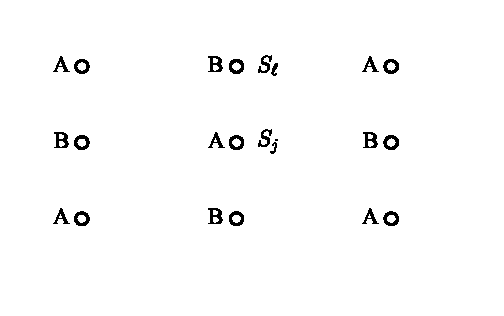
\includegraphics[width=0.72\textwidth]{fig_57.pdf}
\caption*{图 57　（原书图注仅作 “Figure 57”）简单立方晶格的 3×3 格点阵列：中心格点属 A 子晶格，其自旋标为 $\mathbf{S}_j$；上、下、左、右四个近邻格点属 B 子晶格，其一标出自旋 $\mathbf{S}_l$；四角格点亦属 A 子晶格}
\end{figure}

A 子晶格自旋的运动方程是

\begin{align*}
\bigl[\mathcal{H},\ \mathbf{S}_A\bigr] \;&=\; J\sum_j \mathbf{S}_j \times \sum_{\text{neighbors to j}} \mathbf{S}_l \\
&=\; J\sum_{\text{nearest-neighbor pairs}} \mathbf{S}_j \times \mathbf{S}_l \;=\; -\bigl[\mathcal{H},\ \mathbf{S}_B\bigr]
\end{align*}

其中 $\mathbf{S}_B$ 是另一子晶格的总自旋。于是，尽管总自旋 $\mathbf{S}_A + \mathbf{S}_B$ 按我们的一般定理是运动常量，但自旋之差 $\mathbf{S}_A - \mathbf{S}_B$ 的任何一个分量却都不是：

\begin{equation*}
\bigl[\mathcal{H},\ \mathbf{S}_A - \mathbf{S}_B\bigr] \;=\; 2J\sum_{\text{pairs}} \mathbf{S}_j \times \mathbf{S}_l
\end{equation*}

右端这个量，在系统邻近反铁磁态的任何可能态中都断然不为零；在铁磁态中它则可以为零。例如，它的（−）分量为

\begin{equation*}
\bigl[\mathcal{H},\ \mathbf{S}_A^- - \mathbf{S}_B^-\bigr] \;=\; J\sum_{j,l} \left(S_j^- S_{lz} - S_l^- S_{jz}\right)
\end{equation*}

在 $S_{jz} = S$、$S_{lz} = -S$ 的态（它决不是一个本征态）中，它就是

\begin{equation*}
\frac{JS}{\hbar}\sum_{jl}\left(S_j^- + S_l^-\right)
\end{equation*}

其矩阵元在该态中并不为零，尽管当然不存在\emph{对角}元。一般说来，我不作冗长的论证，只向读者保证：在反铁磁情形，$\mathbf{S}_A - \mathbf{S}_B$ 不可能是运动常量。

另一方面，毫无疑问确实发生的是：这个“序参量”变量的进动速率可以极其缓慢——在系统尺寸趋于无限的极限下，缓慢到可以忽略。

让我们取严格的运动方程

\begin{equation*}
i\hbar\,\frac{d}{dt}\left(\mathbf{S}_A - \mathbf{S}_B\right) \;=\; 2J\sum_{\text{pairs}}\left[\mathbf{S}_j \times \mathbf{S}_l\right]
\end{equation*}

两个子晶格的平均自旋 $\mathbf{S}_A$ 与 $\mathbf{S}_B$ 是非常多个原子的自旋之和，因而颇像经典变量，诸如宏观物体的位置与动量；它们的不确定度只需具有相对量级 $N^{-1/2}$。如果我们假定 $\mathbf{S}_A$ 与 $\mathbf{S}_B$ 确实具有某种宏观平均值，那么按对称性，量 $\mathbf{S}_j$ 与 $\mathbf{S}_l$ 的平均值——虽然不是它们的非对角矩阵元，即量子涨落——看来应当由下式给出

\begin{equation*}
\langle \mathbf{S}_j\rangle \;=\; \frac{\langle \mathbf{S}_A\rangle}{N}\,,\qquad \langle \mathbf{S}_l\rangle \;=\; \frac{\langle \mathbf{S}_B\rangle}{N}
\end{equation*}

于是，代入各变量的\emph{平均值}（average values），我们可以写出一个 c 数（c-number）运动方程

\begin{equation*}
i\hbar\,\frac{d}{dt}\langle \mathbf{S}_A - \mathbf{S}_B\rangle \;=\; \frac{2JZ}{N}\,\langle \mathbf{S}_A\rangle \times \langle \mathbf{S}_B\rangle
\end{equation*}

取 $\langle \mathbf{S}_A\rangle = -\langle \mathbf{S}_B\rangle$——这显然是平均能量最低的态——右端便变为零，而且至少在 $N$ 的量级上，序参量 $\langle \mathbf{S}_A\rangle - \langle \mathbf{S}_B\rangle$ 成为常量。当然，我们在这个方程右端略去了量子涨落，但我们可以假设，相对于任何 $\sim N$ 个元素之和的平均值，涨落具有 $1/\sqrt{N}$ 的量级。这完全不是一个严格的证明，但足以指示事情的走向。

另一方面，由于 $\mathbf{S}_A - \mathbf{S}_B$ 并非真正的运动常量，它的值必定要涨落。事实上，涨落必定具有 $N$ 的量级。Hulthen (103) 曾证明，对任何具有 $\mathcal{H} = J\sum_{\text{n.n.}}\mathbf{S}_j\cdot\mathbf{S}_l$（若 $J>0$）的有限系统，其真实的精确基态必有 $S_{\text{tot}} = \mathbf{S}_A + \mathbf{S}_B = 0$。这在物理上其实是显而易见的。但在 $S_{\text{tot}} = 0$ 的态中，$\langle \mathbf{S}_A\rangle = \langle \mathbf{S}_B\rangle = 0$，因为这样的态是完全各向同性的。（这是一个严格的群论结果。）

这看起来是一个颇为令人困惑的悖论。观测以及一种推理方式告诉我们 $\langle \mathbf{S}_A\rangle = -\langle \mathbf{S}_B\rangle \sim N$，而且这种情形不随时间发生宏观变化；另一种基于对称性的推理则说 $\langle \mathbf{S}_A\rangle = \langle \mathbf{S}_B\rangle = 0$。答案在于：后者在\emph{精确基态}（exact ground state）中是正确的，但这个精确的态无关紧要，因为许多别的态与它相距无穷小（能量上约 $1/N$）。因此，如果我们取 $\langle \mathbf{S}_A\rangle = -\langle \mathbf{S}_B\rangle \sim N$ 的态作为我们的态，它将维持非常长的时间，但由于它实际上是一个由许多精确态组成的波包，最终将会解体。

这与一个宏观固体在自由空间中的行为之间，存在着非常贴切而且精确的类似。这样的物体有一个质心坐标 $Q$、一个相应的动量 $P$，以及一个哈密顿量 $P^2/2MN$，$N$ 为粒子数。$P=0$ 将是精确的基态，此时 $Q$ 将剧烈地涨落：$Q$ 不可能是运动常量。事实上，当 $P\to 0$ 时 $\langle Q^2\rangle\to\infty$。但是各能级彼此靠得极近，因此，如果我们想把整个物体定域在一段非常小的距离之内——比如一个晶格常数的量级，$\Delta Q\sim 1$——相应的 $P$ 的增加为 $\sim 1$，$E$ 的增加为 $\sim 1/N$。于是这些能级是如此接近简并，以至于为了实用的目的——例如为了研究固体的内部结构——我们可以把 $\langle Q\rangle$ 固定下来，然后在 $\langle Q\rangle$ 从其预设值明显涨落之前去研究内部的自由度。或许一个更直接的例子，是宏观刚性旋转体的取向 $\theta$ 与角动量 $I\omega$。

但是我们必须认识到两点：其一，使 $Q$ 或 $\mathbf{S}_A - \mathbf{S}_B$ 的一切取值彼此等价的那个对称性的存在，使这个变量的宏观运动频率为零。这正好就是我们在铁磁性中关于序参量 $\mathbf{S}$ 所得到的结果，尽管在我们的情形中序参量并不是运动常量。其二，这个参量的\emph{涨落}必须为无穷大，这一事实带来了另一个结果。在短程力的情形，宏观能量只能依赖于序参量的\emph{梯度}：

\begin{equation*}
U \;\propto\; \bigl|\nabla\left(\mathbf{S}_A - \mathbf{S}_B\right)\bigr|^2 \qquad\text{或}\qquad \bigl|\nabla Q\bigr|^2
\end{equation*}

但这将意味着

\begin{equation*}
\Bigl\langle\bigl|\nabla(\mathbf{S}_A - \mathbf{S}_B)\bigr|^2\Bigr\rangle \;=\; k^2\langle S_k^2\rangle \;\propto\; \langle V\rangle \;=\; \frac{\hbar\omega_k}{2}
\end{equation*}

于是

\begin{equation*}
\langle S_k^2\rangle \;=\; \frac{\omega_k}{k^2} \;\to\; \infty \qquad\text{当 } k\to 0
\end{equation*}

因此我们预期 $\omega_k\to 0$，但 $\omega_k/k^2\to\infty$。实际上，在最广为人知的那些情形（反铁磁性、固体与液体中的声子）中，$\omega_k\propto k$。核物质的表面振荡 (104) 则有 $\omega_k\propto k^{3/2}$。

当存在低频模式时，与这类凝聚总是相伴随的最后一个效应，是一种长程力。长程力同零质量（即当 $k\to 0$ 时 $\omega\to 0$）粒子之间不可避免的关联，我在这里没有时间详细讨论，只打算提及两个最著名的例子：一是经由铁磁或反铁磁矩的极化而起作用的 Suhl-deGennes 长程核自旋-自旋相互作用 (105)；其二自然是人所共知的、围绕点源的弹性形变的长程性质，它使晶体中空位等的弹性相互作用仅按 $1/r$ 衰减。

现在，我简略地给出反铁磁自旋波的数学处理。附带说一句，这里关于自旋波与磁性的许多材料，都载于我发表在《Seitzschrift》第 14 卷上的文章中。反铁磁自旋波在 Nagamiya、Kubo 与 Yosida (101) 处已有相当好的覆盖。Nagamiya 等人提出了一个非常有用的技巧：即把 B 子晶格上自旋的坐标轴相对于 A 子晶格加以反转：对 $S_l$ 而言，$y\to -y$，$z\to -z$，$x\to x$，于是

\begin{align*}
S_{lz} \;&\to\; -S_{lz}\\
S_{lx} \;&\to\; S_{lx}\\
S_{ly} \;&\to\; -S_{ly}
\end{align*}

因此，

\begin{equation*}
\frac{S_{lx}+iS_{ly}}{\sqrt{2}} \;=\; S_l^+ \longrightarrow S_l^-\,,\qquad S_l^- \longrightarrow S_l^+
\end{equation*}

把 $z$ 与 $y$ 加以反转而不反转 $x$，理由是这样一来这个变换就是一个真转动（proper rotation），从而对新坐标轴对易规则依然成立。用新坐标轴表出，

\begin{equation*}
\mathcal{H} \;=\; -J\sum_{\text{jl neighbors}} \left(S_{jz}S_{lz} - S_{jx}S_{lx} + S_{jy}S_{ly}\right)
\end{equation*}

利用近似展开式

\begin{equation*}
S_{jz} \;=\; S - \frac{S_j^- S_j^+}{2S}
\end{equation*}

——这一展开式我们在铁磁情形中已经讨论过——便得到

\begin{equation*}
\mathcal{H} \;\cong\; -NZJS^2 + \frac{J}{2}\sum_{jl}\left(S_j^- S_j^+ + S_l^- S_l^+ + S_j^+ S_l^+ + S_j^- S_l^-\right)
\end{equation*}

当我们 Fourier 变换到自旋波算符（它们现在是近似玻色子）时，

\begin{equation*}
\beta_\lambda \;=\; \frac{1}{\sqrt{NS}}\sum_j \mathrm{e}^{i\lambda\cdot j}\, S_j^+
\end{equation*}

它就变为

\begin{equation*}
\mathcal{H} \;=\; -NZJS^2 + \frac{JS}{2}\sum_\lambda \Bigl\{ Z\left(\beta_\lambda^\dagger\beta_\lambda + \beta_{-\lambda}^\dagger\beta_{-\lambda}\right) + \sum_l \mathrm{e}^{i\lambda(l-j)}\left(\beta_\lambda^\dagger\beta_{-\lambda}^\dagger + \beta_\lambda\beta_{-\lambda}\right)\Bigr\}
\end{equation*}

这种形式的哈密顿量我们从激子问题起就已熟悉；如果读者回头查看那个情形中“反向图”（backwards diagrams）的计算，就会发现自旋波频率是两个系数的平方之\emph{差}（difference）的平方根：

\begin{align*}
\omega_\lambda \;&=\; \frac{1}{2}JS\sqrt{Z^2 - \left(\sum_l \mathrm{e}^{i\lambda(l-j)}\right)^2}\\
&\cong\; \frac{1}{2}JS\sqrt{\frac{Z}{3}}\ \lambda
\end{align*}

把指数函数展开后，上式即告成立。这样，在这一情形中我们确实发现预期 $\omega_\lambda\sim\lambda$ 得到了验证。我们还发现，\emph{零点运动}（zero-point motion）当 $\lambda\to 0$ 时发散；普通振幅 $\beta_\lambda$ 可以用本征解 $B_\lambda$ 写成

\begin{equation*}
\beta_\lambda \;=\; u_\lambda B_\lambda - v_\lambda B_{-\lambda}^\dagger\,,\qquad \text{etc.}
\end{equation*}

其中

\begin{equation*}
u_\lambda \;=\; \cosh\frac{\theta_\lambda}{2}\,,\qquad v_\lambda \;=\; \sinh\frac{\theta_\lambda}{2}
\end{equation*}

而

\begin{equation*}
\tanh\theta_\lambda \;=\; \frac{1}{Z}\sum_{\text{l neighbor to j}} \mathrm{e}^{i\lambda(l-j)} \;\to\; 1 \qquad\text{当 } \lambda\to 0
\end{equation*}

于是 $u$ 与 $v$ 都发散。在二维和三维两种情形，$\sum_\lambda\langle\beta_\lambda^2\rangle$ 中的发散都是可积的，因此人们发现，除了在名义能量 $-NZJS^2$ 之上获得一定的能量收益，以及整个系统绕完美反铁磁态振荡的一份额外的零点能量之外，并没有别的后果。我们必须把这类系统中出现的发散当作一个时间尺度问题来思考。实际的 $\lambda = 0$ 模的确具有发散的振幅，这对于系统能够取严格各向同性的基态来说是必不可少的；但随着 $N\to\infty$，这一零点运动的频率实际上可以忽略，也就是说，借用 Bogolyubov (105) 的说法，各个可能的态是“准简并”（quasi-degenerate）的。因此，一个合适的近似做法是：取 $\lambda = 0$ 模的围绕某一预先固定取向的一包运动解，然后在我们所构成的这一波包的运动破坏单向态的相干性之前的那段时间间隔内，研究所有其余自旋进动简正模的频率以及（收敛的）零点运动。

当然，实际上各向异性总是存在的，它导致一个场项，把 $\beta_\lambda^\dagger\beta_\lambda$ 项的大小提升到（Z + 各向异性），于是频率变为

\begin{equation*}
\omega \;\sim\; \sqrt{\left(JZ + H_{\text{an}}\right)^2 - \left(JZ\right)^2} \;\sim\; \sqrt{H_{\text{an}}H_{\text{ex}}} \;=\; H_{\text{ae}}
\end{equation*}

这就是著名的反铁磁共振频率的“能隙”（energy gap）表达式。它的实际含义并不是说在这种情形下单向态就真的是基态，而是说系统必须通过隧道贯穿、而不是转动的方式，才能到达时间反演且自旋反转的态——这是一个更为缓慢的过程，当然完全可以忽略。在这个系统中，准简并依然存在，但只存在于有限数目的态之间。

所有这些同样的讨论也直接适用于固体中的声子系统。由于转动与平移自由度必须具有发散的零点振幅，频率正比于 $|k|$，而较低模式的零点振幅发散。类似的现象也常见于 $\mathrm{He}_{\mathrm{II}}$（液氦 II）以及一个假想的中性超导体。

值得注意的是：一般而言，一个\emph{连续的}（continuous）破缺对称——平移、规范、转动——导致 $\omega\to 0$，而且通常当 $k\to 0$ 时零点振幅 $\to\infty$；而一个分立的破缺对称——例如磁性情形中的时间反演，或有序-无序情形中子晶格的互换——则不必对凝聚系统的集体模式有任何特殊的后果，除非碰巧至少还存在一个近似的连续对称——磁性情形正是如此，铁电情形碰巧也是如此。

“对称破缺”这整个课题，作为理论物理学的一个形式分支还相当新颖；尽管如我已提到的，其中许多观念早在几十年前就已在具体情形中得到理解。然而我相信，从固态（solid-state）观点出发对它的一般性讨论，在其他地方尚不存在。当进而考虑运动的集体模式同长波电磁效应——Coulomb 力与长程偶极力——之间的相互作用时，还会接踵出现更进一步的复杂情况。例子有自旋波上的静磁效应 (106)，以及超导电性中的等离体效应 (107)。


% 文献目录 Bibliography (原书页 183–188 / PDF p198–p203)
% PDF p204 为封底（仅 ISBN 981-02-3231-4(pbk) 条形码），无正文文字。
% 编号注：原书在 6 与 7 之间有一条 "6a."（M. Lax），故 \item 共 108 行，
% 但编号与原书完全一致：(1)…(6), (6a), (7)…(107)。6a 条目用 \item[(6a)]
% 手工覆盖标签；enumitem 对显式标签不再步进计数器，故后续 \item 自动
% 从 (7) 起、与原书编号对齐，无需手动调整计数器。
% 照录原书排印：Frohlich（无变音符）、Hulthen（无重音）、Le Problem a N Corps
% （法文书名原书即无重音）、J.E.T.P.（67/73 条紧凑）与 J. E. T. P.（88 条带空格）
% 两种写法并存、期刊缩写句点均照录。
\chapter*{文献目录}
\addcontentsline{toc}{chapter}{文献目录}

\begin{enumerate}[label=(\arabic*),leftmargin=2.8em,itemsep=1pt,parsep=0pt]
\item C. Kittel, ``Introduction to Solid State Physics,'' 2nd ed., Wiley, New York, 1953.
\item F. Seitz, ``Modern Theory of Solids,'' McGraw-Hill, New York, 1940.
\item J. M. Ziman, ``Electrons and Phonons,'' Clarendon Press, Oxford, 1960.
\item G. H. Wannier, ``Elements of Solid State Theory,'' Cambridge University Press, Cambridge, 1959.
\item R. Peierls, ``Quantum Theory of Solids,'' Clarendon Press, Oxford, 1955.
\item L. D. Landau and E. M. Lifshitz, ``Statistical Physics,'' Pergamon, London, 1958.
\item[(6a)] M. Lax, ``Symmetry Principles in Solid State Physics,'' to be published (publisher undecided).
\item L. D. Landau, private communication.
\item This discussion is from A. M. Clogston and V. Jaccarino, \emph{Phys. Rev.}, 121, 1357 (1961).
\item F. J. Morin, \emph{Bell System Tech. J.}, 37, 1047 (1958); \emph{Phys. Rev. Letters}, 3, 34 (1959).
\item A good review is: V. B. Compton, T. H. Geballe, and B. T. Matthias, \emph{Rev. Mod. Phys.}, to be published.
\item John R. Reitz, ``Methods of the One-Electron Theory of Solids,'' in Solid State Physics, Advances in Research and Applications, F. Seitz and D. Turnbull (eds.), Academic, New York, 1955, Vol. 1.
\item H. Ehrenreich and M. H. Cohen, \emph{Phys. Rev.}, 115, 786 (1959); for preceding work see references therein.
\item D. J. Thouless and J. G. Valatin, \emph{Phys. Rev. Letters}, 5, 509 (1960).
\item For instance, J. G. Valatin, \emph{Phys. Rev.}, 122, 1012 (1961).
\item G. W. Pratt, Jr., \emph{Phys. Rev.}, 102, 1303 (1956); W. Marshall, \emph{Proc. Phys. Soc. (London)}, 78, 113 (1961).
\item J. C. Slater, \emph{J. Chem. Phys.}, 19, 220 (1951).
\item D. J. Thouless, ``The Quantum Mechanics of Many-Body Systems,'' pp. 24-29, Academic, London, 1961.
\item The first reference I know to this as a general quantum mechanical procedure is F. J. Dyson, \emph{Phys. Rev.}, 90, 994; 91, 1543 (1953). He calls it the ``new Tamm-Dancoff'' method.
\item F. S. Ham, ``The Quantum Defect Method,'' in Solid State Physics, Advances in Research and Applications, F. Seitz and D. Turnbull (eds.), Academic, New York, 1955, Vol. 1.
\item E. P. Wigner and F. Seitz, ``Qualitative Analysis of the Cohesion of Metals,'' in Solid State Physics, Advances in Research and Applications, F. Seitz and D. Turnbull (eds.), Academic, New York, 1955, Vol. 1.
\item H. Brooks, \emph{Nuovo Cimento Suppl.}, [X] 7, 165 (1958).
\item H. Jones, ``Theory of Brillouin Zones and Electronic States in Crystals,'' North-Holland, Amsterdam, 1960.
\item The first to consider that nearly free electron theory might be relevant to the diamond lattices was F. Herman, \emph{Phys. Rev.}, 93, 1214 (1954).
\item A. W. Overhauser, \emph{Phys. Rev.}, 128, 1437 (1962).
\item J. C. Phillips and L. Kleinman, \emph{Phys. Rev.}, 116, 880 (1959); 118, 1153 (1960).
\item H. Jones (Ref. 22), Chap. 5, Sec. 44.
\item J. Bardeen, \emph{J. Chem. Phys.}, 6, 367 (1938).
\item E. P. Wigner and F. Seitz, \emph{Phys. Rev.}, 46, 509 (1934).
\item E. P. Wigner, \emph{Phys. Rev.}, 46, 1002; \emph{Trans. Faraday Soc.}, 34, 678.
\item P. A. M. Dirac, \emph{Proc. Cambridge Phil. Soc.}, 26, 376 (1930).
\item Probably the best source is D. Pines, in Solid State Physics, Advances in Research and Applications, F. Seitz and D. Turnbull (eds.), Academic, New York, 1955, Vol. 1, p. 367.
\item J. C. Slater, \emph{Phys. Rev.}, 81, 385 (1951).
\item L. Kleinman and J. C. Phillips, \emph{Phys. Rev.}, 116, 380 (1959). This is an interesting numerical illustration of many of the ideas of the next chapter. Also note the discussion of exchange in the appendix.
\item C. Herring, \emph{Phys. Rev.}, 57, 1169 (1940).
\item C. Herring and A. G. Hill, \emph{Phys. Rev.}, 58, 132 (1940).
\item M. L. Cohen and V. Heine, \emph{Phys. Rev.}, 122, 1821 (1961).
\item B. J. Austin, V. Heine, and L. J. Sham, \emph{Phys. Rev.}, 127, 276 (1962).
\item See, for instance, K. A. Brueckner in ``The Many-Body Problem,'' Dunod-Wiley, Paris, New York, 1959.
\item For example: J. M. Ziman, \emph{Phil. Mag.}, 6, 1013 (1961); C. C. Bradley, T. E. Faber, E. G. Wilson, and J. M. Ziman, \emph{Phil. Mag.}, 7, 865 (1962).
\item B. T. Matthias, \emph{Phys. Rev.}, 97, 74 (1955).
\item C. Herring, \emph{J. Appl. Phys.}, \emph{Suppl.}, 31, 3S (1960).
\item H. A. Bethe and E. Salpeter, ``Quantum Mechanics of One- and Two-Electron Systems,'' Academic, New York, 1957, p. 36.
\item J. C. Slater, \emph{Phys. Rev.}, 36, 57 (1930).
\item W. Kohn, ``Shallow Impurity States in Si and Ge,'' in Solid State Physics, Advances in Research and Applications, F. Seitz and D. Turnbull (eds.), Academic, New York, 1957, Vol. 5, p. 258.
\item E. I. Blount, ``Formalisms of Band Theory,'' in Solid State Physics, Advances in Research and Applications, F. Seitz and D. Turnbull (eds.), Academic, New York, 1962, Vol. 13, p. 305.
\item Throughout this chapter I shall omit references for the various effects unless they are of particular interest in the exposition, or not well covered in the various texts. Explanations and original references will be found in the texts and reviews referred to. Another good source for free-electron effects is A. B. Pippard, ``Experimental Analysis of the Electronic Structure of Metals,'' \emph{Rept. Progr. Phys.}, 23, 176 (1960).
\item G. Feher, \emph{Phys. Rev.}, 114, 1219 (1959). Note Fig. 8; as far as I know, this is the only published version of the theoretical results on the interference effect.
\item G. H. Wannier (Ref. 4), Chap. 6.
\item A. G. Chynoweth, G. H. Wannier, R. A. Logan, and D. E. Thomas, \emph{Phys. Rev. Letters}, 5, 57 (1960).
\item See especially Pippard, Ref. 46.
\item A good review of the open-orbit situation is given by R. G. Chambers in his article on ``Magnetoresistance'' in ``The Fermi Surface,'' W. A. Harrison and M. B. Webb (eds.), Wiley, New York, 1960, p. 100. He refers to the important Russian work.
\item J. M. Luttinger, \emph{Phys. Rev.}, 102, 1030 (1956).
\item R. C. Fletcher, W. A. Yager, and F. R. Merritt, \emph{Phys. Rev.}, 100, 747 (1955).
\item M. H. Cohen and L. Falicov, \emph{Phys. Rev. Letters}, 7, 231 (1961).
\item E. I. Blount, \emph{Phys. Rev.}, 126, 1636 (1962). Another excellent paper giving a more complete theory is A. B. Pippard, \emph{Proc. Roy. Soc. (London)}, A270, 1 (1962).
\item References and a more complete discussion will be found in Blount's review (Ref. 45).
\item R. Karplus and J. M. Luttinger, \emph{Phys. Rev.}, 95, 1154 (1954); J. M. Luttinger, \emph{Phys. Rev.}, 112, 739 (1958).
\item D. Pines, ``The Many-Body Problem,'' Benjamin, New York, 1961.
\item D. J. Thouless, ``Quantum Mechanics of Many-Body Systems,'' Academic, London, 1961.
\item C. DeWitt (ed.), ``The Many-Body Problem,'' Methuen, London, and Wiley, New York, 1959.
\item V. F. Weisskopf, \emph{Science}, 113, 101 (1951).
\item R. MacWeeny, \emph{Proc. Roy. Soc. (London)}, A223, 63, 306 (1954).
\item L. D. Landau, \emph{J. Phys. U.S.S.R.}, 5, 71 (1941).
\item Frohlich, Pelzer, and Zienau, \emph{Phil. Mag.}, 41, 221 (1950).
\item T. D. Lee and D. Pines, \emph{Phys. Rev.}, 88, 960 (1952).
\item W. Kohn, \emph{Phys. Rev.}, 105, 509 (1957).
\item J. M. Luttinger, \emph{Phys. Rev.}, 119, 1153 (1960). See also A. B. Migdal, \emph{J.E.T.P.}, 32, 399 (1957); \emph{Soviet Phys. (J.E.T.P.)}, 5, 333 (1957).
\item The development here is close to that of P. Nozi\`eres' lecture notes, ``Le Problem a N Corps,'' Dunod, Paris, 1963 (trans.: ``Theory of Interacting Fermi Systems,'' Benjamin, New York, 1963). It is also used in P. Nozi\`eres and J. M. Luttinger, \emph{Phys. Rev.}, 127, 1431 (1962).
\item W. Kohn, \emph{Phys. Rev.}, 110, 857 (1958); see also V. Ambegaokar, \emph{Phys. Rev.}, 121, 91 (1961).
\item J. Bardeen and W. Shockley, \emph{Phys. Rev.}, 80, 72 (1950); for generalization see C. Herring and W. Vogt, \emph{Phys. Rev.}, 101, 944 (1956); Ziman's book; and Blount's article.
\item This situation was first discussed physically by R. R. Heikes and W. D. Johnston, \emph{J. Chem. Phys.}, 26, 582 (1957); a more complete theoretical treatment is given by, e.g., T. Holstein, \emph{Ann. Phys.}, 8, 325, 343 (1959).
\item H. Frohlich, \emph{Phys. Rev.}, 79, 845 (1950); J. Bardeen, \emph{Phys. Rev.}, 80, 567 (1950).
\item L. D. Landau, \emph{J.E.T.P.}, 30, 1058 (1956) [trans.: \emph{Soviet Phys. (J.E.T.P.)}, 3, 920]. An excellent review of Fermi liquid theory which follows Landau's point of view is A. A. Abrikosov and I. M. Khalatnikov, \emph{Usp. Fiz. Nauk}, 56, 177 (1958) [trans.: \emph{Soviet Phys. Usp. (London)}, 66, 68 (1958)].
\item J. Goldstone, \emph{Proc. Roy. Soc. (London)}, A293, 267 (1957); W. Kohn and J. M. Luttinger, \emph{Phys. Rev.}, 118, 41 (1960); J. M. Luttinger and J. C. Ward, \emph{Phys. Rev.}, 118, 1417 (1960); J. M. Luttinger, \emph{Phys. Rev.}, 119, 1153 (1960).
\item J. M. Luttinger and P. Nozi\`eres, \emph{Phys. Rev.}, 127, 1425, 1431 (1962).
\item This difficulty is mentioned by Abrikosov and Khalatnikov (Ref. 73), App. 1. Most striking is the failure associated with the B.C.S. theory of superconductivity.
\item J. Frenkel, \emph{Phys. Rev.}, 17, 17 (1931); \emph{Phys. Z. Sowjetunion}, 8, 185 (1935).
\item The Wannier exciton seems basically to have been introduced in an excellent paper by J. C. Slater and W. Shockley, \emph{Phys. Rev.}, 50, 705 (1936), although Wannier's paper [G. H. Wannier, \emph{Phys. Rev.}, 52, 191 (1937)] introduces the idea of Wannier functions and the effective hamiltonian as a formal theoretical scheme.
\item J. J. Hopfield, \emph{Phys. Rev.}, 112, 1555 (1958).
\item E. Dresselhaus, \emph{J. Phys. Chem. Solids}, 1, 14 (1956).
\item F. J. Dyson, \emph{Phys. Rev.}, 102, 1217, 1230 (1956).
\item G. Wentzel, \emph{Phys. Rev.}, 108, 1593 (1957).
\item See also T. Matsubara and J. M. Blatt, \emph{Progr. Theoret. Phys.}, 23, 451 (1960), and other papers by the same authors for another approach.
\item M. H. Cohen and F. Keffer, \emph{Phys. Rev.}, 99, 1128 (1955). For the exciton application see W. R. Heller and A. Marcus, \emph{Phys. Rev.}, 84, 809 (1951).
\item R. H. Lyddane, R. G. Sachs, and E. Teller, \emph{Phys. Rev.}, 59, 673 (1941).
\item D. G. Thomas and J. J. Hopfield, \emph{Phys. Rev.}, 124, 657 (1961).
\item N. N. Bogolyubov, \emph{J. Phys. U.S.S.R.}, 9, 23 (1947).
\item For methods similar to these see N. N. Bogolyubov, \emph{J. E. T. P.}, 34, 73 (1958); and Thouless' book.
\item A discussion of this, referring also to Ferrell and others, is given by G. E. Brown and D. J. Thouless, \emph{Physica, Suppl.}, 26, S145 (1960).
\item For these ideas it is better to read one of the books on many-body theory referred to [ (58-60); also \emph{Physica, Suppl.}, 26, has a number of good semi-review papers ] than to attempt to study the confusing and profuse original literature. The names Brueckner, Watson, and Eden are especially associated with ``ladder'' summing; Pines, Nozi\`eres, Hubbard, and Ferrell with ``ring'' sums.
\item For a review giving an expanded version of the viewpoint used here, see P. W. Anderson, in Solid State Physics, Advances in Research and Applications, F. Seitz and D. Turnbull (eds.), Academic, New York, 1963, Vol. 14, p. 99; also most of the relevant references may be found there.
\item J. C. Slater, \emph{Phys. Rev.}, 52, 198 (1937).
\item S. Schubin and S. Vonsovsky, \emph{Proc. Roy. Soc. (London)}, 145, 159 (1934).
\item J. C. Slater, \emph{Rev. Mod. Phys.}, 25, 199 (1953).
\item C. Herring, \emph{Rev. Mod. Phys.}, 34, 631 (1962).
\item A brief review of spin waves will be found in Ref. 91. More complete is a forthcoming article by F. Keffer in ``Magnetism,'' G. T. Rado and H. Suhl (eds.), Addison-Wesley, Reading, Mass., in press.
\item C. J. Gorter and J. H. Van Vleck, \emph{Phys. Rev.}, 72, 1128 (1947).
\item Considerations of this sort are discussed by Landau and Lifshitz (Ref. 6), Chap. 13, Sec. 125.
\item M. J. Klein and R. S. Smith, \emph{Phys. Rev.}, 80, 1111 (1951).
\item C. Herring and C. Kittel, \emph{Phys. Rev.}, 81, 869 (1951); L. D. Landau and E. M. Lifshitz, \emph{Phys. Z. Sowjetunion}, 8, 153 (1935).
\item P. W. Anderson, \emph{Phys. Rev.}, 86, 694 (1952); L. Hulthen, \emph{Proc. Roy. Acad. Sci. Amst.}, 39, 190 (1936). A review is T. Nagamiya, R. Kubo, and K. Yosida, \emph{Phil. Mag., Suppl.}, 14, 1 (1955).
\item A name introduced by J. Goldstone, A. Salam, and S. Weinberg, \emph{Phys. Rev.}, 127, 965 (1962).
\item L. Hulthen, \emph{Ark. Mat. Astron. Fys.}, 26A, No. 1 (1938).
\item P. W. Anderson and D. J. Thouless, \emph{Phys. Letters}, 1, 155 (1962).
\item N. N. Bogolyubov, \emph{Physica, Suppl.}, 26, S1 (1960).
\item L. R. Walker, \emph{Phys. Rev.}, 105, 390 (1957).
\item P. W. Anderson, \emph{Phys. Rev.}, 112, 1900 (1958).
\end{enumerate}


\end{document}
